\documentclass[10pt,twoside,openany,hidelinks]{memoir}
\usepackage{memsty}
\usepackage{memlays}
\usepackage[paper=b5paper]{geometry}
\usepackage{graphicx}
\usepackage[utf8]{inputenc}
\usepackage[finnish]{babel}
\usepackage{multicol}
\usepackage[hypcap,font=small,format=hang,font=it,labelfont=bf]{caption}
\usepackage{marvosym}
\usepackage{textcomp} 
\usepackage{lipsum}
\usepackage{amssymb}
\usepackage{enumitem}
\usepackage[condensed]{cabin}
\usepackage{framed}
\usepackage{pdfpages}
\graphicspath{{graphics/}}

\addto\captionsfinnish{\def\figurename{}}
\makeatletter 
\renewcommand{\thefigure}{\arabic{chapter}.S\arabic{figure}}
\makeatother

\newcommand{\Rparagraph}[1]{\paragraph{#1}}

\DeclareUnicodeCharacter{21D2}{\(\Rightarrow\)}
\DeclareUnicodeCharacter{21E8}{\(\Rightarrow\)}
\DeclareUnicodeCharacter{2003}{ }
\DeclareUnicodeCharacter{20AC}{\EUR{}}
\DeclareUnicodeCharacter{00B0}{\textdegree}
\newcommand{\raisedrule}[2][0em]{\leaders\hbox{\rule[#1]{1pt}{#2}}\hfill}
\newcommand{\percent}{\%}

\setlist[itemize]{leftmargin=*}
\setlist[enumerate]{leftmargin=*}

\title{Laskuvarjohyppääjän opas}
\hypersetup{
    pdftitle = {Laskuvarjohyppääjän opas},
    pdfauthor = {SIL-opasryhmä}
}

\newenvironment{Figure}
  {\par\medskip\noindent\minipage{\linewidth}}
  {\endminipage\par\medskip}

\setstocksize{250mm}{176mm}
\setlength{\trimtop}{0mm} 
\setlength{\trimedge}{0mm}
\setbinding{7mm}
\setlrmarginsandblock{8mm}{*}{*}
\setulmarginsandblock{25mm}{20mm}{*}
\setmarginnotes{17pt}{51pt}{\onelineskip}
\setheadfoot{3\onelineskip}{2\onelineskip} 
\setheaderspaces{*}{\onelineskip}{*}
\checkandfixthelayout
\fixpdflayout

\settocdepth{section}
\setsecnumdepth{subsection}
\pagestyle{headings}
\makeevenhead{headings}{\textbf{\thepage}}{}{\leftmark}
\makeoddhead{headings}{\rightmark}{}{\textbf{\thepage}}
%% \makeheadrule{headings}{\textwidth}{\normalrulethickness}
\chapterstyle{wilsondob}
\setsecheadstyle{\LARGE\sffamily\raggedright}
\setsubsecheadstyle{\Large\sffamily\raggedright}
\setsubsubsecheadstyle{\large\sffamily\raggedright}
\setlength{\parindent}{0pt}
\setlength{\parskip}{0.5\onelineskip}
\setlength{\columnsep}{6mm}
\renewcommand*{\chapnumfont}{\sffamily\Huge}%
\renewcommand*{\printchapternum}{\raggedleft\chapnumfont \thechapter\quad}%
\renewcommand*{\afterchapternum}{}%
\renewcommand*{\chaptitlefont}{\chapnumfont}%
\renewcommand*{\printchapternonum}{\raggedleft}
\renewcommand*{\partnamefont}{\sffamily\fontsize{36pt}{1em}\bfseries}
\renewcommand*{\partnumfont}{\sffamily\fontsize{36pt}{1em}\bfseries}
\renewcommand*{\parttitlefont}{\sffamily\fontsize{42pt}{1em}\bfseries}

\urlstyle{rm}

%% title page
\newcommand*{\titleDB}{\begingroup% Design of Books, by Adrian Wilson
%\LXfont{ppl}%   Palatino/Palladio
\tdrop = 0.14\txtheight
%\centering
%\vspace*{\tdrop}
\sffamily
\raggedleft
\Large
{20.4.2014} 
\Huge
\vspace*{\baselineskip} \\
{Suomen Ilmailuliitto}\\[0.3\baselineskip]
{Laskuvarjotoimikunta}\\[0.3\baselineskip]
{Koulutus- ja turvallisuuskomitea}\\[0.2\baselineskip]
\hrulefill 
\vspace*{0.4\baselineskip} \\
\raggedright
\parttitlefont
{LASKUVARJOHYPPÄÄJÄN}\\[\baselineskip]
{OPAS}\\[2\baselineskip]
%\begin{vplace}
\LARGE
{Toimittanut}\\[0.3\baselineskip]
{Opastyöryhmä 2013-2014}\\[0.3\baselineskip]
\vfill
\LARGE
{Lähetä palautetta:}\\
{www.laskuvarjotoimikunta.fi/opaspalaute}\\
%\end{vplace}
\endgroup}

\begin{document}
\frontmatter

\pagestyle{empty}
\titleDB
\newpage

\pagestyle{headings}
\tableofcontents

\chapter{Tervetuloa Taivaalle}
\label{tervetuloa-taivaalle}
\thispagestyle{headings}
\begin{multicols}{2}

Laskuvarjohyppääminen harrastuksena ei ole sitä hurjapäistä touhua, jollaiseksi se yleisesti saatetaan käsittää. Toki laskuvarjourheilussa on omat riskinsä kuten kaikissa vauhtilajeissa, mutta laskuvarjohyppääminen on paljon turvallisempaa kuin yleensä luullaan. Hyppytoimintaa ohjaavat määräykset, lait sekä Suomen Ilmailuliiton ohjeet, jotka lajin harrastajat ovat kehittäneet vuosikymmenten saatossa. Laskuvarjokalusto on oikein käytettynä todella toimintavarmaa. Tämän päivän urheilulaskuvarjohyppääminen onkin riskien hallintaa parhaimmillaan. Yleensä ongelmat johtuvat hyppääjän tekemistä virheistä. 


Laskuvarjohyppääjän koulutusohjelma on osa Suomen Ilmailuliitto ry:n (SIL) valvomaa ja hyväksymää koulutustoimintaa, joka on samanlaisena käytössä koko maassa. Kaikki kouluttajat ovat hyppymestareita, vapaapudotuskouluttajia tai muuten kokeneita hyppääjiä. Suurin osa laskuvarjoharrastustoiminnasta, mukaan lukien koulutus, tapahtuu kerhoissa ympäri maata. Suomessa on myös kaupallisia yrityksiä, jotka toimivat lajin parissa.  


Kurssin aikana käydään läpi kaikki hypyn vaiheet, jotta pystyisit suoriutumaan niistä itsenäisesti ja ennen kaikkea turvallisesti, unohtamatta hauskuutta. Kaikki kurssilla käsiteltävät asiat on osattava, jotta hyppy onnistuisi. Jokainen oppitunti ja harjoitus on tärkeä oman turvallisuutesi kannalta, joten jos sinulle tulee kurssin aikana pakollinen este, sovi kouluttajien kanssa lisäopetuksesta. Voit tehdä tiettyjä harjoituksia myös kotona, tällöin voit ehkä vielä paremmin keskittyä ja miettiä mahdollisia epäselväksi jääneitä asioita. Myös hyppytapahtuman eri vaiheiden läpikäynti mielikuvaharjoitteluna on hyödyllistä.  


Toivomme, että kysyt heti, jos jotain jää epäselväksi; kaikki pitää ymmärtää. Kurssilla opittavat asiat ovat kaikille uusia eikä tyhmiä kysymyksiä ole. Laskuvarjohyppäämisessä on myös paljon slangisanoja, joiden käyttöön kouluttajat joskus sortuvat. Kysy, jos jää epäselvyyksiä! 


Olet voinut jo pitkään haaveilla laskuvarjohyppäämisestä tai saada idean vasta vähän aikaa sitten. Olet joka tapauksessa juuri päättänyt aloittaa harrastuksen, joka toivottavasti tuo mukanaan monia antoisia hetkiä taivaalla ja maassa. Kokeiletpa lajia vain parilla hypyllä tai jäät seuraamme vuosiksi, takaamme sinulle, että ensimmäinen hyppy on kokemus, jota et unohda koskaan. 

\section{ Suomen Ilmailuliitto }
\label{tervetuloa-taivaalle-suomen-ilmailuliitto}


Vuonna 1919 perustettu Suomen Ilmailuliitto ry (SIL) on eri harrasteilmailulajeja edustavien ilmailukerhojen keskusjärjestö. Ilmailuliitossa on yli 200 (2014) jäsenkerhoa, joista pääasiassa laskuvarjohyppäämistä harrastavia kerhoja on 15. Organisaatio, joka antaa koulusta, on sitoutunut noudattamaan Ilmailuliiton hyväksymiä ohjeita.  


Suomen Ilmailuliitossa laskuvarjourheilua koskevien asioiden asiantuntijaelin on luottamushenkilöistä koostuva Laskuvarjotoimikunta, jonka alaisuudessa toimii Kalustokomitea,  Kilpailukomitea sekä Koulutus- ja turvallisuuskomitea. Nämä hoitavat nimiensä mukaisesti kalustoon, kilpailuasioihin, hyppyturvallisuuteen ja -koulutukseen liittyviä asioita.  


Laskuvarjotoimikunta komiteoineen koostuu rivihyppääjistä, jotka haluavat edistää harrastusta ja sen tarpeita Suomessa. Käytännön toimintaa koordinoi liiton toimisto Helsinki-Malmin lentoasemalla.  


Ilmailu on ilmailuviranomaisen valvomaa toimintaa. Suomen Ilmailuliitto antaa jäsenilleen omia ohjeistuksia ja toimii etujärjestönä viranomaisiin päin muun muassa 

\begin{itemize}
\item  Avustamalla asiantuntijana Trafia laskuvarjohyppytoiminnassa 
\item  Laatimalla laskuvarjourheilua koskevat koulutusohjelmat ja tiedottamalla niistä jäsenistölleen 
\item  Valvomalla jäsenorganisaatioiden koulutustoimintaa 
\item  Laatimalla laskuvarjohyppytoimintatilastoja  
\item  Kokoamalla ja analysoimalla onnettomuus- ja vaaratilanneselvityksiä 
\item  Myöntämällä SIL-laskuvarjohyppylisenssit 
\item  Osallistumalla laskuvarjourheilua koskevien määräysten ja ohjeiden valmisteluun 
\end{itemize}

Ilmailu-lehteä Ilmailuliitto on julkaissut jo vuodesta 1938 alkaen. Lehti ilmestyy 10 kertaa vuodessa ja käsittelee Ilmailuliiton omien harrastealojen lisäksi liikenne- ja sotilasilmailua sekä lentoturvallisuuteen liittyviä aiheita. 


SIL:n kotisivuilta osoitteesta \url{http://www.ilmailu.fi} saat halutessasi lisätietoja. 

\section{ Vakuutusturva }
\label{tervetuloa-taivaalle-vakuutusturva}


Vuosittain laskuvarjohyppäämisessä sattuu jonkin verran loukkaantumisia. Tyypillinen vamma on nilkan nyrjähtäminen tai murtuminen huonosti suoritetussa alastulossa. Suomessa kuolemaan johtaneita onnettomuuksia on vuodesta 1962 lähtien sattunut 25 (2013). Kokonaishyppymäärä vuodesta 1962 vuoteen 2013 on noin 1 650 000 hyppyä. Vuosittain Suomessa hypätään n. 50 000 hyppyä. 


Laskuvarjohyppääjä hyppää aina omalla vastuullaan. Kerholla on kolmannelle osapuolelle aiheutetun vahingon korvaava vastuuvakuutus, joka korvaa vain, jos kerho on syyllistynyt virheeseen. Jos oppilas toimii virheellisesti ja aiheuttaa vahinkoa itselleen tai jollekin muulle, hänen on itse vastattava vahingoista. Liittymällä Suomen Ilmailuliittoon saat vakuutuksen, joka sisältää kolmannen osapuolen vastuuvakuutuksen sekä tapaturmavakuutuksen. 


Normaalit vapaa-ajan tapaturmavakuutukset eivät yleensä korvaa laskuvarjohypyllä tapahtunutta vahinkoa, koska hyppääminen kuuluu vakuutusyhtiöiden vaaralliseksi luokittelemiin lajeihin. Mikäli vakuutuksen halutaan korvaavan myös laskuvarjohypyillä tapahtuneet onnettomuudet, on vakuutukseen otettava lisäsuoja.  Lisävakuutuksen voi ottaa omalta vakuutusyhtiöltä tai hyödyntää Suomen Ilmailuliitto ry:n vakuutuksia koskevia etuja. Katso lisätietoja vakuutuksien ehdoista ja korvaussummista Hyvä hyppykurssilainen -esitteestä. Lisätietoja saa myös kouluttajilta ja Ilmailuliiton puhelinnumerosta (09) 350 9340. Suosittelemme laskuvarjotoiminnan kattavan vakuutuksen hankkimista. 

\section{ Terveydentilavaatimukset }
\label{tervetuloa-taivaalle-terveydentilavaatimukset}


Hyppääminen on urheilua ja vaatii fyysistä ja henkistä kuntoa sekä normaalia terveyttä. Sairaudet, jotka aiheuttavat edes hetkellistä tajuttomuutta tai toimintakyvyn menetystä, tai vaativat jatkuvaa lääkitystä, estävät hyppäämisen. Kurssilla täytetään laskuvarjohyppääjän terveydentilavakuutus. 60 vuotta täyttäneeltä henkilöltä vaaditaan myös lääkärintodistus. Koulutusorganisaatio voi tarvittaessa vaatia jäseneltään lääkärintodistuksen osoituksena hyppäämiseen riittävästä terveydentilasta. 

\end{multicols}

\chapter{Laskuvarjohyppykoulutus}
\label{laskuvarjohyppykoulutus}
\thispagestyle{headings}
\begin{multicols}{2}
\section{ Alkeiskurssi - ensimmäinen askel }
\label{laskuvarjohyppykoulutus-alkeiskurssi-ensimmainen-askel}


Alkeiskurssi antaa valmiudet suorittaa turvallisesti ensimmäisen laskuvarjohypyn sekä pohjan perus- ja jatkokoulutukselle. Tiivis koulutusohjelma vaatii sinulta aktiivisuutta sekä opetettujen asioiden kertaamista. Kuuntele, kysy ja selvitä. Ensimmäisen hyppysi suoritat joko pakkolaukaisuhyppynä 1000 metristä tai novakoulutuksessa itseaukaisuhyppynä 2700-4000 metrin korkeudesta. Sitä ennen sinun tulee suorittaa kirjallinen koe sekä käytännön kokeet uloshypystä, maahantulokierähdyksestä ja varavarjon käytöstä. Tämän jälkeen olet valmis suorittamaan laskuvarjohyppyjä hyppymestarin valvonnassa. Hyppymestari valvoo ja arvioi kaikki suorituksesi sekä tekee niistä merkinnän hyppypäiväkirjaasi joko hyväksyen tai hyläten suorituksesi. Jälkimmäinen vaihtoehto merkitsee uutta yritystä ennen eteenpäin pääsyä. Aina ennen uutta suoritusta sinun tulee saada koulutus hyppymestarilta. Tässä oppaassa on materiaali, jota tulet käyttämään kaikissa kolmessa koulutusvaiheessa. 

\subsection{Alkeiskoulutus}
\label{laskuvarjohyppykoulutus-alkeiskoulutus}


Alkeiskoulutuksen tavoitteena on oppia toimimaan lentokoneessa, suorittaa uloshyppy, hallittu itsenäinen vapaapudotus, varjon avaaminen ja ohjaaminen itsenäisesti laskeutumisalueelle, sekä turvallinen laskeutuminen. Alkeiskoulutuksen päätteeksi suoritetaan teoriakoe. 

\subsection{Peruskoulutus}
\label{laskuvarjohyppykoulutus-peruskoulutus}


Peruskoulutuksen tavoitteena on oppia stabiili vapaapudotus yhdessä erilaisten liikkeiden ja liikesarjojen kanssa. Ohjelmassa on käännöksiä, voltteja ja selällään lentämistä. Tämän jälkeen teet teoria- sekä varusteiden tarkastuskokeen. Lisäksi kertaat vaaratilanteet ja varavarjotoimenpiteet, jonka jälkeen siirryt jatkokoulutukseen. 

\subsection{Jatkokoulutus}
\label{laskuvarjohyppykoulutus-jatkokoulutus}


Tässä vaiheessa olet jo itsenäinen oppilas etkä enää välttämättä tarvitse kouluttajaa koneeseen. Opettelet erilaisia hyppylajeja, kuten ryhmä- ja freehyppyjä. Keskityt myös tarkkuuslaskeutumisiin sekä saat mahdollisuuden käyttää muita kuin koulutuskäyttöön tarkoitettuja hyppyvarusteita. Tärkein tavoitteesi on oppia turvallisen ryhmähyppäämisen perusteet. Lopuksi suoritat vielä teoriakokeen ja käytännön kokeen oppilaspäävarjon pakkaamisesta ja tarkastuksesta sekä vaaratilanne- ja varavarjotoimenpiteiden kertauksen. Koko oppilasaika päättyy kokeiden lisäksi koehyppyyn, jossa osoitat osaavasi käytännön hyppäämiseen liittyvät perusasiat. Näiden suoritusten jälkeen koulutus\mbox{-,} apulaiskoulutuspäällikkö tai hyppymestari myöntää sinulle itsenäisen hyppääjän kelpoisuuden. 

\subsection{A-lisenssi}
\label{laskuvarjohyppykoulutus-a-lisenssi}


Itsenäisen hyppääjän kelpoisuuden saamisen jälkeen voit hakea A-lisenssiä Suomen Ilmailuliitosta. A-lisenssihyppääjällä on oikeus Ilmailulain, Ilmailumääräysten, SIL:n ohjeiden ja kerhon määräyksien rajoissa itsenäiseen hyppytoimintaan. Lisäksi SIL:n myöntämä lisenssi helpottaa hyppäämistä ulkomailla. 

\end{multicols}

\mainmatter\midsloppy\part{Alkeiskoulutus}\chapter{Yhteenveto: Alkeiskoulutus}
\label{yhteenveto-alkeiskoulutus}
\thispagestyle{headings}
\begin{multicols}{2}

Alkeisoppilaan kelpoisuus on voimassa vuoden myöntämispäivämäärästä. Jos kelpoisuus vanhenee, oppilaan tulee uusia teoriakoe ja käytännön näytteet ennen hyppäämistä. Oppilaan on saavutettava jokaisella hyppysuorituksella välttämättömät oppimistavoitteet hyväksytysti, jotta suoritus voidaan hyväksyä. 

\section{ Hyppysuoritukset, NOVA }
\label{yhteenveto-alkeiskoulutus-hyppysuoritukset-nova}

\begin{itemize}
\item  Taso 1 (\ref{nova-alkeiskoulutuksen-suoritukset-taso-1-tottuminen-vapaapudotukseen} s.\pageref{nova-alkeiskoulutuksen-suoritukset-taso-1-tottuminen-vapaapudotukseen}) 
\item  Taso 2 (\ref{nova-alkeiskoulutuksen-suoritukset-taso-2-asennon-hallinta} s.\pageref{nova-alkeiskoulutuksen-suoritukset-taso-2-asennon-hallinta}) 
\item  Taso 3 (\ref{nova-alkeiskoulutuksen-suoritukset-taso-3-stabiili-vapaapudotus} s.\pageref{nova-alkeiskoulutuksen-suoritukset-taso-3-stabiili-vapaapudotus}) 
\item  Taso 4 (\ref{nova-alkeiskoulutuksen-suoritukset-taso-4-kaannokset-90deg} s.\pageref{nova-alkeiskoulutuksen-suoritukset-taso-4-kaannokset-90deg}) 
\item  Taso 5 (\ref{nova-alkeiskoulutuksen-suoritukset-taso-5-kaannokset-360deg} s.\pageref{nova-alkeiskoulutuksen-suoritukset-taso-5-kaannokset-360deg}) 
\item  Taso 6 (\ref{nova-alkeiskoulutuksen-suoritukset-taso-6-irtiuloshyppy} s.\pageref{nova-alkeiskoulutuksen-suoritukset-taso-6-irtiuloshyppy}) 
\item  Taso 7 (\ref{nova-alkeiskoulutuksen-suoritukset-taso-7-puolisarja} s.\pageref{nova-alkeiskoulutuksen-suoritukset-taso-7-puolisarja}) 
\item  15'' lyhyt vapaa (\ref{nova-alkeiskoulutuksen-suoritukset-15-lyhyt-vapaa} s.\pageref{nova-alkeiskoulutuksen-suoritukset-15-lyhyt-vapaa}) 
\end{itemize}
\section{ Hyppysuoritukset, PL }
\label{yhteenveto-alkeiskoulutus-hyppysuoritukset-pl}

\begin{itemize}
\item  3 pakkolaukaisua (\ref{pl-alkeiskoulutuksen-suoritukset-pakkolaukaisu} s.\pageref{pl-alkeiskoulutuksen-suoritukset-pakkolaukaisu}) 
\item  3 harjoitusvetoa (\ref{pl-alkeiskoulutuksen-suoritukset-harjoitusveto} s.\pageref{pl-alkeiskoulutuksen-suoritukset-harjoitusveto}) 
\item  3'' itseaukaisu (\ref{pl-alkeiskoulutuksen-suoritukset-itseaukaisu-3} s.\pageref{pl-alkeiskoulutuksen-suoritukset-itseaukaisu-3}) 
\item  5'' itseaukaisu (\ref{pl-alkeiskoulutuksen-suoritukset-itseaukaisu-5} s.\pageref{pl-alkeiskoulutuksen-suoritukset-itseaukaisu-5}) 
\item  10'' itseaukaisu (\ref{pl-alkeiskoulutuksen-suoritukset-10} s.\pageref{pl-alkeiskoulutuksen-suoritukset-10}) 
\end{itemize}
\section{ Muut suoritukset }
\label{yhteenveto-alkeiskoulutus-muut-suoritukset}

\begin{itemize}
\item  Peruskoulutuksen teoriakoe. Opiskeltava alue on luvusta \textit{Yhteenveto: Peruskoulutus} (\ref{yhteenveto-peruskoulutus} s.\pageref{yhteenveto-peruskoulutus}) lukuun \textit{Peruskoulutuksen muut suoritukset} (\ref{peruskoulutuksen-muut-suoritukset} s.\pageref{peruskoulutuksen-muut-suoritukset}). 
\end{itemize}
\section{ NOVA-suoritusten aikarajat }
\label{yhteenveto-alkeiskoulutus-nova-suoritusten-aikarajat}

\begin{itemize}
\item  Jos tasokoulutuksen aikana oppilaalle tulee 30 vrk tai sitä pitempi hyppytauko, hänen on uusittava edellinen taso, kuitenkin enintään 3. taso.  
\item  NOVA-oppilaan on hypättävä alkeiskoulutuksen viimeinen hyppy (15'') \textbf{neljäntoista} vuorokauden sisällä viimeisestä tasohypystä, muuten hän joutuu uusimaan tason 7. 
\end{itemize}
\section{ PL-suoritusten aikarajat }
\label{yhteenveto-alkeiskoulutus-pl-suoritusten-aikarajat}

\begin{itemize}
\item  Jos alkeiskoulutuksen aikana oppilaalle tulee 30 vrk tai sitä pidempi hyppytauko, hänen on hypättävä totuttelusuoritus ennen seuraavaa hyppyä riippuen edellisestä suorituksesta: 
	\begin{itemize}
	\item  PL tai HV ⇨ PL 
	\item  3'', 5'' tai 10'' ⇨ HV 
	\end{itemize}
\item  Ensimmäinen itseaukaisuhyppy on hypättävä viimeistään seuraavan vuorokauden aikana viimeisestä hyväksytystä harjoitusvetosuorituksesta. 
\end{itemize}
\end{multicols}

\chapter{Laskuvarjokalusto ja hyppyvarusteet}
\label{laskuvarjokalusto-ja-hyppyvarusteet}
\thispagestyle{headings}
\begin{multicols}{2}
\section{ Laskuvarjokokonaisuus }
\label{laskuvarjokalusto-ja-hyppyvarusteet-laskuvarjokokonaisuus}


\begin{figure*}[]\centering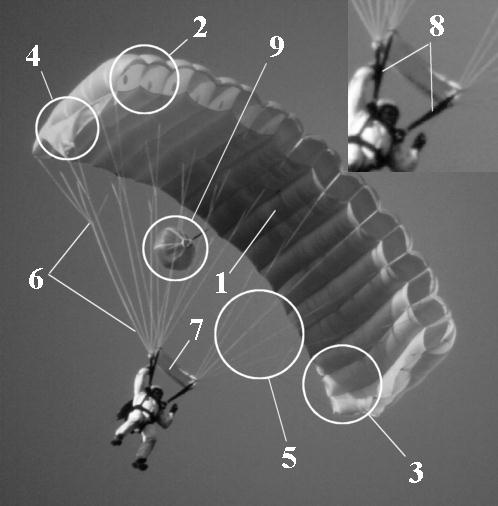
\includegraphics[width=0.7\textwidth]{Paavarjon-osat.jpg}\caption{Päävarjon osat: 1. Kupu 2. Tunnelipari 3. Kuvun takahelma 4. Stabilisaattori 5. Kantopunokset 6. Ohjauspunokset 7. Slider 8. Kantohihnat 9. Apuvarjo}\end{figure*} 


Laskuvarjokokonaisuuteen kuuluu reppu-valjasyhdistelmä sekä kaksi varjoa: pää- ja varavarjo. Molemmat näistä ovat liitovarjoja, jotka ovat muodoltaan siiven kaltaisia. Niiden liitosuhde on noin 3:1, eli liitäessään kolme metriä eteenpäin varjo vajoaa metrin.  


\begin{Figure}\centering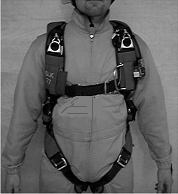
\includegraphics[width=0.7\textwidth]{Reppu-valjas-etu.png}\captionof{figure}{Wings-reppuvaljasyhdistelmä hyppääjän päällä}\end{Figure} 

\subsection{ Päävarjo }
\label{laskuvarjokalusto-ja-hyppyvarusteet-paavarjo}


Päävarjo, joka koostuu kuvusta, punoksista ja sliderista, on kantohihnojen välityksellä kiinni valjaissa kolmirengaslukkojen avulla. Kupu on rakennettu tunneleista, joiden toinen pää on umpinainen. Eripituisilla kantopunoksilla kuvun kohtauskulma pidetään sellaisena, että etureuna on takareunaa hieman alempana. Liitovarjo muodostaa nostovoimaa samalla tavalla kuin lentokoneen siipi. 

\subsection{ Varavarjo }
\label{laskuvarjokalusto-ja-hyppyvarusteet-varavarjo}


Varavarjo on rakenteeltaan ja toiminnaltaan samanlainen kuin päävarjo. Varavarjoa käytettäessä laskeutumispaikka saattaa olla muualla kuin laskeutumisalueella. Tämän vuoksi alastuloasennon on oltava hyvä ja tarvittaessa on tehtävä maahantulokierähdys. 

\section{ Reppu-valjasyhdistelmä }
\label{laskuvarjokalusto-ja-hyppyvarusteet-reppu-valjasyhdistelma}


\begin{Figure}\centering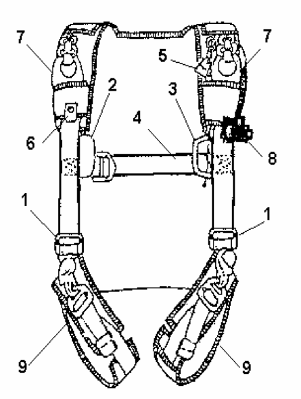
\includegraphics[width=0.6\textwidth]{Reppuvaljasyhdistelma.png}\captionof{figure}{1. Valjaan pystyhihnojen säätösoljet 2. Päävarjon irtipäästöpampula 3. Varavarjon avauskahva 4. Rintahihna 5. Varavarjon pakkolaukaisuhihna RSL 6. Koukkupuukko (sijainti voi vaihdella) 7. Kolmirengasolkalukot 8. FXC-automaattilaukaisimen säätöyksikkö (mikäli käytössä joku muu, merkitse säätöyksikön paikka kuvaan) 9. Reisihihnat}\end{Figure} 


\begin{Figure}\centering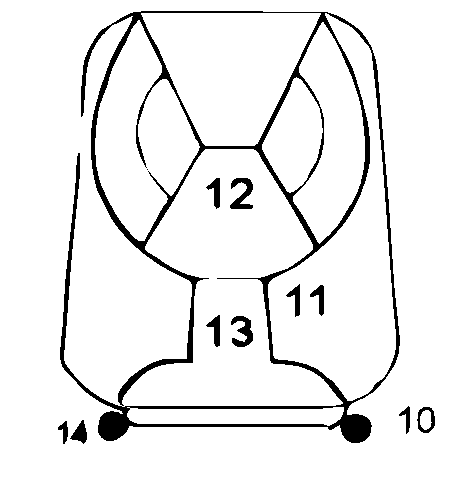
\includegraphics[width=0.6\textwidth]{Reppu-nova.pdf}\captionof{figure}{10. Päävarjon apuvarjo 11. Päävarjon reppu 12. Varavarjon reppu 13. Päävarjon läppä 14. Päävarjon avauskahva hyppymestarille (NOVA-kahva)}\end{Figure} 


\begin{Figure}\centering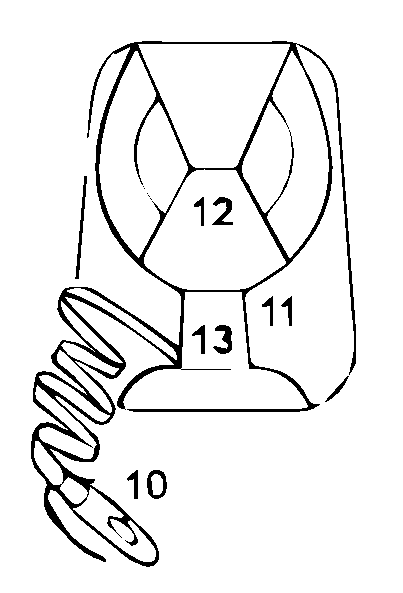
\includegraphics[width=0.6\textwidth]{Reppu-pl.pdf}\captionof{figure}{10. PL-hihna 11. Päävarjon reppu 12. Varavarjon reppu 13. Päävarjon läppä}\end{Figure} 

\section{ Lisälaitteet }
\label{laskuvarjokalusto-ja-hyppyvarusteet-lisalaitteet}


Pää- ja varavarjon lisäksi valjaissa on laitteita lisäämässä hyppääjän turvallisuutta. Näiden laitteiden tarkoituksena on varmistaa varavarjon aukeaminen. 


Varavarjon pakkolaukaisuhihnan (Reserve Static Line, RSL) tarkoituksena on varmistaa varavarjon avautuminen päävarjon irrottua valjaista. Järjestelmä liittää päävarjon kantohihnan ja varavarjon aukaisujärjestelmän yhteen. Hyppääjän on mahdollista vapauttaa varavarjon pakkolaukaisuhihna avaamalla päävarjon kantohihnaan kytketty pikalukko. 


Kun päävarjon kantohihnat ovat päävarjon irtipäästön (\ref{paavarjon-vajaatoiminnot-varavarjon-kaytto} s.\pageref{paavarjon-vajaatoiminnot-varavarjon-kaytto}) jälkeen irronneet kolmirengaslukoista, päävarjo vetää irrotessaan varavarjon pakkolaukaisuhihnasta ja avaa varavarjon. Varavarjon pakkolaukaisuhihna on kuitenkin vain apuväline. Hyppääjän on aina avattava varavarjo vetämällä varavarjon kahvasta! 


\begin{Figure}\centering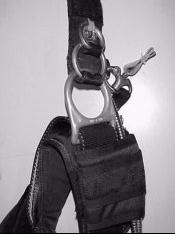
\includegraphics[width=0.7\textwidth]{Kolmirengaslukko.jpg}\captionof{figure}{Kolmirengaslukko}\end{Figure} \begin{Figure}\centering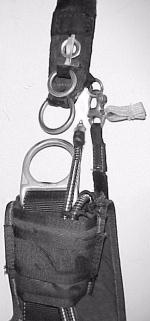
\includegraphics[width=0.7\textwidth]{Kolmirengaslukko-auki.jpeg}\captionof{figure}{Kolmirengaslukko on auennut. Päävarjon kantohihna vetää irrotessaan RSL-hihnasta.}\end{Figure} 


Toinen lisälaite varavarjon aukaisuun on automaattilaukaisin (Automatic Activation Device, AAD). Käytössä on kahta eri tyyppiä: mekaaninen (FXC) ja elektroninen (Cypres ja Vigil). Laitteiden tarkoitus on avata varavarjo, jos hyppääjä putoaa liian kovalla vauhdilla liian matalalla. Molemmat laitteet on säädetty toimimaan määrätyssä korkeudessa (n. 300 m).  


Oppilaan ollessa kyseessä vain hyppymestarilla on oikeus säätää automaattilaukaisinta. FXC:n säätölaitteessa on JUMP/OFF-nuppi, jonka on koko ajan oltava JUMP-asennossa. On olemassa kaksi tilannetta, joissa FXC:n JUMP/OFF-nuppi käännetään OFF-asentoon: 

\begin{itemize}
\item  Koneella alas tultaessa hyppymestarin käskystä 
\item  Laskeuduttaessa veteen (\ref{mahdolliset-vaaratilanteet-laskeutuminen-veteen} s.\pageref{mahdolliset-vaaratilanteet-laskeutuminen-veteen}) 
\end{itemize}

\begin{Figure}\centering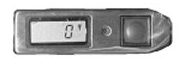
\includegraphics[width=0.7\textwidth]{AAD-Cypres.jpg}\captionof{figure}{Cypres-automaattilaukaisimen käyttöyksikkö}\end{Figure} 

\section{ Muut hyppytoiminnassa käytettävät varusteet }
\label{laskuvarjokalusto-ja-hyppyvarusteet-muut-hyppytoiminnassa-kaytettavat-varusteet}

\begin{itemize}
\item  Kova kypärä, jossa kiinnityshihna on kypärän ulkopuolella. 
\item  Radiovastaanotin on oltava ainakin kolmella ensimmäisellä hypyllä. 
\item  Suojalasit suojaavat silmiä viimalta ja roskilta. 
\item  Haalari, jossa ei saa olla tarttuvia taskuja tai ulokkeita, jotka voivat takertua johonkin tai joista hyppääjä voi vahingossa ottaa kiinni kahvoista kiinni ottaessaan. Haalarin alle puetaan säähän sopiva vaatetus, joka ei haittaa liikkumista. 
\item  Sormikkaat ovat pakolliset oppilailla. Niiden on oltava lämpimät, mutta ei liian paksut eikä liukkaat. 
\item  Kengät, joiden on oltava hyppytoimintaan soveltuvat (ei koukkuja tms.). 
\item  Korkeusmittari, joka nollataan maassa. Mittari kiinnitetään rintahihnaan tai käteen. 
\item  Koukkupuukkoa käytetään takertumien selvittämiseen sotkeutumis- tai törmäämistilanteissa. 
\item  Pelastusliivi puetaan koulutuspäällikön harkinnan mukaan, jos hyppypaikalla on ilmeinen hukkumisvaara. 
\end{itemize}

Hypyn aikana mukana ei saa olla mitään tarpeetonta (esimerkiksi avaimet, kynä tai matkapuhelin). Lisäksi aina hyppäämään tultaessa on oltava mukana hyppypäiväkirja. 

\section{ Hyppyvarusteiden käsittely }
\label{laskuvarjokalusto-ja-hyppyvarusteet-hyppyvarusteiden-kasittely}


Suojaa varjoa auringonvalolta, kosteudelta ja likaantumiselta. Nosta valjaita olkahihnoista ja varo tarttumasta aukaisukahvoihin sekä vaijereiden suojaputkiin. Varjoa ei tule heitellä, laahata eikä sen päällä tule istua. Älä tupakoi, kun olet pukenut valjaat päälle. 


Oppilaan päävarjon pakkaamista saa valvoa henkilö, jolla on itsenäisen hyppääjän kelpoisuus. Oppilaan käytössä olevan päävarjon pakkauksista ja pakkaustarkistuksista pidetään kirjaa. Varavarjon saa pakata vain siihen koulutuksen saanut henkilö. Varusteet palautetaan aina hypyn jälkeen omille paikoilleen. 

\section{ 3X3 -tarkastus }
\label{laskuvarjokalusto-ja-hyppyvarusteet-3x3-tarkastus}


Peruskoulutusvaiheessa oppilaalle opetetaan varusteiden perusteellinen tarkastus, mutta itseaukaisuvaiheessa varjon perustarkastus voidaan tiivistää 3X3 -tarkastukseen (kolme kolmea -tarkastus): 

\begin{enumerate}[label=\bfseries \arabic*)]
\item  Tarkastetaan, että solkia on kiinni kolme: 
	\begin{itemize}
	\item  Vasemman jalkahihnan solki 
	\item  Oikean jalkahihnan solki 
	\item  Rintahihnan solki 
	\end{itemize}
\item  Tarkastetaan, että kahvoja on kolme ja ne ovat kiinni: 
	\begin{itemize}
	\item  Päävarjon avauskahva 
	\item  Päävarjon irtipäästöpampula 
	\item  Varavarjon avauskahva 
	\end{itemize}
\item  Tarkastetaan, että kolmirengaslukot ovat kiinni ja oikein. 
\end{enumerate}
\end{multicols}

\chapter{Hyppytapahtuma}
\label{hyppytapahtuma}
\thispagestyle{headings}
\begin{multicols}{2}
\section{ Valmistautuminen hyppyyn }
\label{hyppytapahtuma-valmistautuminen-hyppyyn}


Hyppytapahtuma ei suinkaan ala siitä, kun poistutaan koneesta ilmassa. Jotta kaikki sujuisi hyvin, on tärkeää huolehtia myös valmisteluista. Päätös hypätä on hyvä tehdä jo edellisenä päivänä, sillä näin ehtii henkisesti valmistautua tulevaan suoritukseen. Riittävä yöuni ja ravinto ovat myös tärkeitä – väsyneenä tai nälkäisenä keskittyminen on vaikeaa. 


Ennen hyppäämään kirjoittautumista (pokalistan täyttöä) kootaan kaikki tarvittavat varusteet ja ilmoittaudutaan hyppäämään. Varusteita on hyvä sovittaa päälle, jotta niihin voi tehdä tarvittavat säädöt ajoissa ennen koneelle lähtöä. Suoritusta harjoitellaan joko itsenäisesti tai hyppymestarin kanssa. 


Mikäli mahdollista, seuraa ennen omaa pokaasi toisten hyppääjien ohjailua varjon varassa nähdäksesi ylä- ja pintatuulien vaikutuksen ohjaamiseen ja laskeutumiseen. 


Ennen koneelle menoa hyppymestari tarkastaa, että varusteet on puettu oikein päälle. Tarkastuksen jälkeen varusteita \textbf{ei saa säätää} ilman hyppymestarin lupaa! Vallitsevan tuulen mukainen ohjauskuvio (\ref{hyppytapahtuma-laskeutumiskuvio} s.\pageref{hyppytapahtuma-laskeutumiskuvio}) käydään vielä läpi ennen koneelle menoa. Oppilaat saavat mennä koneelle vain hyppymestarin johdolla. 

\subsection{ Toiminta koneessa }
\label{hyppytapahtuma-toiminta-koneessa}


Kone kuormataan yleensä käänteisessä järjestyksessä eli se, joka menee koneeseen ensimmäisenä, hyppää viimeisenä (poikkeuksena hyppymestari). Varo varusteiden tarttumista koneessa oleviin ulokkeisiin aina koneessa liikkuessasi. Suojaa erityisesti varjojen aukaisukahvoja myös muiden liikkuessa. Jos takerrut kiinni johonkin, älä revi itseäsi irti väkisin, vaan ilmoita asiasta hyppymestarille. Vältä turhaa liikkumista. Pidä mahdolliset istuinvyöt kiinni, kunnes hyppymestari aukaisee ne tai antaa luvan aukaisuun. Ilmailumääräyksen OPS M6-1 perusteella ilma-aluksella saa kuljettaa sen päällikön ja hyppääjien suostumuksella ja omalla vastuulla enintään kymmentä hyppääjää ilman istuinvyötä.  


Jos lennon aikana huomaat omissa tai muiden varusteissa jotain poikkeavaa, ilmoita siitä heti hyppymestarille. Keskity omaan hyppyysi. Huomioi muut koneessa olijat äläkä häiritse heidän keskittymistään. Koneen päällikkö on lentäjä, mutta sinun päällikkösi on hyppymestari. Lähestyttäessä uloshyppypaikkaa kone lentää tuuliolosuhteiden perusteella määriteltyä linjaa. Hyvissä ajoin ennen uloshyppypaikkaa hyppymestari tarkastaa vielä oppilaiden varusteet. 

\section{ Uloshyppy Cessna 206, pakkolaukaisu }
\label{hyppytapahtuma-uloshyppy-cessna-206-pakkolaukaisu}


Hyppymestarin komennolla OVELLE! siirrytään (varoen repun osumista koneeseen) ovelle uloshyppyasentoon. Komennolla MENE! ponnistetaan irti koneesta, otetaan hyvä taivutus ja delta-asento sekä aletaan laskea. Rintamasuunnan on pysyttävä koko ajan suoraan koneen lentosuuntaan. 


\begin{Figure}\centering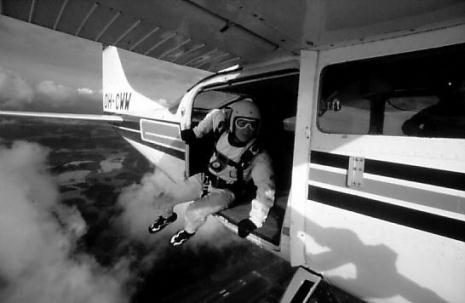
\includegraphics[width=0.7\textwidth]{206UH1.jpeg}\captionof{figure}{Hyppääjä on siirtymässä ovelle uloshyppyasentoon}\end{Figure} 


Uloshypyssä maa vetää helposti katsetta puoleensa. Jos katsoo maahan eikä koneeseen, taivutus todennäköisesti kääntyy väärin päin. Ihmisen vartalo kääntyy yleensä katseen suuntaan, joten kun uloshypyn aikana katsoo ylös koneeseen, niin vartalo on taipunut oikeanlaiselle kaarelle. Taivutus lähtee lantiosta (myös selkä ja niska). 


Tärkeintä uloshypyssä on taivutus. Delta-asennossa kädet ovat n. 45 astetta irti kyljistä, olkapäät takana. Jalat pidetään noin hartioiden levyisessä haara-asennossa ja vain hiukan koukistettuna. 


Laskeminen on tärkeää opetella heti alusta alkaen, sillä se on käytännössä ainoa tapa säilyttää ajantaju tässä vaiheessa hyppyuraa. Laskeminen tapahtuu ääneen huutamalla (101...105). Uloshyppyharjoituksissa opetellaan oikeaa rytmiä, joten ei huudeta vain numeroita vaan sekunteja. Ilmassa muutama sekunti voi tuntua hyvinkin pitkältä ajalta. 


\begin{Figure}\centering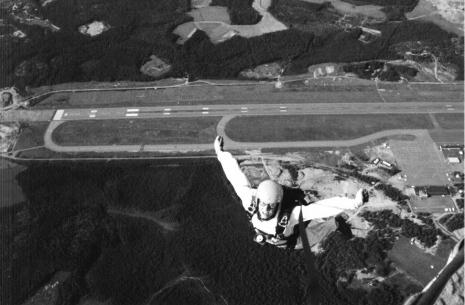
\includegraphics[width=0.7\textwidth]{206UH2.jpeg}\captionof{figure}{Hyppääjä on ponnistanut irti koneesta.}\end{Figure} 


Onnistuneen uloshypyn päätekijät ovat: 

\begin{itemize}
\item  Asettautuminen hyvään uloshyppyasentoon ovelle (katse ylös koneeseen) 
\item  Riittävä ponnistus ja rintamasuunta lentosuuntaan  
\item  Hyvä ja symmetrinen delta-asento sekä voimakas taivutus ja katse ylös koneeseen 
\end{itemize}
\section{ Uloshyppy Streevakone, pakkolaukaisu }
\label{hyppytapahtuma-uloshyppy-streevakone-pakkolaukaisu}


Hyppymestarin komennolla OVELLE! siirrytään ovelle. Komennolla MENE! siirrytään (varoen repun osumista koneeseen) roikkumaan streevalle uloshyppyasentoon, irrottaudutaan koneesta ja pidetään hyvä taivutus sekä X-asento ja aletaan laskea. Rintamasuunnan on pysyttävä koko ajan suoraan koneen lentosuuntaan. 


\begin{Figure}\centering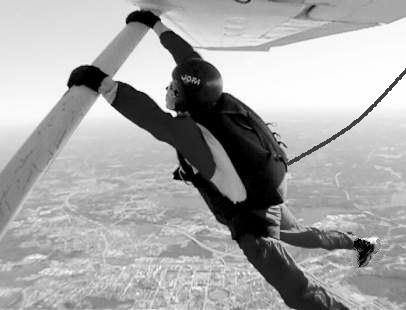
\includegraphics[width=0.7\textwidth]{Streeva-UH1.jpeg}\captionof{figure}{Hyppääjä on siirtynyt streevalle uloshyppyasentoon}\end{Figure} 


Uloshypyssä maa vetää helposti katsetta puoleensa. Jos katsoo maahan eikä koneeseen, taivutus kääntyy todennäköisesti väärin päin. Ihmisen vartalo kääntyy yleensä katseen suuntaan, joten kun katsoo uloshypyn aikana ylös kohti konetta, vartalo on taipunut oikeanlaiselle kaarelle. Taivutus lähtee lantiosta (myös selkä ja niska). 


Mikäli taivutuksesi syystä tai toisesta häviää, voit korjata tilanteen helposti: taivuttamalla. 


Tärkeintä uloshyppyasennossa ja uloshypyssä on siis taivutus. X-asennossa kädet ovat ylhäällä levitettyinä, olkapäät takana. Jalat pidetään noin hartioiden levyisessä haara-asennossa ja vain hiukan koukistettuna. 


Laskeminen on tärkeää opetella heti alusta alkaen, sillä se on käytännössä ainoa tapa säilyttää ajantaju tässä vaiheessa hyppyuraa. Laskeminen tapahtuu ääneen huutamalla (101...105). Uloshyppyharjoituksissa opetellaan oikeaa rytmiä, joten ei huudeta vain numeroita vaan sekunteja. Ilmassa muutama sekunti voi tuntua hyvinkin pitkältä ajalta. 


\begin{Figure}\centering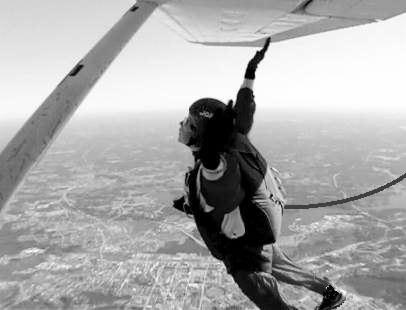
\includegraphics[width=0.7\textwidth]{StreevaUH2.jpeg}\captionof{figure}{Hyppääjä on irroittautunut koneesta.}\end{Figure} 


Onnistuneen uloshypyn päätekijät ovat: 

\begin{itemize}
\item  Asettautuminen hyvään ja symmetriseen uloshyppyasentoon (X-asento, taivutus ja katse ylös koneeseen) 
\item  Käsien yhtäaikainen irrottaminen ja rintamasuunta lentosuuntaan  
\item  Hyvä ja symmetrinen X-asento sekä voimakas taivutus ja katse ylös koneeseen 
\end{itemize}
\section{ Uloshyppy NOVA }
\label{hyppytapahtuma-uloshyppy-nova}


Hyppymestari komentaa: \textbf{SIIRRY / YLÖS} 


Siirry- tai Ylös-komennolla valmistaudut siirtymään ovelle.  


Hyppymestari komentaa: \textbf{OVELLE} 


Ovelle-komennolla hyppymestari auttaa sinua, kun siirryt ovelle (varoen repun osumista koneeseen) uloshyppyasentoon, jolloin kummatkin hyppymestarit pitävät sinusta kiinni. Tarvittaessa sisällä oleva hyppymestari antaa lisäkomentoja. 


Kun olet valmis, siirrä katseesi sisäpuolella olevaan hyppymestariin ja tee uloshyppytarkistus. Eli pidä katseesi hyppymestarissa ja sano kovalla äänellä: 


\textbf{TARKISTUS SISÄÄN} 


Tällä varmistat sisällä olevan hyppymestarin valmiuden, joka ollessaan valmis nyökkää jolloin voit jatkaa eteenpäin. Pidä katseesi hyppymestarissa niin kauan kunnes hän antaa merkin ravistamalla tai nyökkäämällä. 


Tämä jälkeen tarkista ulkona olevan hyppymestarin valmius. Siirrä katseesi olkapääsi yli ulos hyppymestariin ja sano kovalla äänellä: 


\textbf{TARKISTUS ULOS} 


Tällä varmistat ulkona olevan hyppymestarin valmiuden, joka ollessaan valmis nyökkää jolloin voit jatkaa eteenpäin. Pidä katseesi hyppymestarissa niin kauan, kunnes hän antaa merkin ravistamalla tai nyökkäämällä. 


Kun olet varmistanut hyppymestareiden valmiuden voit aloittaa rytmikkään uloshyppylaskennan ääneen. Laskenta voi vaihdella käytetyn konetyypin mukaan. 

\begin{description}
\item[\textbf{SIIPI}] \hfill \\ 
Siirrä ja pidä katseesi siivessä (tai vastaavassa kiintopisteessä) \hfill \\ 
\item[\textbf{YLÖS} (tai ULOS)] \hfill \\ 
Liikuta vartaloasi ylöspäin (tai ulospäin) \hfill \\ 
\item[\textbf{ALAS} (tai SISÄÄN)] \hfill \\ 
Liikuta vartaloasi alaspäin (tai sisäänpäin) \hfill \\ 
\item[\textbf{TAIVUTA}] \hfill \\ 
Ponnista sivuttain ulospäin, ota hyvä taivutus ja siirrä välittömästi kädet ja jalat symmetrisesti vapaapudotusasentoon. Pidä katseesi koneessa mahdollisimman pitkään koko uloshypyn ajan, sillä se edesauttaa hyvää uloshyppyä. Laske myös ääneen 105 saakka ja aloita hypyn kulku. \hfill \\ 
\end{description}

Laskeminen on tärkeää opetella heti alusta, sillä se on käytännössä ainoa tapa säilyttää ajantaju tässä vaiheessa hyppyuraa. Laskeminen tapahtuu ääneen huutamalla (101...105). Uloshyppyharjoituksissa opetellaan oikeaa rytmiä, joten ei huudeta vain numeroita vaan sekunteja. Ilmassa muutama sekunti voi tuntua hyvinkin pitkältä ajalta. 

\section{ Vapaapudotuksen perusteet }
\label{hyppytapahtuma-vapaapudotuksen-perusteet}

\begin{description}
\item[ ] \hfill \\ 
\textit{Jos olet pakkolaukaisukurssilla, voit siirtyä kohtaan: Varjon avautuminen ja lentokuntoon saattaminen, (\ref{hyppytapahtuma-varjon-avautuminen-ja-lentokuntoon-saattaminen} s.\pageref{hyppytapahtuma-varjon-avautuminen-ja-lentokuntoon-saattaminen}) ja palata tähän lukuun kun olet siirtymässä itseaukaisuhyppyihin.} \hfill \\ 
\end{description}

\begin{figure*}[]\centering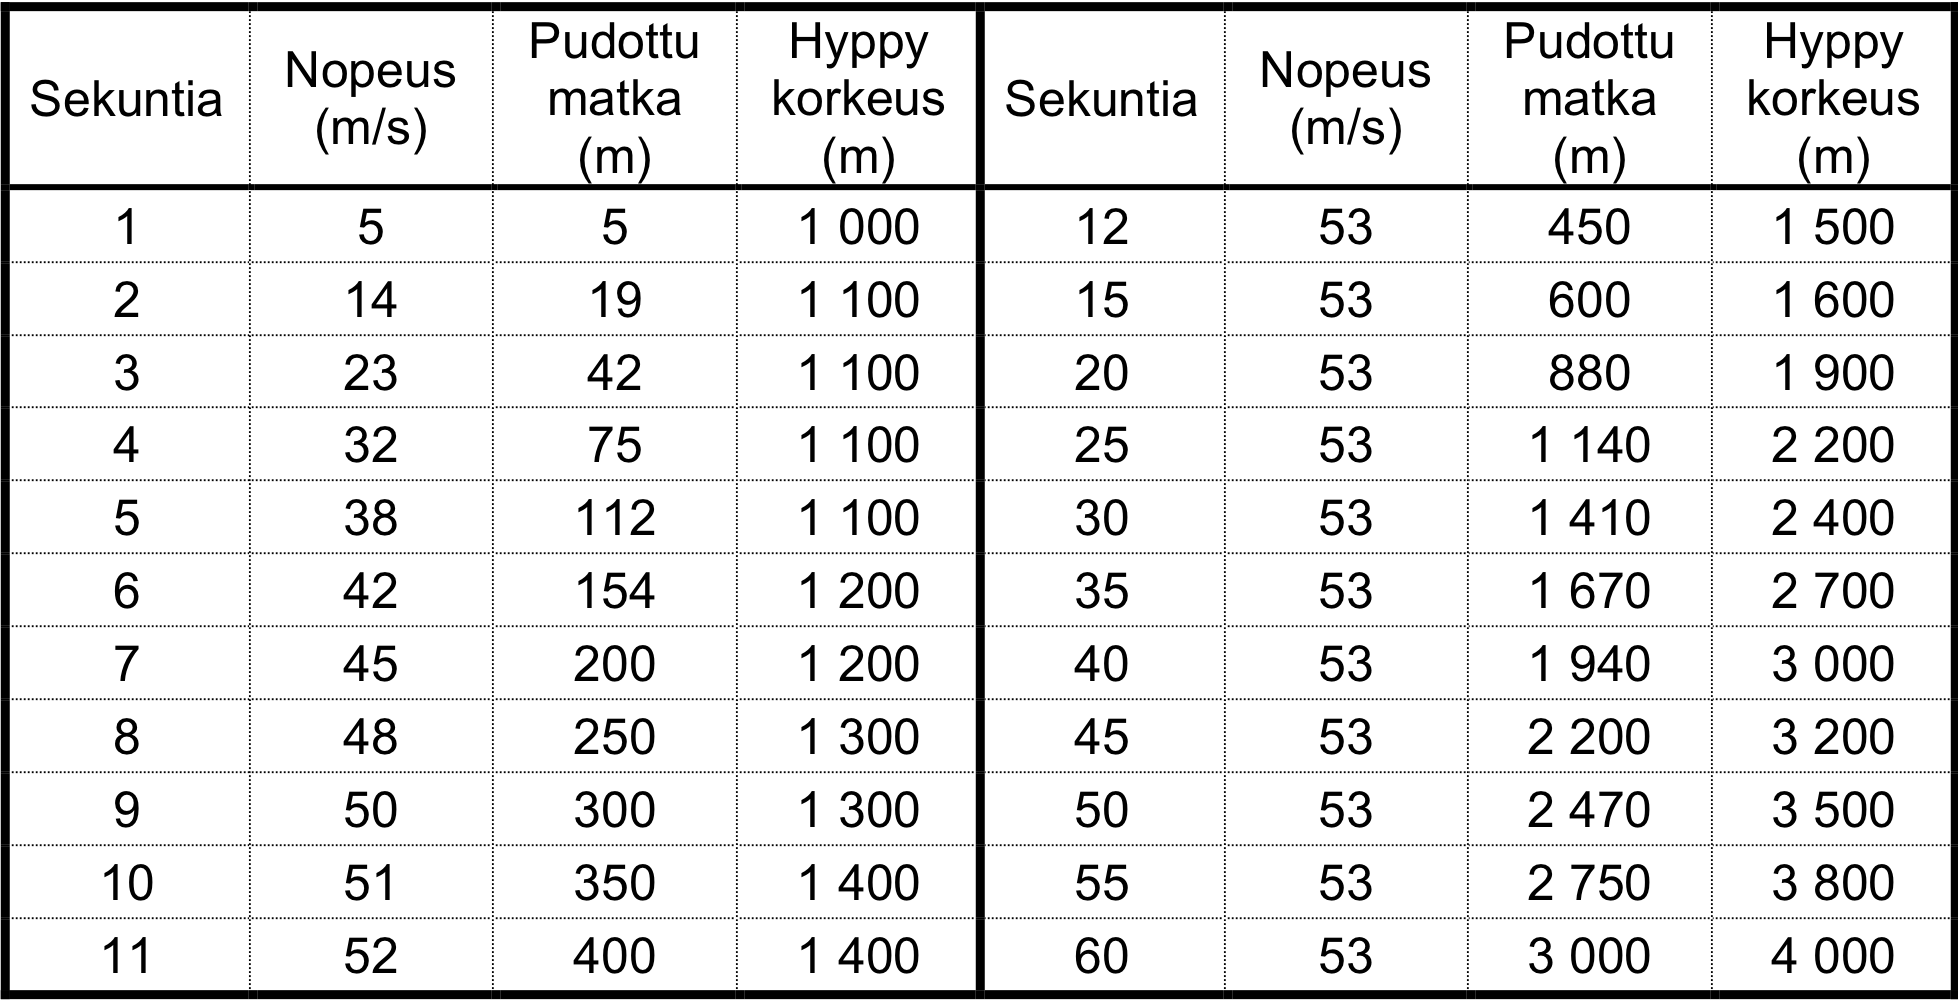
\includegraphics[width=0.7\textwidth]{Vapaapudotus-taulukko.png}\caption{Hyppääjän keskimääräinen nopeus ja pudottu matka ajan suhteen.}\end{figure*} 


Maan vetovoimasta johtuen nopeus vapaapudotuksessa kiihtyy. Ilmanvastuksen vaikutuksesta putoamisnopeudeksi vakiintuu 10–12 sekunnin kuluttua 180–190 km/h (50-53 m/s). 


Seuraavaan taulukkoon on koottuna hyppääjän keskimääräinen nopeus (maata kohti), pudottu matka hypyn alusta lähtien sekä laskennallinen hyppykorkeus, jos varjo avataan 1000 metrin korkeudessa. Putoamisnopeus riippuu mm. hyppääjän massasta, asennosta, vaatetuksesta ja hyppykorkeudesta. 


Kaikilla oppilaskoulutushypyillä varjo on avattava aina viimeistään 1000 metrin korkeudessa. Jos avaus jostain syystä tapahtuu alle 800 metrin korkeudessa, on asiasta ilmoitettava heti kouluttajalle. Jos käytössä on FXC-12000-automaattilaukaisin, on se todennäköisesti herkistynyt ja saattaa seuraavalla hypyllä avata varavarjon virheellisesti. 

\subsection{ Korkeusmittarin käyttö vapaassa }
\label{hyppytapahtuma-korkeusmittarin-kaytto-vapaassa}


\begin{figure*}[]\centering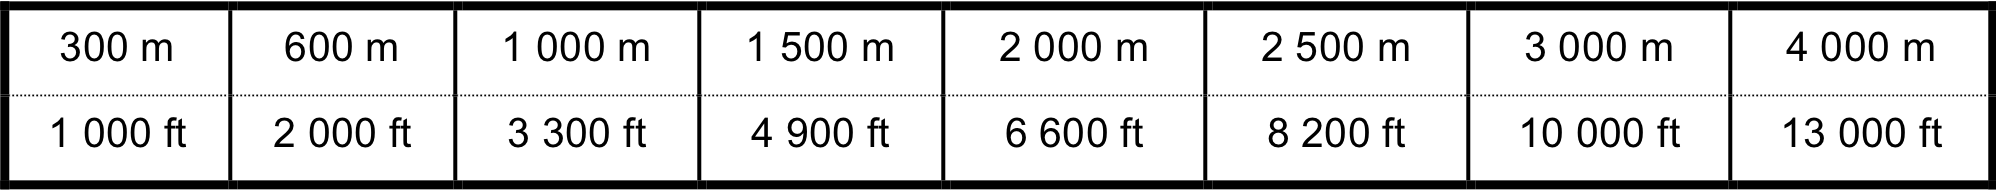
\includegraphics[width=0.8\textwidth]{Metrit-jaloiksi-taulukko.png}\caption{Nämä pyöristetyt muunnokset tulee osata hyppytoiminnassa.}\end{figure*} 


Kaikilla laskuvarjohypyillä on käytettävä visuaalista korkeusmittaria. Poikkeuksena ovat vesihypyt, joilla hyppykorkeus ei ylitä 1500 metriä. Mittarit perustuvat ilmanpaineen muutokseen. Ilmanpaine pienenee noin 1 mbar / 8 m ylöspäin mentäessä.  


Pakkolaukaisukurssin käyneet oppilaat alkavat harjoitella mittarin käyttöä 5 sekunnin vapaapudotushypystä lähtien. Ensin mittarin käyttöön totutellaan laskemisen määrätessä varjon avaushetken. Jo 10 sekunnin vapaapudotushypyllä on laskeminen vain varmistuskeino toimivan mittarin määritellessä avauskorkeuden. Seuraa korkeutta jatkuvasti noin viiden sekunnin välein. 


Korkeusmittarit jaetaan kahteen pääryhmään, visuaalisiin ja äänikorkeusmittareihin. Visuaalisesta mittarista luetaan hyppykorkeus, purku- ja avauskorkeus, päätöskorkeus varavarjotilanteessa sekä ohjaamiseen liittyvät korkeudet. Äänikorkeusmittarit hälyttävät ennalta asetetussa korkeudessa tai korkeuksissa.  


Visuaalinen, metriasteikolla varustettu osoitinmittari, on ainoa hyväksyttävä mittari hyppyuran alussa.   


Visuaalisessa korkeusmittarissa on 

\begin{itemize}
\item  näyttöväli 10, 50 tai 100 metriä ja numerot 100 tai 500 metrin välein. 
\item  avauskorkeus 800 tai 1000 metriä merkitty eri värillä. 
\item  joko osoitinmittari tai digitaalinen, jossa numeronäyttö. 
\end{itemize}

Mittarin näyttöasteikko voi osoittaa korkeuden joko metreinä tai jalkoina (feet = ft). Jalka = 0,3048 m. 

\subsection{ Käyttö }
\label{hyppytapahtuma-kaytto}


Korkeusmittaria käytettäessä on huomioitava seuraavat asiat: 

\begin{itemize}
\item  Mittari on asetettava paikkaan, josta se nähdään aina. 
\item  Perusasennon on säilyttävä mittaria katsottaessa. 
\item  Mittaria vilkaistaan päätä kääntämällä tai FS-hypyillä voidaan katsoa myös muiden mittareita. 
\item  Mittaria luetaan vertaamalla viisarin asentoa punaisen alkuun eikä numeroihin tuijottamalla. 
\item  Ajantajun on säilyttävä jokaisella hypyllä, sillä mittari voi mennä rikki.  
\item  Mittarin jumiutuessa, tai jos mittari ei ole luettavissa, avataan varjo heti, mutta huomioidaan kuitenkin muut hyppääjät. 
\item  Freehypyillä suositellaan käsimittaria. Ensimmäisillä freehypyillä kannattaa käyttää myös rintamittaria. 
\item  Käytettäessä integraalikypärää suositellaan käsimittaria, sillä rintamittari ei ole välttämättä luettavissa. 
\item  Mittarit on kalibroitu toimimaan tarkimmin avauskorkeusalueella. Korkealla esiintyvät näyttöerot ovat tavallisia.  
\end{itemize}
\subsection{ Virheet }
\label{hyppytapahtuma-virheet}


Yleisimmät viat ja virheet korkeusmittarin toiminnassa ovat: 

\begin{itemize}
\item  paine-erot ja virhenäytöt vapaapudotushypyillä esimerkiksi käytettäessä rintamittaria selkälennossa 
\item  mittarin jäätyminen kosteuden tai tiivistyneen veden takia 
\item  jumiutuminen iskujen tai lian takia 
\item  mekaaninen vika, joka aiheutuu mittarin pudotessa maahan tai maassa olevan mittarin päälle astumisesta 
\item  paristojen loppuminen 
\end{itemize}

Korkeuserojen laskeminen ja mittariasetus on osattava, jos lähtö- ja alastulopaikka eivät ole samat. 


\end{multicols}\pagebreak\begin{multicols}{2} 

\section{ Avaaminen }
\label{hyppytapahtuma-avaaminen}

\subsection{ Avauksen tärkeysjärjestys }
\label{hyppytapahtuma-avauksen-tarkeysjarjestys}

\begin{framed}
\begin{enumerate}[label=\bfseries \arabic*)]
\item  \textbf{Avaa varjo.} Itseaukaisuhypyllä tärkein tehtäväsi on aina avata itse varjosi. 
\item  \textbf{Avaa avauskorkeudessa} Jokaiselle hypyllä on aina määrätty avauskorkeus, jossa varjo on ehdottomasti avattava. 
\item  \textbf{Avaa stabiilissa asennossa} Pyri avaamaan varjosi stabiilissa asennossa, mutta tärkeämpää on avata oikeassa korkeudessa. 
\end{enumerate}
\end{framed}

\subsection{ Avausjärjestelmät }
\label{hyppytapahtuma-avausjarjestelmat}

\subsubsection{ Jousiapuvarjo  }
\label{hyppytapahtuma-jousiapuvarjo}


Jousikuormitettu apuvarjo kiinnitetään yhdyspunoksella sisäpussin kautta päävarjoon. Jousi on malliltaan joko kartion muotoinen tai tasapaksu. Jousiapuvarjo on kokonaan F-111-kangasta tai valmistettu osittain harsokankaasta. Jousiapuvarjo on alaosastaan avonainen tai suljettu. Jousiapuvarjolla avaaminen tapahtuu vetämällä avauskahvasta. Pidä kahva kädessäsi ja laita se talteen avauksen jälkeen. 

\subsubsection{ Kädestä päästettävä apuvarjo (HD) }
\label{hyppytapahtuma-kadesta-paastettava-apuvarjo-hd}


Avattaessa HD-avausjärjestelmällä apuvarjo heitetään reippaasti puhtaaseen ilmavirtaan. Kädestä päästettävän apuvarjon heittäminen käännöksen tai lattakierteen aikana aiheuttaa aina avautumisongelmia, kuten kierrettä. Jos avausasento ei ole stabiili, jää HD-apuvarjo myös helpommin kiinni hyppääjän varusteisiin ja raajoihin.  


Jousiapuvarjolla aloittaneen oppilaan pitää saada koulutus siirtyessään HD-apuvarjoon. Koulutuksen jälkeen on osattava HD-apuvarjon heittäminen vapaaseen ilmatilaan hyppääjän aiheuttamien pyörteiden ulkopuolelle. Vähintään ensimmäisellä HD-hypyllä (HD-totuttelu) ei tehdä muita suorituksia. HD-totuttelun jälkeen ei pitäisi palata enää kahvavetoisiin varusteisiin. 


\begin{Figure}\centering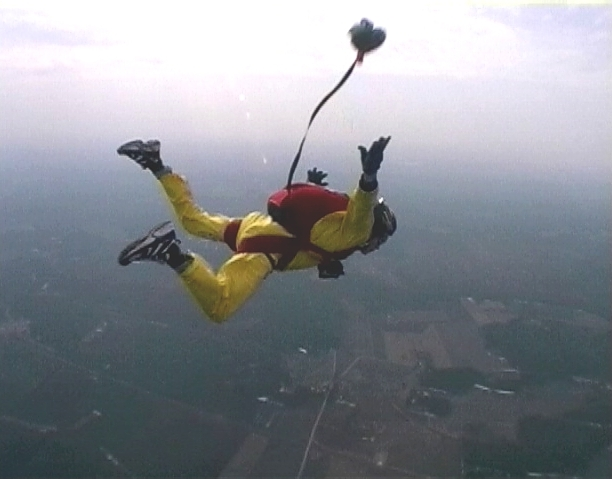
\includegraphics[width=0.8\textwidth]{HD-apuvarjo.jpeg}\captionof{figure}{Hyppääjä on heittänyt HD-apuvarjon ja on palauttamassa käsiään perusasentoon}\end{Figure} 

\subsection{ Vaaratilanteet }
\label{hyppytapahtuma-vaaratilanteet}

\begin{itemize}
\item  Epästabiili asento, kädet/käsi tai jalat/jalka sisällä ⇨ kaatuu kyljelleen/selälleen ⇨ mahdollista sotkeutua avautuvaan varjoon. 
\item  Veto irtipäästöpampulasta ⇨ päävarjo irtoaa normaalin avauksen jälkeen ⇨ tehdään varavarjotoimenpiteet. 
\item  Veto varavarjon kahvasta ⇨ varavarjo aukeaa. 
\item  Veto valjaista / kahva ei lähde / ei vetoa ⇨ päävarjo ei aukea ⇨ uusitaan veto tai tehdään varavarjotoimenpiteet. 
\item  Apuvarjo tarttuu kiinni hyppääjään ⇨ yksi irrotusyritys, jos nähtävissä ⇨ aukeaa tai varavarjotoimenpiteet. 
\item  Punokset sotkeutuvat hyppääjään ⇨ pyritään irrottautumaan sotkeutuneista punoksista, käytetään tarvittaessa koukkupuukkoa ⇨ tehdään varavarjotoimenpiteet. 
\item  Apuvarjo voi avauksessa joskus tulla kuvun etureunan kautta kuvun alapuolelle ⇨ tehdään ohjauskokeilu ⇨ jos varjo ei käyttäydy normaalisti, tehdään varavarjotoimenpiteet.  
\item  Asento hallitsematon ⇨ avataan päävarjo heti. 
\item  Apuvarjo turbulenssissa: 
\end{itemize}

Avauksessa apuvarjo voi jäädä hyppääjän selän taakse muodostuvaan pyörteeseen eli turbulenssiin. Jos vedon jälkeen 105:n kohdalla ei ole tapahtunut mitään, vilkaistaan olkapään yli. Asento kallistuu ja apuvarjon pitäisi saada ilmaa. Ellei varjo avaudu, tehdään varavarjotoimenpiteet, koska apuvarjo tai yhdyspunos on saattanut tarttua johonkin kiinni tai reppu on jumissa. Kiinnitarttumista voidaan yrittää irrottaa, jos varmuudella nähdään ongelman aiheuttaja. Jos irrotus ei onnistu yhdellä yrityksellä tai ongelman aiheuttajaa ei nähdä, tehdään varavarjotoimenpiteet heti. 


\begin{Figure}\centering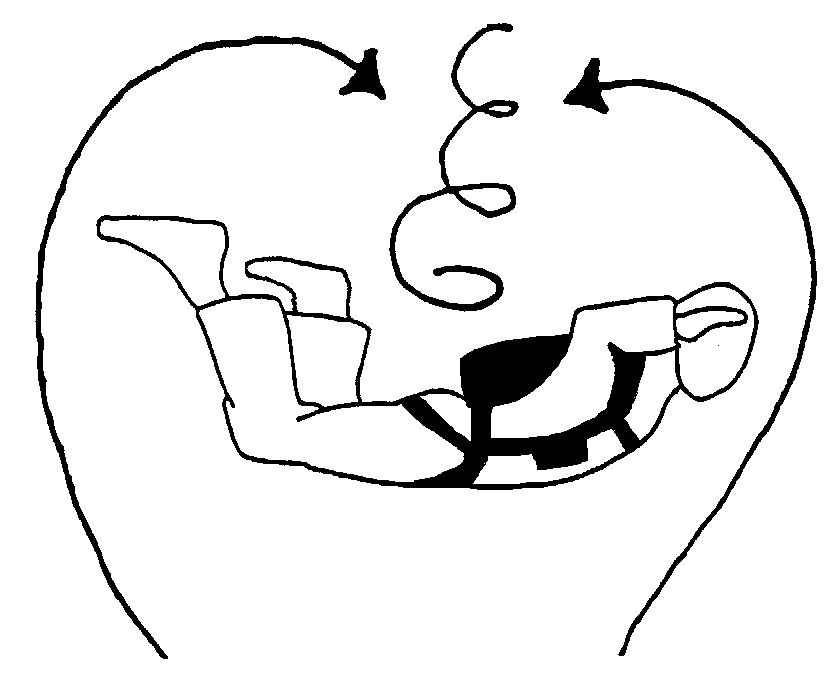
\includegraphics[width=0.7\textwidth]{Selka-turbulenssi.png}\captionof{figure}{Hyppääjän selän taakse muodostuu turbulenssi}\end{Figure} 

\section{ Varjon avautuminen ja lentokuntoon saattaminen }
\label{hyppytapahtuma-varjon-avautuminen-ja-lentokuntoon-saattaminen}


Pakkolaukaisujärjestelmässä koneesta irtautuessa pakkolaukaisujärjestelmä ja vastaavasti NOVA:ssa ilmavirtaan heitetty apuvarjo avaa päävarjon repun jonka jälkeen avausjärjestelmä vetää sisäpussin ulos repusta. Punokset alkavat purkautua kumilenkeistään. Kupu tulee ulos sisäpussista ja alkaa kehittyä keskeltä. Slider liukuu punoksia pitkin alas hidastaen kuvun aukeamista. Sinun tehtäväksesi jää varjon tarkastaminen ja sen lopullinen avaaminen. 


Kun olet päässyt laskemisessa 105:een, tarkasta varjo. Varjo LENTÄÄ, kun 

\begin{itemize}
\item  Kupu on säännöllisen muotoinen 
\item  Punokset ovat kireällä 
\item  Slider on suorakaiteen muotoinen. 
\end{itemize}

Tarkastettuasi varjon vie kädet takimmaisille kantohihnoille. Jos punokset ovat kierteellä, avaa ne potkimalla ja levittämällä kantohihnoja (SELVITÄ). 


Vedä molemmista ohjauslenkeistä (sijaitsevat takimmaisten kantohihnojen takapuolella) alaspäin avataksesi puolijarrut. Puolijarrut saat avata vasta kierteiden poiston jälkeen.  


Tarvittaessa pumppaa slider alas ja tunnelit auki. Pumppaus tehdään vetämällä ohjauslenkit rauhallisesti muutamaksi sekunniksi noin vyötärön tasolle ja palauttamalla ohjauslenkit sitten rauhallisesti takaisin yläasentoon. Pumppauksen voit toistaa useampia kertoja (SELVITÄ).  


Mikäli varjo EI LENNÄ tai EI SELVIÄ, siirry välittömästi varavarjotoimenpiteisiin. (\ref{paavarjon-vajaatoiminnot-varavarjon-kaytto} s.\pageref{paavarjon-vajaatoiminnot-varavarjon-kaytto}) 


Kun olet suorittanut varjon lopullisen avaamisen, tarkasta seuraavat asiat: 

\begin{framed}
\begin{itemize}
\item  ILMATILA (myös kierteiden avauksen ja pumppauksen aikana, väistä tarvittaessa ja/tai varoita huutamalla (\ref{mahdolliset-vaaratilanteet-tormaaminen-varjon-varassa} s.\pageref{mahdolliset-vaaratilanteet-tormaaminen-varjon-varassa})) 
\item  KORKEUS (myös kierteiden avauksen ja pumppauksen aikana) 
\item  KAHVAT taskuissaan (varavarjon kahva ja päävarjon irtipäästöpampula) 
\item  SIJAINTI (oma ja maalialueen sijainti) 
\end{itemize}
\end{framed}

Aloita ohjaaminen ja käännä varjo tarvittaessa vastatuuleen. 


\end{multicols}\pagebreak\begin{multicols}{2} 

\section{ Ohjaaminen }
\label{hyppytapahtuma-ohjaaminen}

\subsection{ Lentotilat }
\label{hyppytapahtuma-lentotilat}

\begin{description}
\item[Täysliito: ] \hfill \\ 
Nosta ohjauslenkit täysin ylös. Varjo saavuttaa suurimman vaakanopeuden ja lentää parhaiten vastatuuleen. \hfill \\ 
\item[Puolijarrutustila: ] \hfill \\ 
Vedä/nosta ohjauslenkit hartioiden korkeudelle. Varjo jarruttaa.  \hfill \\ 
\item[Täysjarrutus: ] \hfill \\ 
Vedä ohjauslenkit noin lantion tasalle. Varjo jarruttaa voimakkaasti. \hfill \\ 
\item[Sakkaus:] \hfill \\ 
Jos ohjauslenkkejä painetaan vielä täysjarrutustilaa alemmaksi, varjo lakkaa lentämästä. Sakkauksessa varjon vajoamisnopeus kasvaa, joten varo sakkaamasta varjoasi matalalla. Varjo palautetaan sakkaustilasta nostamalla ohjauslenkkejä rauhallisesti 10–20 cm. Tämän jälkeen tarkasta varjo ja selvitä sitä tarpeen mukaan. (\ref{paavarjon-vajaatoiminnot} s.\pageref{paavarjon-vajaatoiminnot}) \hfill \\ 
\end{description}

Kokeile varjon eri lentotiloja, mutta muista, että kaikki ohjauskokeilut tulee tehdä yli 600 metrissä. 

%% \end{multicols}{2}
%% \begin{multicols}{2}

\begin{Figure}\centering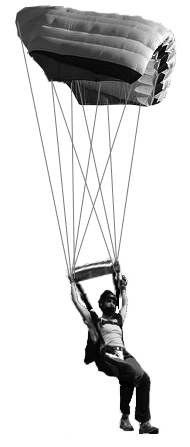
\includegraphics[width=0.5\textwidth]{Lentotila-taysi.jpeg}\captionof{figure}{Täysliito}\end{Figure} \begin{Figure}\centering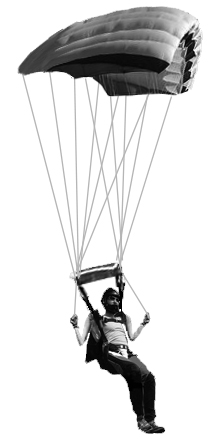
\includegraphics[width=0.5\textwidth]{Lentotila-puoli.jpeg}\captionof{figure}{Puolijarrutus}\end{Figure} 
\begin{Figure}\centering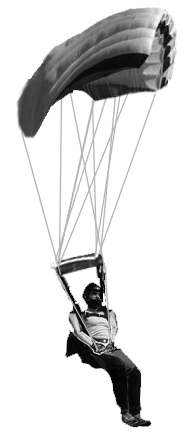
\includegraphics[width=0.5\textwidth]{Lentotila-jarru.jpeg}\captionof{figure}{Täysjarrutus}\end{Figure} 

\subsection{ Ilma- ja maanopeus }
\label{hyppytapahtuma-ilma-ja-maanopeus}


Liitovarjo on hyvin turvallinen, mutta se voi olla suuren suorituskykynsä takia väärin käytettynä hyppääjälle vaarallinen. On tärkeää tietää varjon ominaisuudet ja hallita oikea käyttötapa. 


Liitovarjo lentää ilmassa aina samaa nopeutta täysliidossa (noin 8-10 m/s) tuulista riippumatta. Tätä vakionopeutta kutsutaan ilmanopeudeksi, johon ei vaikuta se, lennetäänkö myötä\mbox{-,} sivu- vai vastatuuleen. Maanopeus on nopeus, jolla varjo liikkuu maahan nähden. Maanopeus muuttuu riippuen siitä, mihin suuntaan tuuleen nähden lennetään. Liitovarjo liikkuu maahan nähden nopeammin myötätuuleen kuin vastatuuleen. Tämän takia liitovarjolla pyritään aina laskeutumaan vastatuuleen. 


\begin{figure*}[]\centering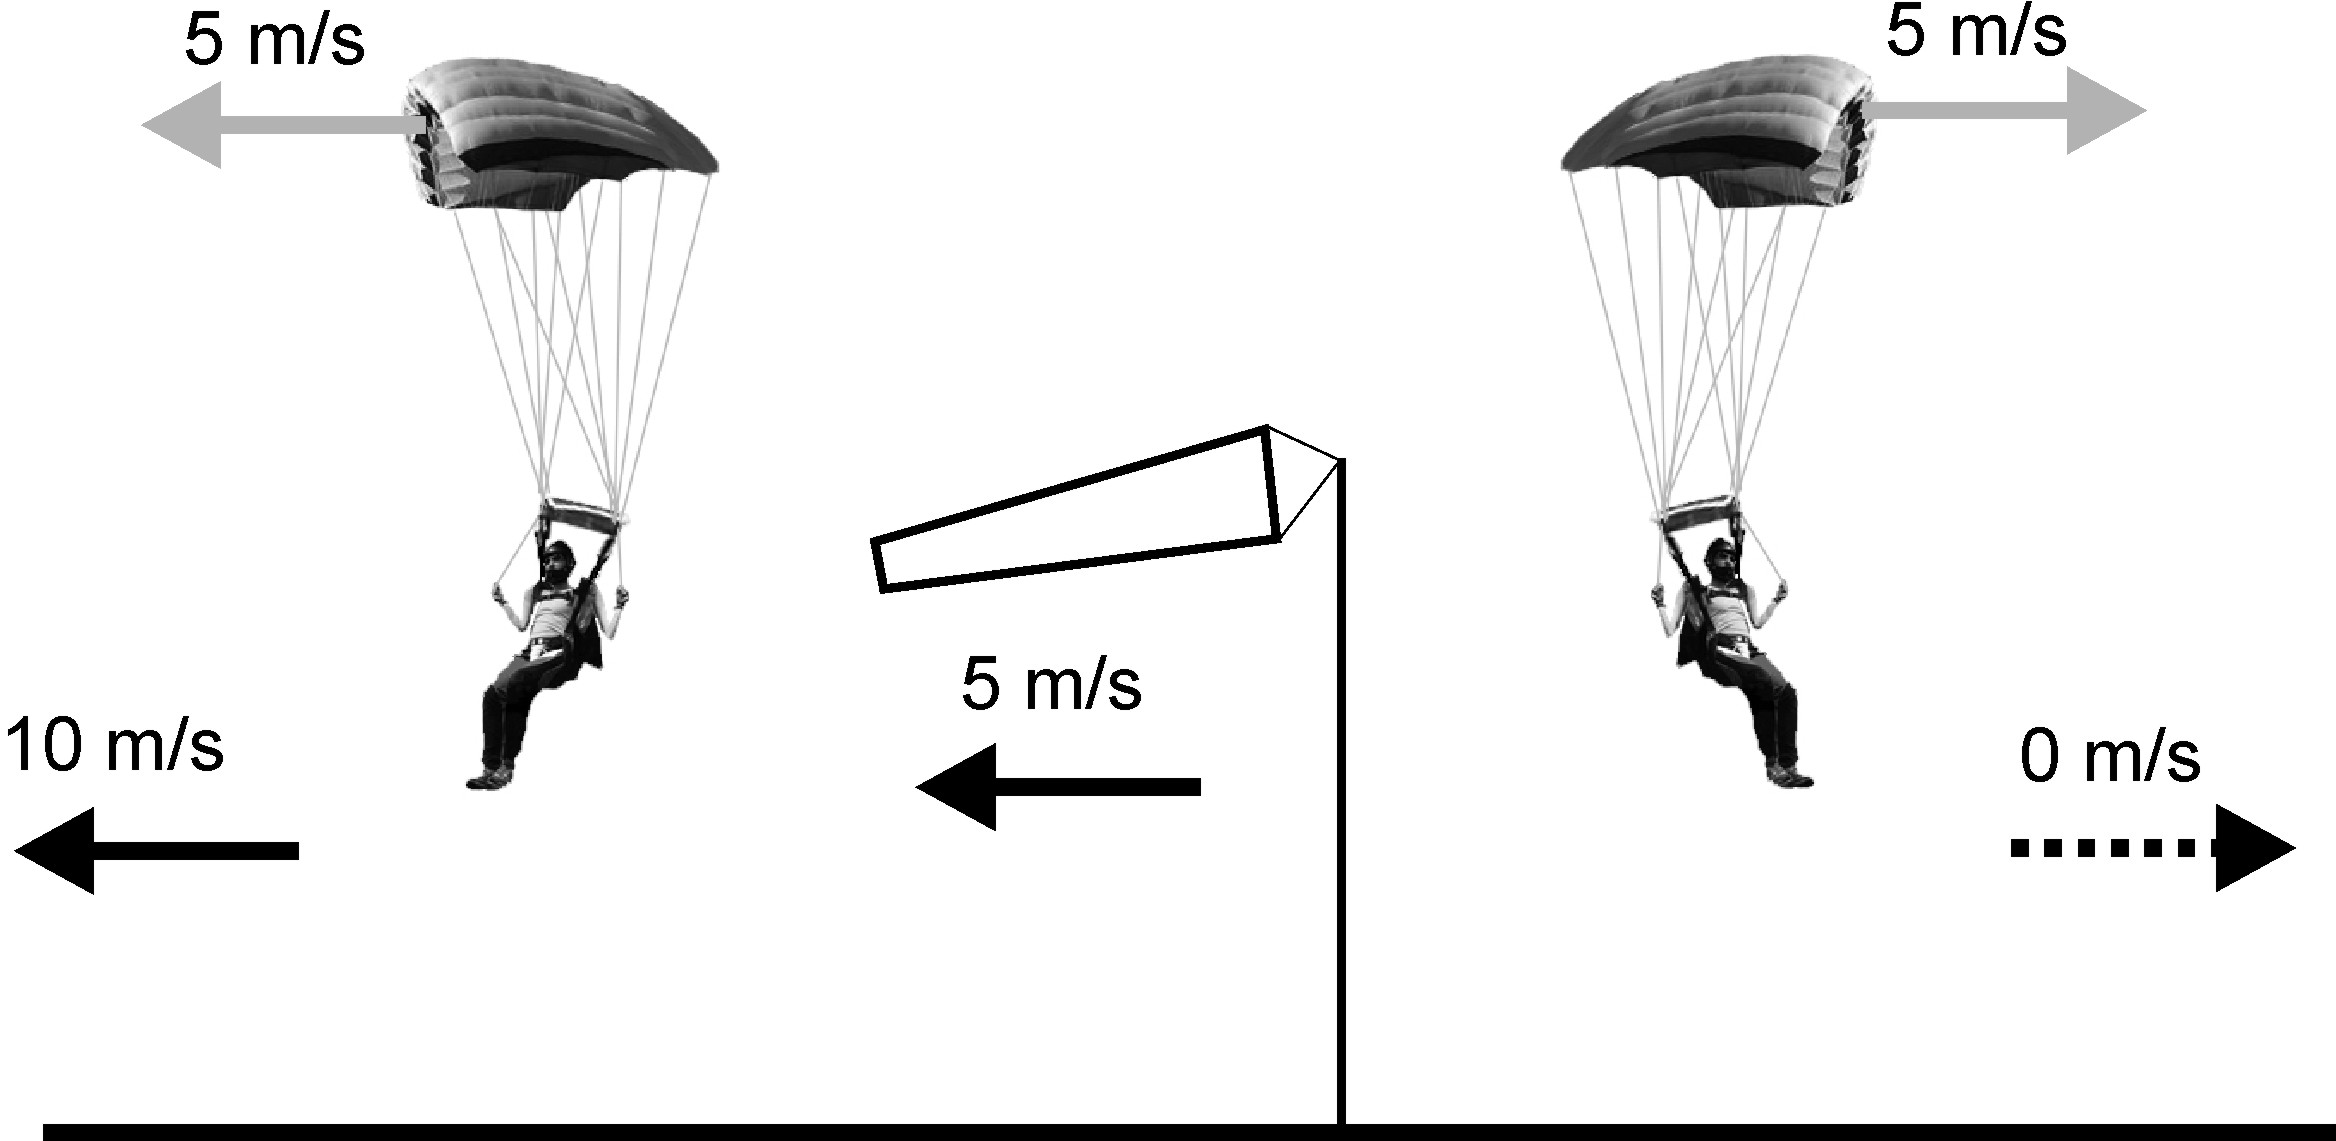
\includegraphics[width=0.7\textwidth]{Ilma-ja-maanopeus.jpeg}\caption{Maanopeus muuttuu riippuen siitä, mihin suuntaan tuuleen nähden lennetään.}\end{figure*} 

\subsection{ Turbulenssi }
\label{hyppytapahtuma-turbulenssi}


\begin{figure*}[]\centering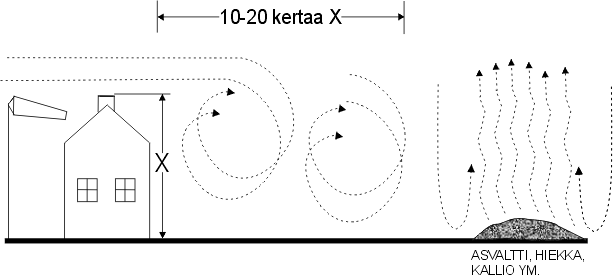
\includegraphics[width=0.7\textwidth]{Turbulenssi.png}\caption{Rakennukset ja lämmin maa aiheuttavat turbulenssia}\end{figure*} 


Turbulenssi ja epätasaiset ilmavirtaukset voivat muuttaa tunneleihin kohdistuvan virtauksen suuntaa siten, että varjo menettää kantokykynsä. Voimakas turbulenssi voi tyhjentää kuvun osittain tai jopa kokonaan. Tyhjentynyt kupu täyttyy uudestaan, kun kupu saavuttaa oikean kohtauskulman ilmavirtaan nähden. Turbulenttinen sää voi estää hyppäämisen, vaikka tuulen voimakkuus ei ylittäisikään oppilastoiminnan tuulirajaa. Jos joudut varjon varassa turbulenssiin, lennä täydessä liidossa. Liian suurilla jarruilla lentäminen saattaa aiheuttaa kuvun sakkaamisen pyörteen vaikutuksesta. 


Pyörre eli turbulenssi voi olla minkä kokoinen tahansa. Pyörteet ovat halkaisijaltaan muutamasta metristä kymmeniin metreihin. Pyörteet syntyvät ilman vapaan virtauksen rikkovista esteistä, kuten rakennuksista, puista, kukkuloista ja maaston lämpötilaeroista (nousevat ja laskevat ilmavirtaukset). Myös toisen laskuvarjon taakse ilmassa muodostuu turbulenssi. 


Hyppääjälle vaarallisimpia ovat yleensä esteistä ja nousevista tai laskevista ilmavirtauksista johtuvat pyörteet. Pyörteitä voi välttää laskeutumalla tarpeeksi kauas esteistä ja esimerkiksi hiekan reunasta, jossa virtausten suunnat muuttuvat. 

\subsection{ Käännökset }
\label{hyppytapahtuma-kaannokset}


Vasemmasta ohjauslenkistä vetämällä varjo kääntyy vasemmalle ja oikeasta vetämällä vastaavasti oikealle. Varjo kallistuu käännöksen suuntaan, joten myös vajoamisnopeus kasvaa. Tämän takia matalalla \textbf{ei saa} tehdä jyrkkiä käännöksiä. 


Käännökset täysliidosta vaativat suuren lentonopeuden takia suuren kääntösäteen. Varjo kallistuu käännöksessä sitä enemmän, mitä enemmän toista ohjauslenkkiä painetaan alaspäin. Tällöin myös vajoaminen kiihtyy. 


Käännökset puolijarrutuksesta tehdään pitämällä toinen ohjauslenkki hartioiden tasalla ja painamalla toista alemmaksi. Varjo kääntyy nopeammin mutta ei kallistu niin paljon. Vajoaminen ei ole niin voimakasta kuin täysliitokäännöksessä. 


Käännökset täysjarrutuksesta tehdään nostamalla vastakkaista ohjauslenkkiä. Varjo reagoi nopeasti ja kallistuu vähemmän kuin muissa lentotiloissa. Täysjarrutustilassa kupu on lähellä sakkaustilaa, joten käännökset on tehtävä hyvin varovasti. 


Mitä suurempi varjon lentonopeus on käännöksessä, sitä suurempi on myös varjon vajoamisnopeus ja kääntösäde. 


Kokeile varjon käyttäytymistä, älä pelkää ohjata sitä. 

\subsection{ Ohjaaminen laskeutumisalueelle }
\label{hyppytapahtuma-ohjaaminen-laskeutumisalueelle}


\begin{figure*}[]\centering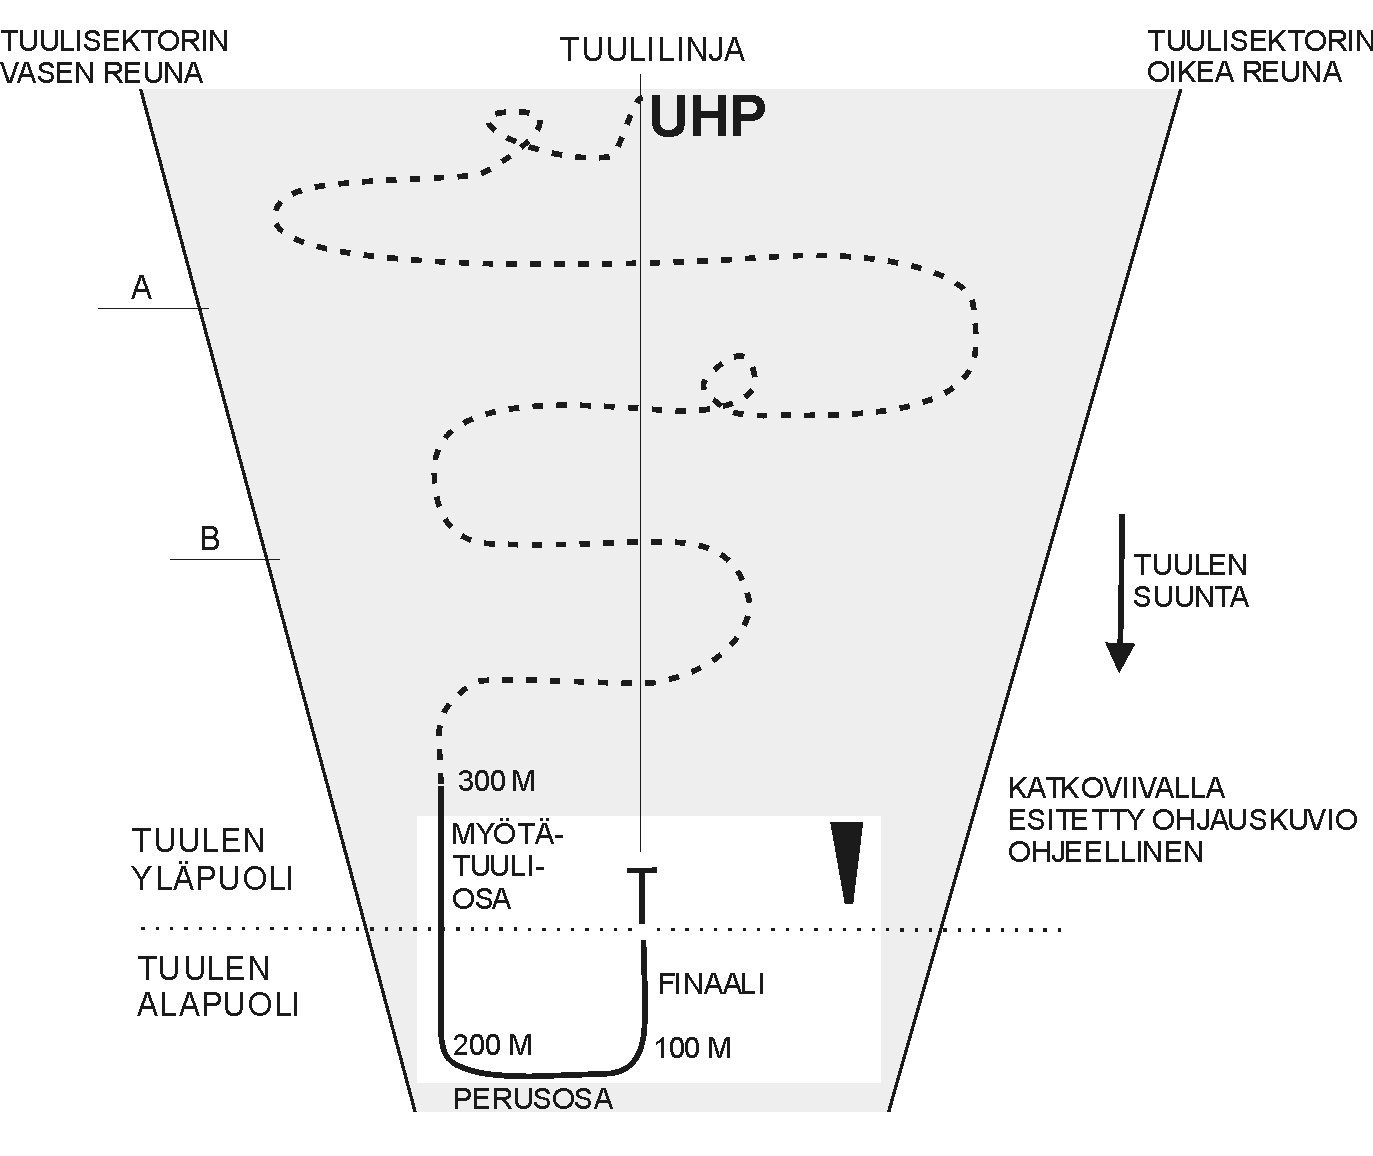
\includegraphics[width=0.5\textwidth]{Tuulisektori.png}\caption{Pysy tuulisektorilla lähestyessäsi laskeutumisaluetta.}\end{figure*} 


Tarkastettuasi ilmatilan, korkeuden, kahvat ja sijainnin aloita ohjaaminen ja käännä varjo tarvittaessa vastatuuleen, jotta pysyt suunnitellulla tuulisektorilla etkä ajaudu liian aikaisin maalialueen lähelle. Vedä mielessäsi viiva nykyisestä paikastasi loppukuvioiden aloituskohtaan ja aseta sille muutama välietappi (kuvassa A ja B). Pudota korkeutta riittävästi ennen seuraavalle välietapille siirtymistä, tarvittaessa lennä hetki vastatuuleen jotta et lähesty sitä liian aikaisin. Selvitä myös sektorin sivurajat, joita et ylitä. Kokeile tämän jälkeen varjon käyttäytymistä eri lentotiloissa: täysliito, puolijarrutus, täysjarrutus ja käännökset. Harjoittele myös loppuvetoa. Lähesty laskeutumisaluetta ottaen huomioon tuuliolosuhteet ja em. lähestymispisteet. Viimeisen 300 metrin matkalla suoritat laskeutumiskuvion, johon kuuluu kolme osaa: myötätuuliosa, perusosa ja finaali. Säännöllisin osuus on finaali, muut osuudet riippuvat tuuliolosuhteista. Tuulisektori on ilmatilakaistale, jossa pysymällä pääset laskeutumaan maalialueelle. Se sijaitsee tuulilinjan molemmin puolin. Oikean uloshyppypaikan ja maalipisteen välinen linja on tuulilinja, pysy sen läheisyydessä. Mitä lähempänä maalialuetta lennetään, \mbox{sitä kapeampi on tuulisektori.} 


\subsection{ Laskeutumiskuvio }
\label{hyppytapahtuma-laskeutumiskuvio}


Laskeutumiskuvio kannattaa lentää varjo puolijarrutuksessa. Puolijarrutustilassa lennettäessä maanopeus on pienempi, varjo kääntyy nopeammin sekä vajoaa käännöksissä vähemmän kuin täysliidossa. 


Myötätuuliosa aloitetaan 300 metrin korkeudessa tuulen yläpuolelta (aloituspiste riippuu tuulen voimakkuudesta). Myötätuuliosa lennetään tuulen alapuolelle noin 100 metriä maalipisteen sivussa. Tuulen alapuolelle lennettävä matka riippuu maatuulen voimakkuudesta.  


Perusosa on sivutuuleen lennettävä osuus. Myötätuuliosalta käännytään perusosalle noin 200 metrin korkeudella. Perusosalla lennetään suoraan maalipisteen taakse tuulen alapuolella. Mitä kovempi tuuli on, sitä enemmän on pidettävä varjoa kääntyneenä vastatuulen suuntaan päästäkseen perusosalla maahan nähden suoraan sivutuuleen. Jos aloitat perusosan liian matalalla, voit oikaista reittiäsi niin, että finaali jää lyhyemmäksi. Vastaavasti, jos aloitat perusosan liian korkealla, voit koukata hieman kauempaa jotta saat aloitettua finaalin haluamassasi pisteessä. 


\begin{Figure}\centering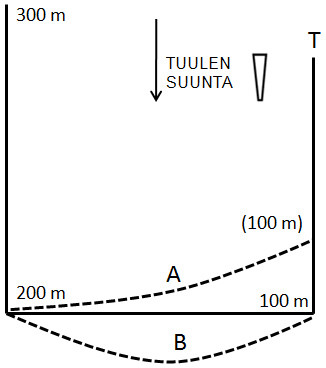
\includegraphics[width=0.8\textwidth]{Laskeutumiskuvio.png}\captionof{figure}{Jos ollaan liian matalalla, voidaan lentää reittiä A. Jos korkeutta on liikaa, voidaan lentää reittiä B.}\end{Figure} 


Vastatuuliosa eli finaali aloitetaan suoraan maalipisteen takaa tuulen alapuolelta. Aloituspiste muuttuu tuulen voimakkuudesta riippuen. Kovalla tuulella finaalin aloituspiste on lähempänä maalipistettä. Finaaliin, joka siis lennetään vastatuuleen, käännytään 100 metrin korkeudessa. Varjo saattaa pyrkiä kääntymään, joten sitä tulee \textbf{ohjata maahan asti}, jotta se pysyisi tarkasti vastatuulessa.  


Jos huomaat lentäväsi finaalissa myötätuuleen, älä käänny vastatuuleen vaan \textbf{laskeudu myötätuuleen}. Myötä- tai sivutuuleen laskeutuminen on turvallisempaa kuin käännöksessä maahan osuminen! 


S-mutkia koko laskeutumiskuvion aikana tulee välttää. Lennä niin, että muut pystyvät ennakoimaan lentoratasi. Tarkkaile ilmatilaa myös laskeutumiskuviossa. 

\begin{verbatim}        
\end{verbatim}

\begin{Figure}\centering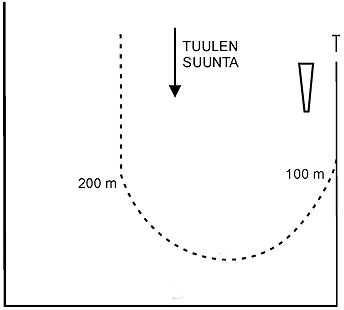
\includegraphics[width=0.8\textwidth]{Laskeutumiskuvio-kovatuuli.png}\captionof{figure}{Kovalla tuulella myötätuuliosuus aloitetaan kauempaa ja loppukuviot lennetään lähempänä maalia. Perusosa jää lyhyemmäksi. (katkoviiva)}\end{Figure} 

\subsection{Laskeutumisen tärkeysjärjestys}
\label{hyppytapahtuma-laskeutumisen-tarkeysjarjestys}

\begin{framed}
\begin{enumerate}[label=\bfseries \arabic*)]
\item  \textbf{Suora finaali} (tärkeintä on, ettei varjo ole laskeuduttaessa käännöksessä) 
\item  Tee \textbf{loppuveto} aina vähintään puolijarrutustilaan 
\item  Pyri laskeutumaan \textbf{vastatuuleen}, esteettömälle alueelle 
\end{enumerate}
\end{framed}

Muista aina laskeutumisen tärkeysjärjestys, se auttaa sinua laskeutumaan turvallisesti! 

\subsection{ Loppuveto ja maahantulo  }
\label{hyppytapahtuma-loppuveto-ja-maahantulo}


Ollessasi finaalissa noin 50 metrin korkeudessa ota hyvä alastuloasento: 

\begin{itemize}
\item  Kädet ohjauslenkeissä 
\item  Leuka kiinni rinnassa ja hampaat yhdessä 
\item  Polvet joustavasti hiukan koukussa ja \textbf{tiukasti} yhdessä 
\item  Jalkaterät 45° etenemissuunnasta sivulle ja \textbf{tiukasti} yhdessä 
\item  Jalkapohjat samalla tasolla ja maanpinnan suuntaiset. 
\end{itemize}

\begin{Figure}\centering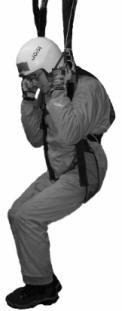
\includegraphics[width=0.5\textwidth]{Alastuloasento.jpeg}\captionof{figure}{Alastuloasento ennen loppuvetoa}\end{Figure} \begin{figure*}[]\centering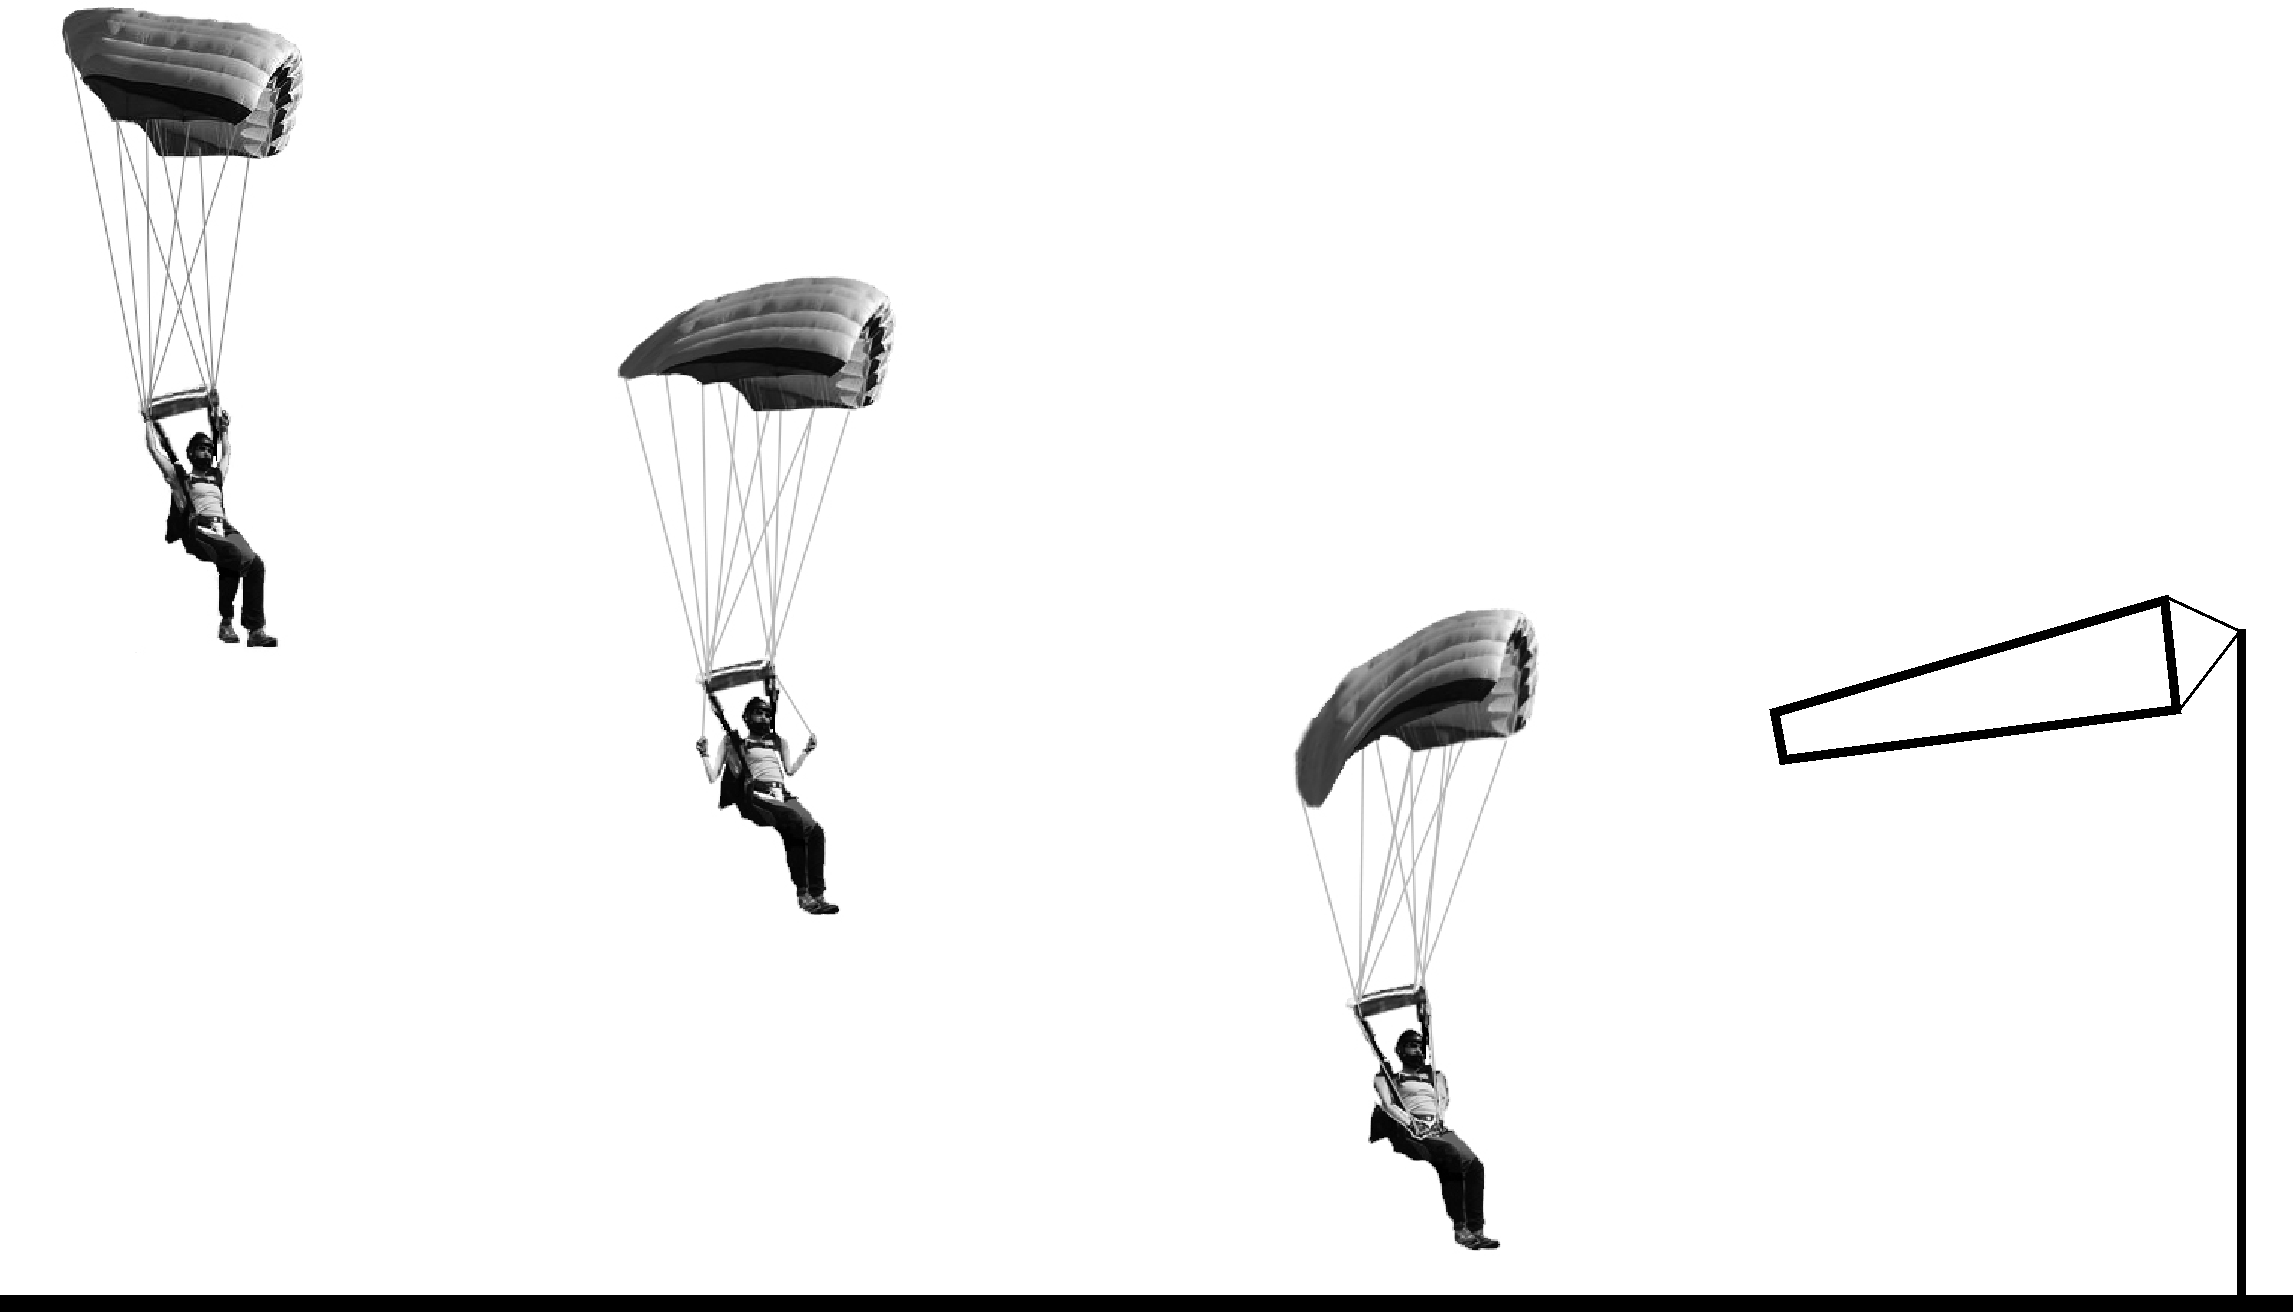
\includegraphics[width=0.6\textwidth]{Loppuveto.png}\caption{Loppuveto}\end{figure*} 


Samalla kun otat alastuloasennon, siirrä ohjauslenkit korvien tasalle. Kun korkeutta on 2-3 metriä, tee loppuveto painamalla ohjauslenkit terävästi täysjarrutustilaan. Ensimmäisillä kolmella hypyllä sinulla on radio, josta kuulet ohjeita esimerkiksi seuraavasti: 

\begin{itemize}
\item  1. hyppy - ohjeita ohjailuun ja laskeutuminen ohjatusti 
\item  2. hyppy - ohjeet tarvittaessa ja laskeutuminen ohjatusti 
\item  3. hyppy - ohjeet vain tarvittaessa 
\end{itemize}

Kun olet noin puiden latvojen tasolla, maa näyttää hyökkäävän silmille. Älä säikähdä, vaan keskity oikeaan alastuloasentoon ja loppuvedon oikeaan ajoitukseen. Korkeuden arvioinnissa voit käyttää apuna esimerkiksi tuulipussin tolppaa, rakennuksen kattoa tai maalialueella olevia ihmisiä.  


Jos teet loppuvedon liian aikaisin ja varjo pysähtyy liian korkealle, \textbf{pidä ohjauslenkit täysjarrutustilassa.} Valmistaudu maahantulokierähdykseen. Jos nostat ohjauslenkit uudelleen ylös, varjo hyökkää eteenpäin ja tulet kovaa maahan. Mikäli et kuule loppuvetokomentoa, niin tee loppuveto itsenäisesti. Jos loppuvedon ajoitus on väärä tai se tehdään huonosti, voi maahantulo olla kova. Tämän vuoksi \textbf{valmistaudu aina tekemään maahantulokierähdys.} 


Suurin osa oppilaiden loukkaantumisista on nilkan nyrjähdyksiä tai murtumia, joista valtaosa olisi vältettävissä hyvän alastuloasennon pitämisellä loppuun saakka. 


Muista aina varjon varassa: 

\begin{itemize}
\item  Tarkkaile ilmatilaa 
\item  Tarkkaile korkeutta 
\item  Vältä rajuja ohjausliikkeitä 
\item  Tarkkaile sijaintiasi ja pysy ohjeistetulla alueella ja suunnitellulla reitillä 
\item  Älä lennä toisen hyppääjän lähellä 
\item  Alempana olevalla on etuajo-oikeus 
\item  Varjo ei käänny hetkessä 
\item  Tarkkaile tuulipussia 
\item  Käänny finaaliin 100 metrissä 
\item  Suora finaali 
\item  Ohjaa varjoa maahan saakka. 
\end{itemize}
\subsection{ Varjon tukahduttaminen }
\label{hyppytapahtuma-varjon-tukahduttaminen}


Kun olet laskeutunut, varjo saattaa hiukan kovemmalla tuulella alkaa vetää sinua perässään. Saat varjon tukahtumaan päästämällä irti toisesta ohjauslenkistä ja vetämällä toisesta kupua luoksesi. Samalla voit juosta varjon toiselle puolelle. Tämä kääntää varjoa niin, ettei tuuli enää pääse täyttämään tunneleita. Aivan viimeisenä keinona voit tehdä päävarjon irtipäästön. (\ref{paavarjon-vajaatoiminnot-varavarjon-kaytto} s.\pageref{paavarjon-vajaatoiminnot-varavarjon-kaytto})  


\textbf{Älä jää maahan makaamaan ellet tarvitse apua.} 


Jos näet hyppääjän vaikeuksissa, velvollisuutesi on auttaa häntä. 

\subsection{ Radiokomennot }
\label{hyppytapahtuma-radiokomennot}


Sinulla on mukanasi radio vähintään kolmella ensimmäisellä hypyllä. Radion tarkoituksena on avustaa sinua ohjaamisessa ja loppuvedon oikea-aikaisessa suorittamisessa. Toimi joka hypyllä itsenäisesti, sillä ohjeita annetaan vain tarvittaessa. Radio on vain apuväline, jossa voi esiintyä häiriöitä. 


1. Yhteyskokeilu ennen koneen kuormausta  


KUTSU = \raisedrule[0.0em]{0.5pt} \\  

\begin{itemize}
\item   Kuittaus kättä nostamalla 
\end{itemize}

2. Yhteyskokeilu ilmassa 


KUTSU + HEILUTA JALKOJA 

\begin{itemize}
\item  Kuittaus jalkojen heilutuksella 
\end{itemize}

3. Käännökset 


KUTSU + VASEN, VASEN, SUORAAN 

\begin{itemize}
\item  Käännä niin kauan, kunnes kuuluu komento SUORAAN 
\end{itemize}

4. Jarruttaminen 


KUTSU + JARRUTA, JARRUTA 

\begin{itemize}
\item  Jokaisella komennolla laske ohjauslenkkejä 10-15 cm 
\end{itemize}

5. Jarrutuksen vähentäminen 


KUTSU + NOSTA, NOSTA 

\begin{itemize}
\item  Jokaisella komennolla nosta ohjauslenkkejä 10-15 cm 
\end{itemize}

KUTSU + LIIDÄ 

\begin{itemize}
\item  Täysliito 
\end{itemize}

6. Itsenäinen ohjaaminen 


KUTSU + OHJAA ITSENÄISESTI 

\begin{itemize}
\item  Jatka ohjaamista itsenäisesti. 
\item  Kumoaa edellisten komentojen vaikutuksen. 
\end{itemize}

7. Loppuveto 


KUTSU + JALAT YHTEEN 

\begin{itemize}
\item  Hyvä alastuloasento, jalat tiukasti yhdessä. 
\end{itemize}

VEDÄ 

\begin{itemize}
\item  Paina ohjauslenkit terävästi täysjarrutustilaan, pidä alastuloasento. 
\end{itemize}
\end{multicols}

\chapter{Päävarjon vajaatoiminnot}
\label{paavarjon-vajaatoiminnot}
\thispagestyle{headings}
\begin{multicols}{2}

Varjo ei välttämättä ole aina avautumisen jälkeen täysin kehittynyt vaan vaatii kierteiden poiston ja/tai pumppausta (\ref{hyppytapahtuma-varjon-avautuminen-ja-lentokuntoon-saattaminen} s.\pageref{hyppytapahtuma-varjon-avautuminen-ja-lentokuntoon-saattaminen}). Molemmat ovat aivan normaaleja toimenpiteitä varsinkin pakkolaukaisuhypyillä (syynä esimerkiksi huono uloshyppy tai lentokoneen alhainen ilmanopeus). Varjo lentää, vaikka punoksissa on kierrettä, kuvun reunatunnelit ovat tukossa ja slider on ylhäällä, mikäli varjo täyttää lentävän laskuvarjon kriteerit: 

\begin{framed}
\begin{itemize}
\item  Kupu on säännöllisen muotoinen. 
\item  Punokset ovat kireällä. 
\item  Slider on suorakaiteen muotoinen. 
\end{itemize}
\end{framed}

Muista aina tarkkailla korkeutta, jotta voit tarvittaessa ajoissa suorittaa varavarjotoimenpiteet. 


\textbf{Jos et osaa päättää, lentääkö päävarjo vai ei, se EI LENNÄ!} => Tee varavarjotoimenpiteet! 

\section{ Lentää, Täysin kehittynyt }
\label{paavarjon-vajaatoiminnot-lentaa-taysin-kehittynyt}


\begin{Figure}\centering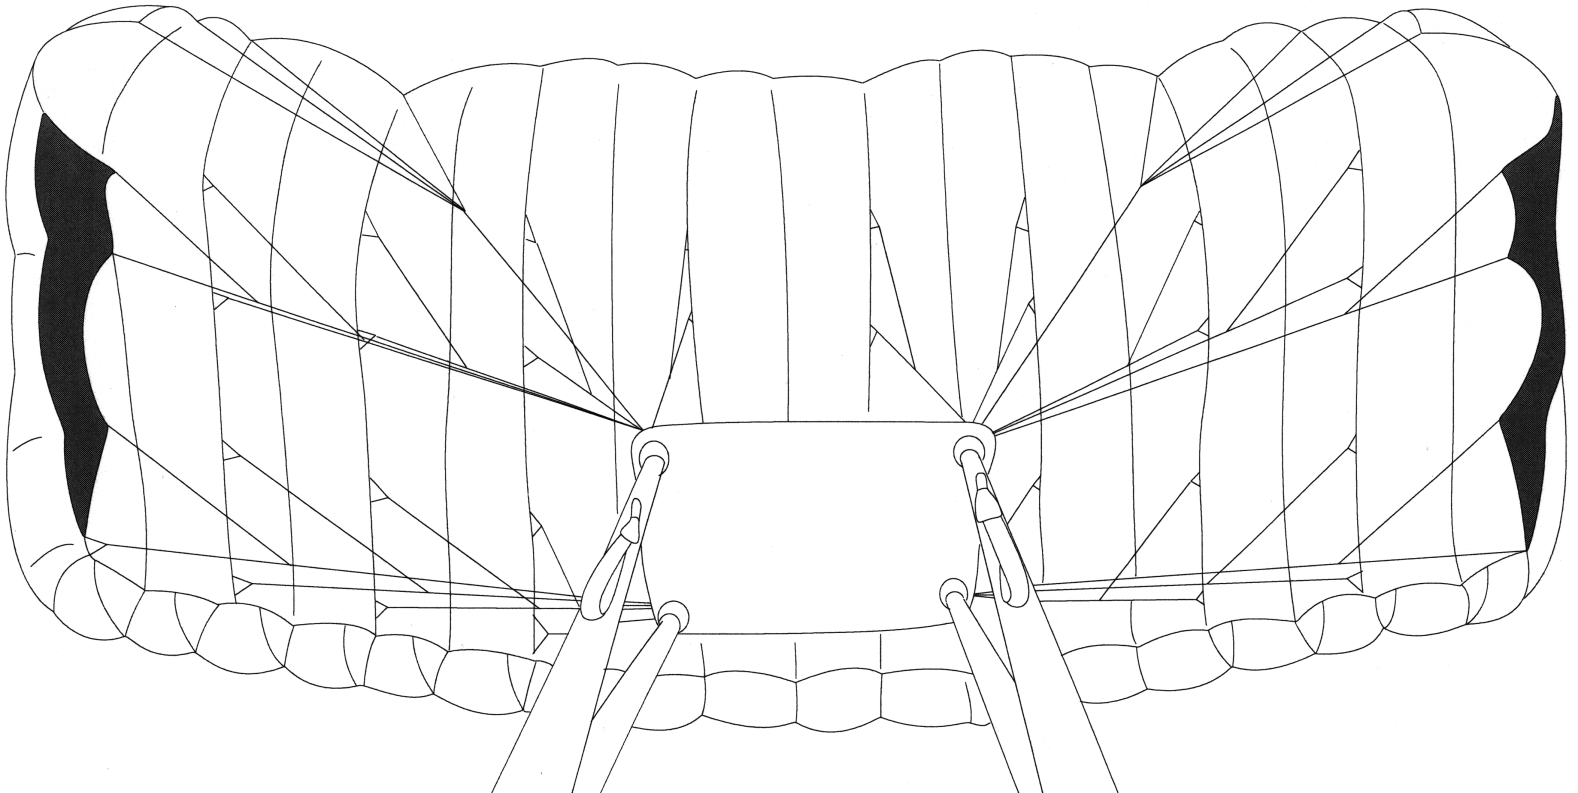
\includegraphics[width=0.95\textwidth]{Vajaatoiminnot-Lentaa-Taysin-kehittynyt.png}\end{Figure} 

\begin{itemize}
\item  Kupu on säännöllisen muotoinen 
\item  Punokset ovat kireällä 
\item  Slider on suorakaiteen muotoinen ja alhaalla. 
\end{itemize}

\section{ Lentää - Selvitä }
\label{paavarjon-vajaatoiminnot-lentaa-selvita}

\subsubsection{Slider ylhäällä}
\label{paavarjon-vajaatoiminnot-slider-ylhaalla}


\begin{Figure}\centering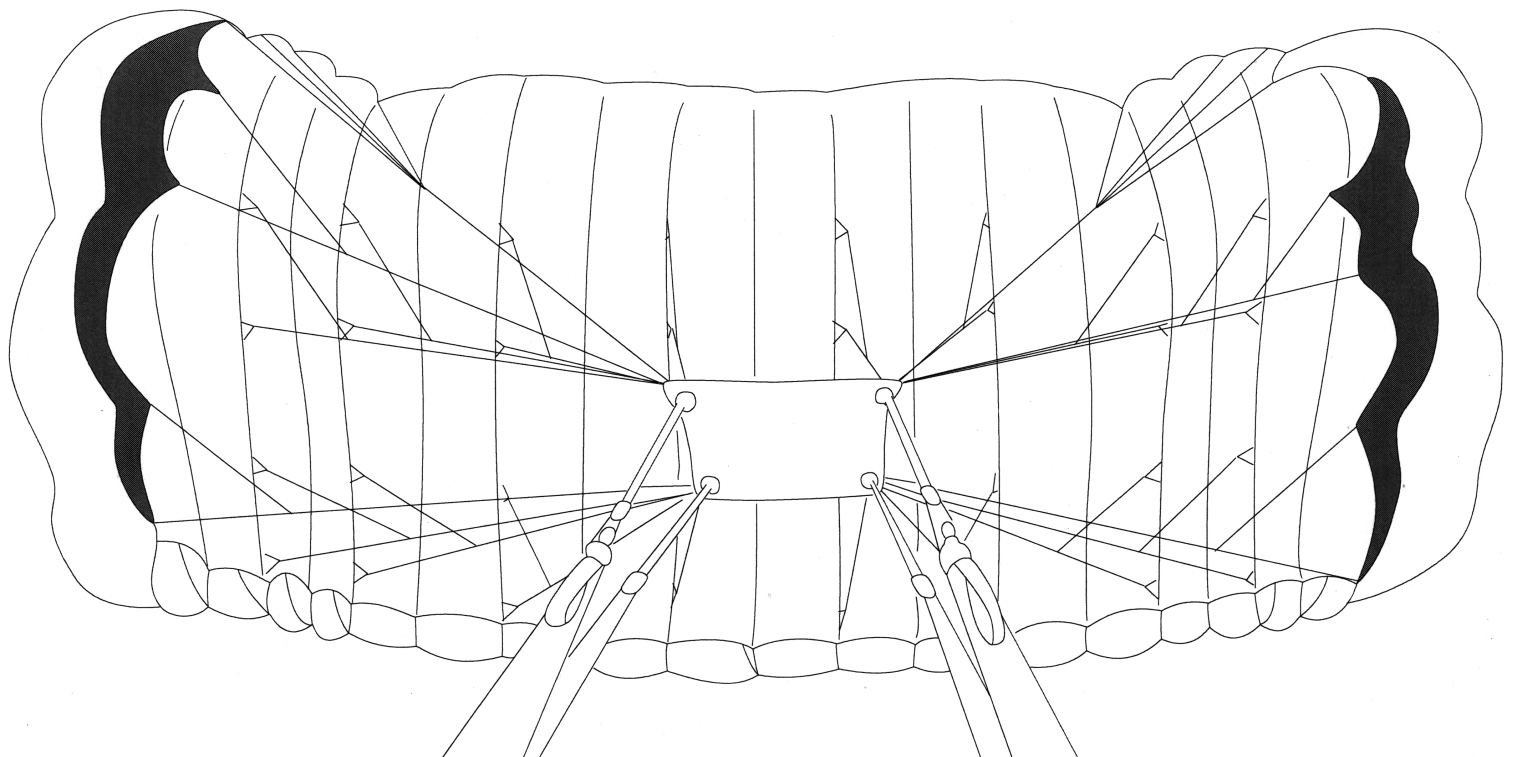
\includegraphics[width=0.95\textwidth]{Vajaatoiminnot-Lentaa-Slider-ylhaalla.png}\end{Figure} 

\begin{itemize}
\item  Pumppaa slider alas 
\item  Tarkkaile korkeutta. 
\end{itemize}
\subsubsection{Slider ylhäällä ja kierrettä}
\label{paavarjon-vajaatoiminnot-slider-ylhaalla-ja-kierretta}


\begin{Figure}\centering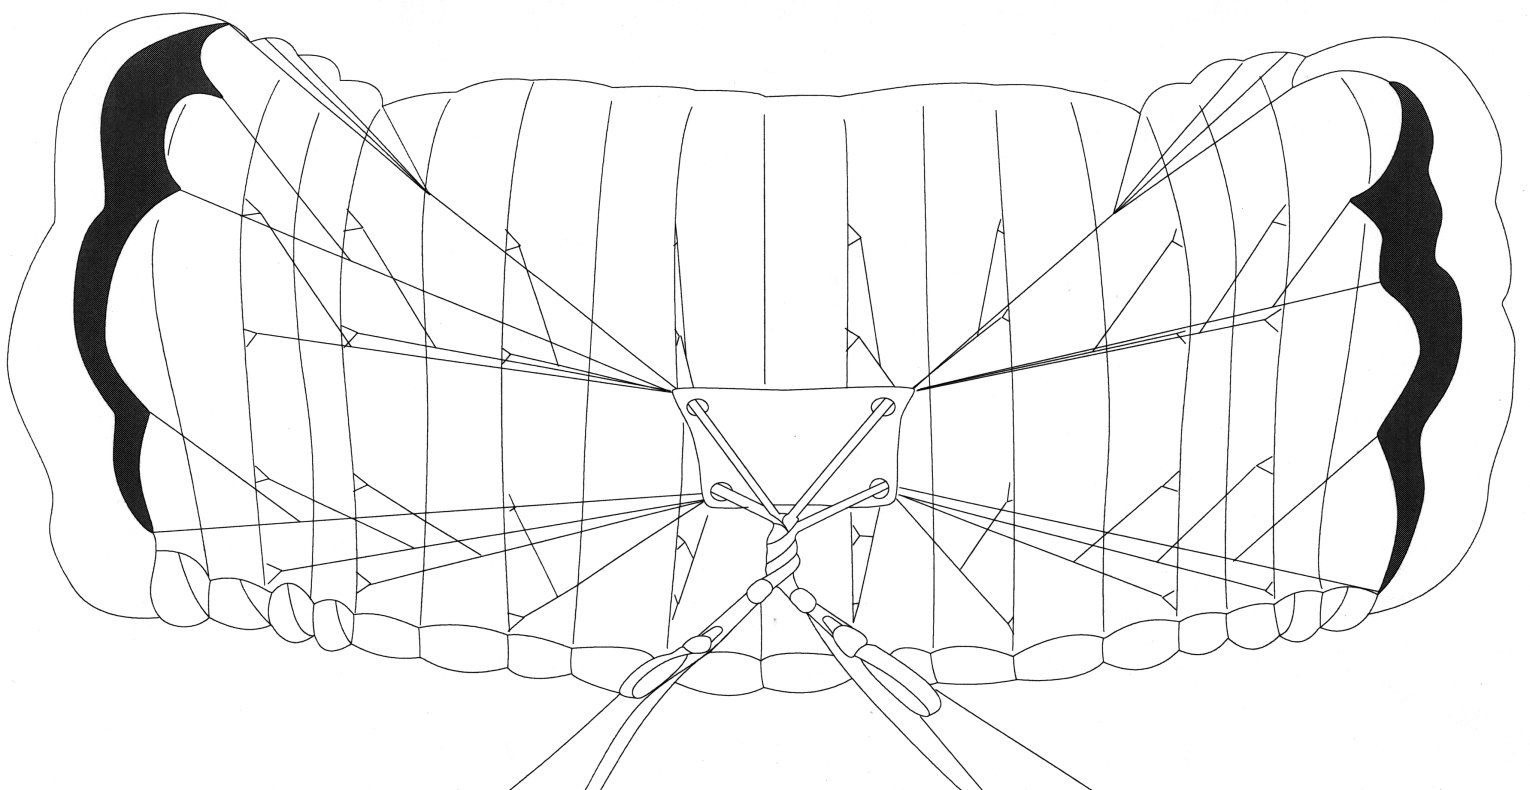
\includegraphics[width=0.95\textwidth]{Vajaatoiminnot-Lentaa-Slider-ylhaalla-ja-Kierteita.png}\end{Figure} 

\begin{itemize}
\item  Levitä kantohihnoja, potki kierre auki ja pumppaa slider alas 
\item  Tarkkaile korkeutta. 
\end{itemize}
\subsubsection{Reunatunnelit tukossa ja slider ylhäällä}
\label{paavarjon-vajaatoiminnot-reunatunnelit-tukossa-ja-slider-ylhaalla}


\begin{Figure}\centering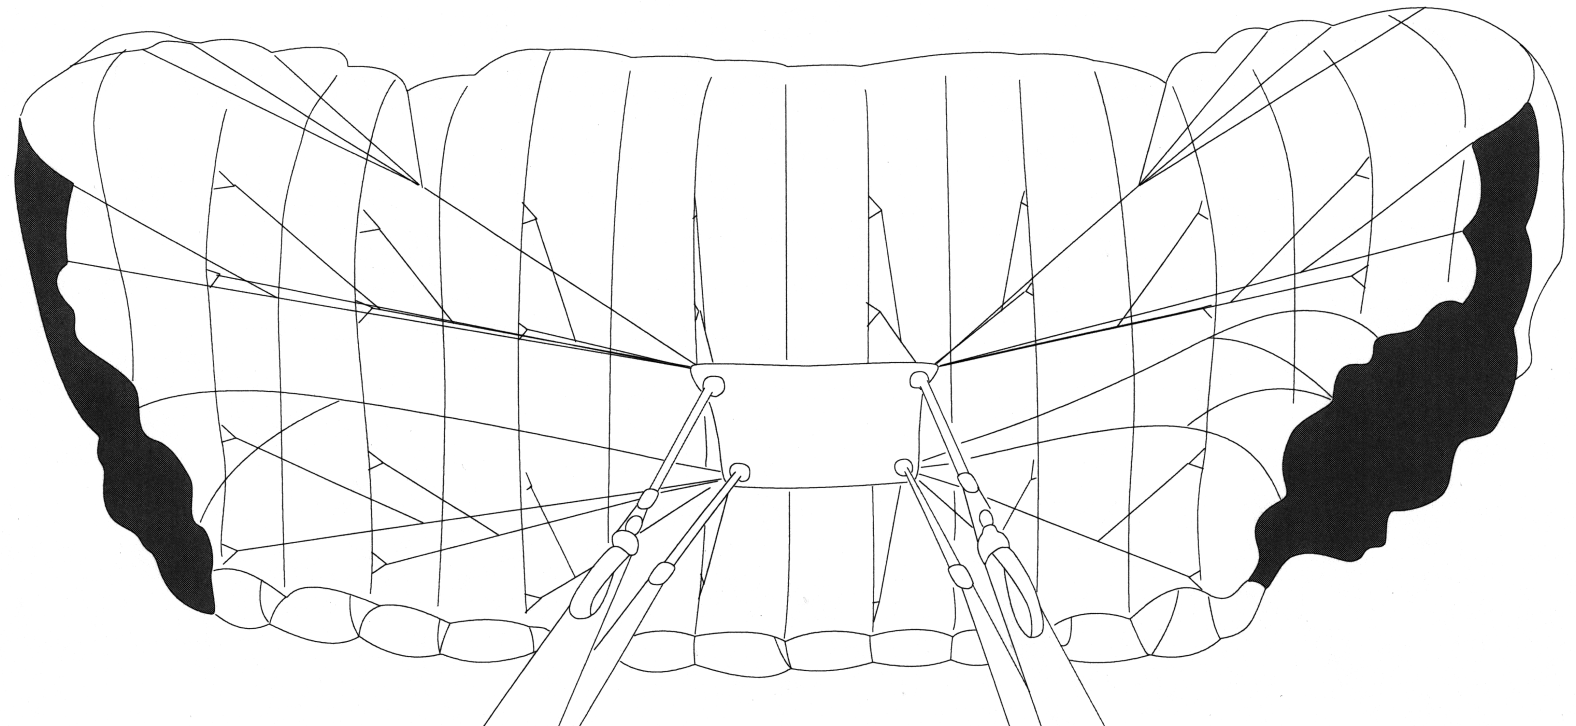
\includegraphics[width=0.95\textwidth]{Vajaatoiminnot-Lentaa-Reunatunnelit-tukossa-ja-slider-ylhaalla.png}\end{Figure} 

\begin{itemize}
\item  Pumppaa slider alas ja tunnelit auki 
\item  Tarkkaile korkeutta. 
\end{itemize}
\subsubsection{Reunatunneli tukossa, slider ylhäällä ja kierrettä punoksissa}
\label{paavarjon-vajaatoiminnot-reunatunneli-tukossa-slider-ylhaalla-ja-kierretta-punoksissa}


\begin{Figure}\centering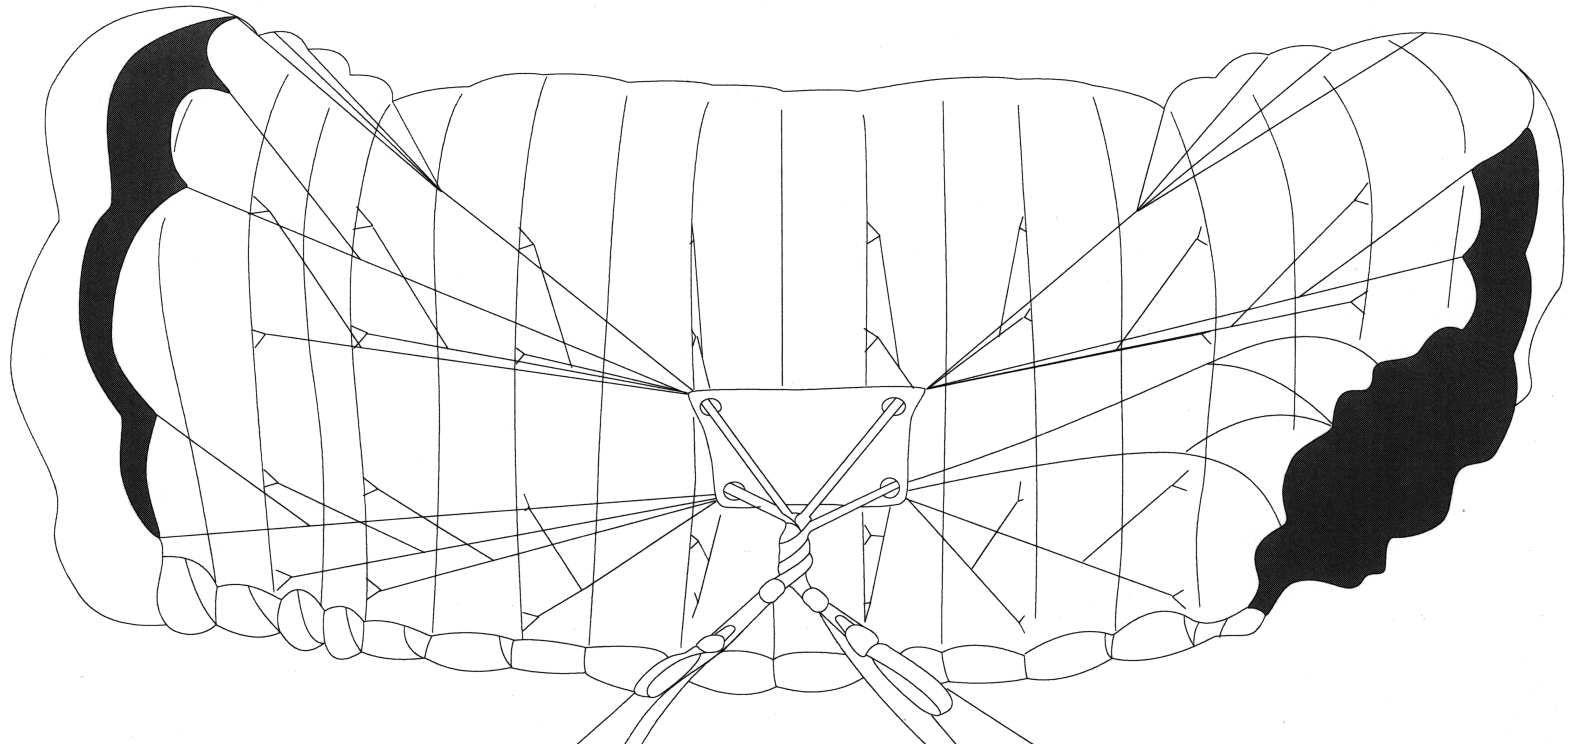
\includegraphics[width=0.95\textwidth]{Vajaatoiminnot-Lentaa-Reunatunnelit-tukossa-ja-slider-ylhaalla-ja-kierteita.png}\end{Figure} 

\begin{itemize}
\item  Levitä kantohihnoja, potki kierre auki, pumppaa slider alas ja tunneli auki 
\item  Tarkkaile korkeutta. 
\end{itemize}
\subsubsection{Avautumassa oleva varjo}
\label{paavarjon-vajaatoiminnot-avautumassa-oleva-varjo}


\begin{Figure}\centering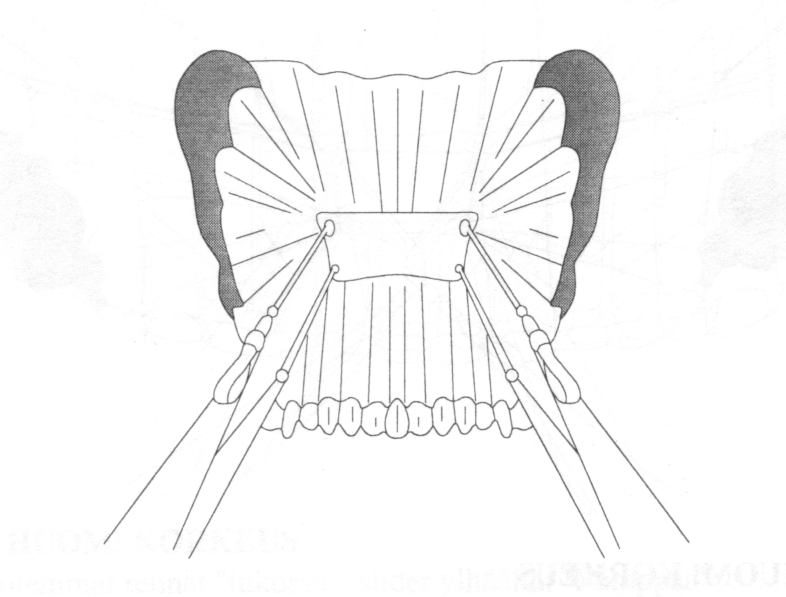
\includegraphics[width=0.95\textwidth]{Vajaatoiminnot-lentaa-avautumassa.png}\end{Figure} 

\begin{itemize}
\item  Pumppaa kupu tarvittaessa auki 
\item  Tarkkaile korkeutta. 
\end{itemize}
\section{ Ei lennä }
\label{paavarjon-vajaatoiminnot-ei-lenna}

\subsubsection{Line over}
\label{paavarjon-vajaatoiminnot-line-over}


\begin{Figure}\centering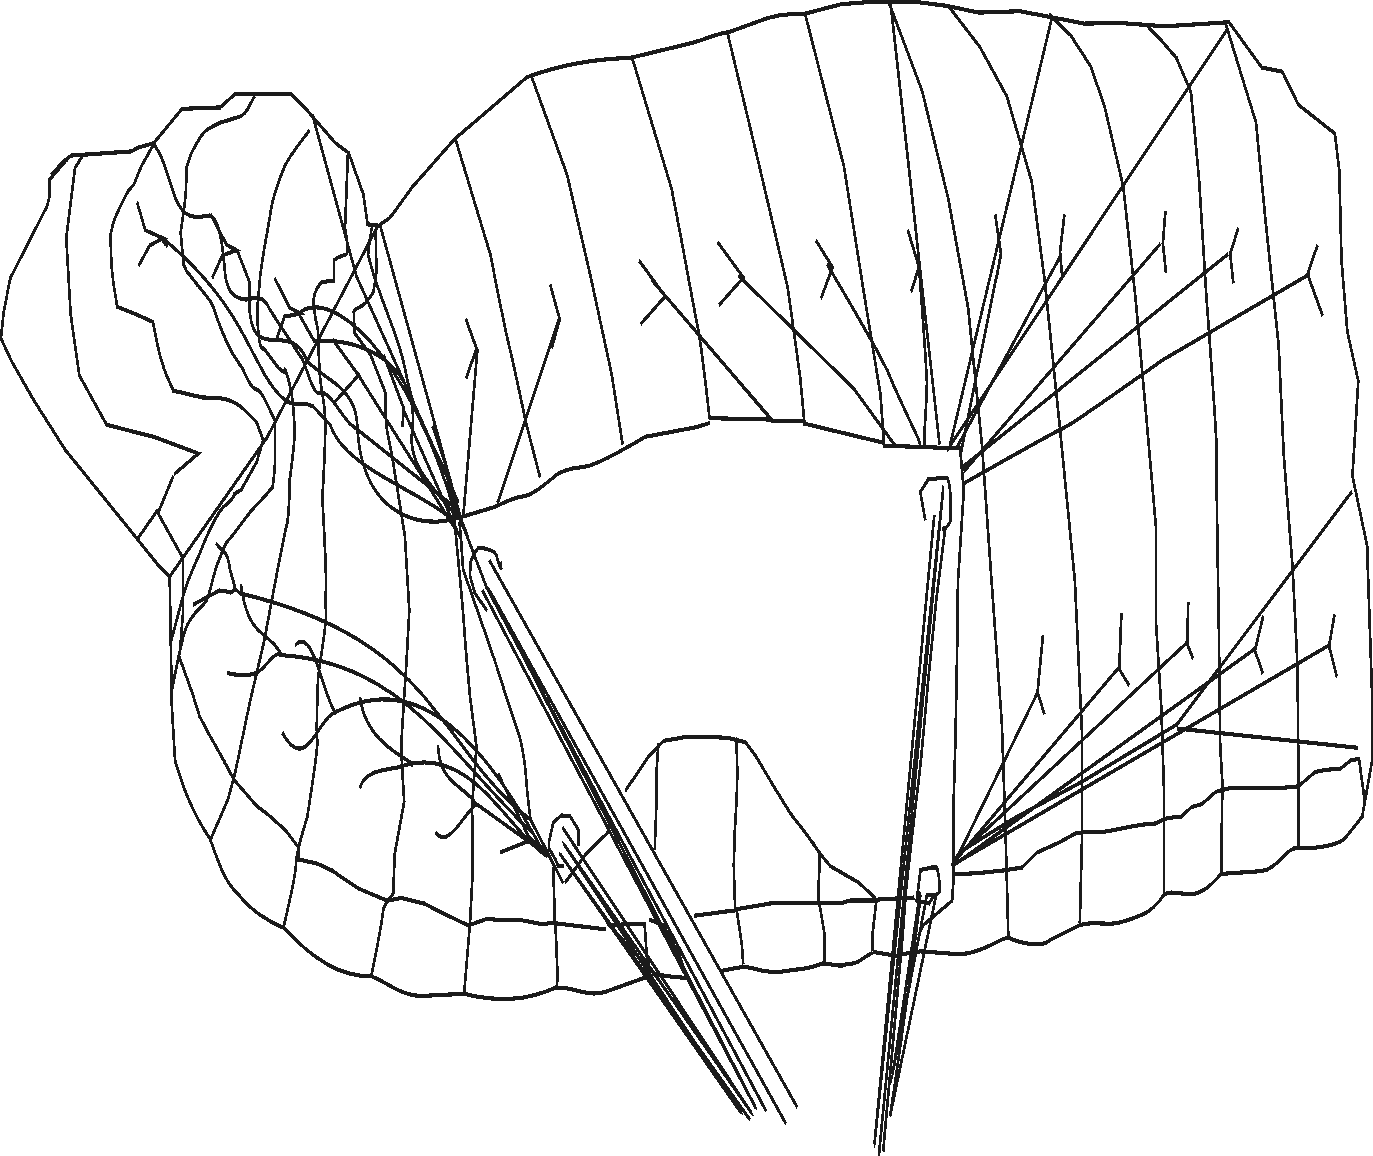
\includegraphics[width=0.95\textwidth]{Vajaatoiminnot-line-over.png}\end{Figure} 

\begin{itemize}
\item  Tee varavarjotoimenpiteet. 
\end{itemize}

\begin{figure*}[]\centering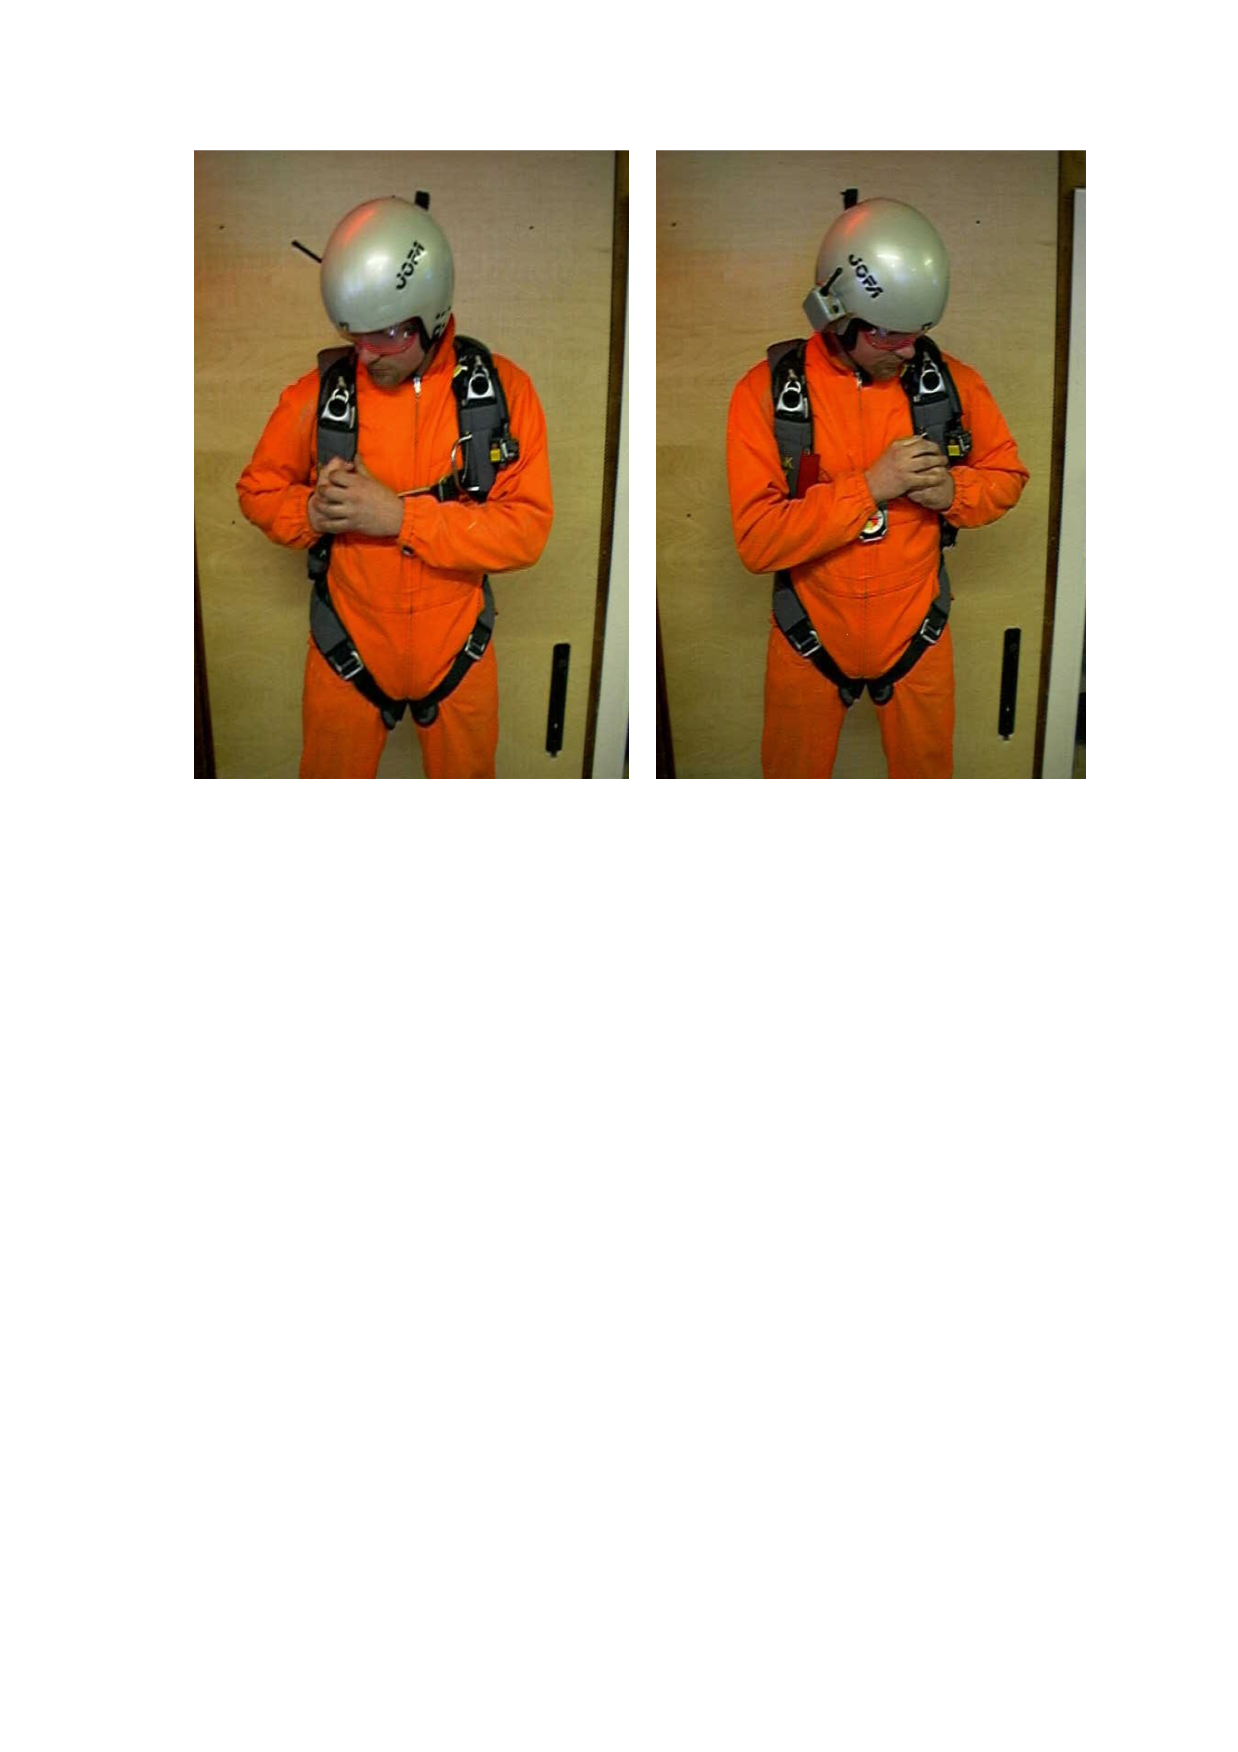
\includegraphics[width=0.8\textwidth]{VV-toimenpiteet.pdf}\caption{VV-toimenpiteet}\end{figure*} 

\begin{verbatim} 
\end{verbatim}
\section{ Varavarjon käyttö }
\label{paavarjon-vajaatoiminnot-varavarjon-kaytto}


Tärkeät korkeudet: 

\begin{description}
\item[ 600 m ] \hfill \\ 
	\begin{itemize}
	\item  Tähän asti voit selvittää päävarjoa eli poistaa kierteitä, pumpata slideriä alas ja reunatunneleita auki. 
	\item  Jos yritykset eivät onnistu 600 metriin mennessä, tee varavarjotoimenpiteet. 
	\end{itemize}
\item[ 300 m ] \hfill \\ 
	\begin{itemize}
	\item  Tämän korkeuden alapuolella ei suositella päävarjon irtipäästöä (esimerkiksi törmättyäsi toiseen hyppääjään (\ref{mahdolliset-vaaratilanteet-tormaaminen-varjon-varassa} s.\pageref{mahdolliset-vaaratilanteet-tormaaminen-varjon-varassa})), sillä varavarjo ei välttämättä ehdi avautua. Mikäli joudut tilanteeseen, jossa sinulla on korkeutta alle 300 metriä ja päävarjosi ei lennä, avaa suoraan varavarjo tekemättä päävarjon irtipäästöä (kohdat 6-9 alla). 
	\end{itemize}
\end{description}
\subsubsection{ Varavarjotoimenpiteet }
\label{paavarjon-vajaatoiminnot-varavarjotoimenpiteet}

\begin{enumerate}[label=\bfseries \arabic*)]
\item  Pidä taivutus. 
\item  Tarkasta korkeus. 
\item  Katso päävarjon irtipäästöpampulaa (oikealla) ja ota siitä kiinni molemmin käsin. 
\item  Murra tarra ja vedä kädet suoriksi alaviistoon.  
\item  Päästä pampulasta irti 
\item  Katso varavarjon kahvaa (vasemmalla) ja ota siitä kiinni molemmin käsin. 
\item  Murra tarra ja vedä kädet suoriksi alaviistoon. 
\item  Taivuta. 
\item  Pidä vv-kahva kädessä tai päästä irti (kerhokohtainen) 
\end{enumerate}

\begin{figure*}[]\centering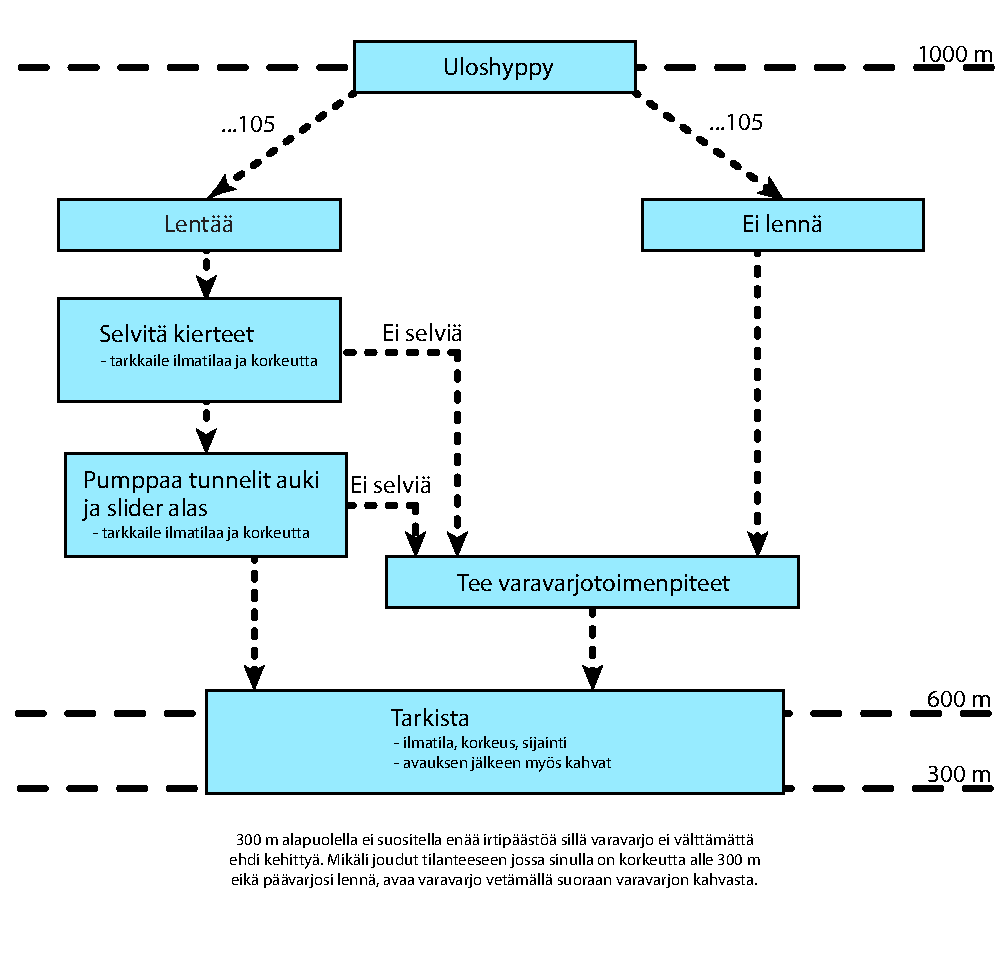
\includegraphics[width=0.99\textwidth]{VVkaavio.pdf}\caption{Toiminta päävarjon vajaatoiminnoissa}\end{figure*} 

\end{multicols}

\chapter{Mahdolliset vaaratilanteet}
\label{mahdolliset-vaaratilanteet}
\thispagestyle{headings}
\begin{multicols}{2}
\section{ Vaaratilanteet koneessa ja uloshypyssä }
\label{mahdolliset-vaaratilanteet-vaaratilanteet-koneessa-ja-uloshypyssa}

\subsection{ Repun aukeaminen koneessa }
\label{mahdolliset-vaaratilanteet-repun-aukeaminen-koneessa}


Repun (pää- tai varavarjon) tahaton aukeaminen johtuu yleensä hyppääjän varomattomasta liikkumisesta. Reppu, varavarjon kahva tai päävarjon aukaisujärjestelmä voivat tarttua jonnekin kiinni. Rauhallinen, tarpeettomia liikkeitä välttävä liikkuminen ehkäisee tarttumistilanteita tehokkaasti. Jos oma tai jonkun muun reppu kuitenkin aukeaa, estetään varjon avautuminen sekä ilmoitetaan asiasta hyppymestarille. 


Koneen lentäessä ovi auki on mahdollista, että reppu aukeaa ja varjo joutuu ilmavirtaan. Jos varjo purkautuu koneen sisällä ja ilmavirta tarttuu siihen, varjo voi vetää hyppääjän ulos. Tällaisessa tilanteessa sekä lentokone että hyppääjä voivat vahingoittua.  


Jos reppusi aukeaa ovella ja varjo karkaa ovesta ulos, hyppää ulos asennosta välittämättä. Tällaisessa tapauksessa hyppymestari auttaa sinut ripeästi ulos. Nopealla toiminnalla tilanne voidaan pelastaa. 

\subsection{ Hätähyppy }
\label{mahdolliset-vaaratilanteet-hatahyppy}


Jos lentäjän täytyy keventää konetta tai kone on ohjauskyvytön, hyppymestari antaa hyppääjille komennon HÄTÄHYPPY!  Komennolla OVELLE! siirrytään etuilematta ovelle ja komennolla MENE! poistutaan välittömästi. Hätähyppyä jatketaan, kunnes kaikki ovat hypänneet tai hyppymestari komentaa SEIS, PAKKOLASKU! Tällöin loput koneessa olevat valmistautuvat pakkolaskuun. 

\subsection{ Pakkolasku }
\label{mahdolliset-vaaratilanteet-pakkolasku}


Hyppytoiminnassa lennetään yleensä niin lähellä kenttää, että hyppykone pystyy liitämään takaisin esimerkiksi moottorihäiriön sattuessa. Tällöin hyppymestari ilmoittaa asiasta komennolla PAKKOLASKU! Automaattilaukaisin käännetään tällöin OFF-asentoon ja toimitaan ohjeiden mukaan. 


Kun kone on maassa ja pysähtynyt, on tulipalovaaran takia poistuttava nopeasti. Loukkaantuneita autetaan mahdollisuuksien mukaan. Hätähypyssä ja pakkolaskussa on muistettava, että lentäjä on koneen päällikkö mutta hyppääjien johtaja on hyppymestari. Oppilaille ohjeet tulevat \textbf{aina} hyppymestarilta. Tärkeintä on toimia rauhallisesti käskyjen mukaan. 

\subsection{ Koneeseen kiinni jääminen }
\label{mahdolliset-vaaratilanteet-koneeseen-kiinni-jaaminen}


Jos jäät roikkumaan koneeseen päävarjostasi, huomaat sen siitä, että roikut olkalukoista päävarjon kantohihnojen välityksellä. Yritä ottaa taivutettu asento jotta et pyöri ja voit varmistaa mistä olet kiinni. Varmistu, että olet hinauksessa vain olkalukkojen välityksellä jonka jälkeen tee varavarjotoimenpiteet. (\ref{paavarjon-vajaatoiminnot-varavarjon-kaytto} s.\pageref{paavarjon-vajaatoiminnot-varavarjon-kaytto}) 

\section{ Sotkeutuminen punoksiin }
\label{mahdolliset-vaaratilanteet-sotkeutuminen-punoksiin}


Jos uloshyppysi tai avausasentosi on huono, on mahdollista, että sotkeudut punoksiin. Pyri tällöin irrottautumaan takertuneista punoksista ennen varavarjotoimenpiteitä. Käytä tarvittaessa koukkupuukkoa. Tee kuitenkin varavarjotoimenpiteet (\ref{paavarjon-vajaatoiminnot-varavarjon-kaytto} s.\pageref{paavarjon-vajaatoiminnot-varavarjon-kaytto}) viimeistään 600 metrin korkeudessa. Punoksiin sotkeutumisen voi välttää keskittymällä hyvään asentoon ulos hypätessä ja varjoa avatessa. 

\section{ Apuvarjon aiheuttamat vaaratilanteet }
\label{mahdolliset-vaaratilanteet-apuvarjon-aiheuttamat-vaaratilanteet}


Huono avausasento voi johtaa siihen, että apuvarjon yhdyspunos kietoutuu esimerkiksi kätesi ympärille. Ravista kättäsi saadaksesi yhdyspunoksen irti. Jos et saa yhdyspunosta yhdellä yrityksellä irti tai et tiedä mihin se on tarttunut, tee varavarjotoimenpiteet. (\ref{paavarjon-vajaatoiminnot-varavarjon-kaytto} s.\pageref{paavarjon-vajaatoiminnot-varavarjon-kaytto}) Jos yhdyspunos on tarttunut käteesi, voit joutua tekemään varavarjotoimenpiteet yhdellä kädellä. Hyvällä uloshypyllä, avausasennolla sekä apuvarjon kunnollisella heittämisellä vapaaseen ilmavirtaan ehkäiset tehokkaasti edellisen kaltaisia vaaratilanteita. 


Apuvarjo voi avautumistilanteessa joskus tulla kuvun etureunan kautta kuvun alapuolelle. Tee ohjauskokeiluja saadaksesi selville käyttäytyykö varjo normaalisti. Jos varjo ei ohjaudu tai tekee rajuja liikkeitä, tee varavarjotoimenpiteet. (\ref{paavarjon-vajaatoiminnot-varavarjon-kaytto} s.\pageref{paavarjon-vajaatoiminnot-varavarjon-kaytto}) 


Avauksessa apuvarjo voi jäädä hyppääjän selän taakse muodostuvaan pyörteeseen eli turbulenssiin. Jos apuvarjon heiton jälkeen laskettuasi 105:een ei ole tapahtunut mitään, vilkaise olkapään yli (tarkasta). Asento kallistuu ja apuvarjon pitäisi saada ilmaa. Ellei varjo heti avaudu, tee varavarjotoimenpiteet, (\ref{paavarjon-vajaatoiminnot-varavarjon-kaytto} s.\pageref{paavarjon-vajaatoiminnot-varavarjon-kaytto}) koska apuvarjo tai yhdyspunos on saattanut tarttua johonkin kiinni tai reppu on jumissa. Kiinni tarttunutta osaa voidaan yrittää irrottaa, jos varmuudella nähdään ongelman aiheuttaja. Jos irrotus ei onnistu yhdellä yrityksellä tai et näe ongelman aiheuttajaa, tee varavarjotoimenpiteet heti. 

\section{ Vaaratilanteet varjon varassa }
\label{mahdolliset-vaaratilanteet-vaaratilanteet-varjon-varassa}

\subsection{ Kaksi varjoa auki }
\label{mahdolliset-vaaratilanteet-kaksi-varjoa-auki}


Yleisimmät syyt oppilailla kahden varjon varaan joutumisessa ovat matala avaus (itseaukaisuhypyillä), automaattilaukaisimen toimintahäiriö tai liian raju varjon käsittely (mm. poraaminen tai sakkaaminen). Kahden varjon tilanteissa ei lennetä laskeutumiskuviota. Mikäli toisen varjon puolijarrut ovat auki, pidä varjojen nopeus samana sopivilla jarruasetuksilla. 

%% Kahden liitovarjon yhdistelmä voi asettua erilaisiin muodostelmiin, jos molemmat varjot lentävät: 

\subsubsection{ Varjot peräkkäin (biplane) }
\label{mahdolliset-vaaratilanteet-varjot-perakkain-biplane}


Ohjaa varovasti etummaista varjoa vain välttämättömillä ohjausliikkeillä takimmaisista kantohihnoista. Älä avaa puolijarruja. Älä jarruta alastulossa ja valmistaudu kovaan alastuloon. 


\textbf{Älä päästä päävarjoa irti!} 


\begin{Figure}\centering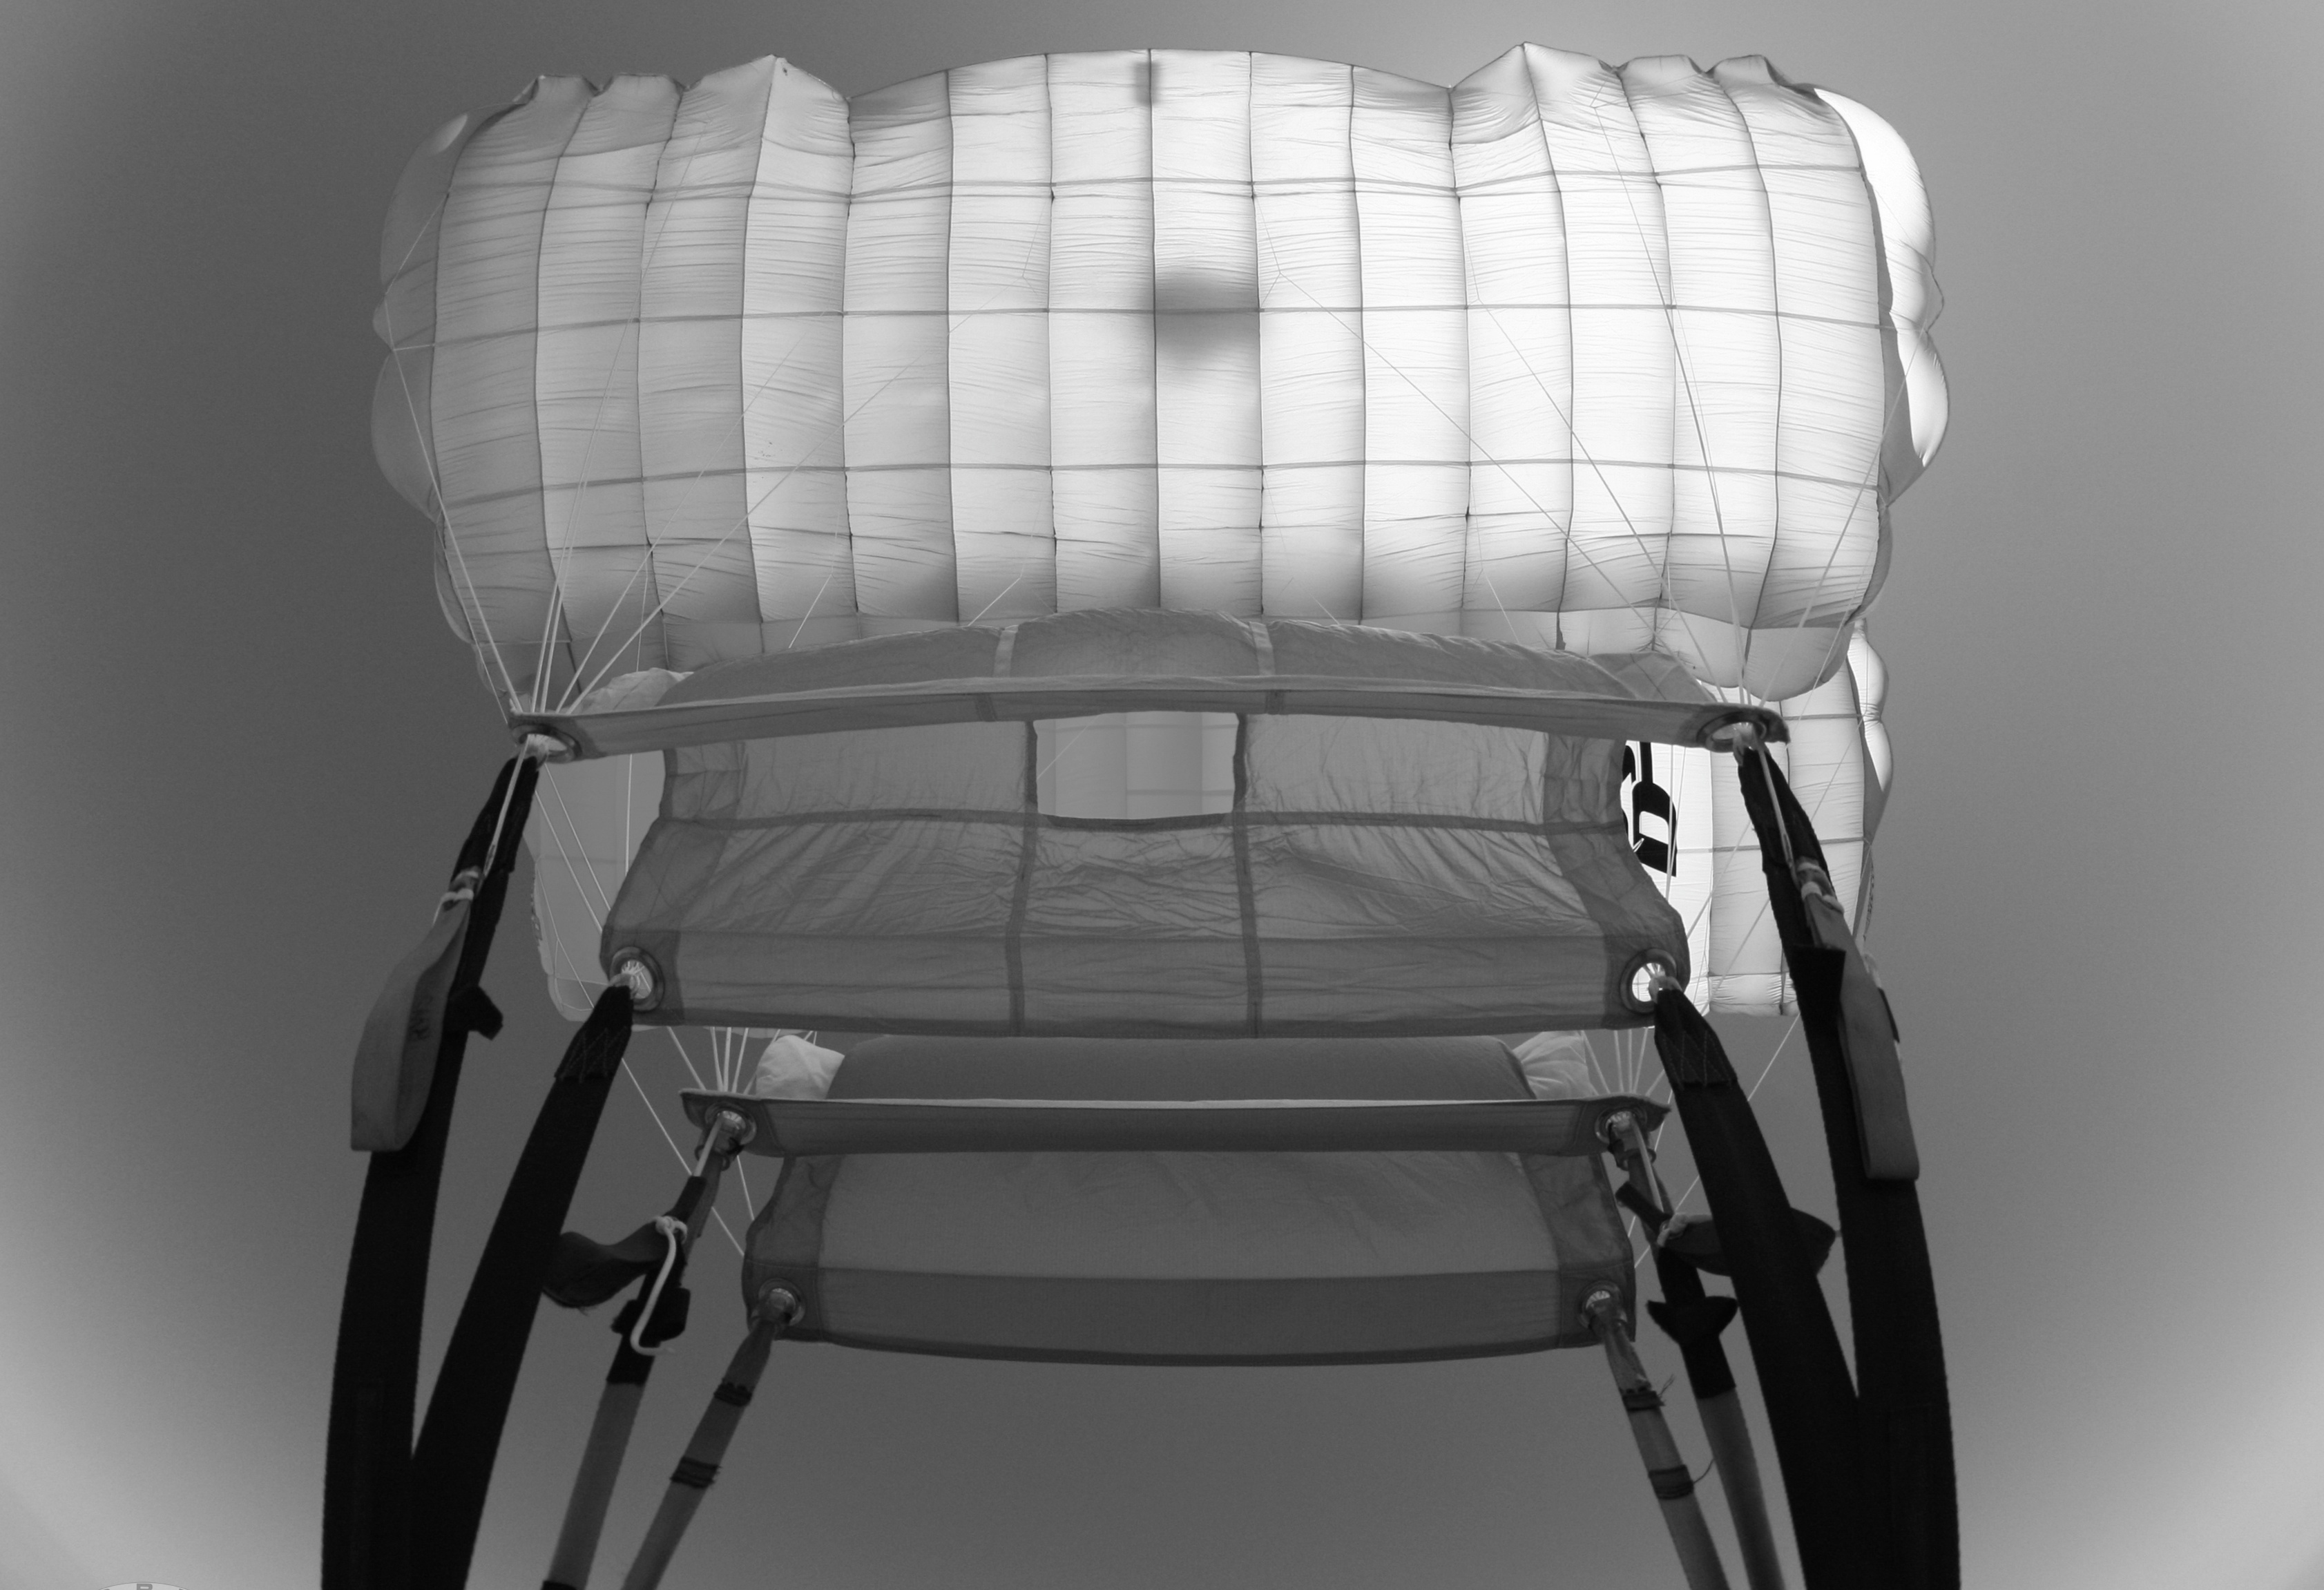
\includegraphics[width=0.95\textwidth]{2-kupua-biplane.jpeg}\captionof{figure}{Varjot peräkkäin (biplane)}\end{Figure} 

\subsubsection{ Varjot vierekkäin (side-by-side) }
\label{mahdolliset-vaaratilanteet-varjot-vierekkain-side-by-side}


Ohjaa varovasti hallitsevaa varjoa vain välttämättömillä ohjausliikkeillä takimmaisista kantohihnoista. Älä avaa puolijarruja. Älä jarruta alastulossa ja valmistaudu kovaan alastuloon. 


\textbf{Älä päästä päävarjoa irti!}  


\begin{Figure}\centering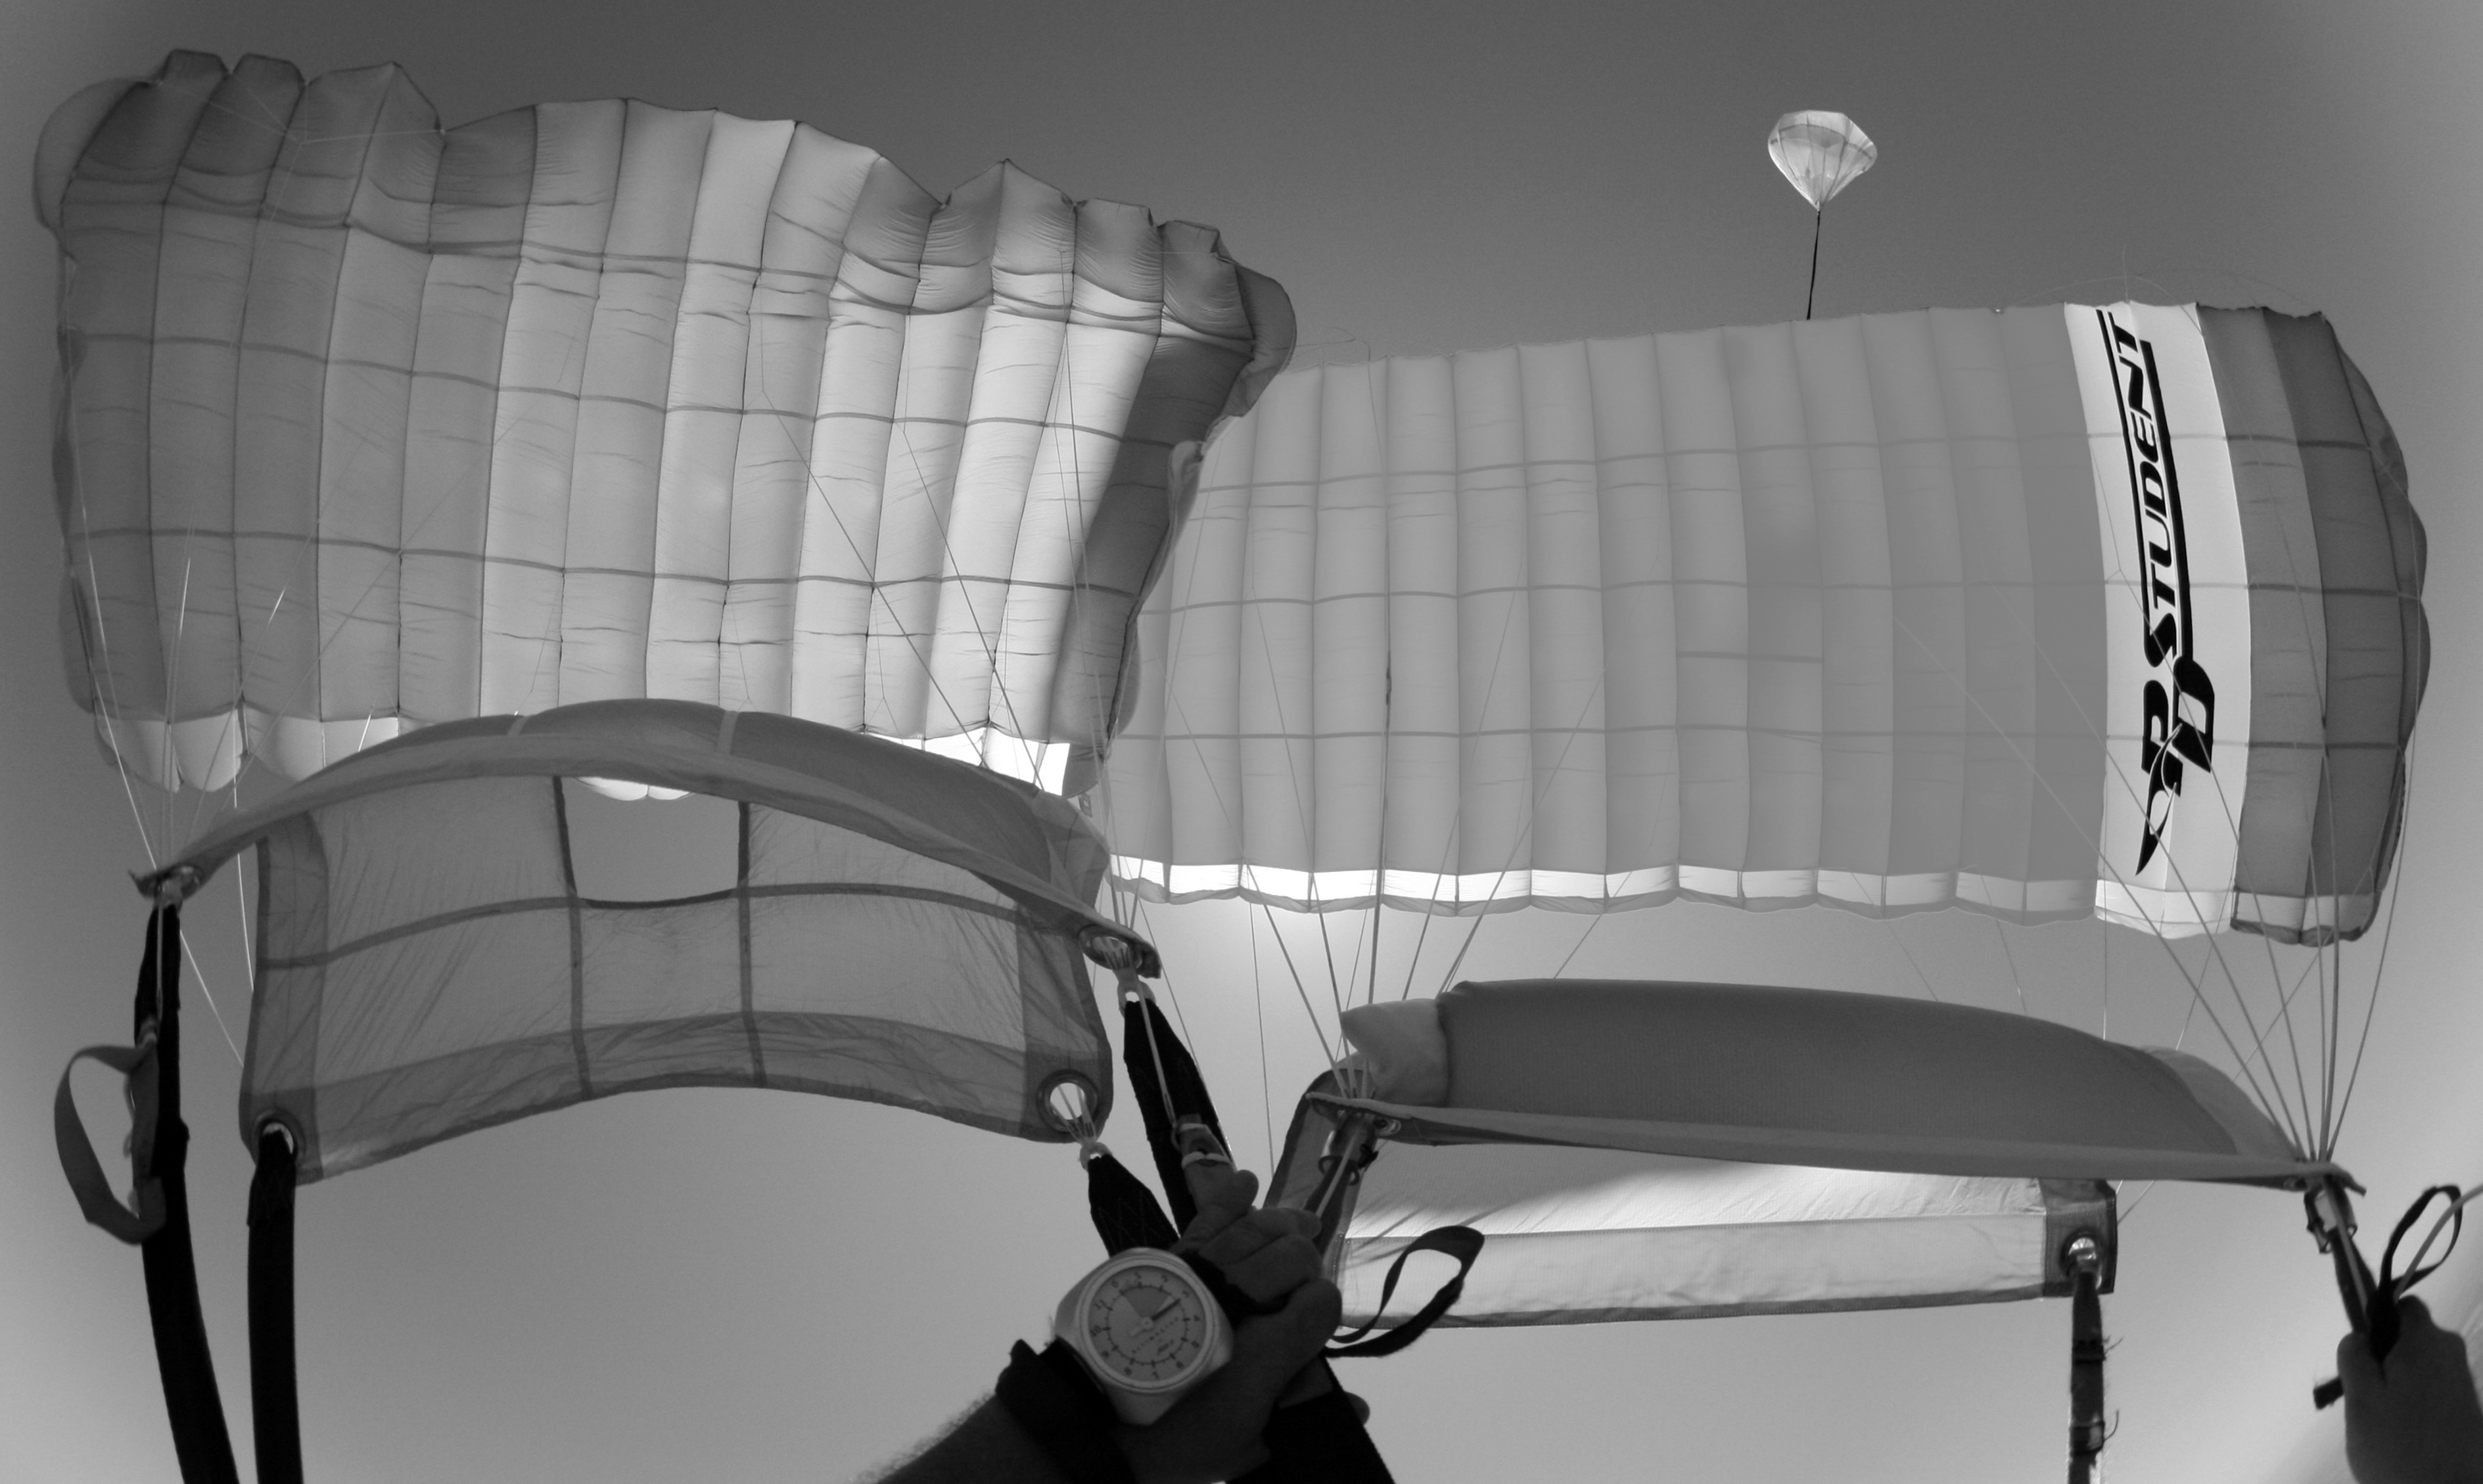
\includegraphics[width=0.95\textwidth]{2-kupua-sidebyside.jpeg}\captionof{figure}{Varjot vierekkäin (side-by-side)}\end{Figure} 

\subsubsection{ Varjot sivuilla, vajoavat nopeasti (downplane) }
\label{mahdolliset-vaaratilanteet-varjot-sivuilla-vajoavat-nopeasti-downplane}


Tämä lentotila on harvinainen. Varjot voivat siirtyä itsestään varjot vierekkäin -muodostelmaan. 


\textbf{Päästä päävarjo irti!} 


\begin{Figure}\centering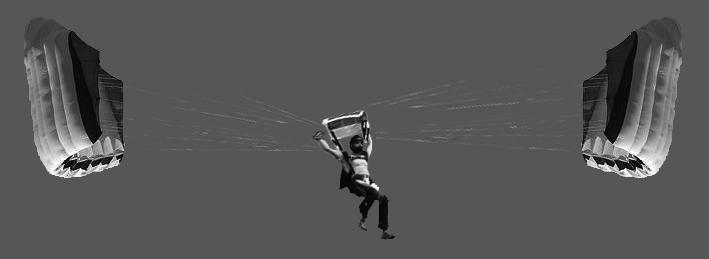
\includegraphics[width=0.95\textwidth]{2-kupua-downplane.jpeg}\captionof{figure}{Varjot sivuilla (downplane)}\end{Figure} 

\subsection{ Törmääminen varjon varassa }
\label{mahdolliset-vaaratilanteet-tormaaminen-varjon-varassa}


Törmäys on mahdollinen aina, kun ilmassa on useita hyppääjiä. Heti, kun olet tarkastanut, että varjo lentää, tarkasta ilmatila ja ole valmiina väistämään. Ennen puolijarrujen avaamista voit ohjata varjoa takimmaisista kantohihnoista (mikäli punokset eivät ole kierteellä). Väistä \textbf{oikealle!} 


Katso aina ennen käännöstä käännöksen suuntaan varmistaaksesi vapaa ilmatila. Alempana olevalla on aina etuajo-oikeus. Jos et voi välttää törmäämistä, minimoi törmäysvauhti jarruttamalla voimakkaasti sekä käperry \textit{palloksi.} Varoita toista hyppääjää huutamalla. 


Sotkeutumistilanteessa: 

\begin{itemize}
\item  Tarkkaile korkeutta, sillä päätökset on tehtävä riittävän korkealla 
\item  Keskustele aina kaverisi kanssa siitä, mitä aiotte tehdä 
\item  Varmista, että olet irti punoksista/kuvusta (käytä tarvittaessa koukkupuukkoa) ennen varavarjotoimenpiteitä. 
\end{itemize}

Jos ylempi varjo lentää ja alempi on sotkeutunut, voi alempi hyppääjä tehdä varavarjotoimenpiteet ja ylempi yleensä laskeutua päävarjollaan. Jos varjot ovat sotkeutuneet toisiinsa, joutuvat luultavasti molemmat tekemään varavarjotoimenpiteet. Tällöin molempien pitää sopia, missä järjestyksessä toimitaan, jotta vältetään törmääminen varavarjojen varassa. Jos korkeutta on liian vähän varavarjotoimenpiteisiin (alle 300 m), voi kaksikin ihmistä laskeutua yhdellä varjolla. 


Huomioi kaikissa toimenpiteissäsi ajan ja korkeuden menetys. 

\section{ Laskeutuminen epätavallisiin paikkoihin  }
\label{mahdolliset-vaaratilanteet-laskeutuminen-epatavallisiin-paikkoihin}


Laskeutumisen muihin paikkoihin kuin maalialueelle voi yleensä välttää ohjaamalla oikein. Alussa korkeuden ja kuljettavan matkan arviointi voi olla hankalaa, mutta hyppykokemuksen karttuessa tämäkin taito kehittyy. Joskus uloshyppypaikka voi olla väärä. Näin voi käydä etenkin, jos tuulet ovat yllättäen muuttuneet. Oli syy väärään uloshyppypaikkaan mikä tahansa, ajoissa tehty varalaskusuunnitelma mahdollistaa turvallisen laskeutumisen myös maalialueen ulkopuolelle. Suunnitelman muuttaminen viime hetkellä on vaarallista! 


Hyviä varalaskupaikkoja ovat esimerkiksi pellot ja muut aukeat alueet. Riippumatta siitä, mihin laskeudut, pyri aina laskeutumaan vastatuuleen! Pääasia on kuitenkin, että et tee jyrkkiä käännöksiä matalalla. Muista aina ottaa hyvä alastuloasento ja pitää se tiukasti maahan asti. 


Maalialueen ulkopuolelle laskeutuessasi et välttämättä enää loppuvaiheessa näe tuulipussia. Paina siksi mieleesi jo hypylle lähtiessäsi esimerkiksi se, missä suunnassa aurinko on, kun olet kääntynyt vastatuuleen. Liput, viirit ja savut ovat myös hyviä tuulen suunnan osoittimia. 

\subsection{ Laskeutuminen veteen }
\label{mahdolliset-vaaratilanteet-laskeutuminen-veteen}


Laskeudu mieluummin metsään kuin veteen. Joutuessasi laskeutumaan veteen pyri niin lähelle rantaa kuin mahdollista. Veteen laskeutuessasi toimi seuraavasti: 

\begin{itemize}
\item  Vapauta varavarjon pakkolaukaisuhihna 
\item  Käännä FXC OFF-asentoon 
\item  Löysää rintahihna 
\item  Ota alastuloasento 
\item  Tee loppuveto ennen veteen tuloa. 
\end{itemize}

Vedessä: 

\begin{itemize}
\item  Tukahduta varjo tarvittaessa tekemällä päävarjon irtipäästö 
\item  Avaa hihnat ja ui eroon varjosta. 
\end{itemize}
\subsection{ Laskeutuminen puuhun/metsään }
\label{mahdolliset-vaaratilanteet-laskeutuminen-puuhun-metsaan}


Puuhun tai metsään laskeutuessasi toimi seuraavasti: 

\begin{itemize}
\item  Vältä yksittäisiä ja korkeita puita 
\item  Ota alastuloasento ja vedä polvet ylös suojaamaan alavartaloa 
\item  Tee loppuveto puiden latvoihin sekä pidä kyynärpäät kyljissä kiinni 
\item  Valmistaudu tulemaan maahan asti ja pura alastuloasento vasta, kun liike loppuu. 
\end{itemize}

Jos jäät puuhun roikkumaan, älä pudottaudu korkealta, vaan odota apua. 


Suuri vaakanopeus aiheuttaa enemmän kolhuja kuin suuri vajoamisnopeus. Loppuvedon tekeminen puiden latvoihin on turvallisempaa kuin puita päin lentäminen. 

\subsection{ Laskeutuminen sähkölinjoihin }
\label{mahdolliset-vaaratilanteet-laskeutuminen-sahkolinjoihin}


Jos joudut laskeutumaan sähkölinjoihin, niin 

\begin{itemize}
\item  Heitä mahdollisesti käsissäsi olevat kahvat pois 
\item  Ohjaa varjoa loppuun saakka 
\item  Ota alastuloasento ja tee loppuveto linjoihin 
\item  Estä johtimien meno jalkojen väliin tai kainaloihin 
\item  Jos varjo jää kiinni, \textbf{älä yritä irrottaa sitä} 
\item  Odota apua. 
\end{itemize}
\subsection{ Laskeutuminen katolle }
\label{mahdolliset-vaaratilanteet-laskeutuminen-katolle}


Mikäli joudut laskeutumaan katolle, toimi seuraavasti: 

\begin{itemize}
\item  Ota alastuloasento 
\item  Tee loppuveto katolle 
\item  Tukahduta varjo välittömästi ja tee tarvittaessa päävarjon irtipäästö 
\item  Tartu kiinni kattorakenteista 
\item  Odota apua. 
\end{itemize}
\subsection{ Kiinteään esteeseen törmääminen }
\label{mahdolliset-vaaratilanteet-kiinteaan-esteeseen-tormaaminen}


Näitä ovat esimerkiksi seinät, autot, pylväät ja aidat. Jos osut kiinteään esteeseen, 

\begin{itemize}
\item  Tee loppuveto ennen törmäystä 
\item  Ota isku vastaan jaloilla 
\item  Valmistaudu maahantuloon 
\end{itemize}

Hyvän alastuloasennon merkitys korostuu, jos joudut laskeutumaan muualle kuin maalialueelle. 

\end{multicols}

\chapter{NOVA-Alkeiskoulutuksen suoritukset}
\label{nova-alkeiskoulutuksen-suoritukset}
\thispagestyle{headings}
\begin{multicols}{2}

NOVA-koulutusohjelmassa oppilaalle annetaan henkilökohtaista koulutusta. Tasokoulutus koostuu seitsemästä erilaisesta tasosta. Jokaisella tasohypyllä on mukana vähintään yksi novahyppymestari. Tasokoulutuksessa edetään omaa tahtia. Jokaisella hypyllä hyödynnetään edellisten tasojen osaamista, joten oppilaan on suoritettava kukin taso hyväksytysti ennen etenemistä. 


Oppilaan on saavutettava välttämättömät oppimistavoitteet hyväksytysti päästäkseen seuraavalle tasolle. Jos ensimmäisen hypyn koulutuksesta on kulunut jonkin aikaa eikä sitä jostain syystä ole hypätty, koulutus on annettava uudelleen.  

\section{ Vapaapudotus NOVA-hypyillä }
\label{nova-alkeiskoulutuksen-suoritukset-vapaapudotus-nova-hypyilla}


Ulos hypätessä taivuta lantiosta, siirrä kädet ja jalat oikeaan asentoon ja pidä katse koneessa niin kauan kuin mahdollista. Pyri rentoutumaan puhaltamalla ulos hengittäessä suun kautta ja pidä leuka ylhäällä. Kuvittele puskevasi lantiota ilman halki. 

\subsection{Tarkkailukehä}
\label{nova-alkeiskoulutuksen-suoritukset-tarkkailukeha}


Laskettuasi 105:een aloita ja suorita omatoimisesti tarkkailukehä: 

\begin{enumerate}[label=\bfseries \arabic*)]
\item  MAA 
	\begin{itemize}
	\item  Siirrä katseesi 45° kulmassa alaspäin ja valitse jokin iso ja helposti löydettävä kiintopiste 
	\end{itemize}
\item  MITTARI 
	\begin{itemize}
	\item  Pidä taivutus, siirrä katseesi mittariin ja lue lukema. 
	\end{itemize}
\item  KORKEUS (VV-HM, varavarjon puoleinen hyppymestari) 
	\begin{itemize}
	\item  Katso vasemmalla puolella olevaa hyppymestaria käsivarren alta ja sano hänelle korkeusmittarin lukema. Hyppymestari voi tässä vaiheessa korjata asentoasi käsimerkein. Jos asennossa ei ole mitään korjattavaa, saat OK-käsimerkin (peukalo ylös). Älä jatka tarkkailukehää ennen kuin olet saanut OK-käsimerkin! 
	\end{itemize}
\item  KORKEUS (PV-HM, päävarjon puoleinen hyppymestari) 
	\begin{itemize}
	\item  Katso oikealla puolella olevaa hyppymestaria käsivarren alta ja suorita sama toimenpide kuin edellä. Jos kaikki on kunnossa saat OK-käsimerkin. Älä jatka tarkkailukehää ennen kuin olet saanut OK-käsimerkin! 
	\end{itemize}
\end{enumerate}

Tarkkailukehän avulla säilytät tietoisuuden korkeudesta ja suunnasta.  

\subsection{Harjoitusveto}
\label{nova-alkeiskoulutuksen-suoritukset-harjoitusveto}


Aloita itsenäisesti, mutta jos näet harjoitusveto-käsimerkin, se merkitsee harjoitusvedon aloittamista. Toimi rytmikkäästi ja sano toimenpiteet ääneen. 

\begin{enumerate}[label=\bfseries \arabic*)]
\item  TAIVUTA 
	\begin{itemize}
	\item  Työnnä lantiota alaspäin / varmista taivutus. 
	\item  Taivutus säilyy ja leuka pysyy ylhäällä koko harjoitusvedon ajan. 
	\end{itemize}
\item  TARTU 
	\begin{itemize}
	\item  Pidä katse ylhäällä. Siirrä vasen käsi pääsi yläpuolelle siten, että peukalo koskettaa päätäsi (otsaa) kämmenen ollessa auki. Siirrä oikea kätesi päävarjon avauskahvalle kämmen auki. Käsien liikkeiden on tapahduttava symmetrisesti, samalla tasolla ja yhdenaikaisesti. Vain kädet liikkuvat. Pään tai muun vartalon asento ei muutu.  
	\item  Kosketa kahvaa ja paina mieleesi kahvan paikka. On tärkeää tuntea selvästi, missä se on.   
	\end{itemize}
\item  VEDÄ 
	\begin{itemize}
	\item  Palauta kädet alkuperäiseen asentoon symmetrisesti ja yhdenaikaisesti. Vain kädet liikkuvat. Pään tai muun vartalon asento ei muutu. Huom! Kyseessä on harjoitusveto, joten älä vedä oikeasti. 
	\end{itemize}
\end{enumerate}
\subsection{ Varjon avaus }
\label{nova-alkeiskoulutuksen-suoritukset-varjon-avaus}


Ensimmäisellä hypylläsi aloitat avaustoimenpiteet 1600 metrin korkeudessa. Näytä ensin avausmerkki, jolla ilmoitat muille avaavasi varjosi, eli heilauta käsiäsi ristiin pääsi edessä. Avausmerkin jälkeen aloitat rauhallisesti ja täsmällisesti avaustoimenpiteet. Avaus tehdään samalla tavalla kuin harjoitusveto. Erona on vain se, että apuvarjon kahvasta tartutaan kunnolla kiinni ja apuvarjo heitetään reippaasti ilmavirtaan. Varjon ei siis pidä olla auki heti 1600 metrissä.  


TAIVUTA - TARTU - VEDÄ 


Tämän jälkeen laske ääneen 101, 102…105, jonka jälkeen tarkistat varjon ja suoritat mahdolliset selvitystoimenpiteet. Mikäli varjo ei selviä tai ei lennä, tee varavarjotoimenpiteet. Tasoilla 1-2 VV-HM pitää sinusta kiinni varjon avautumiseen asti ja tasoilla 3-7 HM varmistaa avautumisen.  

\section{ Taso 1 - Tottuminen vapaapudotukseen }
\label{nova-alkeiskoulutuksen-suoritukset-taso-1-tottuminen-vapaapudotukseen}


Kaksi novahyppymestaria, kolmella ensimmäisellä hypyllä radio. 


Jos näet vain yhden hyppymestarin, seuraa hänen ohjeitaan ja jatka hyppysuoritusta normaalisti ohjelman mukaan. Tasoilla 1 ja 2 \textbf{et} saa olla yksin vapaapudotuksessa. Jos et näe kumpaakaan hyppymestaria, avaa varjo välittömästi eli TAIVUTA-TARTU-VEDÄ 101..105 ja tarkista varjo.  

\subsection{ Oppilaan toiminta. }
\label{nova-alkeiskoulutuksen-suoritukset-oppilaan-toiminta}


Harjoittele 1. tason kulku (ja myöhemmin kaikki muut tasot) mahdollisimman hyvin etukäteen, sillä se helpottaa ja nopeuttaa huomattavasti oppimistasi. 

\subsection{ Ensimmäiseen hyppyysi valmistautuminen }
\label{nova-alkeiskoulutuksen-suoritukset-ensimmaiseen-hyppyysi-valmistautuminen}

\begin{enumerate}[label=\bfseries \arabic*)]
\item  Näytä, miten koneen ovelle siirrytään hyppyasentoon. 
\item  Esitä oikea hallittu uloshyppy mukaan lukien laskeminen. 
\item  Käy läpi ja harjoittele suunniteltu hyppy kohta kohdalta. 
\item  Harjoittele harjoitusvetoa samalla tavalla kuin oikeaa avausliikettä. 
	\begin{itemize}
	\item  a. TAIVUTA taivutus säilyy. Katse eteenpäin leuka ylhäällä. 
	\item  b. TARTU säilytä taivutus, kun siirrät samanaikaisesti oikean käden kämmen auki päävarjon avauskahvalle ja siirrä vasen käsi pääsi yläpuolelle siten, että peukalo koskettaa päätäsi (otsaa) kämmen avattuna. Paina tarkasti mieleesi kahvan paikka. Molemmat kädet pysyvät samassa tasossa. Vain kädet liikkuvat, ei pää eikä muu vartalon osa. Katse eteenpäin leuka ylhäällä. 
	\item  c. VEDÄ palauta kädet alkuperäiseen asentoon symmetrisesti sekä yhdenaikaisesti, katse eteenpäin ja leuka ylhäällä. Vain kädet liikkuvat, pään tai muun vartalon asento ei muutu lainkaan. HUOM. Tämä on harjoitusveto, joten älä vedä oikeasti.  
	\end{itemize}
\item  Harjoittele toimenpiteitä lennon ja hypyn aikana sattuvien vaaratilanteiden varalta. 
\item  Katso maatuulen suunta tuulipussista ja kuvaile oikeat ohjauskuviot. 
\item  Näytä oikea alastulo- ja kaatumisasento. 
\item  Kertaa käsimerkit. 
\end{enumerate}
\subsection{ Oppimistavoitteet }
\label{nova-alkeiskoulutuksen-suoritukset-oppimistavoitteet}


Jokaisella tasolla on omat oppimistavoitteet, joiden mukaan arvioidaan oppimisesi, sekä se, pääsetkö seuraavalle tasolle. Tutustu oppimistavoitteisiin tarkasti HM:n kanssa. 

\begin{enumerate}[label=\bfseries \arabic*)]
\item  Stabiilin vapaapudotusasennon löytäminen viimeistään 10 sekuntia ennen avauskorkeutta 
\item  Korkeuden tarkkailu 
\item  Avausmerkki 1600 m (±300m) ja avaus 
\end{enumerate}
\subsection{ Hyppylennolla }
\label{nova-alkeiskoulutuksen-suoritukset-hyppylennolla}

\begin{itemize}
\item  Katso laskeutumisalue ja oikea laskeutumissuunta yli 600 m:n korkeudessa. Hyppymestari kysyy tärkeitä korkeuksia. 
\item  Hyppymestari kysyy hypyn avainkohdat. 
\end{itemize}
\subsection{ Hypyn kulku }
\label{nova-alkeiskoulutuksen-suoritukset-hypyn-kulku}

\begin{tabular}[]{|l|p{4.7cm}|}
\hline
 \textbf{2700-4000 m} &  Rento taivutettu UH
\\ \hline
  &  Tarkkailukehä
\\ \hline
  &  3 Harjoitusvetoa
\\ \hline
  &  Tarkkailukehä
\\ \hline
  &  MAA - MITTARI
\\ \hline
 \textbf{1600 m} &  Avausmerkki ja avaus
\\ \hline
\end{tabular}

\end{multicols}\pagebreak\begin{multicols}{2} 

\section{ Taso 2 - Asennon hallinta }
\label{nova-alkeiskoulutuksen-suoritukset-taso-2-asennon-hallinta}


Kaksi novahyppymestaria, kolmella ensimmäisellä hypyllä radio.   Oppilaan on saavutettava välttämättömät oppimistavoitteet hyväksytysti päästäkseen seuraavalle tasolle. 

\subsection{ Oppilaan toiminta. }
\label{nova-alkeiskoulutuksen-suoritukset-oppilaan-toiminta}

\begin{enumerate}[label=\bfseries \arabic*)]
\item  Käy läpi I-tasolla opitut tiedot ja taidot. 
\item  Harjoittele stabiilia asentoa esim. rullalaudoilla. 
\item  Harjoittele kaikkia vapaassa tehtäviä liikkeitä kuten aikaisemmilla tunneilla. 
\item  Harjoittele harjoitusvetoa kuten oikeaa avausta. 
\item  Näytä maalialue ja käy läpi ennalta suunniteltu ohjauskuvio. 
\item  Käytä mielikuvaharjoittelua valmistautuessasi hyppyyn. 
\item  Osallistu itse aikaisempaa enemmän varusteiden tarkistukseen ja sovittamiseen. 
\end{enumerate}
\subsection{ Oppimistavoitteet }
\label{nova-alkeiskoulutuksen-suoritukset-oppimistavoitteet}

\begin{enumerate}[label=\bfseries \arabic*)]
\item  Stabiili vapaapudotusasento viimeistään 10 sekuntia UH:n jälkeen 
\item  Stabiilin vapaapudotusasennon säilyttäminen koko hypyn ajan, sisältäen jalkojen hallinnan 
\item  Avausmerkki 1600 m (±150 m) ja itsenäinen avaus  
\item  Itsenäisempi, turvallinen varjon ohjailu 
\end{enumerate}
\subsection{ Hyppylennolla }
\label{nova-alkeiskoulutuksen-suoritukset-hyppylennolla}

\begin{enumerate}[label=\bfseries \arabic*)]
\item  Toista kaikki aikaisemmin opetetut toimenpiteet lennon aikana. 
\item  Käytä rentouttavaa hengitystekniikkaa (hengitä hitaasti sisään, pidätä hetkisen ja rentoudu uloshengittäessäsi). 
\item  Näytä maamerkkejä ja osoita avauskorkeus hyppymestareille. 
\end{enumerate}
\subsection{ Hypyn kulku }
\label{nova-alkeiskoulutuksen-suoritukset-hypyn-kulku}

\begin{tabular}[]{|l|p{4.7cm}|}
\hline
 \textbf{2700-4000 m} &  Rento, taivutettu uloshyppy
\\ \hline
  &  Tarkkailukehä
\\ \hline
  &  Harjoitusvetoja kunnes OK
\\ \hline
  &  MAA, MITTARI, TAIVUTA, JALAT, RENTOUTA
\\ \hline
  &  Liike eteenpäin
\\ \hline
  &  MAA, MITTARI, TAIVUTA, JALAT, RENTOUTA
\\ \hline
  &  90° vasen
\\ \hline
  &  MAA, MITTARI, TAIVUTA, JALAT, RENTOUTA
\\ \hline
  &  90° oikea
\\ \hline
  &  MAA, MITTARI, TAIVUTA, JALAT, RENTOUTA
\\ \hline
 \textbf{1600 m} &  Avausmerkki ja avaus
\\ \hline
\end{tabular}

\end{multicols}\pagebreak\begin{multicols}{2} 

\section{ Taso 3 - Stabiili vapaapudotus }
\label{nova-alkeiskoulutuksen-suoritukset-taso-3-stabiili-vapaapudotus}


Kaksi novahyppymestaria, kolmella ensimmäisellä hypyllä radio. 


Oppilaan on saavutettava välttämättömät oppimistavoitteet hyväksytysti päästäkseen seuraavalle tasolle. 


Jos tasoilla 3-7 et näe kumpaakaan hyppymestaria, voit jatkaa hyppyä, mikäli kaikki alla olevat ehdot täyttyvät: 

\begin{itemize}
\item  Tiedät korkeutesi  
\item  Et pyöri mihinkään suuntaan 
\item  Et ole selälläsi 
\item  Tilanne tuntuu kaiken kaikkiaan olevan hallinnassa 
\end{itemize}

Tarkkaile korkeutta koko ajan n. 5 s välein (MAA, MITTARI, TAIVUTA, JALAT, RENTOUTA) ja tason mukaisessa korkeudessa tee avausmerkki ja avaa päävarjo normaalisti. Älä tee muita suorituksia.  


Jos et avauksessa löydä päävarjon kahvaa, yritä toisen kerran, mutta jos et \textbf{heti} löydä kahvaa, tee varavarjotoimenpiteet. 


Jos et avauksessa jaksa vetää päävarjon kahvasta (tiukka kahva), yritä toisen kerran, mutta jos et silloinkaan \textbf{heti} saa varjoa auki, tee varavarjotoimenpiteet. 

\subsection{ Oppilaan toiminta. }
\label{nova-alkeiskoulutuksen-suoritukset-oppilaan-toiminta}

\begin{enumerate}[label=\bfseries \arabic*)]
\item  Kuvaile ja esitä käytännössä tiedot ja taidot, jotka on opittu aikaisempien hyppyjen yhteydessä. 
\item  Harjoitteleilmatilan tarkistusta HM:n avustuksella. 
\item  Harjoittele maassa tekniikkaa jolla käännyt tarvittaessa selältään oikein päin. 
\item  Näytä millä tekniikalla suunta säilytetään vapaapudotuksessa. 
\item  Keskity hyppyyn ja rentoudu. Mieti, millainen on hyvä stabiili asento ja harjoittele sitä. 
\item  Käy läpi hypyn kulku ja harjoittele sitä käytännössä. 
\end{enumerate}
\subsection{ Oppimistavoitteet }
\label{nova-alkeiskoulutuksen-suoritukset-oppimistavoitteet}

\begin{enumerate}[label=\bfseries \arabic*)]
\item  Ilmatilan tarkistus ennen uloshyppyä 
\item  Stabiili itsenäinen vapaapudotus viimeistään 5 sekuntia UH:n jälkeen 
\item  Tarkoituksettomien käännösten pysäyttäminen 
\item  Avausmerkki 1600 m (±150m), stabiili itsenäinen avustamaton avaus ilman NHM:n otetta oppilaasta 
\item  Itsenäinen, turvallinen varjon ohjailu 
\end{enumerate}
\subsection{ Hyppylennolla }
\label{nova-alkeiskoulutuksen-suoritukset-hyppylennolla}

\begin{enumerate}[label=\bfseries \arabic*)]
\item  Toista aiemmin opitut toimenpiteet. 
\item  Käytä rentouttavaa hengitystekniikkaa ja positiivisia mielikuvia. 
\item  Katso HM:n johdolla lentokenttää ja ilmatilaa ovella ennen uloshyppyä. 
\end{enumerate}
\subsection{ Ohjailu ja laskeutuminen }
\label{nova-alkeiskoulutuksen-suoritukset-ohjailu-ja-laskeutuminen}

\begin{enumerate}[label=\bfseries \arabic*)]
\item  Toimi kuten edellisillä hypyillä, mutta tee kaikki entistä tarkemmin. 
\item  Seisontalaskua saa yrittää (mutta pidä aina hyvä alastuloasento). 
\end{enumerate}
\subsection{ Hypyn kulku }
\label{nova-alkeiskoulutuksen-suoritukset-hypyn-kulku}

\begin{tabular}[]{|l|p{4.7cm}|}
\hline
 \textbf{2700-4000 m} &  Rento taivutettu UH
\\ \hline
  &  Tarkkailukehä
\\ \hline
  &  Harjoitusvetoja kunnes OK
\\ \hline
  &  Stabiili itsenäinen vapaapudotus
\\ \hline
  &  MAA, MITTARI, TAIVUTA, JALAT, RENTOUTA
\\ \hline
 \textbf{1600 m} &  Avausmerkki ja avaus
\\ \hline
\end{tabular}

\end{multicols}\pagebreak\begin{multicols}{2} 

\section{ Taso 4 - Käännökset 90° }
\label{nova-alkeiskoulutuksen-suoritukset-taso-4-kaannokset-90deg}


Yksi novahyppymestari. 


Oppilaan on saavutettava välttämättömät oppimistavoitteet hyväksytysti päästäkseen seuraavalle tasolle. 

\subsection{ Oppilaan toiminta. }
\label{nova-alkeiskoulutuksen-suoritukset-oppilaan-toiminta}

\begin{enumerate}[label=\bfseries \arabic*)]
\item  Osaat tehdä varusteiden tarkastuksen maassa ja ennen koneelle menoa. (\ref{laskuvarjokalusto-ja-hyppyvarusteet-3x3-tarkastus} s.\pageref{laskuvarjokalusto-ja-hyppyvarusteet-3x3-tarkastus}) 
\item  Harjoittele koko hyppytapahtuman kulku käytännössä. 
\item  Tarkista ilmatila ja pilvet ennen uloshyppyä ja huomioi riittävä exit-väli edelliseen ryhmään. 
\item  Tarkista varusteet ennen UH:ta (\ref{laskuvarjokalusto-ja-hyppyvarusteet-3x3-tarkastus} s.\pageref{laskuvarjokalusto-ja-hyppyvarusteet-3x3-tarkastus}) 
\end{enumerate}
\subsection{ Oppimistavoitteet }
\label{nova-alkeiskoulutuksen-suoritukset-oppimistavoitteet}

\begin{enumerate}[label=\bfseries \arabic*)]
\item  Ilmatilan ja pilvien tarkistus ja exit-väli  
\item  Omien varusteiden tarkastus (maassa ja koneessa) 
\item  Stabiili vapaapudotusasento 
\item  Vähintään kaksi hallittua 90° käännöstä (±20°) 
\item  Avausmerkki 1500 m (±150 m), stabiili itsenäinen avustamaton avaus  
\end{enumerate}
\subsection{ Hyppylennolla }
\label{nova-alkeiskoulutuksen-suoritukset-hyppylennolla}

\begin{enumerate}[label=\bfseries \arabic*)]
\item  Toimi lennon aikana aikaisemmin opetettujen toimenpiteiden mukaisesti. 
\item  Tarkista ilmatila ja pilvet sekä huomioi riittävä exit-väli edelliseen ryhmään. 
\end{enumerate}
\subsection{ Ohjailu ja laskeutuminen }
\label{nova-alkeiskoulutuksen-suoritukset-ohjailu-ja-laskeutuminen}

\begin{enumerate}[label=\bfseries \arabic*)]
\item  Toimi aiemmin opitulla tavalla. 
\item  Pyri laskeutumaan korkeintaan 50 m päähän kohteesta mahdollisimman vähin ohjein. 
\end{enumerate}
\subsection{ Hypyn kulku }
\label{nova-alkeiskoulutuksen-suoritukset-hypyn-kulku}

\begin{tabular}[]{|l|p{4.7cm}|}
\hline
 \textbf{2700-4000 m} &  Rento taivutettu UH
\\ \hline
  &  Tarkkailukehä (HM siirtyy oppilaan eteen)
\\ \hline
  &  Lupa käännökseen (oppilas nyökkää HM:lle, HM vastaa nyökkäämällä)
\\ \hline
  &  90° vasen
\\ \hline
  &  MAA, MITTARI, TAIVUTA, JALAT, RENTOUTA
\\ \hline
  &  90° oikea
\\ \hline
  &  MAA, MITTARI, TAIVUTA, JALAT, RENTOUTA
\\ \hline
 \textbf{2000 m} &  Ei käännöksiä
\\ \hline
  &  MAA, MITTARI, TAIVUTA, JALAT, RENTOUTA
\\ \hline
 \textbf{1500 m} &  Avausmerkki ja avaus
\\ \hline
\end{tabular}

\end{multicols}\pagebreak\begin{multicols}{2} 

\section{ Taso 5 - Käännökset 360° }
\label{nova-alkeiskoulutuksen-suoritukset-taso-5-kaannokset-360deg}


Yksi novahyppymestari. 


Oppilaan on saavutettava välttämättömät oppimistavoitteet hyväksytysti päästäkseen seuraavalle tasolle. 

\subsection{ Oppilaan toiminta. }
\label{nova-alkeiskoulutuksen-suoritukset-oppilaan-toiminta}

\begin{enumerate}[label=\bfseries \arabic*)]
\item  Näytä, että osaat oikeaoppisesti tarkastaa ja säätää varusteet. 
\item  Harjoittele koko hyppytapahtuman kulku käytännössä. 
\item  Tarkistat ilmatilan, pilvet ja huomioit exit-välin  
\item  Tarkastat automaattisesti itse varusteet ennen uloshyppyä. (\ref{laskuvarjokalusto-ja-hyppyvarusteet-3x3-tarkastus} s.\pageref{laskuvarjokalusto-ja-hyppyvarusteet-3x3-tarkastus}) 
\end{enumerate}
\subsection{ Oppimistavoitteet }
\label{nova-alkeiskoulutuksen-suoritukset-oppimistavoitteet}

\begin{enumerate}[label=\bfseries \arabic*)]
\item  Vähintään kaksi hallittua 360° käännöstä (±45°) 
\item  Yhä stabiilimpi vapaapudotus  
\item  Avausmerkki 1500 m (±150 m), stabiili suunnassa pysyvä itsenäinen avustamaton avaus   
\item  Tee varjon varassa 90° käännöksiä takimmaisista kantohihnoista puolijarrut kiinni sekä avattuina 
\end{enumerate}
\subsection{ Hyppylennolla }
\label{nova-alkeiskoulutuksen-suoritukset-hyppylennolla}

\begin{enumerate}[label=\bfseries \arabic*)]
\item  Tarkistat ilmatilan, pilvet ja huomioit exit-välin. 
\item  Tarkastat itse varusteet ennen uloshyppyä 
\end{enumerate}
\subsection{ Ohjailu ja laskeutuminen }
\label{nova-alkeiskoulutuksen-suoritukset-ohjailu-ja-laskeutuminen}

\begin{enumerate}[label=\bfseries \arabic*)]
\item  Tee 90° käännöksiä kantohihnoista puolijarrut kiinni sekä avattuina. 
\item  Pyri laskeutumaan enintään 50 metrin päähän kohteesta. 
\item  Muista oikea lähestymis- ja laskeutumistekniikka. 
\end{enumerate}
\subsection{ Hypyn kulku }
\label{nova-alkeiskoulutuksen-suoritukset-hypyn-kulku}

\begin{tabular}[]{|l|p{4.7cm}|}
\hline
 \textbf{2700-4000 m} &  Rento taivutettu UH
\\ \hline
  &  Tarkkailukehä (HM siirtyy oppilaan eteen)
\\ \hline
  &  Lupa käännökseen (oppilas nyökkää HM:lle, HM vastaa nyökkäämällä)
\\ \hline
  &  360° vasen
\\ \hline
  &  MAA, MITTARI, TAIVUTA, JALAT, RENTOUTA
\\ \hline
  &  360° oikea
\\ \hline
  &  MAA, MITTARI, TAIVUTA, JALAT, RENTOUTA
\\ \hline
 \textbf{2000 m} &  Ei käännöksiä
\\ \hline
  &  MAA, MITTARI, TAIVUTA, JALAT, RENTOUTA
\\ \hline
 \textbf{1500 m} &  Avausmerkki ja avaus
\\ \hline
\end{tabular}

\end{multicols}\pagebreak\begin{multicols}{2} 

\section{ Taso 6 - Irtiuloshyppy }
\label{nova-alkeiskoulutuksen-suoritukset-taso-6-irtiuloshyppy}


Yksi novahyppymestari. 


Oppilaan on saavutettava välttämättömät oppimistavoitteet hyväksytysti päästäkseen seuraavalle tasolle. 

\subsection{ Oppilaan toiminta. }
\label{nova-alkeiskoulutuksen-suoritukset-oppilaan-toiminta}

\begin{enumerate}[label=\bfseries \arabic*)]
\item  Toista aikaisemmilla tasoilla opitut asiat 
\item  Harjoittele suoran uloshypyn asentoa ja tekniikkaa 
\item  Harjoittele takavoltin tekniikkaa ja stabiloimista. 
\item  Delta-asento ja liukuminen. 
\end{enumerate}
\subsection{ Oppimistavoitteet }
\label{nova-alkeiskoulutuksen-suoritukset-oppimistavoitteet}

\begin{enumerate}[label=\bfseries \arabic*)]
\item  Itsenäinen, avustamaton uloshyppy 
\item  Asennon stabilointi epästabiilista viidessä sekunnissa 
\item  Liuku (suunta säilyttäen) 
\item  Avausmerkki 1300 m (±150 m) ja avaus  
\item  Oikeaoppiset lähestymis- ja laskeutumiskuviot 
\end{enumerate}
\subsection{ Hyppylennolla }
\label{nova-alkeiskoulutuksen-suoritukset-hyppylennolla}

\begin{enumerate}[label=\bfseries \arabic*)]
\item  Käy uudelleen lävitse toiminta kuten kaikilla aikaisemmilla tasoilla. 
\item  Ilmatilan tarkistus, pilvet, exit-välin huomioiminen  
\item  Tee stabiili, suora uloshyppy ilman HM:n apua 
\end{enumerate}
\subsection{ Ohjailu ja laskeutuminen }
\label{nova-alkeiskoulutuksen-suoritukset-ohjailu-ja-laskeutuminen}

\begin{enumerate}[label=\bfseries \arabic*)]
\item  Pyri laskeutumaan korkeintaan 25 m:n päähän määrätyn alastuloalueen keskustasta 
\item  Tee oikeaoppiset lähestymis- ja laskeutumiskuviot 
\end{enumerate}
\subsection{ Hypyn kulku }
\label{nova-alkeiskoulutuksen-suoritukset-hypyn-kulku}

\begin{tabular}[]{|l|p{4.7cm}|}
\hline
 \textbf{2700-4000 m} &  Suora uloshyppy 
\\ \hline
  &  MAA, MITTARI, TAIVUTA, JALAT, RENTOUTA
\\ \hline
  &  Tynnyri
\\ \hline
  &  MAA, MITTARI, TAIVUTA, JALAT, RENTOUTA
\\ \hline
  &  Takavoltti
\\ \hline
  &  MAA, MITTARI, TAIVUTA, JALAT, RENTOUTA
\\ \hline
 \textbf{Yli 2000 m} &  Lentokentän paikallistaminen ja liuku
\\ \hline
  &  MAA, MITTARI, TAIVUTA, JALAT, RENTOUTA
\\ \hline
 \textbf{1300 m} &  Avausmerkki ja avaus
\\ \hline
\end{tabular}

\end{multicols}\pagebreak\begin{multicols}{2} 

\section{ Taso 7 - Puolisarja }
\label{nova-alkeiskoulutuksen-suoritukset-taso-7-puolisarja}


Yksi novahyppymestari. 


Tämä on viimeinen tasohyppysi. Tällä tasolla sinun tulisi toimia mahdollisimman itsenäisesti ja osoittaa hallitsevasi hyppäämiseen liittyvät turvallisuustekijät, kuten stabiili vapaapudotus ja varjon avaus, sekä ohjaaminen. 

\subsection{ Oppilaan toiminta. }
\label{nova-alkeiskoulutuksen-suoritukset-oppilaan-toiminta}

\begin{enumerate}[label=\bfseries \arabic*)]
\item  Harjoittele sukellusuloshypyn asentoa ja tekniikkaa. 
\item  Harjoittele etuvoltin tekniikkaa. 
\item  Harjoittele vaakasuunnassa liikkuvaa liukua. 
\end{enumerate}
\subsection{ Oppimistavoitteet }
\label{nova-alkeiskoulutuksen-suoritukset-oppimistavoitteet}

\begin{enumerate}[label=\bfseries \arabic*)]
\item  Tarkista ilmatila, pilvet, huomioi exit-väli 
\item  Sukellusuloshyppy josta stabiili asento viidessä sekunnissa 
\item  Asennon stabilointi suoritusten aikana viidessä sekunnissa 
\item  Avausmerkki 1300 m (±150 m) ja avaus  
\item  Turvallinen varjon käsittely 
\end{enumerate}
\subsection{ Hyppylennolla }
\label{nova-alkeiskoulutuksen-suoritukset-hyppylennolla}

\begin{enumerate}[label=\bfseries \arabic*)]
\item  Tarkista ilmatila, pilvet ja huomioi exit-väli  
\item  Tarkista omat varusteesi 
\end{enumerate}
\subsection{ Ohjailu ja laskeutuminen }
\label{nova-alkeiskoulutuksen-suoritukset-ohjailu-ja-laskeutuminen}

\begin{enumerate}[label=\bfseries \arabic*)]
\item  Pyri laskeutumaan korkeintaan 25 metrin päähän määrätyn alastuloalueen keskustasta 
\item  Näytä, miten ohjaat varjoasi turvallisesti  
\end{enumerate}
\subsection{ Hypyn kulku }
\label{nova-alkeiskoulutuksen-suoritukset-hypyn-kulku}

\begin{tabular}[]{|l|p{4.7cm}|}
\hline
 \textbf{2700-4000 m} &  Sukellusuloshyppy 
\\ \hline
  &  MAA, MITTARI, TAIVUTA, JALAT, RENTOUTA
\\ \hline
  &  Etuvoltti
\\ \hline
  &  MAA, MITTARI, TAIVUTA, JALAT, RENTOUTA
\\ \hline
  &  Takavoltti
\\ \hline
  &  MAA, MITTARI, TAIVUTA, JALAT, RENTOUTA
\\ \hline
  &  360° Vasen 
/ Oikea 


\\ \hline
 \textbf{Yli 2000 m} &  Liuku
\\ \hline
  &  MAA, MITTARI, TAIVUTA, JALAT, RENTOUTA
\\ \hline
 \textbf{1300 m} &  Avausmerkki ja avaus
\\ \hline
\end{tabular}

\end{multicols}\pagebreak\begin{multicols}{2} 

\section{ 15'' - Lyhyt vapaa }
\label{nova-alkeiskoulutuksen-suoritukset-15-lyhyt-vapaa}


Yksi novahyppymestari koneessa. 


Tämä on alkeiskoulutuksen viimeinen  hyppy ja ensimmäinen hyppysi matalammasta hyppykorkeudesta. Hyppymestari ei enää hyppää mukanasi. 

\subsection{ Oppilaan toiminta. }
\label{nova-alkeiskoulutuksen-suoritukset-oppilaan-toiminta}


Toista tasokoulutuksessa oppimasi asiat: irtiuloshyppy eli suora uloshyppy, asennon stabilointi uloshypyn jälkeen, korkeuden tarkkailu ja stabiili avaus. 

\subsection{ Oppimistavoitteet }
\label{nova-alkeiskoulutuksen-suoritukset-oppimistavoitteet}

\begin{enumerate}[label=\bfseries \arabic*)]
\item  Tarkista ilmatila, pilvet ja huomioi exit-väli  
\item  Suora uloshyppy 
\item  15'' vapaapudotus koko ajan korkeutta tarkkaillen 
\item  Avausmerkki 1200 m ja avaus 
\end{enumerate}
\subsection{ Hyppylennolla }
\label{nova-alkeiskoulutuksen-suoritukset-hyppylennolla}

\begin{enumerate}[label=\bfseries \arabic*)]
\item  Tarkista omat varusteesi 
\item  Tarkista ilmatila, pilvet ja huomioi exit-väli  
\end{enumerate}
\subsection{ Ohjailu ja laskeutuminen }
\label{nova-alkeiskoulutuksen-suoritukset-ohjailu-ja-laskeutuminen}

\begin{enumerate}[label=\bfseries \arabic*)]
\item  Pyri laskeutumaan korkeintaan 25 metrin päähän määrätyn alastuloalueen keskustasta 
\item  Näytä, miten ohjaat varjoasi turvallisesti  
\end{enumerate}
\subsection{ Hypyn kulku }
\label{nova-alkeiskoulutuksen-suoritukset-hypyn-kulku}

\begin{tabular}[]{|l|p{4.7cm}|}
\hline
 \textbf{1800-2500 m} &  Suora uloshyppy
\\ \hline
  &  Mittari
\\ \hline
 \textbf{1200 m} &  Avausmerkki ja avaus
\\ \hline
\end{tabular}
\end{multicols}

\chapter{PL-Alkeiskoulutuksen suoritukset}
\label{pl-alkeiskoulutuksen-suoritukset}
\thispagestyle{headings}
\begin{multicols}{2}
\section{ Pakkolaukaisu }
\label{pl-alkeiskoulutuksen-suoritukset-pakkolaukaisu}


Ensimmäiset hyppysi ovat pakkolaukaisuhyppyjä. Irtautuessasi koneesta pakkolaukaisujärjestelmä avaa päävarjon repun ja vetää sisäpussin ulos repusta. 

\subsection{ Oppilaan toiminta }
\label{pl-alkeiskoulutuksen-suoritukset-oppilaan-toiminta}


Uloshyppyasennon tulee olla symmetrinen X-asento tai delta-asento (riippuen konetyypistä), taivutus tulee olla riittävä ja asennon tulee säilyä aina laskuvarjon aukeamiseen saakka. Vapaapudotusta ei ehdi kertyä vielä pakkolaukaisuhypyillä, mutta raajojen ja kehon asennolla on silti vaikutusta hypyn onnistumiseen. 

\subsection{ Ensimmäiseen hyppyysi valmistautuminen }
\label{pl-alkeiskoulutuksen-suoritukset-ensimmaiseen-hyppyysi-valmistautuminen}


Hyppytapahtuma ei suinkaan ala siitä, kun poistutaan koneesta ilmassa. Jotta kaikki sujuisi hyvin, on tärkeää huolehtia myös valmisteluista. Valmistaudu hyppyyn sekä henkisesti että fyysisesti: riittävä yöuni ja ravinto ovat tärkeitä. Väsyneenä tai nälkäisenä keskittyminen on vaikeaa. Ennen hyppäämään kirjoittautumista (pokalistan täyttöä) kootaan kaikki tarvittavat varusteet ja ilmoittaudutaan hyppäämään. Varusteita on hyvä sovittaa päälle, jotta niihin voi tehdä tarvittavat säädöt ajoissa ennen koneelle lähtöä. Suoritusta harjoitellaan joko itsenäisesti tai hyppymestarin kanssa. 


Mikäli mahdollista, seuraa ennen omaa pokaasi toisten hyppääjien ohjailua varjon varassa nähdäksesi ylä- ja pintatuulien vaikutuksen ohjaamiseen ja laskeutumiseen. 


Ennen koneelle menoa hyppymestari tarkastaa, että varusteet on puettu oikein päälle. Tarkastuksen jälkeen varusteita ei saa säätää ilman hyppymestarin lupaa. Vallitsevan tuulen mukainen ohjauskuvio käydään vielä läpi ennen koneelle menoa. Oppilaat saavat mennä koneelle vain hyppymestarin johdolla. 

\subsection{ Oppimistavoitteet }
\label{pl-alkeiskoulutuksen-suoritukset-oppimistavoitteet}


Oppilaan on saavutettava välttämättömät oppimistavoitteet hyväksytysti jotta hyppysuoritus voidaan hyväksyä. 

\begin{enumerate}[label=\bfseries \arabic*)]
\item  Rintamasuunta kohti suhteellista ilmavirtaa uloshypyssä 
\item  Stabiili, symmetrinen uloshyppyasento 
\item  Ajankulun arvioiminen laskemalla (3. hyppy) 
\item  Hyppymestarin tai koneen näkeminen (3. hyppy)  
\end{enumerate}
\subsection{ Hyppylennolla }
\label{pl-alkeiskoulutuksen-suoritukset-hyppylennolla}


Kone kuormataan yleensä käänteisessä järjestyksessä eli se, joka menee koneeseen ensimmäisenä hyppää viimeisenä (poikkeuksena hyppymestari). Varo varusteiden tarttumista koneessa oleviin ulokkeisiin aina koneessa liikkuessasi. Suojaa erityisesti varjojen aukaisukahvoja. Jos takerrut kiinni johonkin, älä revi väkisin vaan ilmoita hyppymestarille. Vältä turhaa liikkumista. Pidä mahdolliset istuinvyöt kiinni, kunnes hyppymestari aukaisee ne tai antaa luvan aukaisuun. Jos lennon aikana huomaat omissa tai muiden varusteissa jotain poikkeavaa, ilmoita siitä heti hyppymestarille. Keskity omaan hyppyysi. Huomioi muut koneessa olijat äläkä häiritse heidän keskittymistään. Koneen päällikkö on lentäjä, mutta sinun päällikkösi on hyppymestari. 

\subsection{ Hypyn kulku }
\label{pl-alkeiskoulutuksen-suoritukset-hypyn-kulku}


Hyppymestari tarkistaa varusteesi ennen koneen oven aukaisua. Lähestyttäessä suunniteltua hyppypaikkaa koneen ovi aukaistaan. 

\begin{description}
\item[101] \hfill \\ 
Otetaan X-asento ja taivutus tai delta ja taivutus (jalat lähes suorina). \hfill \\ 
\end{description}
\begin{description}
\item[102..105] \hfill \\ 
Pidetään taivutus ja asento. \hfill \\ 
Varjo avautuu ja tehdään sen lopullinen avaaminen. \hfill \\ 
\end{description}
\begin{description}
\item[105] \hfill \\ 
Vilkaistaan olkapään yli tarvittaessa. \hfill \\ 
\end{description}

Varjon avauduttua tehdään päätös LENTÄÄ / LENTÄÄ - SELVITÄ / EI LENNÄ ja aloitetaan laskeutumisen suunnittelu. 

\subsection{ Uloshyppy / Cessna 206 }
\label{pl-alkeiskoulutuksen-suoritukset-uloshyppy-cessna-206}


Hyppymestarin komennolla OVELLE! siirrytään (varoen repun osumista koneeseen) ovelle uloshyppyasentoon. Komennolla MENE! ponnistetaan irti koneesta, otetaan hyvä taivutus ja delta-asento sekä aletaan laskea. Rintamasuunnan on pysyttävä koko ajan suoraan koneen lentosuuntaan. Uloshypyssä maa vetää helposti katsetta puoleensa. Jos katsoo maahan eikä koneeseen, taivutus todennäköisesti kääntyy väärinpäin. Ihmisen vartalo kääntyy yleensä katseen suuntaan, joten kun uloshypyn aikana katsoo ylös koneeseen, niin vartalo on taipunut oikeanlaiselle kaarelle. Taivutus lähtee lantiosta (myös selkä ja niska). Tärkeintä uloshypyssä on taivutus. Delta-asennossa kädet ovat n. 45 astetta irti kyljistä, olkapäät takana. Jalat pidetään noin hartioiden levyisessä haara-asennossa ja vain hiukan koukistettuna. Laskeminen on tärkeää opetella heti alusta alkaen, sillä se on käytännössä ainoa tapa säilyttää ajantaju tässä vaiheessa hyppyuraa. Laskeminen tapahtuu ääneen huutamalla (101...105). Uloshyppyharjoituksissa opetellaan oikeaa rytmiä, joten ei huudeta vain numeroita vaan sekunteja. Ilmassa muutama sekunti voi tuntua hyvinkin pitkältä ajalta. 

\subsection{ Uloshyppy / Cessna 182 (streeva) }
\label{pl-alkeiskoulutuksen-suoritukset-uloshyppy-cessna-182-streeva}


Hyppymestarin komennolla OVELLE! siirrytään ovelle. Komennolla MENE! siirrytään (varoen repun osumista koneeseen) roikkumaan streevalle uloshyppyasentoon, irrotetaan ote streevasta ja säilytetään hyvä taivutus sekä X-asento ja aletaan laskea. Rintamasuunnan on pysyttävä koko ajan suoraan koneen lentosuuntaan. Uloshypyssä maa vetää helposti katsetta puoleensa. Jos katsoo maahan eikä koneeseen, taivutus kääntyy todennäköisesti negatiiviseksi. Ihmisen vartalo kääntyy yleensä katseen suuntaan, joten kun uloshypyn aikana katsoo ylös koneeseen, vartalo on taipunut oikeanlaiselle kaarelle. Taivutus lähtee lantiosta (myös selkä ja niska). Tärkeintä uloshyppyasennossa ja uloshypyssä on taivutus. X-asennossa kädet ovat ylhäällä levitettyinä, olkapäät takana. Jalat pidetään noin hartioiden levyisessä haara-asennossa ja vain hiukan koukistettuina. Laskeminen on tärkeää opetella heti alusta alkaen, sillä se on käytännössä ainoa tapa säilyttää ajantaju tässä vaiheessa hyppyuraa. Laskeminen tapahtuu ääneen huutamalla (101...105). Uloshyppyharjoituksissa opetellaan oikeaa rytmiä, joten ei huudeta vain numeroita vaan sekunteja. Ilmassa muutama sekunti voi tuntua hyvinkin pitkältä ajalta. 


\end{multicols}\pagebreak\begin{multicols}{2} 

\section{ Harjoitusveto }
\label{pl-alkeiskoulutuksen-suoritukset-harjoitusveto}


Harjoitusvedon (HV) tavoitteena on oppia suorittamaan itseaukaisu (IA) laskun mukaan siten, että asento ennen aukaisua, aukaisun aikana ja sen jälkeen säilyy stabiilina. 


Harjoitusvetohypyllä varjo avautuu nopeammin kuin itseaukaisuhypyllä pakkolaukaisujärjestelmän takia. Harjoitusveto on kuitenkin ainoa tapa oppia tarvittava liikesarja. Varjon aukeamisesta huolimatta toimenpiteet tehdään aina harjoitellulla tavalla. Harjoitusvetoihin pääsy vaatii kolme stabiilisti hypättyä, hyväksyttyä pakkolaukaisuhyppyä. Lisäksi hypyn aikana on nähtävä joko kone tai hyppymestari. Myös muistikuvan hypystä ja omasta asennosta on oltava selkeä. Koulutuksen sekä maa- ja valjasharjoittelun jälkeen voidaan lähteä hyppäämään harjoitusvetohyppyjä. 

\subsection{ Oppimistavoitteet }
\label{pl-alkeiskoulutuksen-suoritukset-oppimistavoitteet}

\begin{enumerate}[label=\bfseries \arabic*)]
\item  Rintamasuunta kohti suhteellista ilmavirtaa uloshypyssä 
\item  Stabiili, symmetrinen uloshyppyasento 
\item  Kädet liikkuvat symmetrisesti avausliikkeessä 
\item  HV-kahvan vetäminen onnistuu noin 2-4 sekunnin sisällä uloshypystä (selkeä taivutusvaihe ennen vetoa) 
\end{enumerate}
\subsection{ Hyppylennolla }
\label{pl-alkeiskoulutuksen-suoritukset-hyppylennolla}


Varo varusteiden tarttumista koneessa oleviin ulokkeisiin aina koneessa liikkuessasi. Suojaa erityisesti varjojen aukaisukahvoja. Jos takerrut kiinni johonkin, älä revi väkisin vaan ilmoita asiasta hyppymestarille. Vältä turhaa liikkumista. Pidä mahdolliset istuinvyöt kiinni, kunnes hyppymestari aukaisee ne tai antaa luvan aukaisuun. Jos lennon aikana huomaat omissa tai muiden varusteissa jotain poikkeavaa, ilmoita siitä heti hyppymestarille. Keskity omaan hyppyysi. Huomioi muut koneessa olijat äläkä häiritse heidän keskittymistään. Koneen päällikkö on lentäjä, mutta sinun päällikkösi on hyppymestari. 

\subsection{ Hypyn kulku }
\label{pl-alkeiskoulutuksen-suoritukset-hypyn-kulku}


\begin{Figure}\centering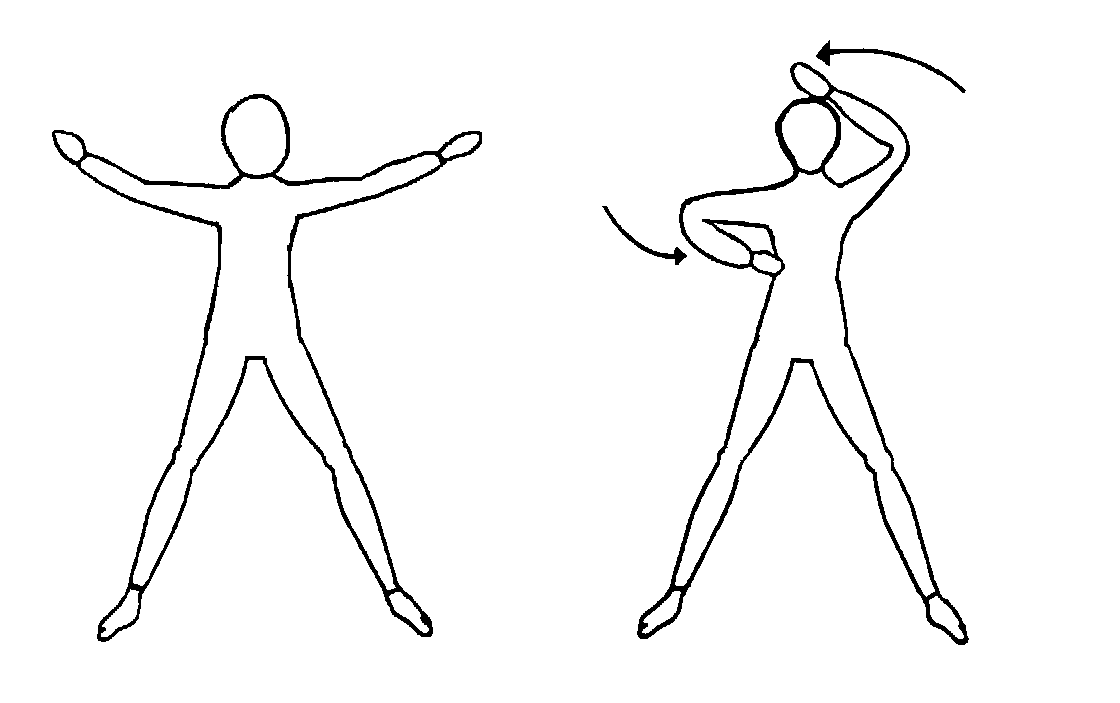
\includegraphics[width=0.7\textwidth]{Harjoitusveto.png}\captionof{figure}{Symmetrinen avausliike}\end{Figure}  

\begin{description}
\item[TAIVUTA (101)] \hfill \\ 
Otetaan X-asento ja taivutus tai delta ja taivutus (jalat lähes suorina). \hfill \\ 
\item[TARTU (102)] \hfill \\ 
vasen käsi kypärän päälle eteen vartalon normaaliksi jatkeeksi ja oikea käsi kahvalle, tiukka ote \hfill \\ 
\item[VEDÄ (103)] \hfill \\ 
veto kahvasta putken tai taskun suuntaan \hfill \\ 
asennon palautus X:ään tai deltaan. \hfill \\ 
\item[101] \hfill \\ 
Aloitetaan laskeminen alusta vedon jälkeen. \hfill \\ 
\end{description}
\begin{description}
\item[102…104] \hfill \\ 
Varjo avautuu ja tehdään sen lopullinen avaaminen. \hfill \\ 
\end{description}
\begin{description}
\item[105] \hfill \\ 
Vilkaistaan olkapään yli tarvittaessa. \hfill \\ 
\end{description}

LENTÄÄ-päätöksen jälkeen laitetaan harjoitusvetokahva pois kädestä (haalarin alle tai rintahihnaan). EI LENNÄ -päätöksen jälkeen pudotetaan harjoitusvetokahva pois ja tehdään varavarjotoimenpiteet. 

\subsection{ Vaaratilanteet }
\label{pl-alkeiskoulutuksen-suoritukset-vaaratilanteet}

\begin{enumerate}[label=\bfseries \arabic*)]
\item  Epästabiili asento: kädet/käsi tai jalat/jalka sisällä --> kaatuu kyljelleen/selälleen --> mahdollista sotkeutua avautuvaan varjoon. 
\item  Veto väärästä kahvasta: päävarjo irtoaa ja varavarjo aukeaa tai varavarjo aukeaa --> varjot voivat sotkeutua toisiinsa. 
\end{enumerate}
\subsection{ Harjoitus }
\label{pl-alkeiskoulutuksen-suoritukset-harjoitus}

\begin{enumerate}[label=\bfseries \arabic*)]
\item  Harjoitellaan suoritusta seuraavasti: 
	\begin{itemize}
	\item  sekunti sekunnilta maassa liikerataharjoituksena 
	\item  sekunti sekunnilta maassa varusteet päällä 
	\item  harjoitusvaljaissa varavarjo- ja vaaratilanteet mukana. 
	\end{itemize}
\item  Annetaan näyte hyppymestarille. 
\end{enumerate}

\end{multicols}\pagebreak\begin{multicols}{2} 

\section{ Itseaukaisu 3'' }
\label{pl-alkeiskoulutuksen-suoritukset-itseaukaisu-3}


Itseaukaisun (IA) tavoitteena on oppia avaamaan laskuvarjo itse. Lisäksi on tunnettava vapaapudotuksen perusteet, osattava poistaa turbulenssi ja osattava pakata itseaukaisuvarjo. Tässä vaiheessa on myös kerrattava varavarjotoimenpiteet ja toiminta apuvarjon yhdyspunoksen tai kantopunoksen kiinnitarttumistilanteissa. 


Itseaukaisuihin pääsy vaatii vähintään kuusi pakkolaukaisuhyppyä, joista kolmella on suoritettu hyväksytty harjoitusveto. Koulutuksen sekä maa- ja valjasharjoittelun jälkeen voidaan lähteä hyppäämään itseaukaisuhyppyjä. Viimeinen harjoitusveto ja ensimmäinen itseaukaisu hypätään samana tai seuraavana kalenterivuorokautena. 


Asennon (X ja taivutus tai delta ja taivutus) ja ajantajun säilyminen sekä korkeuden tarkkailu ovat tärkeitä kaikilla itseaukaisuhypyillä. 

\begin{itemize}
\item  3'' veto 103:lla 
\item  5'' veto 105:llä 
\end{itemize}
\subsection{ Oppimistavoitteet }
\label{pl-alkeiskoulutuksen-suoritukset-oppimistavoitteet}

\begin{enumerate}[label=\bfseries \arabic*)]
\item  Pidä stabiili asento ennen aukaisua ja aukaisun aikana. 
\item  Avaa varjo noin 3 sekunnin sisällä uloshypystä. 
\item  Palauta asento symmetriseksi vedon jälkeen. 
\end{enumerate}
\subsection{ Hyppylennolla }
\label{pl-alkeiskoulutuksen-suoritukset-hyppylennolla}


Varo varusteiden tarttumista koneessa oleviin ulokkeisiin aina koneessa liikkuessasi. Suojaa erityisesti varjojen aukaisukahvoja. Jos takerrut kiinni johonkin, älä revi väkisin vaan ilmoita asiasta hyppymestarille. Vältä turhaa liikkumista. Pidä mahdolliset istuinvyöt kiinni, kunnes hyppymestari aukaisee ne tai antaa luvan aukaisuun. Jos lennon aikana huomaat omissa tai muiden varusteissa jotain poikkeavaa, ilmoita siitä heti hyppymestarille. Keskity omaan hyppyysi. Huomioi muut koneessa olijat äläkä häiritse heidän keskittymistään. Koneen päällikkö on lentäjä, mutta sinun päällikkösi on hyppymestari. 

\subsection{ Hypyn kulku }
\label{pl-alkeiskoulutuksen-suoritukset-hypyn-kulku}

\begin{description}
\item[TAIVUTA (101)] \hfill \\ 
Otetaan X-asento ja taivutus tai delta ja taivutus (jalat lähes suorina). \hfill \\ 
\item[TARTU (102)] \hfill \\ 
vasen käsi kypärän päälle eteen vartalon normaaliksi jatkeeksi ja oikea käsi kahvalle, tiukka ote \hfill \\ 
\item[VEDÄ (103)] \hfill \\ 
veto kahvasta putken tai taskun suuntaan \hfill \\ 
asennon palautus X:ään tai deltaan. \hfill \\ 
\item[101 ] \hfill \\ 
Aloitetaan laskeminen alusta vedon jälkeen. \hfill \\ 
\item[102..104 ] \hfill \\ 
Varjo avautuu ja tehdään sen lopullinen avaaminen. \hfill \\ 
\item[105 ] \hfill \\ 
Vilkaistaan olkapään yli tarvittaessa (turbulenssin poisto). \hfill \\ 
\end{description}

LENTÄÄ-päätöksen jälkeen laitetaan avauskahva pois kädestä (haalarin alle tai rintahihnaan). EI LENNÄ -päätöksen jälkeen pudotetaan avauskahva pois ja tehdään varavarjotoimenpiteet. 


\end{multicols}\pagebreak\begin{multicols}{2} 

\section{ Itseaukaisu 5'' }
\label{pl-alkeiskoulutuksen-suoritukset-itseaukaisu-5}


Tämä on toinen itseaukaisuhyppysi. Irrota streevasta tai ponnista koneesta, laske 101 - 102 - taivuta - tartu - vedä. Kiinnitä edelleen huomiota stabiiliin asentoon, myös vedon jälkeen. Ajantajun on säilyttävä paremmin. 

\subsection{ Oppimistavoitteet }
\label{pl-alkeiskoulutuksen-suoritukset-oppimistavoitteet}

\begin{enumerate}[label=\bfseries \arabic*)]
\item  Pidä stabiili asento ennen aukaisua, aukaisun aikana ja palauta asento symmetriseksi vedon jälkeen. 
\item  Aloita avaustoimenpiteet 4-7 sekunnin sisällä uloshypystä, ja avaa päävarjo. 
\end{enumerate}
\subsection{ Hyppylennolla }
\label{pl-alkeiskoulutuksen-suoritukset-hyppylennolla}

\begin{itemize}
\item Kertaa suoritus mielessäsi 
\item Keskity suoritukseesi 
\item 3X3 -tarkastus ennen hyppyä (\ref{laskuvarjokalusto-ja-hyppyvarusteet-3x3-tarkastus} s.\pageref{laskuvarjokalusto-ja-hyppyvarusteet-3x3-tarkastus}) 
\end{itemize}
\subsection{ Hypyn kulku }
\label{pl-alkeiskoulutuksen-suoritukset-hypyn-kulku}

\begin{description}
\item[TAIVUTA] \hfill \\ 
Tee uloshyppy koneesta ottaen välittömästi ilmavirtaan päästyäsi hyvä taivutus. \hfill \\ 
\item[101] \hfill \\ 
 Säilytä ajantajusi laskemalla.  \hfill \\ 
\item[102 ] \hfill \\ 
Varmistetaan taivutus ja asento. \hfill \\ 
\item[TAIVUTA (103)] \hfill \\ 
Otetaan X-asento ja taivutus tai delta ja taivutus (jalat lähes suorina). \hfill \\ 
\item[TARTU (104)] \hfill \\ 
vasen käsi kypärän päälle eteen vartalon normaaliksi jatkeeksi ja oikea käsi kahvalle, tiukka ote \hfill \\ 
\item[VEDÄ (105)] \hfill \\ 
veto kahvasta putken tai taskun suuntaan \hfill \\ 
asennon palautus X:ään tai deltaan. \hfill \\ 
\item[101 ] \hfill \\ 
Aloitetaan laskeminen alusta vedon jälkeen. \hfill \\ 
\item[102..104 ] \hfill \\ 
Varjo avautuu ja tehdään sen lopullinen avaaminen. \hfill \\ 
\item[105 ] \hfill \\ 
Vilkaistaan olkapään yli tarvittaessa (turbulenssin poisto). \hfill \\ 
\end{description}

LENTÄÄ-päätöksen jälkeen laitetaan avauskahva pois kädestä (haalarin alle tai rintahihnaan). EI LENNÄ -päätöksen jälkeen pudotetaan avauskahva pois ja tehdään varavarjotoimenpiteet. 


\end{multicols}\pagebreak\begin{multicols}{2} 

\section{ 10'' }
\label{pl-alkeiskoulutuksen-suoritukset-10}


Tämä on ensimmäinen hyppysi, jossa vapaapudotusvauhti kasvaa maksimiinsa. Oikea, stabiili ja symmetrinen asento ja hyvä taivutus takaavat hyvän suorituksen. 


Avaustoimenpiteet aloitetaan 1200 metrin korkeudessa mittarin mukaan. Laskemisella säilytetään ajantaju. 

\subsection{ Oppilaan toiminta }
\label{pl-alkeiskoulutuksen-suoritukset-oppilaan-toiminta}

\begin{itemize}
\item Kertaa suoritus mielessäsi 
\item Keskity suoritukseesi 
\item 3X3 -tarkastus ennen hyppyä (\ref{laskuvarjokalusto-ja-hyppyvarusteet-3x3-tarkastus} s.\pageref{laskuvarjokalusto-ja-hyppyvarusteet-3x3-tarkastus}) 
\end{itemize}
\subsection{ Oppimistavoitteet }
\label{pl-alkeiskoulutuksen-suoritukset-oppimistavoitteet}

\begin{enumerate}[label=\bfseries \arabic*)]
\item  Pidä stabiili asento ennen aukaisua, aukaisun aikana ja sen jälkeen.  
\item  Arvioi avauskorkeus mittarin avulla ja aloita avaustoimenpiteet sovitussa korkeudessa. 
\item  Siirry UH-asennosta hypyn aikana perusasentoon. 
\end{enumerate}
\subsection{ Hyppylennolla }
\label{pl-alkeiskoulutuksen-suoritukset-hyppylennolla}

\begin{itemize}
\item Kertaa suoritus mielessäsi 
\item Keskity suoritukseesi 
\item 3X3 -tarkastus ennen hyppyä 
\end{itemize}
\subsection{ Hypyn kulku }
\label{pl-alkeiskoulutuksen-suoritukset-hypyn-kulku}

\begin{description}
\item[TAIVUTA] \hfill \\ 
Tee uloshyppy koneesta ottaen välittömästi ilmavirtaan päästyäsi hyvä taivutus. \hfill \\ 
\item[101..106] \hfill \\ 
 Säilytä ajantajusi laskemalla. \hfill \\ 
 Tarkkaile korkeutta. \hfill \\ 
\item[107] \hfill \\ 
 Vapaapudotusvauhti on maksimissa, rentouta asentoa. \hfill \\ 
\item[1200 metriä] \hfill \\ 
Aloita avaustoimenpiteet. \hfill \\ 
\item[TAIVUTA ] \hfill \\ 
Varmistetaan taivutus ja asento. \hfill \\ 
\item[TARTU] \hfill \\ 
Vasen käsi kypärän päälle eteen vartalon normaaliksi jatkeeksi ja oikea käsi kahvalle, tiukka ote. \hfill \\ 
\item[VEDÄ] \hfill \\ 
Veto kahvasta putken tai taskun suuntaan. \hfill \\ 
Palauta perusasento. \hfill \\ 
\item[101 ] \hfill \\ 
Aloitetaan laskeminen alusta vedon jälkeen. \hfill \\ 
\item[102..104 ] \hfill \\ 
Varjo avautuu ja tehdään sen lopullinen avaaminen. \hfill \\ 
\item[105 ] \hfill \\ 
Vilkaistaan olkapään yli tarvittaessa (turbulenssin poisto). \hfill \\ 
\end{description}

LENTÄÄ-päätöksen jälkeen laitetaan avauskahva pois kädestä (haalarin alle tai rintahihnaan). EI LENNÄ -päätöksen jälkeen pudotetaan avauskahva pois ja tehdään varavarjotoimenpiteet. 

\end{multicols}

\part{Peruskoulutus}\chapter{Yhteenveto: Peruskoulutus}
\label{yhteenveto-peruskoulutus}
\thispagestyle{headings}
\begin{multicols}{2}
\section{ Hyppysuoritukset, NOVA }
\label{yhteenveto-peruskoulutus-hyppysuoritukset-nova}

\begin{itemize}
\item  8'' lyhyt vapaa (\ref{nova-peruskoulutuksen-suoritukset-8} s.\pageref{nova-peruskoulutuksen-suoritukset-8}) 
\item  Kaksi 5'' lyhyttä vapaata (\ref{nova-peruskoulutuksen-suoritukset-5} s.\pageref{nova-peruskoulutuksen-suoritukset-5}) 
\item  Selkälento (\ref{peruskoulutuksen-muut-suoritukset-selkalento} s.\pageref{peruskoulutuksen-muut-suoritukset-selkalento}) 
\item  Liuku (\ref{peruskoulutuksen-muut-suoritukset-liuku} s.\pageref{peruskoulutuksen-muut-suoritukset-liuku}) 
\item  FS-liuku (\ref{peruskoulutuksen-muut-suoritukset-fs-liuku} s.\pageref{peruskoulutuksen-muut-suoritukset-fs-liuku}) 
\end{itemize}
\section{ Hyppysuoritukset, PL }
\label{yhteenveto-peruskoulutus-hyppysuoritukset-pl}

\begin{itemize}
\item  15'' (\ref{pl-peruskoulutuksen-suoritukset-15} s.\pageref{pl-peruskoulutuksen-suoritukset-15}) 
\item  Suora uloshyppy (\ref{pl-peruskoulutuksen-suoritukset-suora-uloshyppy} s.\pageref{pl-peruskoulutuksen-suoritukset-suora-uloshyppy}) 
\item  Sukellusuloshyppy (\ref{pl-peruskoulutuksen-suoritukset-sukellusuloshyppy} s.\pageref{pl-peruskoulutuksen-suoritukset-sukellusuloshyppy}) 
\item  360° käännökset (\ref{pl-peruskoulutuksen-suoritukset-360deg-kaannokset} s.\pageref{pl-peruskoulutuksen-suoritukset-360deg-kaannokset}) 
\item  Tynnyri ja takavoltti (\ref{pl-peruskoulutuksen-suoritukset-tynnyri-ja-takavoltti} s.\pageref{pl-peruskoulutuksen-suoritukset-tynnyri-ja-takavoltti}) 
\item  Selkälento (\ref{peruskoulutuksen-muut-suoritukset-selkalento} s.\pageref{peruskoulutuksen-muut-suoritukset-selkalento}) 
\item  Liuku (\ref{peruskoulutuksen-muut-suoritukset-liuku} s.\pageref{peruskoulutuksen-muut-suoritukset-liuku}) 
\item  FS-liuku (\ref{peruskoulutuksen-muut-suoritukset-fs-liuku} s.\pageref{peruskoulutuksen-muut-suoritukset-fs-liuku}) 
\end{itemize}
\section{ Muut suoritukset }
\label{yhteenveto-peruskoulutus-muut-suoritukset}

\begin{itemize}
\item  5 paikanmääritystä, laskeutuminen kouluttajan osoittamalle alueelle  
\item  Varusteiden tarkastusnäyte 
\item  Jatkokoulutuksen teoriakoe. Opiskeltava alue on luvusta \textit{Yhteenveto: Jatkokoulutus} (\ref{yhteenveto-jatkokoulutus} s.\pageref{yhteenveto-jatkokoulutus}) lukuun \textit{Jatkokoulutuksen suoritukset} (\ref{jatkokoulutuksen-suoritukset} s.\pageref{jatkokoulutuksen-suoritukset}). 
\end{itemize}
\section{ Suoritusten aikarajat }
\label{yhteenveto-peruskoulutus-suoritusten-aikarajat}


Jos peruskoulutuksen aikana oppilaalle tulee 30 vrk tai sitä pidempi hyppytauko, hänen on hypättävä totutteluhyppynä 15'' (tai lyhyempi vapaa, jos kouluttaja näkee tarpeelliseksi) ennen seuraavaa ohjelman mukaista hyppyä. Hyppymestari voi määrätä muitakin suorituksia. 

\end{multicols}

\chapter{Uloshyppytyylit}
\label{uloshyppytyylit}
\thispagestyle{headings}
\begin{multicols}{2}

Uloshyppy ja ensimmäiset 1-2 sekuntia vapaapudotusta ovat ensimmäisillä hypyillä tyypillisesti sellaisia, että hyppääjä ei muista niistä mitään. Kokemuksen karttuessa ajantaju alkaa säilymään koko hyppysuorituksen ajan. Erityisesti hyppyuran alkuvaiheessa hyvä uloshyppy on yhtä kuin hyvä hyppy. Myöhemmin uloshypyn onnistuminen korostuu sekä muodostelmahypyillä että matalilla hypyillä (lyhyet vapaat). Uloshyppytyylistä riippumatta perusperiaate on hyödyntää suhteellista ilmavirtaa halutun asennon ja suunnan saamiseksi ja säilyttämiseksi. 


Uloshyppy on aina arvioitava suoritus ja sen tärkeimmät tekijät ovat ilmavirran suunnan huomioiminen sekä ponnistuksen suunta. Uloshyppyyn on varattava myös aina riittävästi aikaa, mikä on huomioitava uloshyppypaikkaa määriteltäessä. Tavoitteena on hallita kaikki uloshyppytyylit rutiinitasolla ja muistaa koko hyppysuoritus heti uloshypystä maahantuloon asti. 

\section{ Roikkumauloshyppy }
\label{uloshyppytyylit-roikkumauloshyppy}

\subsection{ Streevakone }
\label{uloshyppytyylit-streevakone}

\begin{enumerate}[label=\bfseries \arabic*)]
\item  Kiivetään streevakoneen ulkopuolelle (varoen repun osumista koneeseen) streevaa ja astinlautaa hyväksikäyttäen, rinta koneen etenemissuuntaan. 
\item  Lasketaan jalat yksitellen ilmavirtaan, ei hypätä. 
\item  Roikutaan käsillä noin hartialevyisellä otteella streevasta kiinni pitäen ja otetaan X-asento ja taivutus ilmavirran suuntaisesti. 
\item  Irrotetaan käsien ote yhtäaikaisesti. 
\item  Sitä mukaan kun asento kääntyy vaakatasoon (tyypillisesti noin 5 sekunnin jälkeen) otetaan perusasento. 
\end{enumerate}
\subsection{ Ongelmat }
\label{uloshyppytyylit-ongelmat}

\begin{itemize}
\item  Koukussa olevat jalat aiheuttavat takavoltin. 
\item  Negatiivinen taivutus kaataa asennon selälleen. 
\item  Astinlaudalta ilmavirtaan hyppääminen voi aiheuttaa ennenaikaisen tippumisen. 
\item  Käsillä ponnistaminen kaataa asennon selälleen. 
\end{itemize}
\section{ Suora uloshyppy }
\label{uloshyppytyylit-suora-uloshyppy}


\begin{Figure}\centering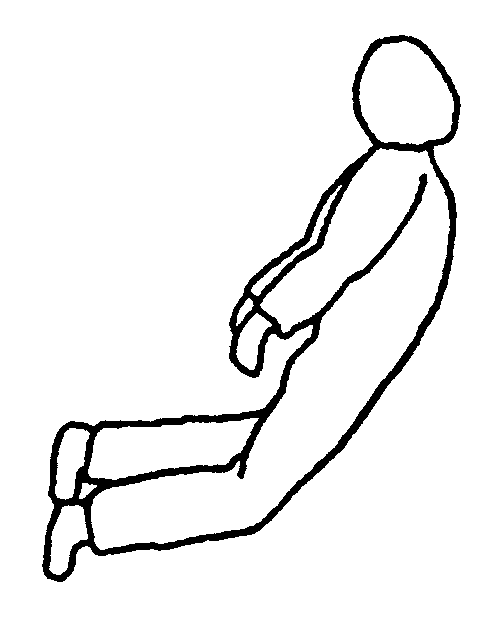
\includegraphics[width=0.7\textwidth]{UH-suora.png}\captionof{figure}{Suora uloshyppy}\end{Figure} 

\subsection{ Streevakone }
\label{uloshyppytyylit-streevakone}

\begin{enumerate}[label=\bfseries \arabic*)]
\item  Vasen jalka astimelle (pyörälle). 
\item  Kädet oviaukon reunalle. 
\item  Kohottaudutaan koneen (varoen repun osumista koneeseen) ulkopuolelle. 
\item  Käännetään rinta koneen etenemissuuntaan. 
\item  Ponnistetaan ilmavirran suuntaan taaksepäin. 
\item  Taivutus, pää taakse, jalat lähes suorina ja kädet taakse delta-asentoon. 
\item  Sitä mukaan kun asento kääntyy vaakatasoon (tyypillisesti noin 5 sekunnin jälkeen) otetaan perusasento. 
\end{enumerate}
\subsection{ Muut koneet }
\label{uloshyppytyylit-muut-koneet}

\begin{enumerate}[label=\bfseries \arabic*)]
\item  Siirrytään oviaukolle (varoen repun osumista koneeseen) kyykkyyn tai seisaalleen. 
\item  Ponnistetaan ilmavirran suuntaan eteenpäin, rinta koneen etenemissuuntaan. 
\item  Taivutus, pää taakse, jalat lähes suorina ja kädet taakse delta-asentoon. 
\item  Sitä mukaan kun asento kääntyy vaakatasoon (tyypillisesti noin 5 sekunnin jälkeen) otetaan perusasento. 
\end{enumerate}
\subsection{ Ongelmat }
\label{uloshyppytyylit-ongelmat}

\begin{enumerate}[label=\bfseries \arabic*)]
\item  Eteen jätetyt kädet aiheuttavat voltin. 
\item  Ponnistus sivulle aiheuttaa kaatumisen kyljelle. 
\item  Löysä uloshyppyasento aiheuttaa kaatumisen selälleen. 
\item  Streeva-koneessa heikko ponnistus voi johtaa osumiseen pyörätelineeseen. 
\end{enumerate}
\section{ Sukellusuloshyppy }
\label{uloshyppytyylit-sukellusuloshyppy}


\begin{Figure}\centering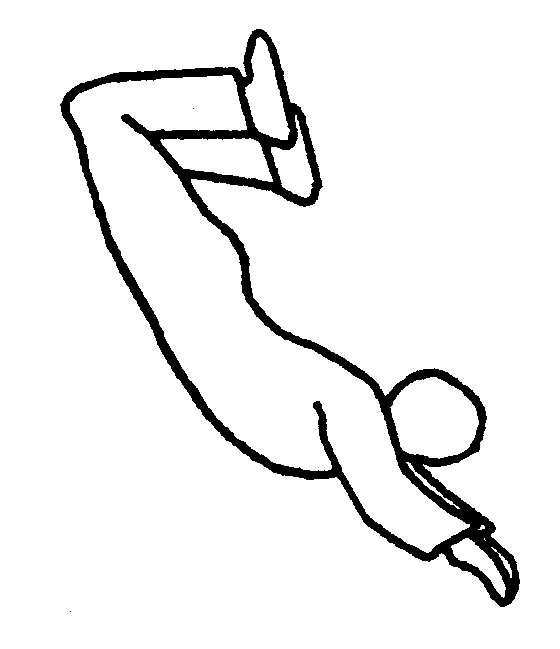
\includegraphics[width=0.7\textwidth]{UH-sukellus.png}\captionof{figure}{Sukellusuloshyppy}\end{Figure} 

\subsection{ Streevakone }
\label{uloshyppytyylit-streevakone}

\begin{enumerate}[label=\bfseries \arabic*)]
\item  Oikea jalka astimelle, varpaat peräsimen suuntaan. 
\item  Kädet oviaukon reunalle. 
\item  Kohottaudutaan (varoen repun osumista koneeseen) koneen ulkopuolelle. 
\item  Käännytään koneen peräsintä kohti. 
\item  Sukelletaan ilmavirran suuntaan taaksepäin, rinta ilmavirtaan. 
\item  Taivutus, pää taakse, jalat koukkuun taakse ja kädet eteen leveälle. 
\item  Sitä mukaan kun asento kääntyy vaakatasoon (tyypillisesti noin 5 sekunnin jälkeen) otetaan perusasento. 
\end{enumerate}
\subsection{ Muut koneet }
\label{uloshyppytyylit-muut-koneet}

\begin{enumerate}[label=\bfseries \arabic*)]
\item  Siirrytään oviaukolle (varoen repun osumista koneeseen) kyykkyyn tai seisaalleen. 
\item  Sukelletaan ilmavirran suuntaan taaksepäin, rinta ilmavirtaan. 
\item  Taivutus, pää taakse, jalat koukkuun taakse ja kädet eteen leveälle. 
\item  Sitä mukaan kun asento kääntyy vaakatasoon (tyypillisesti noin 5 sekunnin jälkeen) otetaan perusasento. 
\end{enumerate}
\subsection{ Ongelmat }
\label{uloshyppytyylit-ongelmat}

\begin{enumerate}[label=\bfseries \arabic*)]
\item  Ponnistus sivulle aiheuttaa kaatumisen kyljelleen. 
\item  Rintamasuunnan ollessa muutoin kuin ilmavirtaan, asento kaatuu. 
\item  Epäsymmetrinen raajojen asento aiheuttaa kääntymistä, voltin tai syöksyn. 
\end{enumerate}
\section{ Ryhmäuloshyppy }
\label{uloshyppytyylit-ryhmauloshyppy}


Uloshypyn toteutus riippuu hyppääjien määrästä ja hyppykoneesta, mutta onnistuakseen uloshypyn täytyy aina olla yhdenaikainen ja hyppääjien lähtöasennon ilmavirran mukainen. Yhdenaikaisuus saadaan uloshyppylaskennalla, jonka yksi hyppääjistä aloittaa (ready) ja johon muut tulevat mukaan (set, go). Oikea lähtöasento, eli vatsan kääntäminen kohti ilmavirtaa, mahdollistaa hyvän lentoasennon heti uloshypystä lähtien. Jos sekä lähtöasento että yhdenaikaisuus epäonnistuvat, ei uloshyppy onnistu. Uloshyppyä tulee harjoitella yhtä paljon kuin itse vapaapudotusta, koska rauhallinen onnistunut hyppy alkaa hyvästä uloshypystä, kun taas epäonnistunut uloshyppy tuhlaa paljon vapaapudotussekunteja. 


Streevalla tai pyörällä istuminen on ehdottomasti \textbf{kielletty}. 


\begin{Figure}\centering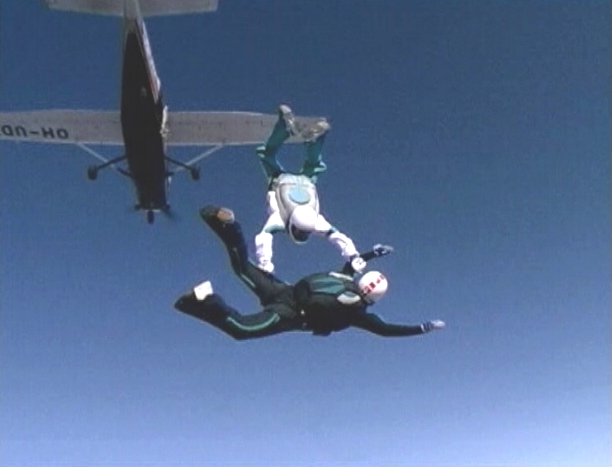
\includegraphics[width=0.95\textwidth]{UH-FS.jpeg}\captionof{figure}{FS-uloshyppy}\end{Figure} 

\section{ Muut uloshypyt }
\label{uloshyppytyylit-muut-uloshypyt}


Hyppääminen muista ilma-aluksista kuten helikoptereista, kuumailmapalloista jne. vaatii aina ennakkoharjoittelua. Perustapana on seisaalta pudottautuminen suoraan alaspäin ilmavirran suuntaan suoralla tai sukellus uloshypyllä. 

\section{ Harjoitus }
\label{uloshyppytyylit-harjoitus}

\begin{enumerate}[label=\bfseries \arabic*)]
\item  Katsotaan eri uloshyppyjä Oppilaan Opas-videolta kouluttajan kanssa. 
\item  Mietitään kouluttajan kanssa miten hyppääjä/hyppääjät hyödyntävät suhteellista ilmavirtaa kussakin uloshyppytyylissä. 
\item  Harjoitellaan omalla hyppykoneella/konemallilla kouluttajan mallisuoritusten mukaan eri uloshyppyjä. 
\item  Omatoiminen harjoittelu koneella/konemallilla ja näyte hyppymestarille suorasta ja sukellusuloshypystä. 
\end{enumerate}
\end{multicols}

\chapter{Perusliikkeet vapaassa}
\label{perusliikkeet-vapaassa}
\thispagestyle{headings}
\begin{multicols}{2}

Vapaapudotuksessa tehtävien liikkeiden edellytyksenä on stabiilin asennon hallitseminen ja ajan- ja korkeudentajun säilyminen koko ajan. Vapaapudotuksessa ongelmat kertaantuvat väkisin tai väärin korjaamalla. Rento asento yhdessä taivutuksen kanssa minimoi ongelmat. Jos ongelma ei poistu korjaamalla, \textbf{avataan varjo välittömästi!} 

\section{ Perusasento }
\label{perusliikkeet-vapaassa-perusasento}


Liikkeiden harjoittelu aloitetaan vasta noin 8 sekuntia uloshypyn jälkeen, kun hyppääjä on saavuttanut lähes täyden vapaapudotusnopeuden. Kaikki liikkeet alkavat perusasennosta ja korkeuden tarkastuksesta. Liikesarjoissa uusi liike aloitetaan vasta, kun edellinen on pysäytetty. Liikkeiden harjoittelu lopetetaan viimeistään 1400 metrin korkeudessa ja keskitytään avaukseen. Siirtyminen perusasentoon tapahtuu 3-5 sekunnin kuluttua uloshypystä. Perusasento on seuraava: 

\begin{itemize}
\item  Lantiossa taivutus ja pää ylös 
\item  Käsivarret 90° kyynärpäästä ja vartalosta 
\item  Jalat levitettyinä, polvet hartioiden tasalla 
\item  Sääret ojennettuina siten, että ilmavirta osuu niihin 
\end{itemize}

\begin{Figure}\centering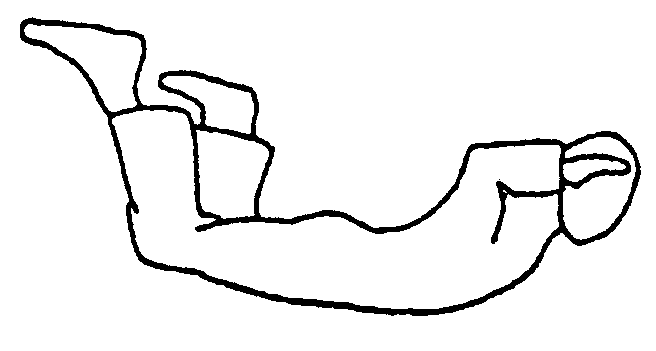
\includegraphics[width=0.7\textwidth]{Asento-perus.png}\captionof{figure}{Vapaapudotuksen perusasento}\end{Figure} 

\section{ Käännös }
\label{perusliikkeet-vapaassa-kaannos}


Käännöksen puoleinen käsi ja hartia painetaan alas. Käännöstä voidaan nopeuttaa vartalon taivutuksella, jalan koukistuksella ja pään kääntämisellä. Käännös tehdään siis seuraavasti: 

\begin{enumerate}[label=\bfseries \arabic*)]
\item  Otetaan kiintopiste 45° edestä maasta, esimerkiksi rakennus. 
\item  Hartialinja painetaan alas halutun käännöksen suuntaan. 
\item  Otetaan perusasento ennen kiintopistettä. 
\item  Vähän ennen kiintopistettä tehdään pieni vastaliike, jotta käännös pysähtyy täsmällisesti. 
\end{enumerate}

\begin{Figure}\centering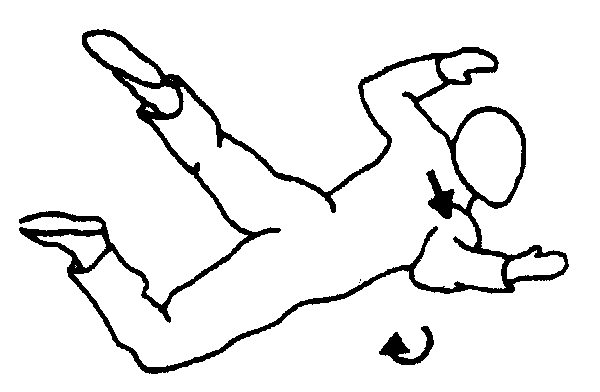
\includegraphics[width=0.7\textwidth]{Asento-kaannos.png}\captionof{figure}{Kääntyminen}\end{Figure} 

\section{ Selkälento }
\label{perusliikkeet-vapaassa-selkalento}


Selkälennon aikana rintahihnassa oleva korkeusmittari ei näytä välttämättä oikein ja vapaapudotusnopeus kasvaa. Jos asennon hallinta menetetään oltaessa selällään (lattakierre), käännetään asento vatsalleen ja otetaan perusasento taivuttamalla. Mikäli asentoa ei saada hallintaan, avataan varjo. Selkälennossa apuvarjo voi irrota löysästä taskustaan tai löysä luuppi voi aiheuttaa varjon ennenaikaisen avautumisen. Selkälento tehdään seuraavasti: 

\begin{enumerate}[label=\bfseries \arabic*)]
\item  Käännetään asento kyljelleen käyttämällä kättä vartalon edessä. 
\item  Taivutetaan samalla asento väärin päin, istuma-asentoon. 
\item  Lennetään muutama sekunti selällään (huomioidaan korkeus). 
\item  Taivutetaan ja käännetään asento käyttämällä kättä vartalossa, jolloin palataan perusasentoon kyljen kautta. 
\end{enumerate}

Palautusta voidaan auttaa ottamalla ensin delta-asento ja vasta kääntymisen jälkeen perusasento. 

\section{ Takavoltti }
\label{perusliikkeet-vapaassa-takavoltti}


Kädet pidetään perusasennossa suorina, hieman sivuille käännettyinä. Jalat laitetaan yhteen ja koukkuun vartalon alle. Painetaan käsillä alaspäin ilmavirtaa vasten. Pysäytys tapahtuu palauttamalla perusasento. Jalkojen nopea ja yhtaikainen tuonti vartalon alle takaa voltin onnistumisen. Käsillä autetaan ympäri menoa ja estetään asennon kallistuminen sivulle. 


Takavoltti tehdään seuraavasti: 

\begin{enumerate}[label=\bfseries \arabic*)]
\item  Vedetään jalat nopeasti yhteen koukkuun. 
\item  Painetaan käsillä alaspäin ilmavirtaa vasten. 
\item  Pään ollessa alaspäin palautetaan perusasento. 
\end{enumerate}

\begin{Figure}\centering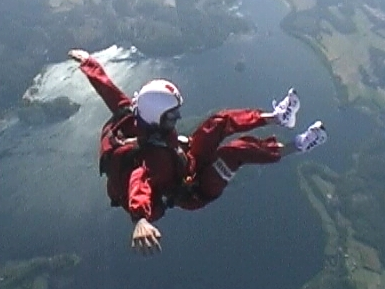
\includegraphics[width=0.9\textwidth]{Selkastabiili.png}\captionof{figure}{Selkälento}\end{Figure} 


\begin{figure*}[]\centering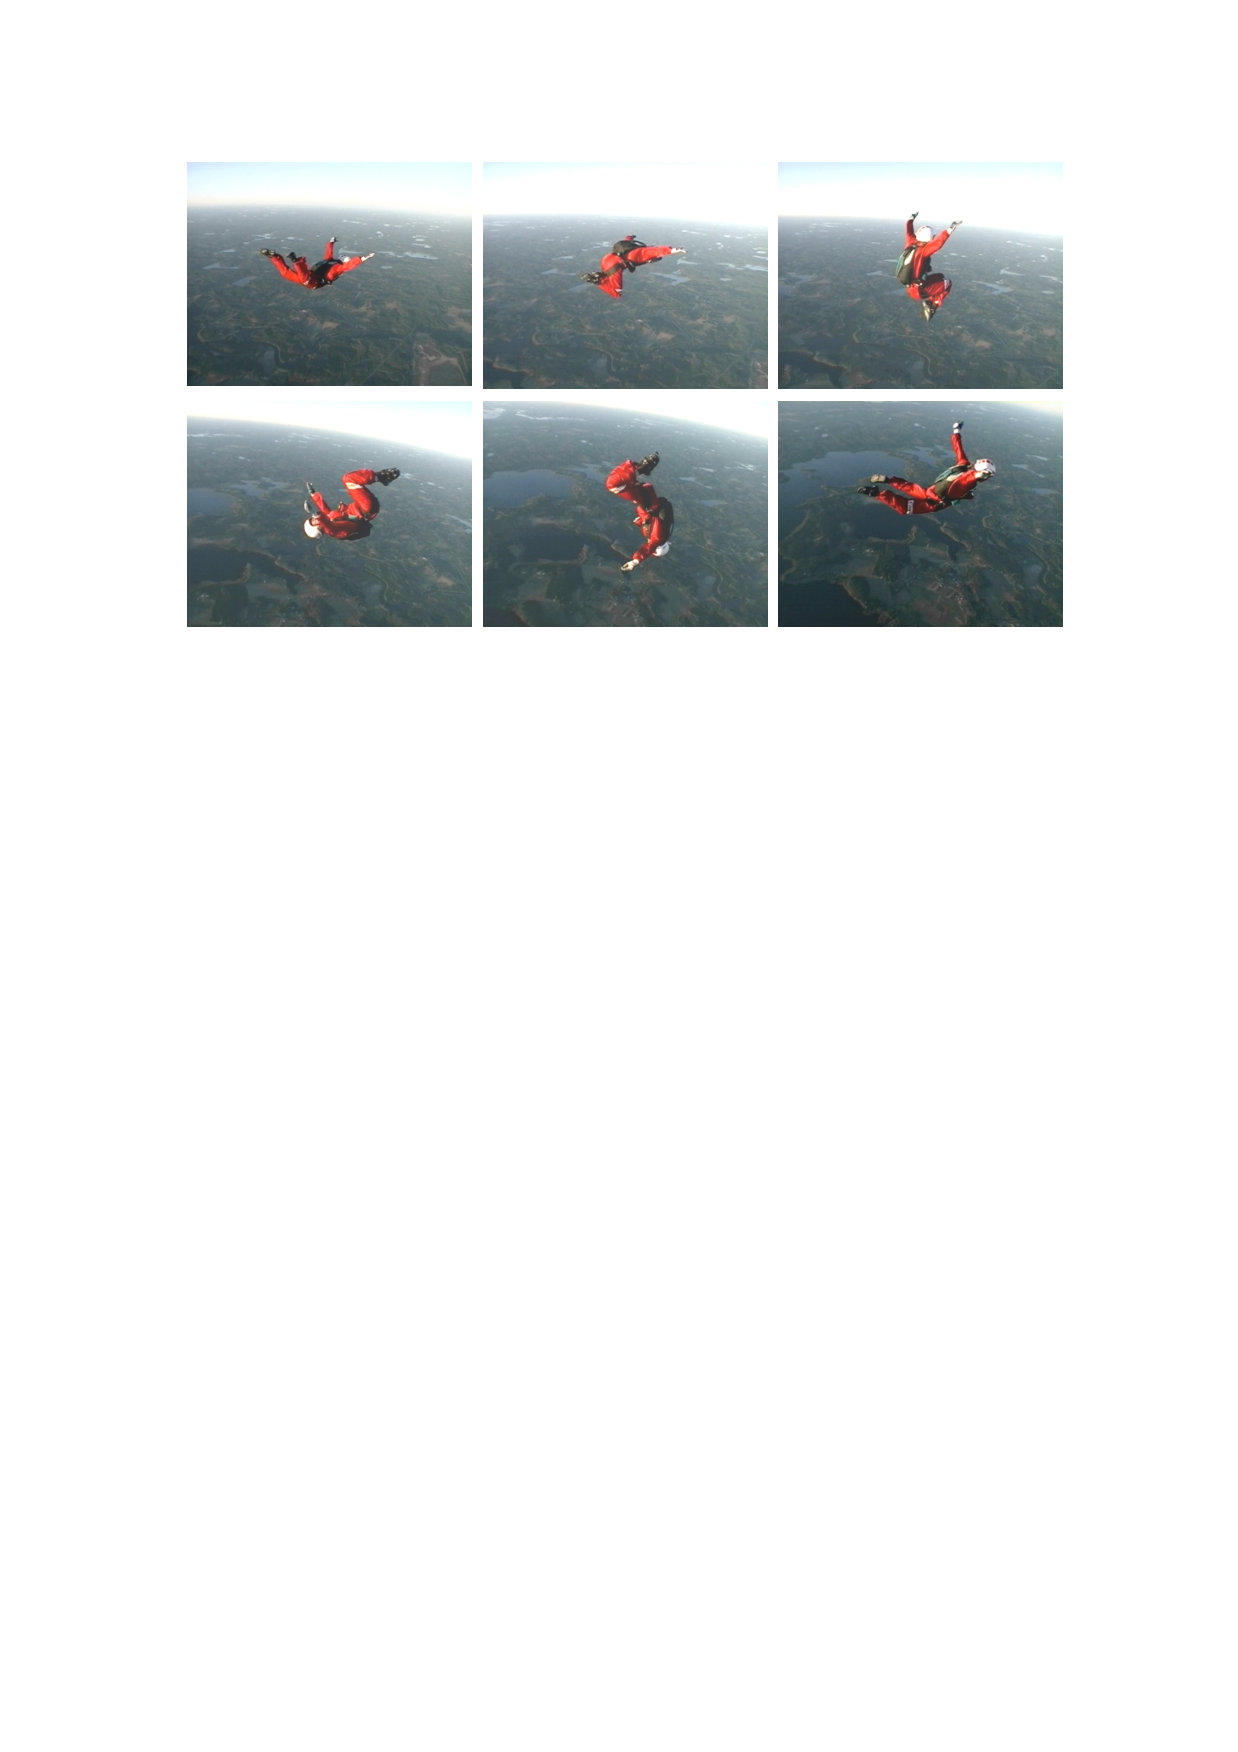
\includegraphics[width=0.95\textwidth]{Takavoltti.pdf}\caption{Takavoltin suoritus}\end{figure*} 

\section{ Tynnyri }
\label{perusliikkeet-vapaassa-tynnyri}


Tynnyri on freeasentojen perusliike, sillä isommilla freekuvilla purun jälkeen liu’uttaessa voidaan tekemällä liu’usta tynnyri tarkastaa vapaa ilmatila ennen avausta. Tynnyrissä on tarkoitus kääntyä vatsaltaan kyljen kautta selälleen ja siitä edelleen täysi kierros takaisin mahalleen. Tynnyri tehdään perusasennosta viemällä toinen käsi vartalon lähelle tai alle ja samalla kääntämällä vartaloa samaan suuntaan vaaka-akselin ympäri. Asennon käännyttyä selälleen jatketaan liikettä kääntymällä toisen kyljen kautta ympäri takaisin perusasentoon. 

\section{ Liuku }
\label{perusliikkeet-vapaassa-liuku}


Liu’un tavoitteena on liikkua vaakatasossa mahdollisimman kauaksi muihin hyppääjiin nähden samalla, kun pudotaan alaspäin. Liuku ei ole siis syöksyä tai tikkaamista. FS-liukuun kuuluvat myös purkumerkki, 180° käännös, liuku vapaaseen suuntaan, liu’un jälkeinen ilmatilan tarkastus sekä avausmerkki ja harjoitusveto. Putoamisnopeus voi kasvaa liu’un aikana. Korkeuden tarkkailu on tärkeää, sillä liu’un pysäytys vaatii myös aikansa. Varjon avaamista suoraan liu’usta ei suositella. Hyvä liuku on ensiarvoisen tärkeä taito laskuvarjohyppääjällä, sillä ainoastaan hyvällä liu’ulla pystyy varmistamaan riittävän välimatkan muihin hyppääjiin purun jälkeen!  Liuku tehdään seuraavasti: 

\begin{enumerate}[label=\bfseries \arabic*)]
\item  Otetaan kiintopiste edestä, maasta. 
\item  Oikaistaan jalat. 
\item  Viedään kädet sivuille taakse, lähelle vartaloa. 
\item  Painetaan olkapäät alas eteen. Hyppääjä on delta-liu’ussa. 
\item  Ohjataan liukusuuntaa kämmenillä. 
\item  Tarkkaillaan korkeutta, muita hyppääjiä sekä liu’utaan kohti kiintopistettä. 
\item  Palautetaan perusasento rauhallisesti ottamalla 
\item  Ensin taivutus = delta-asento 
\item  Palautetaan kädet ja jalat perusasentoon. 
\end{enumerate}

\begin{Figure}\centering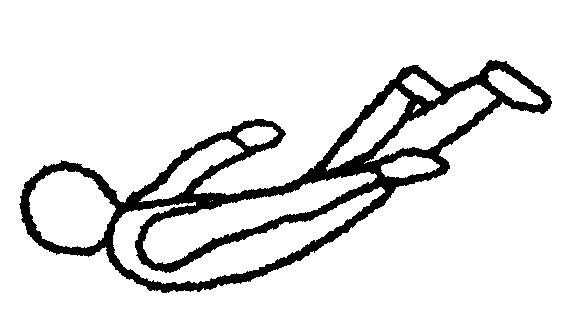
\includegraphics[width=0.7\textwidth]{Asento-deltaliuku.png}\captionof{figure}{Delta-asento}\end{Figure} 


\begin{Figure}\centering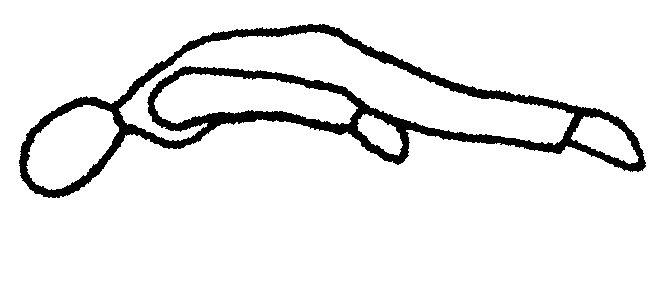
\includegraphics[width=0.7\textwidth]{Asento-liuku.png}\captionof{figure}{Liukuasento}\end{Figure} 


\end{multicols}\pagebreak\begin{multicols}{2} 

\section{ Vaaratilanteet }
\label{perusliikkeet-vapaassa-vaaratilanteet}

\begin{enumerate}[label=\bfseries \arabic*)]
\item  Jäykkyys aiheuttaa asennon heilumista (puun lehden tippumisilmiö). Rentouta asento. 
\item  Epäsymmetrisyys aiheuttaa lattakierrettä. Tee vastaliike. Jos pyöriminen ei pysähdy, avaa varjo heti. 
\end{enumerate}

Lattakierre: 

\begin{itemize}
\item  On holtitonta pyörimistä vaakatasossa 
\item  Aiheutuu epäsymmetrisestä ja jäykästä asennosta tai hallitsemattomasta käännöksestä 
\item  Aiheuttaa asento- ja ajantajun menettämisen 
\item  Pysäytetään rentouttamalla asentoa ja hartialinjan vastaliikkeellä. Jos vastaliike ei auta ja liike ei ole hallinnassa, ota perusasento, taivuta ja avaa varjo heti.  
\end{itemize}

Harjoitukset 

\begin{enumerate}[label=\bfseries \arabic*)]
\item  Katsotaan eri uloshyppyjä Oppilaan Opas -videolta kouluttajan kanssa. 
\item  Harjoitellaan kouluttajan mallien mukaan maassa liike kerrallaan. 
\item  Liikkeiden (delta, liuku ja FS-liuku) harjoittelu laudalla tai vapaapudotusvaljaissa. 
\end{enumerate}
\end{multicols}

\chapter{Sääoppi}
\label{saaoppi}
\thispagestyle{headings}
\begin{multicols}{2}

SIL:n ohjeiden mukaan hyppypaikalla on oltava tuulen suuntaa ja voimakkuutta osoittavat välineet. Lisäksi hyppypaikan puiden, pensaiden, järvien, pilvien, tuulipussin, heitettyjen streamerien ja hyppykoneen sortaman tarkkailu antavat tietoa vallitsevasta säästä. Kokeneet hyppääjät kertovat mielellään, mistä he tietävät tuulen olevan liian voimakas, pilvien olevan liian matalalla tai jos jonnekin paikkaan ei kannata laskeutua pyörteiden takia. Sään tutkiminen ja oppiminen jatkuu koko koulutusajan. Tavoitteena on paikallisten olosuhteiden tunteminen niin, että hyppääjällä on edellytykset hyppypäätöksen tekoon. 

\section{Tuuli}
\label{saaoppi-tuuli}


Tuulet rajoittavat hyppäämistä, sillä tuulen voimistuessa voimistuvat myös pyörteet. Tuulen voimistuessa myös uloshyppypaikan määrittäminen käy vaativammaksi ja ohjaaminen sekä laskeutuminen vaikeutuvat. Laskuvarjohyppääjien tuulirajat määrittävät toiminnalliset rajat, mutta joskus pyörteet voivat olla vaarallisen voimakkaita, vaikka tuulen voimakkuus ei olisikaan yli sallitun. Tuulen suunta eli se suunta mistä päin tuulee ja voimakkuus on tunnettava sekä pinta- että ylätuulten osalta. Tuulen nopeus metreinä sekunnissa saadaan solmuista kertomalla 0,51:llä. Laskuissa kertoimena on helpointa käyttää arvoa 0,5. On syytä muistaa, että jos tuulen nopeus on 16 solmua, se on yli 8 m/s (8,23 m/s). (Samoin 22 kt on 11,32 m/s.) Pintatuuli on tuuli, joka vaikuttaa maanpinnassa (maatuuli). Ylätuulet ovat tuulia, jotka vaikuttavat hyppykorkeuksissa. Pinta- ja ylätuulten suunnan ero on pohjoisella pallonpuoliskolla tyypillisesti oikealle noin 30° maan pyörimisliikkeen takia. Tuulen suunta voi vaihdella kerroksittain. Käsitteellä tuulen yläpuolella tarkoitetaan aluetta laskeutumisalueelta uloshyppypaikalle päin. Vastaavasti käsite tuulen alapuolella tarkoittaa aluetta maalipisteestä poispäin uloshyppypaikkaan nähden. Tuulen nopeus kasvaa ylöspäin mentäessä, maan kitkan pienetessä. Vaikka maassa olisi tyyntä, heti maanpinnan yläpuolella voi tuulla rajusti. Säärintamat (ukkonen) voimistavat tuulia ja lämpötilaerot alueittain (maastoerot) aiheuttavat äkillisiä tuulen suunnan ja voimakkuuden muutoksia. Meren läheisyydessä tuuli voi muuttua kesällä aamupäivällä ja illansuussa täysin päinvastaiseksi (merituuli-ilmiö). Tyynellä hypättäessä loppujarrutuksen oikea ajoittaminen voi olla vaikeaa. 

\subsection{Tuulirajat}
\label{saaoppi-tuulirajat}


Maatuulen nopeuden asettamat rajoitukset laskuvarjohypyille ovat seuraavat: 

\begin{itemize}
\item Itsenäisellä hyppääjällä maatuulen nopeus ei saa ylittää: 
	\begin{itemize}
	\item  A-lisenssihyppääjällä 8 m/s 
	\item  B-lisenssihyppääjällä 11 m/s 
	\item  C-lisenssihyppääjällä 11 m/s 
	\item  D-lisenssihyppääjällä 11 m/s 
	\end{itemize}
\item  Oppilas ei saa hypätä, mikäli maatuulen nopeus ylittää 8 m/s. Tandemoppilas ei saa hypätä, mikäli maatuulen nopeus ylittää 11 m/s. 
\item  Pallovarjoa pää- tai varavarjona käytettäessä maatuulen nopeus ei saa ylittää 8 m/s. 
\end{itemize}
\section{Pilvet}
\label{saaoppi-pilvet}


Laskuvarjohyppäämistä ei saa suorittaa pilvessä tai pilven läpi. Oppilastoiminnan raja on puolipilvinen sää hyppykorkeuden alapuolella. Uloshyppyhetkellä on nähtävä joko maalialue tai uloshyppypaikka. Ilmailumääräyksen OPS M6-1 mukaan tästä voidaan tietyin erityisehdoin poiketa. Tämä asettaa kuitenkin lisävaatimuksia hyppääjille, lentäjälle ja koneen varustukselle. Pilvet jaetaan alapilviin (0–2500 m), keskipilviin (2500–5000 m) ja yläpilviin (yli 5000 m). Pilvet voivat olla esimerkiksi kumpu\mbox{-,} kuuro\mbox{-,} ukkos- tai sumupilviä. Pilvien tyyppejä ei välttämättä tarvitse osata, mutta alasimen mallinen ukkospilvi (Cumulonimbus, Cb) on tunnettava ja hyppytoiminta on keskeytettävä, jos sellainen syntyy kentän läheisyyteen. Pilvet muodostuvat kosteudesta ja ilman epäpuhtauksista, joten vapaapudotuksessa tai varjon varassa pilveen ajautuva hyppääjä kastuu tai saa epämiellyttävän sade- tai raekuuron kasvoilleen. Kostealla säällä, sateen jälkeen ja syksyllä on huomioitava, että kostea ja lämmin ilma kantaa huonommin kuin kuiva ja kylmä ilma. Kosteus vaikuttaa varjon ominaisuuksiin heikentäväksi. 


Jos joudut avaamaan varjon pilvessä: 

\begin{itemize}
\item  Lennä puolijarruilla 
\item  Tee loivaa oikeaa kaarrosta 
\item  Tarkkaile koko ajan etu- ja sivusektoreita 
\item  Huuda ja kuuntele, jos epäilet, ettet ole ainoa pilvessä varjon avannut. 
\end{itemize}
\section{Termiikki}
\label{saaoppi-termiikki}


Termiikki eli nouseva ilmavirtaus muodostuu auringon lämmittämän paikan tai alueen päälle. Tuuli kaataa termiikin, joten se voi olla joko paikan päällä tai alatuulen puolella. Kylmä paikka, esimerkiksi järvi, aiheuttaa puolestaan laskevan ilmavirtauksen. Pilvessä ilma voi virrata sekä ylös- että alaspäin. Nostavat ja laskevat ilmavirtaukset ovat normaalisti 1–8 m/s. Ukkospilvessä virtaukset ovat jopa 30 m/s ylös ja alas. Nyrkkisääntönä voidaan sanoa, että siellä missä on nostava, on myös laskeva. Tämä on huomioitava kuumana kesäpäivänä suunniteltaessa laskeutumiskuvioita. Hyppykentällä virtauksia aiheuttavat mm. maalialueen hiekka, kiitotiet ja kynnetyt pellot. Virtaukset tuntuvat varjossa epämiellyttävänä tärinänä, heilumisena ja kääntymisenä. Lisäksi varjo voi tukahtua, nousta, vajota tai jopa sakata. 

\section{Turbulenssi}
\label{saaoppi-turbulenssi}


Turbulenssi muodostuu tuulen ja esteen yhteisvaikutuksesta ja sitä ilmenee myös tuulikerrostumien rajapinnoissa. Se voi olla voimakas, terävä, nostava tai laskeva, riippuen esteen muodosta ja koosta sekä tuulen voimakkuudesta. Rinnetuuli on aina turbulenttista. Turbulenssi aiheuttaa varjolle samat oireet kuin nostava ja laskeva ilmavirtaus, joten paikallisten turbulenssien tunteminen on tärkeää laskeutumiskuvioita suunniteltaessa. Voimakas turbulenssi voi tyhjentää kuvun osittain tai jopa kokonaan. Tyhjentynyt kupu täyttyy uudestaan, kun kupu saavuttaa oikean kohtauskulman ilmavirtaan nähden. Turbulenssin alla on usein tyyni kohta, joten loppuvedon tekeminen oikea-aikaisesti voi olla vaikeaa. Turbulenttisella säällä lentäminen ja hyppääminen on aina riskialtista ja sitä pitää välttää, vaikkei tuulen voimakkuus olisikaan yli tuulirajojen! Varjoja ei ole suunniteltu toimimaan turbulenttisessa kelissä! Jos kuitenkin syystä tai toisesta joudut varjollasi turbulenttiseen keliin, lennä täydessä liidossa. Liian suurilla jarruilla lentäminen saattaa aiheuttaa kuvun sakkaamisen pyörteen vaikutuksesta. Pyörteitä voi välttää laskeutumalla tarpeeksi kauas reunaesteistä ja esimerkiksi hiekan reunasta, jossa virtausten suunnat muuttuvat. 

\section{Lämpötila}
\label{saaoppi-lampotila}


Ilman lämpötila laskee ylöspäin mennessä n. 6,5 °C / 1000 m. Arvo on epätarkka ja siihen vaikuttavat inversiot, säärintamat sekä ilmanpaineen paikalliset vaihtelut. Laskuvarjohyppääjän kannattaa käyttää hanskoja, kun lämpötila hypyn aikana laskee alle nollan. Oppilailla käsineet ovat pakolliset. Vaikka maassa olisikin lämmintä, hyppykorkeudella voi olla jo pakkasta. Jos maassa on +10 °C lämmintä, voi kahden kilometrin hyppykorkeudella olla jo pakkasta. Jos maassa on +10 °C, lämpötila on kahden kilometrin korkeudessa tyypillisesti noin –3 °C. On huomioitava, että kolmen kilometrin korkeudessa on usein pakkasta. 

\section{Käytännössä}
\label{saaoppi-kaytannossa}


Parhaat hyppykelit Suomessa ovat alku- ja loppukesällä sekä aamulla ja illalla. Tällöin säätekijöiden aiheuttamat muutokset ilmatilassa ovat pienimmillään. Tuuli on heikko, aurinko ei aiheuta nostavia eikä laskevia ja ilmanpaine sekä kosteus ovat ihanteelliset. Säätiedot on aina varmistettava ennen hyppypäätöksen tekoa. Lentosääaseman tiedot, teksti-TV:n tiedot tai mittareilla mitatut arvot ovat aina ehdottomia epävarmoissa tilanteissa. Ne eivät sulje toisiaan pois vaan varmentavat niitä. On muistettava, että taivaalle pääsy ei takaa onnistunutta hyppyä, vaan turvallinen alastulo. 


Lentosääsanomia saadaan mm. seuraavasti: 

\begin{itemize}
\item  Internet (mm. \url{http://www.ilmailusaa.fi/} ) 
\item  Lentosääaseman automaattitiedotus radiolla ja puhelimella 
\item  Sääsanomat YLE Teksti-TV s. 428 ja 429 (myös \url{http://www.yle.fi/tekstitv/html/P428_01.html} ) 
\end{itemize}
\section{ METAR-sanomat }
\label{saaoppi-metar-sanomat}


METAR-sanoma on ilmaliikenteen käyttöön tarkoitettu sääsanoma, joka laaditaan lentopaikan sääasemalla. Metar kertoo lentoasemalla vallitsevan säätilan. Metareita laaditaan pääsääntöisesti kaikilla lentopaikoilla, joille on säännöllistä liikennettä. Suomessa Metar luodaan näiltä lentoasemilta 30 minuutin välein, 20 minuuttia ja 50 minuuttia yli jokaisen tunnin. 


EFTU 231250Z 27006KT 9999 SCT055 FEW080 08/04 Q1015 


Tämä viesti voidaan jakaa osioihin ja tulkita sen perusteella. Metar-viestin pääosiot ovat: 

\begin{itemize}
\item  EFTU Sääasema lentopaikan ICAO-koodilla; Eurooppa, Finland, Turku 
\item  231250Z Aika (UTC) Päivä kuluvaa kuukautta sekä kellonaika UTC-ajassa ilmaistuna  
\item  27006KT Tuulen suunta asteina ja nopeus solmuina, 270 astetta, 3 m/s  
\item  9999 Näkyvyys metreinä, yli 10 km 
\item  SCT055 Pilvien määrä sekä korkeus 
\item  FEW080 Pilvien äärä sekä korkeus  
\item  08/04 Lämpötila ja kastepiste celsiusasteina  
\item  Q1015 Ilmanpaine millibareina / hehtopascaleina  
\item  Lisätiedot ja mahdolliset muut huomioitavat asiat kerrotaan Metarin lopussa  
\end{itemize}

Metar-sanomassa tuulen suunta ilmoitetaan kolmella numerolla, lähimpään 10 asteeseen pyöristettynä. Tuulen nopeuden yksikkönä käytetään solmua (KT). Tuulen ollessa tyyni, ilmoitetaan se metar-sanomassa 00000KT. 

\begin{itemize}
\item  VRB02KT: Suunnaltaan vaihtelevaa tuulta, tuulen nopeus 1 m/s. 
\item  18010KT: Tuulen suunta on etelästä (180 astetta) ja tuulen nopeus on 5 m/s. 
\item  22015G28KT: Tuulen suunta on 220 astetta, keskituulen nopeus 7,5 m/s ja puuskissa 14 m/s. 
\item  35014KT 310V030: Tuulen suunta vaihtelee lentopaikalla siten, ettei keskituulen suuntaa voi määrätä ja keskituulen nopeus on 7 m/s. Tuulen suunnan vaihteluväli on 310 astetta ja 030 astetta. 
\end{itemize}

Metar-sanomassa ilmoitetaan sääilmiöt kuten sumu, sade, lumisade, ukkonen ja muut vastaavat säähän vaikuttavat tekijät.  


Esimerkkejä vallitsevan sään ilmoittamisesta: 

\begin{itemize}
\item  TS: ukkosta ilman sadetta 
\item  TSRA: ukkosta ja vesisadetta 
\item  -RABR: heikkoa vesisadetta ja utua 
\item  FG: sumua 
\item  MIFG: matalaa sumua 
\item  -DZBR: heikkoa tihkusadetta ja utua 
\end{itemize}

Metar-sanomassa pilven alaraja ilmoitetaan lyhennetysti jättämällä korkeuden kaksi viimeistä nollaa pois. Esimerkiksi pilven alaraja 300 ft kirjoitetaan METARissa 003, 3000 ft kirjoitetaan 030 ja 30000 ft kirjoitetaan 300. Korkeus ilmoitetaan maanpinnasta. 


Näkyvä taivas jaetaan pilvisyyttä ilmoitettaessa kahdeksaan osaan. Pilvisyys ilmoitetaan kolmen kirjaimen tunnuksella, joka kertoo kuinka monta kahdeksasosaa taivaasta on pilven peitossa kyseisessä korkeudessa: 

\begin{itemize}
\item  0/8 SKC = sky clear (pilvetöntä) 
\item  1/8-2/8 FEW = few (muutamia pilviä)  
\item  3/8-4/8 SCT = scattered (hajanaisia pilviä)  
\item  5/8-7/8 BKN = broken (melkein pilvistä)  
\item  8/8 OVC = overcast (täysin pilvistä) 
\end{itemize}

Pilvestä voidaan ilmoittaa myös lisämääreet CB ja TCU: 

\begin{itemize}
\item  CB - Cumulonimbus, ukkospilvi 
\item  TCU - Towering Cumulus, nouseva cumuluspilvi 
\end{itemize}

Esimerkkejä pilvien ilmoittamisesta: 

\begin{itemize}
\item  FEW007 - vähän pilviä 700 ft korkeudella maanpinnasta. 
\item  SCT020 - 3/8 taivaasta pilvessä 2000 ft korkeudella 
\item  BKN080 - 5/8 taivaasta pilvessä 8000 ft korkeudella. 
\item  OVC003 - täyskatto (8/8) pilviä 300 ft korkeudella. 
\end{itemize}

Koodisana CAVOK on lyhenne englannin kielen sanoista ''Ceiling And Visibility OK''. Sitä käytetään, mikäli kaikki seuraavat ehdot ovat voimassa samanaikaisesti:  

\begin{itemize}
\item  Näkyvyys on 10 km tai enemmän. 
\item  Alueella ei ole pilviä 1500 m (5000 ft) alapuolella eikä CB- tai TCU-pilviä havaita.  
\item  Ei esiinny merkittäviä sääilmiöitä kuten ukkosta, sadetta tai sumua. 
\end{itemize}
\section{ GAFOR-sanomat }
\label{saaoppi-gafor-sanomat}


Suomi on GAFOR-alue-ennusteiden osalta jaettu kolmeen osaan. GAFOR-sanomassa käytetään samoja lyhenteitä kuin METAR-sanomassa. Hyppääjien kannalta kiinnostavinta GAFOR-sanomassa on tuuliennusteet sekä 2000 ft että 5000 ft korkeudelle. Näitä tuulitietoja voidaan käyttää uloshyppypaikan määrityksessä. 


FBFI42 EFRO 121000 


GA-FCST FOR AREAS 21/25 VALID 0312 UTC 


WX AURINKOISTA JA PILVETÖNTÄ. 


PÄIVÄN MITTAAN ODOTETTAVISSA 


HELLELÄMPÖTILOJA KOKO ALUEELLA. 


WINDS 


SFC 21/23 270-310 / 05-10 KT 24/25 010-030 / 03-06 KT 


2000 FT 300-320 / 15-20 KT 


5000 FT 330 / 25 KT 


0-C LEVEL FL120 


ICE NIL TURB NIL 


GAFOR EFRO 1218 BBBB 21/25 O 


Esimerkkipauksessa kyse on Itä-Suomen alue-ennusteesta. 


Sanoma on voimassa alueilla 21-25 (Utin lentokenttä sijaitsee alueella 22), ja aikavälillä 3.00-12.00 UTC-aikaa. GAFORit laaditaan joka vuorokausi samoille yhdeksän tunnin aikaväleille, joten 0312-sanoma on siis aamu/päiväennuste, ja 1221-sanoma on iltapäivä/iltaennuste. 


WX (Weather eXplanation, sään kuvaus)- tunnuksesta eteenpäin kuvataan parilla-kolmella rivillä selkeästi sanoman voimassaoloaikana vallitseva tai lähitunteina odotettavissa oleva sää. Joskus WX-osassa kerrotaan myös seuraavan päivän ennuste. 


Tuulitietojen alkaminen ilmaistaan sanomassa tunnuksella WINDS (tuulet). Mikäli kerrostuulien yhteydessä ei ole erillistä alueisiin jakoa, lukee WINDS-tunnuksen perässä monesti 21/25, jolloin kaikki tiedot koskevat koko Itä-Suomen aluetta. Tuulitiedot on aina jaettu kolmeen osaan, eli on ilmoitettu tuulet: 

\begin{itemize}
\item  Maanpinnan läheisyydessä (SFC, surface)  
\item  2000 jalan (600 metrin) korkeudella   
\item  5000 jalan (1500 metrin) korkeudella.  
\end{itemize}

Eri kerroksien tuulitiedot on toisinaan jaettu alueisiin, kuten tässä maatuuliosa. Maatuuliennusteen (SFC) ensimmäinen osa koskee tässä tapauksessa alueita 21/23 eli alueita 21, 22 ja 23. Aluemäärityksen jälkeen ilmoitetaan tuulen suunnan vaihteluväli asteina. 270-310 tarkoittaa siis, että tuulen suunta vaihtelee välillä 270 ja 310 astetta. Kautta-viivan jälkeen annetaan tuulen nopeus tai nopeuden vaihteluväli solmuina (KT, knots). 05-10 KT tarkoittaa siis, että tuulen keskimääräinen voimakkuus on 5 - 10 solmua (2,5 - 5 metriä sekunnissa). Nämä lukemat eivät kerro maatuulen huippuarvoista, jotka saadaan selville kerhon tuulimittarilla tai sääasemalta. 


Maatuulikoodin toinen osa 24/25 010-030 / 03-06 KT kertoo vastaavat tiedot alueille 24 ja 25. 


2000 FT:n (600 metriä) tuulitiedoissa ei ole tällä kertaa erillistä alueisiin jakoa, jolloin ne koskevat koko Itä-Suomen aluetta. 2000 FT 300-320 / 15-20 KT tarkoittaa siis, että 600 metrin korkeudessa tuulen suunta vaihtelee välillä 300-320 astetta, ja voimakkuus välillä 15-20 solmua (7,5 - 10 metriä sekunnissa). 


5000 FT 330 / 25 KT tarkoittaa, että 1500 metrin korkeudessa tuulee suunnasta 330 astetta 25 solmun voimakkuudella (12,5 metriä sekunnissa). 


SFC\mbox{-,} 2000 ft- ja 5000 ft-tuulitiedoilla voi yleensä riittävällä tarkkuudella määritellä jopa 4000 m:n UH-paikan. Erityisesti 5000 ft:n tuulitietoja voidaan käyttää ajautuman laskemiseen korkeusvälillä noin 1000-4000 m, sillä noilla korkeuksilla ei juurikaan ole tuuliolosuhteisiin vaikuttavia häiriötekijöitä. 


Satunnaisesti GAFORin tuulitiedoissa mukana oleva BECMG-lyhenne (Becoming, tulossa) kellonaika- ja tuulitietoineen tarkoittaa, että sanoman voimassaoloaikana on odotettavissa merkittäviä tuulen suunnan tai nopeuden muutoksia. Tämä saattaa merkitä esimerkiksi säärintaman lähestymistä, ja tällöin GAFORista luettaviin tuulitietoihin tulee suhtautua kriittisesti. 


0-C LEVEL-tunnuksella alkava rivi kertoo, missä korkeudessa lämpötila vaihtuu pakkasen puolelle ylöspäin mentäessä. Korkeus on ilmaistu kolmella numerolla lentopintana (FL, Flight Level), joka on lentoliikenteessä käytetty ilmanpaineesta riippuva suhteellinen korkeus. Korkeus voidaan kuitenkin tässä tapauksessa karkeasti muuttaa metreiksi ottamatta huomioon ilmanpaineen vaikutusta. Tällä kertaa lämpötilan nollaraja on siis suunnilleen korkeudella 120 sataa eli 12000 jalkaa (3660 metriä). Yksi jalka on 0,3048 metriä. Talvella nollarajatiedolla ei yleensä ole merkitystä, sillä lämpötila on monesti pakkasen puolella heti maanpinnasta lähtien. Tällöin 0-C LEVELin jälkeen saattaa lukea esim. NIL (No information, ei tietoa), NEAR SFC (lähellä maanpintaa) tai GND (Ground, maanpinnan tasalla). 


GAFOR-sanoman parilla viimeisellä rivillä kerrotaan esimerkiksi jäätämisestä ja yläkerrosten turbulenssista, sekä esitetään lyhyt koodi lentosääluokista. 

\section{Harjoitus}
\label{saaoppi-harjoitus}

\begin{enumerate}[label=\bfseries \arabic*)]
\item  Tutustutaan internetin ilmailusääsivuihin: 
	\begin{itemize}
	\item  METAR = vallitseva sää lentopaikalla 
	\item  TAF = sääennuste lentopaikalla 
	\item  GAFOR = alue-ennuste. 
	\end{itemize}
\item  Etsitään maastokartalta kenttäalueen ympäriltä pyörteitä ja nostavia ilmavirtauksia aiheuttavia kohteita. 
\item  Tutustutaan kentän nyrkkisääntöihin tuulen ja pilvien lukemiseksi ilman mittareita.  
\item  Selvitetään laskuvarjohyppääjien tuulirajat. 
\end{enumerate}
\end{multicols}

\chapter{Uloshyppypaikan määritys}
\label{uloshyppypaikan-maaritys}
\thispagestyle{headings}
\begin{multicols}{2}

Uloshyppypaikka määritetään laskemalla yhteen ajautuma varjon varassa sekä ajautuma vapaapudotuksessa. Näiden avulla saadaan selville sijainti ylätuulen puolella. Tämän paikan päällä lentokoneesta poistuva hyppääjä pääsee kaikkein varmimmin laskeutumisalueelle. Uloshyppypaikka ja hyppylinja määritetään aina toiminnan alkaessa. Jos epäillään olosuhteiden muuttuneen, on uloshyppypaikka määritettävä uudelleen. 


Peruskoulutukseen kuuluu vähintään viisi itsenäistä uloshyppypaikan määritystä. Laskeutumisen on tapahduttava kouluttajan määräämälle alueelle. 


Tässä luvussa annetaan ohjeellisia lukuja, joita voidaan käyttää UH-paikan määritykseen. Hyppääjät käyttävät kuitenkin hyvin vaihtelevaa varjokalustoa, ja paikanmääritykseen käytettyjen tuuliennusteiden tarkkuus vaihtelee. Arvioitua UH-paikkaa onkin syytä korjata jos hypättäessä osoittautuu, että laskeutumisalueelle on hankala päästä. 


Myös maassaolijat voivat tehdä näköhavaintoja esimerkiksi koneen sortamisesta hyppylinjalla. Näiden havaintojen avulla he voivat päättää oman uloshyppypaikkansa. Lisäksi kannattaa tarkkailla, missä hyppääjien varjot aukeavat maatuuleen nähden ja pääsevätkö hyppääjät helposti laskeutumisalueelle. Ajautuman arvioinnin tärkeys korostuu, jos laskeutumisalue on pieni, ilmassa on paljon muuta liikennettä tai tuuli on kova. 

\section{ Ajautuminen tuulen mukana }
\label{uloshyppypaikan-maaritys-ajautuminen-tuulen-mukana}


Vapaapudotuksen ja varjon ohjailun aikana tapahtuvan ajautumisen laskeminen on mahdollista, jos tunnetaan tuulet eri kerroksissa maanpinnan ja hyppykorkeuden välillä (ajautuma = tuulen nopeus m/s * pudottu aika s). Ylätuulet voidaan selvittää kysymällä tuulitiedot lentosääasemalta tai katsomalla ennusteista. Lisäksi tuulitietoja eri korkeuksista voidaan saada lentäjältä, mikäli lentokoneessa on GPS-laite. Tuulitietojen perusteella voidaan laskea ajautuman matka ja suunta tai arvioida ne riittävällä tarkkuudella. Tuulitietojen lisäksi on arvioitava eri ilmakerroksissa vietetty aika: 

\begin{itemize}
\item  Vapaapudotuksen ajaksi arvioidaan 50 sekuntia. 
\item  Hyppääjä vajoaa varjon varassa keskimäärin 5 m/s. 
\item  Varjon voidaan odottaa olevan täysin lentävä 800–1000 metrin korkeudessa. 
\item  Varjon varassa vietetyksi ajaksi saadaan siis noin 3 minuuttia. (180 s) 
\end{itemize}

Seuraavaan taulukkoon on laskettu yllä olevilla oletuksilla (lähimpään sataan metriin pyöristettyjä) ajautumia varjon varassa ja vapaapudotuksessa erilaisissa tuulissa. 

\begin{tabular}[]{|l|p{2.4cm}|l|}
\hline
 \textbf{tuuli (kt)} &  \textbf{varjon varassa (m)} &  \textbf{vapaassa (m)}
\\ \hline
 5 &  500 &  100
\\ \hline
 10 &  900 &  300
\\ \hline
 15 &  1400 &  400
\\ \hline
 20 &  1900 &  500
\\ \hline
 25 &  2300 &  600
\\ \hline
 30 &  2800 &  800
\\ \hline
 35 &  3200 &  900
\\ \hline
\end{tabular}
\subsection{ Ajautuminen varjon varassa }
\label{uloshyppypaikan-maaritys-ajautuminen-varjon-varassa}


Varjon varassa tapahtuvan ajautumisen laskemiseksi tarvitaan sekä avauskorkeuden että maatuulen tuulitiedot: nopeus ja suunta. Maatuuli voidaan myös jättää huomiotta ja käyttää vain tuulen nopeutta ja suuntaa esimerkiksi korkeuksissa 1000 ft ja 2000 ft. Tuulen suunnasta ja nopeudesta eri pinnoilla voidaan ottaa keskiarvot. 


Esimerkki ajautuman laskemisesta: 

\begin{tabular}[]{|l|r|r|}
\hline
 \textbf{Korkeus (ft)} &  \textbf{Suunta} &  \textbf{Nopeus (kt)}
\\ \hline
 2000 &  250 &  10
\\ \hline
 Pinta &  230 &  5
\\ \hline
 \textit{Keskiarvo} &  \textit{240} &  \textit{7,5}
\\ \hline
\end{tabular}

Ajautumaksi varjon varassa saadaan 700 metriä. Avauspaikka on siis 0,7 kilometrin etäisyydellä laskeutumisalueelta suuntaan 240 astetta. 

\subsection{ Ajautuminen vapaapudotuksessa }
\label{uloshyppypaikan-maaritys-ajautuminen-vapaapudotuksessa}


Vapaapudotuksessa tapahtuvan ajautumisen laskemiseen käytetään tuulitietoja avauskorkeuden ja uloshyppykorkeuden välillä.  


Esimerkki vapaapudotuksen ajautuman laskemiseen. 

\begin{tabular}[]{|l|r|r|}
\hline
 \textbf{Korkeus (ft)} &  \textbf{Suunta} &  \textbf{Nopeus (kt)}
\\ \hline
 12000 &  290 &  20
\\ \hline
 9000 &  270 &  15
\\ \hline
 6000 &  260 &  15
\\ \hline
 3000 &  250  &  10
\\ \hline
 \textit{Keskiarvo} &  \textit{270} &  \textit{15}
\\ \hline
\end{tabular}

Ajautumaksi vapaassa saadaan 400 metriä. Uloshyppypaikka sijaitsee siis 0,4 kilometriä avauspaikasta suuntaan 270. 


Uloshyppypaikka valitaan ajautuman verran tuulen yläpuolelta laskeutumisalueeseen nähden. Lentäjälle ja muille hyppääjille näytetään paikka koneessa olevalta kartalta tai kerrotaan paikka sanallisesti. 


\begin{Figure}\centering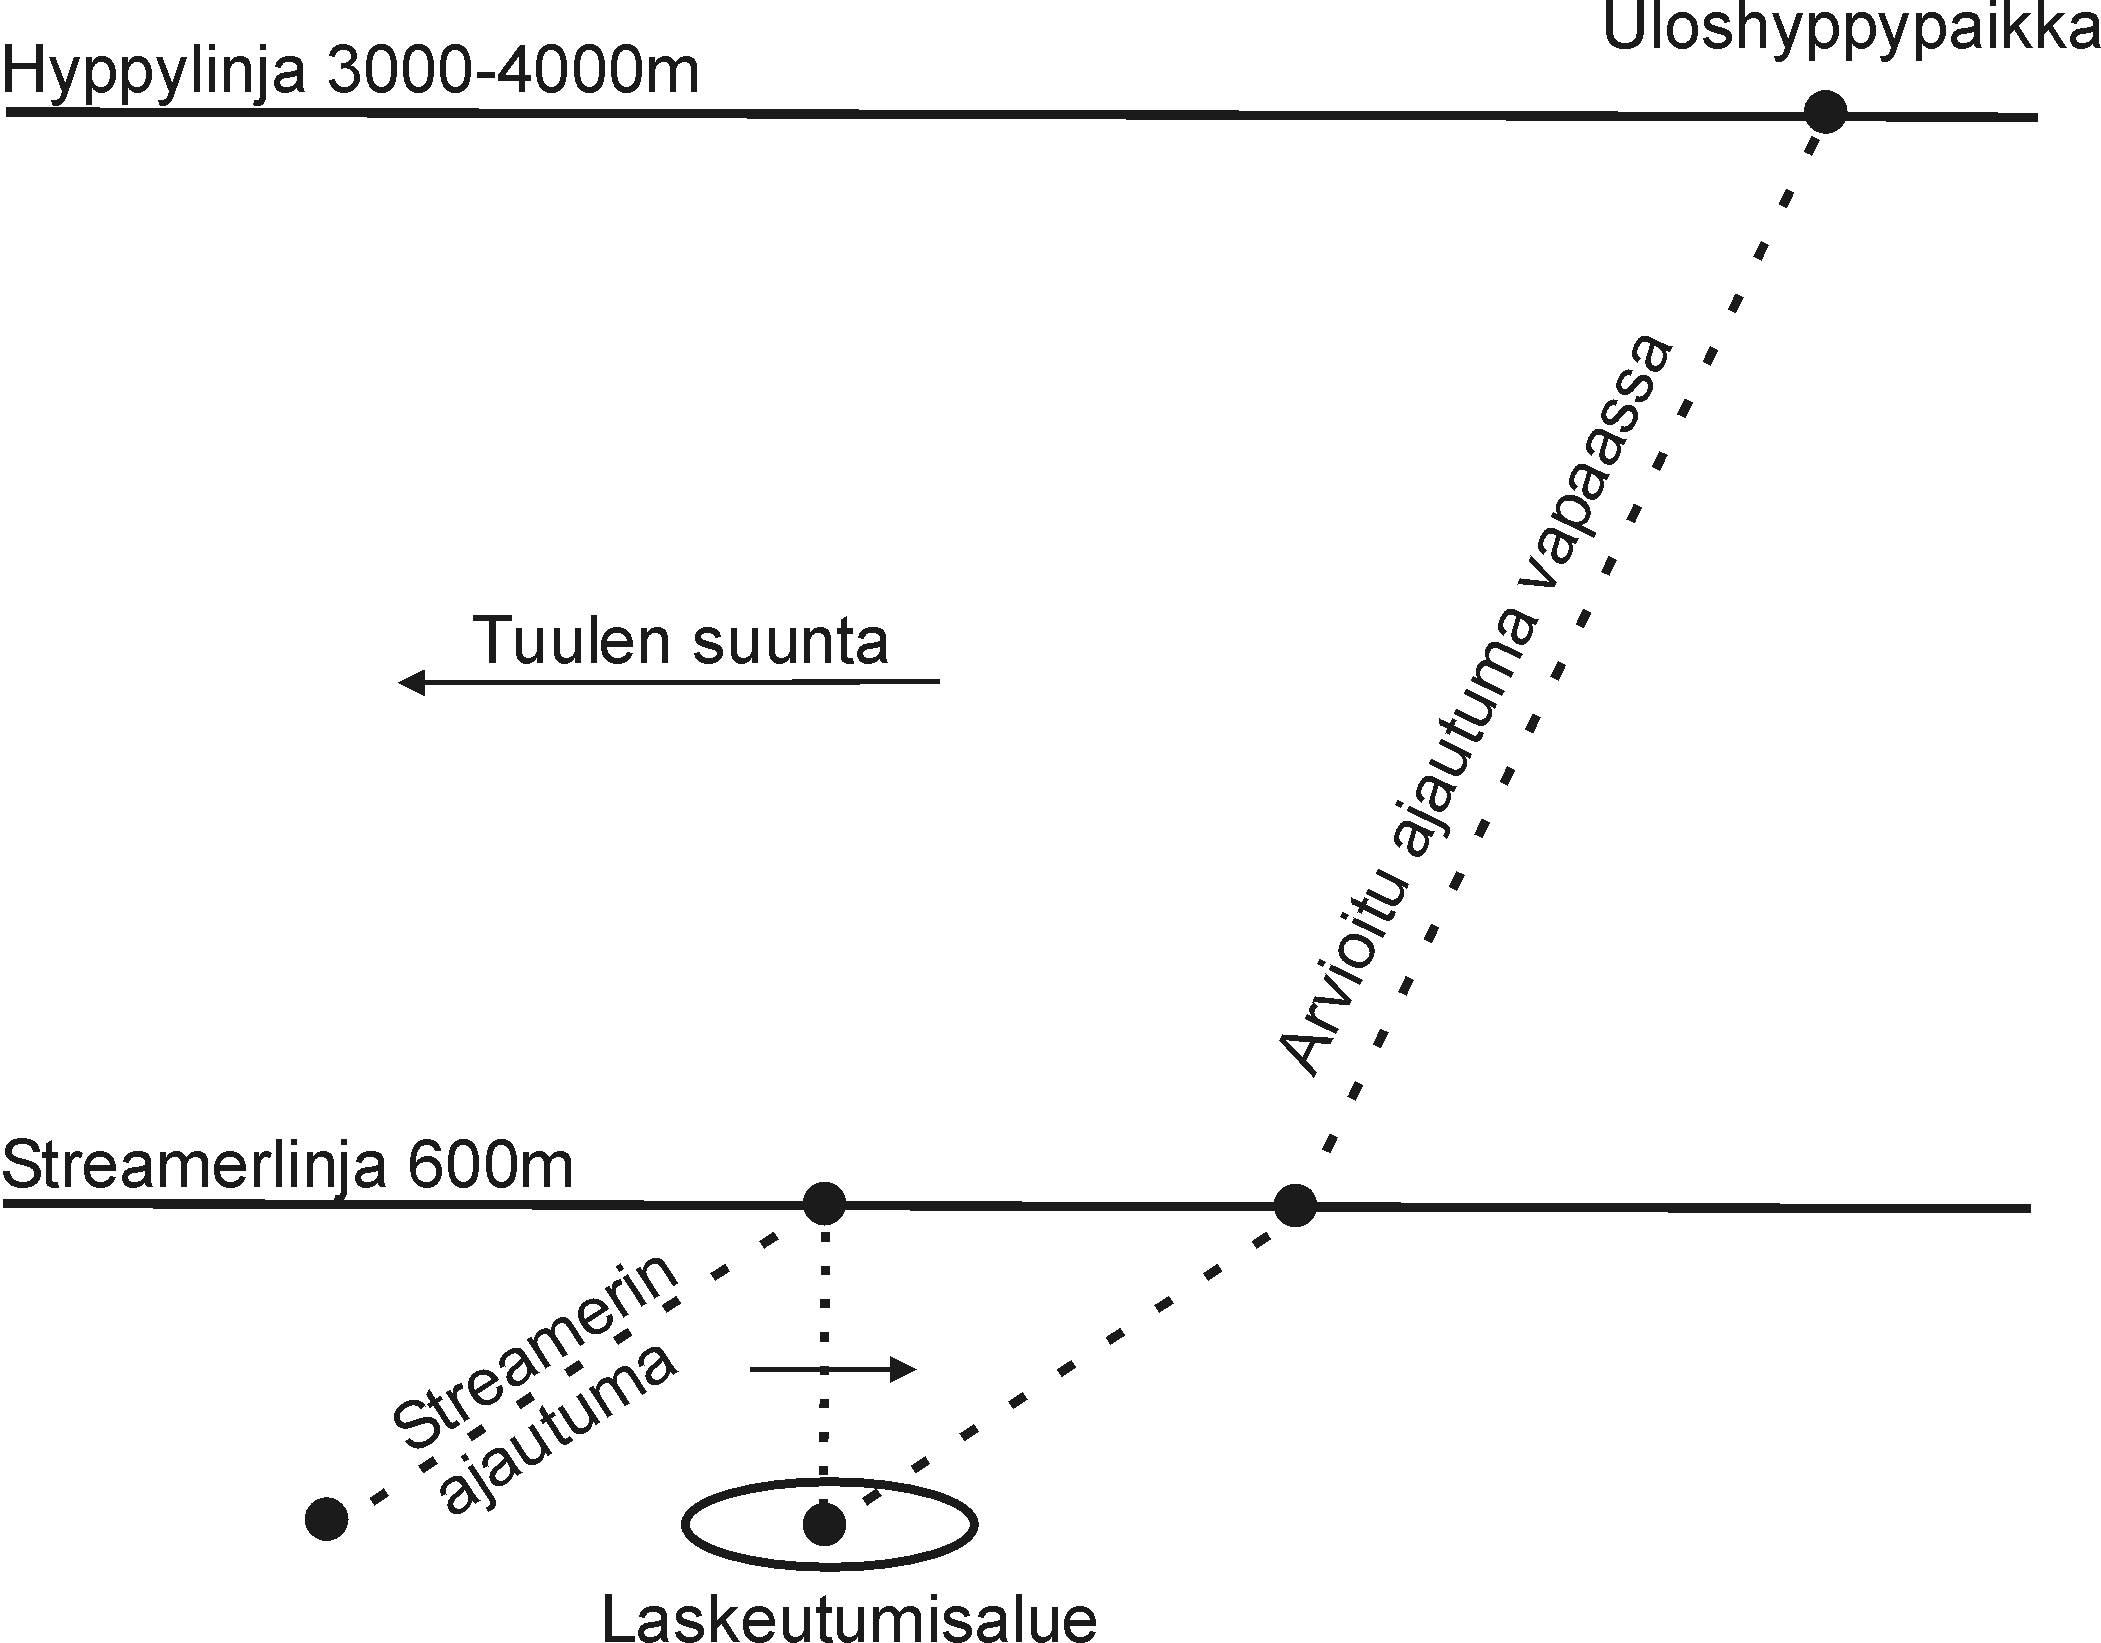
\includegraphics[width=0.99\textwidth]{Paikanmaaritys.jpeg}\captionof{figure}{Uloshyppypaikan määrittäminen korkeammalta hypättäessä}\end{Figure} 

\section{ Linjan määritys }
\label{uloshyppypaikan-maaritys-linjan-maaritys}


Jos lentokoneessa on useampia hyppääjiä/ryhmiä, määritetään hyppylinja huomioiden, että: 

\begin{itemize}
\item  Linja kulkee lasketun UH-paikan läpi. 
\item  Ryhmien välille tulee jäädä turvallinen välimatka. 
\item  Kaikkien tulee päästä turvallisesti laskeutumisalueelle. 
\end{itemize}

Pienillä hyppykoneilla linja ajetaan yleensä vastatuuleen laskeutumisalueen yli. Suurilla hyppykoneilla ajetaan usein sivutuulilinja tai esimerkiksi aina kiitotien suuntainen hyppylinja, jonka etäisyys laskeutumisalueesta riippuu tuuliolosuhteista. Linja voidaan ajaa tarvittaessa myös myötätuuleen. 


Linjan pituudelle ei ole yhtä oikeaa lukua, mutta sitä voidaan arvioida esim. seuraavasti. 

\begin{description}
\item[ ] \hfill \\ 
\textit{Laskuvarjon liitosuhde on välillä 3:1 ja 2:1. Jos hyppääjän varjo on auki 800 metrin korkeudessa ja hyppääjä aloittaa laskeutumiskuvion 300 metrin korkeudessa, hyppääjä voi lentää varjolla arviolta (500 m * 2,5) n. 1300 metrin matkan.}  \hfill \\ 
\end{description}

Tämän varsin konservatiivisen esimerkin mukaan linjan ensimmäinen ryhmä voisi siis poistua koneesta 1300 metriä ennen määritettyä UH-paikkaa ja viimeinen ryhmä 1300 metriä määritetyn pisteen jälkeen. Todellisuudessa linjan pituus voi vaihdella linjan suunnan, laskeutumisalueen, avauskorkeuksien jne. mukaan. Mitä kauempana oikeasta UH-paikasta hypätään, sitä suurempi on riski, että epätarkka tuuliennuste, sääolosuhteiden muutos, matala avaus tai varavarjon käyttö johtaa hyppääjän laskeutumiseen laskeutumisalueen ulkopuolelle. 

\section{Hyppääminen määritetyssä paikassa}
\label{uloshyppypaikan-maaritys-hyppaaminen-maaritetyssa-paikassa}


Lentäjälle annetaan ohjeet suunnitellusta paikasta ja lentosuunnasta ennen koneeseen nousua. Kun kone on saavuttanut hyppykorkeuden, lentäjä ohjaa sovitulle linjalle. Hyppylinja alkaa jo ennen laskeutumisaluetta.  

\subsubsection{Ohjeet lentäjälle}
\label{uloshyppypaikan-maaritys-ohjeet-lentajalle}


Hyppyoven avaamiseen tarvitaan yleensä lupa lentäjältä. Hän antaa avausluvan saatuaan luvan lennonjohdolta tai ilmoitettuaan pudotuksesta lentoliikenteelle. Linjaa korjataan käsimerkein oikealle / vasemmalle / suoraan. Korjaukset voidaan ilmoittaa lentäjälle myös astelukuina (esimerkiksi ''5 VASEMMALLE'') huutamalla tai radiolla (isot hyppykoneet). Tärkeintä on, että korjaukset annetaan rauhallisesti ja varmasti. On huomioitava oma paikka ja näkyvyys, sillä lentäjän voi olla vaikea nähdä hyppääjiä. Turhia korjauksia on vältettävä ja koneen on annettava asettua suoraan ennen seuraavaa tarkastusta.  

\subsubsection{Heitto eteenpäin}
\label{uloshyppypaikan-maaritys-heitto-eteenpain}


Kone heittää hyppääjää lentosuuntaan. Normaalitilanteessa heitto on alle 200 metriä. Erityisen nopeasta koneesta se voi olla suurempi. 

\subsubsection{Paikan katsominen}
\label{uloshyppypaikan-maaritys-paikan-katsominen}


Paikkaa katsottaessa pää työnnetään ulos koneesta ja katsotaan suoraan alaspäin.  


Koneen lentoasento voi aiheuttaa paikan katsomisessa seuraavat virheet: 

\begin{itemize}
\item  Nousussa katsotaan liikaa eteenpäin. 
\item  Laskussa katsotaan liikaa taaksepäin. 
\item  Kallellaan katsotaan liikaa sivulle. 
\end{itemize}

Koneen ollessa vaakalennossa siipi ja horisontti ovat samassa linjassa. 


Lisäksi hyppääjä voi tehdä seuraavia virheitä: 

\begin{itemize}
\item  Katsominen koneen sisältä, jolloin katsotaan liikaa sivulle. 
\item  Katsominen eteenpäin ennakoi uloshyppyä liikaa. 
\end{itemize}
\subsubsection{Ennen uloshyppyä ja uloshyppy}
\label{uloshyppypaikan-maaritys-ennen-uloshyppya-ja-uloshyppy}


Ennen uloshyppypäätöstä hyppääjän on varmistuttava myös ilmatilan vapaudesta. Alla olevia koneita ja hyppääjiä on väistettävä, ja risteävät lentolinjat on myös huomioitava. On huomioitava myös ryhmäuloshypyn vaatima aika, ja varmistettava, että hyppyovi pysyy auki koko uloshypyn ajan ja että ovella ei ole mitään takertumisen mahdollistavia esteitä, esimerkiksi turvavöitä.  


Hyppääjien/ryhmien välillä on oltava riittävät tauot. Vaakaetäisyyttä tulisi yksittäisien hyppääjien välillä olla vähintään 300 metriä, pienillä ryhmillä 500 metriä ja isommilla ryhmillä vielä enemmän. 8–10 sekuntia uloshyppyjen välillä on yleensä hyvä arvio. Tämä riippuu koneen maanopeudesta, joka muuttuu vallitsevien tuuliolosuhteiden mukaan.  


Lentokoneen saaminen tyhjäksi yhdellä linjalla on taloudellisesti järkevää, mutta mitä kauempana määritetystä UH-paikasta hypätään, sitä suuremmaksi tulee riski laskeutua ulos. Päätöksenteko uuden hyppylinjan ottamiseksi voi olla vaikeaa, mutta huono linja vaarantaa muidenkin ilmailijoiden turvallisuuden. 


Varusteet on aina tarkastettava ennen uloshyppyä. 

\section{ Uloshyppyjärjestys }
\label{uloshyppypaikan-maaritys-uloshyppyjarjestys}


Ennen koneeseen nousemista tulee pokalle määrittää uloshyppyjärjestys ja koneeseen noustaan yleensä käänteisessä järjestyksessä. Ylätuulet vaikuttavat pidempään hitaammin putoaviin hyppääjiin sekä ryhmiin ja näin nämä ajautuvat vapaapudotuksessa enemmän kuin nopeammin putoavat hyppääjät sekä ryhmät. Suuremmat muodostelmat putoavat hitaammin kuin pienet muodostelmat ja yksittäiset hyppääjät. Uloshyppyjärjestykseen vaikuttaa siten myös ryhmän koko. Hitaammin putoavat hyppääjät ja ryhmät hyppäävät ennen nopeammin putoavia hyppääjiä ja ryhmiä. Oikealla uloshyppyjärjestyksellä saadaan lisää etäisyyttä hyppääjien ja ryhmien välille ennen purkukorkeutta ja avauksia. 


Uloshyppyjärjestys on yleensä seuraava: 

\begin{itemize}
\item  Isot FS-muodostelmat 
\item  Pienet FS-muodostelmat 
\item  Yksittäiset mahallaan hyppääjät 
\item  Isot free-muodostelmat 
\item  Pienet free-muodostelmat 
\item  Yksittäiset free-hyppääjät 
\item  Tandemit 
\item  Liukuhyppääjät 
\item  Liitopukuhyppääjät 
\end{itemize}

Uloshyppyjärjestykseen vaikuttaa myös avauskorkeus. Normaalia korkeammalla avaavat hyppääjät hyppäävät linjan viimeisinä ennen liitopukuhyppääjiä. Pokan suunnittelussa onkin huomioitava esimerkiksi kupumuodostelma- ja liitopukuhyppääjät siten, etteivät he aiheuta vaaraa muille. 

\section{ Streamer }
\label{uloshyppypaikan-maaritys-streamer}


Ajautuminen varjon varassa voidaan myös arvioida käyttämällä lentokoneesta pudotettavaa streameria. Väriltään streamerin tulee olla maastoon ja vuodenaikaan soveltuva: valkoinen tai keltainen kesällä ja oranssi tai neonvärinen talvella. Kaksivärinen on aina yksiväristä parempi. Streamerin mitat riippuvat käytetyistä materiaaleista, mutta paino-pituussuhteen on oltava sellainen, että streamer putoaa 2 minuuttia 600 metristä. Painoksi käy esimerkiksi metallijauhe, hiekka tai paperi. Alle 5 metriä pitkä streamer on vaikea havaita koneesta.  


Streamerin heittoon on aina saatava lupa lentäjältä/lennonjohdolta ja se heitetään laskeutumisalueen päällä 600 metrin korkeudesta. Streamer voidaan heittää myös oletetusta uloshyppypaikasta tai muusta selkeästä kiintopisteestä. Se on nähtävä koko ajan, joten koneen kaarron on oltava vakio tai lentäjää on ohjeistettava käsimerkein. Aurinko ja heijastumat esimerkiksi vedenpinnasta vaikeuttavat streamerin seurantaa. Streamerin seuraamisen aikana heittäjää ei saa häiritä. Kellotus on tehtävä, ellei streamer ole vakiokokoinen. Streamerin kadotessa heitetään uusi tai kysytään maahenkilöltä havainto sen putoamispaikasta.  

\subsection{ Harjoitus }
\label{uloshyppypaikan-maaritys-harjoitus}

\begin{enumerate}[label=\bfseries \arabic*)]
\item  Harjoitellaan uloshyppypaikan määrittämistä tuulitietojen perusteella. 
\item  Harjoitellaan lentäjän ohjeistamista päivän ensimmäiselle pokalle. 
\item  Harjoitellaan linjan ajoa ja uloshyppypaikan katsomista. 
\end{enumerate}
\end{multicols}

\chapter{Varusteiden tarkastus}
\label{varusteiden-tarkastus}
\thispagestyle{headings}
\begin{multicols}{2}

Laskuvarjohyppääjän varusteet on tarkastettava aina ennen hypylle lähtöä ja uloshyppyä. Oppilaiden varusteet tarkastaa kouluttaja maassa ja koneessa sillä poikkeuksella, että kouluttaja tarkastaa jatkokoulutuksessa olevan oppilaan varusteet ennen koneeseen nousua, mutta oppilas itse vastaa varusteidensa kunnosta ja tarkastuksesta koneessa ennen uloshyppyä. Jatkokoulutuksessa olevat oppilaat ja itsenäiset hyppääjät ovat velvollisia tarkastamaan toistensa varusteet aina ennen uloshyppyä. Varusteiden tarkastamisesta alkaa varsinainen hyppysuoritus ja se päättyy maassa suoritettavaan arviointiin. 


Lainavarusteilla hyppäämisessä on aina riskinsä. Hyppääjä ei pysty oppimaan kaikkia eri avausjärjestelmiä automaatiotasolle, vaan joutuu joka kerta varusteiden muuttuessa keskittymään erityisesti avaustoimenpiteisiin. Näin lainavarusteilla hyppäävän suoritustaso laskee hypyn muulta osalta. Lainavarusteilla hypättäessä tulee aina harjoitella huolellisesti uuden varusteen käyttöä, esimerkiksi apuvarjon tasku voi olla lainavarjossa tiukempi kuin omassa. Huono valmistautuminen lainavarusteen käyttöön on ollut myötävaikuttava tekijä osassa onnettomuuksia. Omat hyppyvarusteet luovat varmuutta hypyille. Lisäksi niistä huolehtiminen on helpompaa ja niiden kunto tiedetään aina. Koneessa on syytä tarkkailla myös muiden hyppääjien hyppyvarusteita. Ajoissa havaittu epäkohta voi estää vaaratilanteen syntymisen. Varusteet tarkistetaan kolme kertaa ennen uloshyppyä. 

\section{ Varusteiden valinta }
\label{varusteiden-tarkastus-varusteiden-valinta}


Varusteet jokainen hyppääjä valitsee itse painonsa, kokemuksensa sekä kouluttajan ohjeet huomioon ottaen. Varusteita valittaessa on huomioitava seuraavaa: 

\begin{itemize}
\item  Henkilökohtaisen vaatetuksen on oltava vuodenaikaan ja säähän sovelias. Hyppyvaatteiden on oltava lämpimiä, mutta samalla myös joustavia. Turha ja liika vaatetus vaikeuttaa suoritusta sekä jäykistää ja hiostuttaa. 
\item  Varjokokonaisuuden ja automaattilaukaisimen asiakirjat on tarkastettava. Pakkausten on oltava alle 12 kk ikäiset ja määräaikaistarkastusten on oltava voimassa. Oppilaspäävarjo sekä varavarjo ja reppu-valjasyhdistelmä tarkastetaan vuoden välein. Automaattilaukaisimet tarkastetaan ja huolletaan 1–4 vuoden välein laitteesta riippuen. 
\item  Varusteet ovat ulkoisesti ehjät ja siistit. Varavarjon vaijerista ja irtipäästökaapeleista tarkastetaan myös niiden vapaa kulku suojaputkissa. 
\item  Automaattilaukaisin säädetään tai se käynnistetään. 
\item  Muista hypyllä tarvittavista varusteista tarkastetaan korkeusmittarin, kypärän, suojalasien, koukkupuukon, haalarin, sormikkaiden, kenkien ja pelastusliivien(tarvittaessa) kunto, toimivuus ja soveltuvuus laskuvarjohyppykäyttöön. Varusteissa ei saa olla ulokkeita tai osia, jotka voivat tarttua kiinni. 
\item  Varusteet ovat sopivat ja säädöt kunnossa. Tarvittaessa valjaiden pituussäätöä muutetaan ja haalari jne. vaihdetaan sopivampiin huomioiden hyppysuoritus ja sääolosuhteet. 
\end{itemize}

Tarkastukseen on varattava riittävästi aikaa, sillä kiireessä valitut ja sovitetut varusteet voivat aiheuttaa hypyllä ongelmia. Esimerkiksi itseaukaisukahva ei ole muuttuneista valjassäädöistä johtuen totutulla paikalla tai hyppylasit jäävät löysälle ja tippuvat. Huolellinen ensimmäinen tarkastusvaihe nopeuttaa muita vaiheita. 

\section{ Maassa ennen koneen lastaamista }
\label{varusteiden-tarkastus-maassa-ennen-koneen-lastaamista}


Varusteiden toinen tarkastusvaihe suoritetaan, kun varusteet on puettu päälle. Tarkastus tehdään ennen koneeseen nousua. Varusteiden tarkastuksessa noudatetaan aina samaa, seuraavassa lueteltua mallia: 

\begin{itemize}
\item  Varusteet on puettu oikein. 
\item  Kaikki hypyllä tarvittavat varusteet ovat mukana oikeilla paikoillaan. Korkeusmittari on näkyvissä ja nollattu sekä koukkupuukko on saatavilla. Kahvat ovat omilla paikoillaan ja ne näkyvät. 
\item  Kaikki lukot, soljet ja hihnat ovat kiinni. Hihnojen päät on työnnetty valjaskumilenkkien alta hihnataskuihin. 
\item  Automaattilaukaisin on päällä ja se on oikein säädetty. 
\item  Hyppykaveri tarkastaa takaa, että pää- ja varavarjon läpät ovat kiinni. Pinnitarkastus suoritetaan, jos läppä tai läpät ovat auenneet I vaiheen jälkeen varusteita päälle puettaessa. 
\end{itemize}

Yleisimmät virheet varusteiden pukemisessa löytyvät hihnoista. Ne ovat joko kierteellä, löysinä tai niiden päät eivät ole valjaskumilenkkien alla. Myös mittarin asetus on voinut muuttua ja repun läpät aueta, jos varusteet päälle puettuna on liikuttu varomattomasti. Kypärä, suojalasit tai sormikkaat unohtuvat helposti, ellei niitä varata ja pueta päälle ennen tätä tarkastusvaihetta. 

\section{ Ennen uloshyppyä }
\label{varusteiden-tarkastus-ennen-uloshyppya}


Tarkastus ennen uloshyppyä aloittaa varsinaisen hyppysuorituksen. Tarkastus aloitetaan 100–300 metriä ennen uloshyppykorkeutta. Tarkastuksessa noudatetaan samaa periaatetta kuin edellisessäkin vaiheessa. Tarkastus on silmämääräinen ja siinä tehdään vain tarvittavat muutokset ja kiristykset. Liikkuminen koneessa ja uloshyppy on aina suoritettava varoen ja varusteita suojaten. Tässä vaiheessa tarkastetaan seuraavat asiat: 

\begin{itemize}
\item  Kypärä ja sormikkaat ovat puettuna päälle ja hyppylasit kiristettyinä hyppykireyteen. 
\item  Varavarjon pakkolaukaisuhihnan lukko on kiinni ja paikoillaan. 
\item  Korkeusmittari näyttää oikein ja on luettavissa. Automaattilaukaisin FXC-12000 on JUMP-asennossa. 
\item  Irtipäästöpampula, varavarjonkahva ja päävarjon avauskahva ovat paikallaan sekä näkyvissä (pois lukien BOC eli repun pohjassa sijaitseva avauskahva, jonka pitää olla esteettömästi saatavilla, tarkista sijainti koskettamalla BOC-avauskahvaa). 
\item  Rinta- ja reisihihnat ovat kireällä ja mahdolliset lukot ovat kiinni. 
\item  Hyppykaveri tarkastaa takaa, että pää- ja varavarjon läpät ovat kiinni. Pinnitarkastus suoritetaan, jos läppä tai läpät ovat auenneet. Tarraläpän alla oleva pinni on hyvä tarkastaa aina. 
\end{itemize}

Varusteiden tarkastus ennen uloshyppyä voi huolimattomasti suunnitellulla hypyllä jäädä kokonaan tekemättä. Rutiinista poikkeaminen luo hypylle epävarman tunteen, joka aiheuttaa usein hyppysuorituksen epäonnistumisen. Varjon avautuminen koneessa aiheutuu yleensä turhasta ja huolimattomasta liikkumisesta tai huonokuntoisesta luupista. Hyppyovea ei saa koskaan avata, jos koneessa on varjo auki, vaan kaikki tulevat silloin koneella alas. Varusteiden itsenäinen tarkastus vaaditaan jokaisella hypyllä tämän koulutuksen jälkeen. Kouluttaja vastaa edelleen oppilaasta koko jatkokoulutuksen ajan. 

\section{Harjoitus}
\label{varusteiden-tarkastus-harjoitus}

\begin{enumerate}[label=\bfseries \arabic*)]
\item  Suoritetaan tarkastukset opetuksen yhteydessä. 
\item  Tutustutaan koneesta mahdollisesti löytyviin paikkoihin, joihin hyppyvarusteet voivat takertua. 
\end{enumerate}
\end{multicols}

\chapter{NOVA-Peruskoulutuksen suoritukset}
\label{nova-peruskoulutuksen-suoritukset}
\thispagestyle{headings}
\begin{multicols}{2}
\section{ 8'' }
\label{nova-peruskoulutuksen-suoritukset-8}

\subsection{ Oppilaan toiminta }
\label{nova-peruskoulutuksen-suoritukset-oppilaan-toiminta}


Käytä tasokoulutuksessa opittuja asioita: suora uloshyppy, asennon stabilointi uloshypyn jälkeen, korkeuden tarkkailu ja stabiili asento. 

\subsection{ Oppimistavoitteet }
\label{nova-peruskoulutuksen-suoritukset-oppimistavoitteet}

\begin{enumerate}[label=\bfseries \arabic*)]
\item  Stabiili asento 5 sekunnissa 
\item  Avaustoimenpiteet oikeaan aikaan (7-10 s uloshypystä) 
\end{enumerate}
\subsection{ Hyppylennolla }
\label{nova-peruskoulutuksen-suoritukset-hyppylennolla}


Tarkista omat varusteesi, ilmatila, pilvet ja huomioi mahdollinen exit-väli. 

\subsection{ Hypyn kulku }
\label{nova-peruskoulutuksen-suoritukset-hypyn-kulku}

\begin{description}
\item[TAIVUTA] \hfill \\ 
Tee uloshyppy koneesta ottaen välittömästi ilmavirtaan päästyäsi hyvä taivutus.  \hfill \\ 
Rentouta asento uloshypyn jälkeen  \hfill \\ 
Tarkkaile korkeutta  \hfill \\ 
\end{description}
\begin{description}
\item[8-SEKUNTIA ] \hfill \\ 
Aloita avaustoimenpiteet: Näytä avausmerkki.  \hfill \\ 
\end{description}
\begin{description}
\item[TAIVUTA] \hfill \\ 
Varmistetaan taivutus ja asento.  \hfill \\ 
\item[TARTU] \hfill \\ 
Vasen käsi vartalon jatkeeksi ja oikea käsi apuvarjolle, tiukka ote. \hfill \\ 
\end{description}
\begin{description}
\item[VEDÄ] \hfill \\ 
Heitä apuvarjo ilmavirtaan. \hfill \\ 
Palauta perusasento.  \hfill \\ 
\end{description}
\begin{description}
\item[101] \hfill \\ 
Aloitetaan laskeminen alusta vedon jälkeen.  \hfill \\ 
\item[102..104] \hfill \\ 
Varjo avautuu ja tehdään sen lopullinen avaaminen.  \hfill \\ 
\item[105] \hfill \\ 
Vilkaistaan olkapään yli tarvittaessa (turbulenssin poisto). \hfill \\ 
\end{description}

\end{multicols}\pagebreak\begin{multicols}{2} 

\section{ 5'' }
\label{nova-peruskoulutuksen-suoritukset-5}

\subsection{ Oppilaan toiminta }
\label{nova-peruskoulutuksen-suoritukset-oppilaan-toiminta}


Käytä tasokoulutuksessa opittuja asioita: suora uloshyppy, asennon stabilointi uloshypyn jälkeen, korkeuden tarkkailu ja stabiili asento. 

\subsection{ Oppimistavoitteet }
\label{nova-peruskoulutuksen-suoritukset-oppimistavoitteet}

\begin{enumerate}[label=\bfseries \arabic*)]
\item  Avaustoimenpiteet stabiilista asennosta oikeaan aikaan. (4-7 s uloshypystä) 
\end{enumerate}
\subsection{ Hyppylennolla }
\label{nova-peruskoulutuksen-suoritukset-hyppylennolla}


Tarkista omat varusteesi, ilmatila, pilvet ja huomioi mahdollinen exit-väli. 

\subsection{ Hypyn kulku }
\label{nova-peruskoulutuksen-suoritukset-hypyn-kulku}

\begin{description}
\item[TAIVUTA] \hfill \\ 
Tee uloshyppy koneesta ottaen välittömästi ilmavirtaan päästyäsi hyvä taivutus.  \hfill \\ 
Rentouta asento uloshypyn jälkeen  \hfill \\ 
Tarkkaile korkeutta  \hfill \\ 
\end{description}
\begin{description}
\item[5-SEKUNTIA ] \hfill \\ 
Aloita avaustoimenpiteet: Näytä avausmerkki.  \hfill \\ 
\end{description}
\begin{description}
\item[TAIVUTA] \hfill \\ 
Varmistetaan taivutus ja asento.  \hfill \\ 
\item[TARTU] \hfill \\ 
Vasen käsi vartalon jatkeeksi ja oikea käsi apuvarjolle, tiukka ote \hfill \\ 
\end{description}
\begin{description}
\item[VEDÄ] \hfill \\ 
Heitä apuvarjo ilmavirtaan \hfill \\ 
Palauta perusasento.  \hfill \\ 
\end{description}
\begin{description}
\item[101] \hfill \\ 
Aloitetaan laskeminen alusta vedon jälkeen.  \hfill \\ 
\item[102..104] \hfill \\ 
Varjo avautuu ja tehdään sen lopullinen avaaminen.  \hfill \\ 
\item[105] \hfill \\ 
Vilkaistaan olkapään yli tarvittaessa (turbulenssin poisto). \hfill \\ 
\end{description}
\end{multicols}

\chapter{PL-Peruskoulutuksen suoritukset}
\label{pl-peruskoulutuksen-suoritukset}
\thispagestyle{headings}
\begin{multicols}{2}
\section{ 15'' }
\label{pl-peruskoulutuksen-suoritukset-15}


Avaustoimenpiteet aloitetaan 1200 metrin korkeudessa mittarin mukaan. Vapaapudotusaika on noin 15 sekuntia. Lisää tästä lähin avaustoimenpiteisiisi avausmerkki, jolla ilmoitat muille avaavasi varjosi, eli heilauta käsiäsi ristiin pääsi edessä.  

\subsection{ Oppimistavoitteet }
\label{pl-peruskoulutuksen-suoritukset-oppimistavoitteet}

\begin{enumerate}[label=\bfseries \arabic*)]
\item  Stabiili asento  
\item  HD-apuvarjo heitetty oikein ilmavirtaan (jos hypyllä tehdään HD-totuttelu) 
\end{enumerate}
\subsection{ Hyppylennolla }
\label{pl-peruskoulutuksen-suoritukset-hyppylennolla}

\begin{itemize}
\item Kertaa suoritus mielessäsi 
\item Keskity suoritukseesi 
\item 3X3 -tarkastus ennen hyppyä (\ref{laskuvarjokalusto-ja-hyppyvarusteet-3x3-tarkastus} s.\pageref{laskuvarjokalusto-ja-hyppyvarusteet-3x3-tarkastus}) 
\end{itemize}
\subsection{ Hypyn kulku }
\label{pl-peruskoulutuksen-suoritukset-hypyn-kulku}

\begin{description}
\item[TAIVUTA] \hfill \\ 
Tee uloshyppy koneesta ottaen välittömästi ilmavirtaan päästyäsi hyvä taivutus. \hfill \\ 
Rentouta asento uloshypyn jälkeen \hfill \\ 
Tarkkaile korkeutta \hfill \\ 
\item[1200 metriä] \hfill \\ 
Aloita avaustoimenpiteet: Näytä avausmerkki. \hfill \\ 
\item[TAIVUTA ] \hfill \\ 
Varmistetaan taivutus ja asento. \hfill \\ 
\item[TARTU] \hfill \\ 
Vasen käsi kypärän päälle eteen vartalon normaaliksi jatkeeksi ja oikea käsi kahvalle, tiukka ote \hfill \\ 
\item[VEDÄ] \hfill \\ 
	\begin{itemize}
	\item  Veto kahvasta putken tai taskun suuntaan 
	\item  Palauta perusasento. 
	\end{itemize}
\item[101 ] \hfill \\ 
Aloitetaan laskeminen alusta vedon jälkeen. \hfill \\ 
\item[102..104 ] \hfill \\ 
Varjo avautuu ja tehdään sen lopullinen avaaminen. \hfill \\ 
\item[105 ] \hfill \\ 
Vilkaistaan olkapään yli tarvittaessa (turbulenssin poisto). \hfill \\ 
\end{description}

\end{multicols}\pagebreak\begin{multicols}{2} 

\section{ Suora uloshyppy }
\label{pl-peruskoulutuksen-suoritukset-suora-uloshyppy}


Tavoitteena on oppia uloshyppy suorana, eli suoraan koneen sisältä ilmavirtaan. 

\subsubsection{Streeva-kone}
\label{pl-peruskoulutuksen-suoritukset-streeva-kone}

\begin{enumerate}[label=\bfseries \arabic*)]
\item Vasen jalka astinlaudalle. 
\item Kädet oviaukon reunalle. 
\item Kohottaudutaan koneen ulkopuolelle varoen repun osumista koneeseen. 
\item Käännetään rinta koneen etenemissuuntaan. 
\item Ponnistetaan ilmavirran suuntaan taaksepäin. 
\item Taivutus, katse ylös, jalat lähes suorina ja kädet taakse delta-asentoon. 
\item Sitä mukaa kun asento kääntyy vaakatasoon, otetaan perusasento. 
\end{enumerate}
\subsubsection{Muut koneet}
\label{pl-peruskoulutuksen-suoritukset-muut-koneet}

\begin{enumerate}[label=\bfseries \arabic*)]
\item Siirrytään oviaukolle kyykkyyn tai seisaalleen, varoen repun osumista koneeseen. 
\item Ponnistetaan ilmavirran suuntaan eteenpäin, rinta koneen etenemissuuntaan. 
\item Taivutus, jalat lähes suorina ja kädet taakse delta-asentoon. 
\item Sitä mukaa kun asento kääntyy vaakatasoon, otetaan perusasento. 
\end{enumerate}
\subsection{ Oppimistavoitteet }
\label{pl-peruskoulutuksen-suoritukset-oppimistavoitteet}

\begin{enumerate}[label=\bfseries \arabic*)]
\item  Stabiili asento 5 sekunnin kuluessa 
\item  Suunnan hallinta, ei tahatonta yli 360° käännöstä. 
\end{enumerate}
\subsection{ Hyppylennolla }
\label{pl-peruskoulutuksen-suoritukset-hyppylennolla}

\begin{itemize}
\item Kertaa suoritus mielessäsi 
\item Keskity suoritukseesi 
\item 3X3 -tarkastus ennen hyppyä (\ref{laskuvarjokalusto-ja-hyppyvarusteet-3x3-tarkastus} s.\pageref{laskuvarjokalusto-ja-hyppyvarusteet-3x3-tarkastus}) 
\end{itemize}
\subsection{ Hypyn kulku }
\label{pl-peruskoulutuksen-suoritukset-hypyn-kulku}

\begin{description}
\item[TAIVUTA] \hfill \\ 
Tee uloshyppy koneesta ottaen välittömästi ilmavirtaan päästyäsi hyvä delta-asento. \hfill \\ 
Asennon käännyttyä vaakatasoon (tyypillisesti noin 5 sekunnin jälkeen) ota perusasento \hfill \\ 
Tarkkaile korkeutta \hfill \\ 
\item[1200 metriä] \hfill \\ 
Aloita avaustoimenpiteet. \hfill \\ 
\end{description}

\end{multicols}\pagebreak\begin{multicols}{2} 

\section{ Sukellusuloshyppy }
\label{pl-peruskoulutuksen-suoritukset-sukellusuloshyppy}


Koneesta sukelletaan ulos ja pidetään suunta. 

\subsubsection{Streeva-kone}
\label{pl-peruskoulutuksen-suoritukset-streeva-kone}

\begin{enumerate}[label=\bfseries \arabic*)]
\item Oikea jalka astimelle, varpaat peräsimen suuntaan. 
\item Kädet oviaukon reunalle. 
\item Kohottaudutaan koneen ulkopuolelle varoen repun osumista koneeseen. 
\item Käännytään koneen peräsintä kohti. 
\item Sukelletaan ilmavirran suuntaan taaksepäin, rinta ilmavirtaan. 
\item Taivutus, jalat koukkuun ja kädet eteen leveälle. 
\item Sitä mukaa kun asento kääntyy vaakatasoon, otetaan perusasento. 
\end{enumerate}
\subsubsection{Muut koneet}
\label{pl-peruskoulutuksen-suoritukset-muut-koneet}

\begin{enumerate}[label=\bfseries \arabic*)]
\item Siirrytään oviaukolle kyykkyyn tai seisaalleen, varoen repun osumista koneeseen. 
\item Sukelletaan ilmavirran suuntaan taaksepäin, rinta ilmavirtaan. 
\item Taivutus, jalat koukkuun ja kädet eteen leveälle. 
\item Sitä mukaa kun asento kääntyy vaakatasoon, otetaan perusasento. 
\end{enumerate}
\subsection{ Oppimistavoitteet }
\label{pl-peruskoulutuksen-suoritukset-oppimistavoitteet}

\begin{enumerate}[label=\bfseries \arabic*)]
\item  Stabiili asento 5 sekunnin kuluessa 
\item  Suunnan hallinta, ei tahatonta yli 360° käännöstä. 
\end{enumerate}
\subsection{ Hyppylennolla }
\label{pl-peruskoulutuksen-suoritukset-hyppylennolla}

\begin{itemize}
\item Kertaa suoritus mielessäsi 
\item Keskity suoritukseesi 
\item 3X3 -tarkastus ennen hyppyä (\ref{laskuvarjokalusto-ja-hyppyvarusteet-3x3-tarkastus} s.\pageref{laskuvarjokalusto-ja-hyppyvarusteet-3x3-tarkastus}) 
\end{itemize}
\subsection{ Hypyn kulku }
\label{pl-peruskoulutuksen-suoritukset-hypyn-kulku}

\begin{description}
\item[TAIVUTA] \hfill \\ 
Tee sukellus-uloshyppy \hfill \\ 
Pidä asentosi symmetrisenä, jalat koukussa \hfill \\ 
Asennon käännyttyä vaakatasoon (tyypillisesti noin 5 sekunnin jälkeen) ota perusasento \hfill \\ 
Tarkkaile korkeutta \hfill \\ 
\item[1200 metriä] \hfill \\ 
Aloita avaustoimenpiteet. \hfill \\ 
\end{description}

\end{multicols}\pagebreak\begin{multicols}{2} 

\section{ 360° käännökset }
\label{pl-peruskoulutuksen-suoritukset-360deg-kaannokset}


Uloshypyn jälkeen tehdään hallittu 360 asteen käännös. 

\begin{enumerate}[label=\bfseries \arabic*)]
\item Otetaan kiintopiste horisontista. 
\item Painetaan hartialinja alas halutun käännöksen suuntaan. 
\item Otetaan perusasento ennen kiintopistettä. 
\item Vähän ennen kiintopistettä tehdään pieni vastaliike, jotta käännös pysähtyy täsmällisesti. 
\end{enumerate}

Pidä taivutus koko käännöksen ajan. Tarkkaile korkeutta. 

\subsection{ Oppimistavoitteet }
\label{pl-peruskoulutuksen-suoritukset-oppimistavoitteet}

\begin{enumerate}[label=\bfseries \arabic*)]
\item  360° käännös sovittuun suuntaan ja hallittu pysäytys. 
\item  Asento säilyy stabiilina. 
\end{enumerate}
\subsection{ Hyppylennolla }
\label{pl-peruskoulutuksen-suoritukset-hyppylennolla}

\begin{itemize}
\item Kertaa suoritus mielessäsi 
\item Keskity suoritukseesi 
\item 3X3 -tarkastus ennen hyppyä 
\end{itemize}
\subsection{ Hypyn kulku }
\label{pl-peruskoulutuksen-suoritukset-hypyn-kulku}

\begin{description}
\item[TAIVUTA] \hfill \\ 
Tee uloshyppy koneesta \hfill \\ 
Asennon käännyttyä vaakatasoon (tyypillisesti noin 5 sekunnin jälkeen) ota perusasento \hfill \\ 
Ota kiintopiste maasta/horisontista ja tee 360° käännös sovittuun suuntaan \hfill \\ 
Tarkkaile korkeutta, toista harjoitus jos korkeutta on riittävästi. \hfill \\ 
\item[1600 metriä] \hfill \\ 
Lopeta työskentely ja valmistaudu päävarjon avaamiseen. \hfill \\ 
\item[1200 metriä] \hfill \\ 
Aloita avaustoimenpiteet. \hfill \\ 
\end{description}

\end{multicols}\pagebreak\begin{multicols}{2} 

\section{ Tynnyri ja takavoltti }
\label{pl-peruskoulutuksen-suoritukset-tynnyri-ja-takavoltti}

\subsubsection{ Tynnyri }
\label{pl-peruskoulutuksen-suoritukset-tynnyri}


Tynnyri on freeasentojen perusliike, sillä isommilla freekuvilla purun jälkeen liu’uttaessa voidaan tekemällä liu’usta tynnyri tarkastaa vapaa ilmatila ennen avausta. Tynnyrissä on tarkoitus kääntyä vatsaltaan kyljen kautta täysi vaakakierre. 


Tynnyri tehdään seuraavasti: 

\begin{enumerate}[label=\bfseries \arabic*)]
\item Otetaan perusasento. 
\item Viedään toinen käsi vartalon lähelle tai alle. 
\item Kierretään vartaloa siten, että lähelle tuodun käden puolta painetaan alaspäin. 
\item Asennon käännyttyä selälleen jatketaan liikettä vielä toisen kyljen ympäri. 
\item Palautetaan perusasento. 
\end{enumerate}
\subsubsection{ Takavoltti }
\label{pl-peruskoulutuksen-suoritukset-takavoltti}


Takavoltissa tehdään voltti vaaka-akselin ympäri taaksepäin. 


Takavoltti tehdään seuraavasti: 

\begin{enumerate}[label=\bfseries \arabic*)]
\item Otetaan perusasento. 
\item Vedetään jalat nopeasti yhteen koukkuun. 
\item Painetaan käsillä alaspäin ilmavirtaa vasten. 
\item Pään ollessa alaspäin palautetaan perusasento. 
\end{enumerate}

Kädet pidetään perusasennossa suorina, hieman sivuille käännettyinä. Jalat laitetaan yhteen ja koukkuun vartalon alle. Painetaan käsillä alaspäin ilmavirtaa vasten. Pysäytys tapahtuu palauttamalla perusasento. Jalkojen nopea ja yhtaikainen tuonti vartalon alle takaa voltin onnistumisen. Käsillä autetaan ympäri menoa ja estetään asennon kallistuminen sivulle. 

\subsection{ Oppimistavoitteet }
\label{pl-peruskoulutuksen-suoritukset-oppimistavoitteet}

\begin{itemize}
\item  Asento saadaan hallintaan liikkeiden jälkeen. 
\end{itemize}
\subsection{ Hyppylennolla }
\label{pl-peruskoulutuksen-suoritukset-hyppylennolla}

\begin{itemize}
\item Kertaa suoritus mielessäsi. 
\item Keskity suoritukseesi. 
\item 3X3 -tarkastus ennen hyppyä. 
\end{itemize}
\subsection{ Hypyn kulku }
\label{pl-peruskoulutuksen-suoritukset-hypyn-kulku}

\begin{description}
\item[TAIVUTA] \hfill \\ 
Tee uloshyppy koneesta \hfill \\ 
Asennon käännyttyä vaakatasoon (tyypillisesti noin 5 sekunnin jälkeen) ota perusasento \hfill \\ 
Tee tynnyri \hfill \\ 
Tarkkaile korkeutta \hfill \\ 
Tee takavoltti \hfill \\ 
Tarkkaile korkeutta \hfill \\ 
Mikäli korkeutta on vielä yli 1800 metriä, toista harjoitus. \hfill \\ 
\item[1800 metriä] \hfill \\ 
Lopeta työskentely ja valmistaudu päävarjon avaamiseen. \hfill \\ 
\item[1200 metriä] \hfill \\ 
Aloita avaustoimenpiteet. \hfill \\ 
\end{description}

\end{multicols}\pagebreak\begin{multicols}{2} 

\end{multicols}

\chapter{Peruskoulutuksen muut suoritukset}
\label{peruskoulutuksen-muut-suoritukset}
\thispagestyle{headings}
\begin{multicols}{2}
\section{ Selkälento }
\label{peruskoulutuksen-muut-suoritukset-selkalento}


Selkälennossa rintahihnassa oleva korkeusmittari ei välttämättä näytä oikein. 

\subsection{ Oppilaan toiminta }
\label{peruskoulutuksen-muut-suoritukset-oppilaan-toiminta}

\begin{itemize}
\item Harjoittele suorituksen vaiheet: 
	\begin{enumerate}[label=\bfseries \arabic*)]
	\item  Käännetään asento kyljelleen käyttämällä kättä vartalossa 
	\item  Taivutetaan samalla asento väärinpäin, istuma-asentoon, jalat koukistettuina 
	\item  Lennetään muutama sekunti selällään (huomioidaan korkeus) 
	\item  Käännetään asento perusasentoon taivuttamalla 
	\end{enumerate}
\end{itemize}
\subsection{ Oppimistavoitteet }
\label{peruskoulutuksen-muut-suoritukset-oppimistavoitteet}

\begin{enumerate}[label=\bfseries \arabic*)]
\item  Pääsy perusasennosta selkälentoon 
\item  Asennon hallinta selällään (pieni kääntyminen ok, lattakierre ei) 
\end{enumerate}
\subsection{ Hyppylennolla }
\label{peruskoulutuksen-muut-suoritukset-hyppylennolla}

\begin{itemize}
\item Kertaa suoritus mielessäsi 
\item Keskity suoritukseesi 
\item 3X3 -tarkastus ennen hyppyä 
\end{itemize}
\subsection{ Hypyn kulku }
\label{peruskoulutuksen-muut-suoritukset-hypyn-kulku}

\begin{description}
\item[TAIVUTA] \hfill \\ 
Tee uloshyppy koneesta ottaen välittömästi ilmavirtaan päästyäsi hyvä taivutus. \hfill \\ 
Rentouta asento uloshypyn jälkeen \hfill \\ 
Ota ensin perusasento ja käänny tämän jälkeen selälleen \hfill \\ 
Tarkkaile korkeutta \hfill \\ 
Muutaman sekunnin jälkeen käännä asento takaisin mahalleen perusasentoon \hfill \\ 
Mikäli korkeutta on vielä yli 1800 metriä, toista harjoitus. \hfill \\ 
\item[1800 metriä] \hfill \\ 
Lopeta työskentely ja valmistaudu päävarjon avaamiseen.  \hfill \\ 
\item[1200 metriä] \hfill \\ 
Aloita avaustoimenpiteet. \hfill \\ 
\end{description}

\end{multicols}\pagebreak\begin{multicols}{2} 

\section{ Liuku }
\label{peruskoulutuksen-muut-suoritukset-liuku}


Liu’un tavoitteena on liikkua vaakatasossa mahdollisimman kauaksi muihin hyppääjiin nähden samalla, kun pudotaan alaspäin. Liuku ei ole siis syöksyä tai tikkaamista. Putoamisnopeus voi kasvaa liu’un aikana. Korkeuden tarkkailu on tärkeää, sillä liu’un pysäytys vaatii myös aikansa. Varjon avaamista suoraan liu’usta ei suositella. Hyvä liuku on ensiarvoisen tärkeä taito laskuvarjohyppääjällä, sillä ainoastaan hyvällä liu’ulla pystyy varmistamaan riittävän välimatkan muihin hyppääjiin purun jälkeen. 


Liuku tehdään seuraavasti: 

\begin{enumerate}[label=\bfseries \arabic*)]
\item Otetaan kiintopiste edestä, maasta. 
\item Oikaistaan jalat nilkkoja myöten. 
\item Viedään kädet sivuille taakse, lähelle vartaloa. 
\item Painetaan olkapäät alas eteen. 
\item Ohjataan liukusuuntaa kämmenillä. 
\item Tarkkaillaan korkeutta, muita hyppääjiä sekä liu'utaan kohti kiintopistettä. 
\item Palautetaan perusasento rauhallisesti ottamalla ensin taivutus ja sen jälkeen kädet ja jalat perusasentoon 
\end{enumerate}
\subsection{ Oppilaan toiminta }
\label{peruskoulutuksen-muut-suoritukset-oppilaan-toiminta}

\begin{itemize}
\item  Ota selvää hyppylinjan suunnasta, jotta osaat valita oikean liukusuunnan (poispäin linjasta). 
\end{itemize}
\subsection{ Oppimistavoitteet }
\label{peruskoulutuksen-muut-suoritukset-oppimistavoitteet}

\begin{enumerate}[label=\bfseries \arabic*)]
\item  Liu'u sovittuun suuntaan ja pysy suunnassa 
\item  Liuku liikkuu eteenpäin 
\item  Liuku ei nyöki 
\end{enumerate}
\subsection{ Hyppylennolla }
\label{peruskoulutuksen-muut-suoritukset-hyppylennolla}

\begin{itemize}
\item Kertaa suoritus mielessäsi 
\item Keskity suoritukseesi 
\item 3X3 -tarkastus ennen hyppyä 
\end{itemize}
\subsection{ Hypyn kulku }
\label{peruskoulutuksen-muut-suoritukset-hypyn-kulku}

\begin{description}
\item[TAIVUTA] \hfill \\ 
Tee uloshyppy koneesta ottaen välittömästi ilmavirtaan päästyäsi hyvä taivutus. \hfill \\ 
Rentouta asento uloshypyn jälkeen \hfill \\ 
Käänny liukusuuntaan, ota liukuasento ja liu'u noin 5 sekuntia \hfill \\ 
Pysäytä liuku \hfill \\ 
Tarkkaile korkeutta \hfill \\ 
Mikäli korkeutta on vielä jäljellä, käänny 180° ja toista liuku. \hfill \\ 
\item[1600 metriä] \hfill \\ 
Lopeta työskentely ja valmistaudu päävarjon avaamiseen.  \hfill \\ 
\item[1200 metriä] \hfill \\ 
Aloita avaustoimenpiteet. \hfill \\ 
\end{description}

\end{multicols}\pagebreak\begin{multicols}{2} 

\section{ FS-liuku }
\label{peruskoulutuksen-muut-suoritukset-fs-liuku}


FS-liuku on liikesarja, joka suoritetaan jokaisen FS-hypyn lopuksi. Liikesarjassa annettavilla merkeillä viestitään kanssahyppääjille niitä toimenpiteitä, mitä on aikomus seuraavaksi tehdä. 

\subsection{ Oppilaan toiminta }
\label{peruskoulutuksen-muut-suoritukset-oppilaan-toiminta}


FS-liuku sisältää seuraavan liikesarjan: 

\begin{enumerate}[label=\bfseries \arabic*)]
\item Purkumerkki 
\item Käännös 180° 
\item Muutaman sekunnin liuku 
\item Ilmatilan tarkastus 
\item Avausmerkki 
\item Harjoitusveto 
\end{enumerate}
\subsection{ Oppimistavoitteet }
\label{peruskoulutuksen-muut-suoritukset-oppimistavoitteet}

\begin{enumerate}[label=\bfseries \arabic*)]
\item  Tee kaikki FS-liukuun liittyvät merkit ja tarkastukset 
\item  Tee liuku, joka liikkuu eteenpäin 
\item  Käännös on 180° ja liuku pysyy suunnassa 
\end{enumerate}
\subsection{ Hyppylennolla }
\label{peruskoulutuksen-muut-suoritukset-hyppylennolla}

\begin{itemize}
\item Kertaa suoritus mielessäsi 
\item Keskity suoritukseesi 
\item 3X3 -tarkastus ennen hyppyä 
\end{itemize}
\subsection{ Hypyn kulku }
\label{peruskoulutuksen-muut-suoritukset-hypyn-kulku}

\begin{description}
\item[TAIVUTA] \hfill \\ 
Tee uloshyppy koneesta ottaen välittömästi ilmavirtaan päästyäsi hyvä taivutus. \hfill \\ 
Rentouta asento uloshypyn jälkeen \hfill \\ 
Ota maasta/horisontista kiintopiste ja aloita FS-liuku \hfill \\ 
Tee liikesarja ja päätä liike harjoitusvetoon \hfill \\ 
Tarkista korkeus \hfill \\ 
Mikäli korkeutta on vielä jäljellä, toista FS-liuku. \hfill \\ 
\item[1600 metriä] \hfill \\ 
Lopeta työskentely ja valmistaudu päävarjon avaamiseen.  \hfill \\ 
\item[1200 metriä] \hfill \\ 
Aloita avaustoimenpiteet. \hfill \\ 
\end{description}
\end{multicols}

\part{Jatkokoulutus}\chapter{Yhteenveto: Jatkokoulutus}
\label{yhteenveto-jatkokoulutus}
\thispagestyle{headings}
\begin{multicols}{2}

Tässä vaiheessa olet jo itsenäinen oppilas etkä enää välttämättä tarvitse kouluttajaa koneeseen. Koulutuspäällikön luvalla voit käyttää hypätessä omia varusteitasi. Tärkein tavoitteesi vapaapudotuksessa on oppia turvallisen ryhmähyppäämisen perusteet. Voit myös kokeilla erilaisia hyppylajeja, kuten freehypyt. Varjon varassa keskityt kuvunkäsittelyyn ja tarkkuuslaskeutumisiin. 

\section{ Hyppysuoritukset }
\label{yhteenveto-jatkokoulutus-hyppysuoritukset}


Hyppysuoritukset voidaan hypätä kouluttajan valitsemassa järjestyksessä. 

\begin{itemize}
\item  5 ryhmähyppyä (\ref{jatkokoulutuksen-suoritukset-ryhmahyppy} s.\pageref{jatkokoulutuksen-suoritukset-ryhmahyppy}) 
\item  3 kuvunkäsittelyhyppyä (\ref{jatkokoulutuksen-suoritukset-kuvunkasittelyhyppy} s.\pageref{jatkokoulutuksen-suoritukset-kuvunkasittelyhyppy}) Jos oppilas ottaa käyttöön omat varusteet tai käyttää varjoa, jota ei ole tarkoitettu alkeis- tai peruskoulutukseen, suoritetaan kuvunkäsittelyhypyt ennen muita suorituksia. 
\item  Vapaavalintaisia hyppyjä siten, että A-lisenssiin vaadittavat 25 itseavaushyppyä saadaan täyteen. Kokeillaan freehyppäämistä (\ref{free-hyppaaminen} s.\pageref{free-hyppaaminen}) tai kouluttaja valitsee oppilaan osaamiseen ja kehityskohteisiin sopivimman suorituksen. Hypyillä on oltava oppimistavoite, pelkkiä täytehyppyjä ei tule hypätä. 
	\begin{itemize}
	\item  NOVA 2 kpl 
	\item  PL 5 kpl 
	\end{itemize}
\item  Koehyppy (\ref{jatkokoulutuksen-suoritukset-koehyppy} s.\pageref{jatkokoulutuksen-suoritukset-koehyppy}) 
\end{itemize}
\section{ Muut suoritukset }
\label{yhteenveto-jatkokoulutus-muut-suoritukset}

\begin{itemize}
\item  5 tarkkuuslaskeutumista hyppysuoritusten yhteydessä, laskeutuminen 25 metrin säteelle kouluttajan osoittamasta paikasta. 
\item  Pakkaustaidonnäyte (Voidaan suorittaa koulutusorganisaatiosta riippuen myös aikaisemmassa vaiheessa.) 
\item  Oppilasvarjon pakkaustarkastusnäyte 
\item  A-lisenssin teoriakoe. Kokeessa on tulee osata kaikki tähän mennessä luettu ja harjoiteltu sekä laskuvarjohyppäämistä koskevat lait, määräykset ja ohjeet (\ref{maaraykset-lait-ja-ohjeet} s.\pageref{maaraykset-lait-ja-ohjeet}). 
\end{itemize}
\section{ Suoritusten aikarajat }
\label{yhteenveto-jatkokoulutus-suoritusten-aikarajat}


Jos jatkokoulutuksen aikana oppilaalle tulee 30 vrk tai sitä pidempi hyppytauko, hänen on hypättävä totutteluhyppynä 15'' ennen seuraavaa ohjelman mukaista hyppyä. Hyppymestari voi määrätä muitakin suorituksia. 

\end{multicols}

\chapter{FS-kuviohyppääminen}
\label{fs-kuviohyppaaminen}
\thispagestyle{headings}
\begin{multicols}{2}

Jatkokoulutuksen FS-harjoitusohjelma (Formation Skydiving, kuviohyppy) sisältää 9 hyppyä ja niihin liittyvät tekniikat. Koulutusohjelman mukaan oppilaan tulee hypätä vähintään 5 ryhmähyppyä. Enemmänkin on mahdollista hypätä, jos hyppää FS-hyppyjä myös valinnaisilla suorituksilla. Ohjelmassa on tarkoitus siirtyä seuraavaan hyppyyn vasta, kun edellisen hypyn tavoite on saavutettu. Kaikki hypyt harjoitellaan maassa sekä pystyssä että laudoilla, jotta vapaapudotusaika tulisi käytettyä mahdollisimman tehokkaasti. 

\section{ Turvallisuus }
\label{fs-kuviohyppaaminen-turvallisuus}


FS-hyppäämisessä on monia huomioon otettavia turvallisuusasioita, koska mukana on useita hyppääjiä lähellä toisiaan. Koneessa hyppykaverin hyppyvarusteiden tarkkailu kuuluu asiaan. Uloshypyssä on katsottava tarkkaan mistä otteet otetaan, ettei ote ole vahingossa esimerkiksi varavarjon kahvasta. Uloshyppy on aina suunniteltava ja harjoiteltava lentokoneella tai uloshyppysimulaattorilla. Jos uloshyppy epäonnistuu, on kaikkien tiedettävä mitä silloin tehdään. Tästä pitää sopia etukäteen.  


Vapaapudotuksessa on vaarana, että joudutaan toisen hyppääjän ala- tai yläpuolelle. Törmäykset voivat joskus olla koviakin, ja sen vuoksi on aina käytettävä kovaa kypärää. Myöhemmässä vaiheessa myös tarkoitukselliset liikkeet voivat olla niin nopeita ja rajuja, että kovaa kypärää tarvitaan suojaamaan päätä esimerkiksi toisen jaloilta.  


Vastuu korkeuden tarkkailusta ja purkamisesta kuuluu kaikille. Oppilas-FS-hypyillä purkukorkeus on vähintään 1600 metriä, ja ainakin kahdella ensimmäisellä hypyllä 1800 metriä. Hypyn purkaminen oikeassa korkeudessa on oppilaan tehtävä. Purkumerkki näytetään selvästi, jonka jälkeen käännytään ja liu’utaan vapaaseen ilmatilaan. On tärkeää opetella hyvä, kantava liuku heti alusta lähtien, koska se vähentää törmäämisriskiä ja lisää näin turvallisuutta. Ylä- ja alapuolinen ilmatila täytyy tarkastaa ja näyttää avausmerkki aina ennen avausta. 


Hypättäessä muiden kanssa on aina oltava varautunut väistämään heti avauksen jälkeen (viedään kädet takimmaisille kantohihnoille heti varjon avautumisen jälkeen). Kun taivaalla on paljon ihmisiä samaan aikaan, on ohjauksen selkeys tärkeää; nopeat, yllättävät liikkeet saattavat haitata muiden lentämistä. 

\section{ Katsekontakti }
\label{fs-kuviohyppaaminen-katsekontakti}


FS-hyppäämisen tärkein perusasia on katse. Katse on ainoa keino kommunikoida ilmassa. 


Katsetta käyttäen säilytetään myös kiintopiste hyppykaverissa tai muodostelman keskipisteessä. Yleisin syy tasoeroihin ja vaakaetäisyyden syntymiseen on katsekontaktin puuttuminen, koska vartalo pyrkii liikkumaan katseen suuntaan. 

\section{ Perusasento  }
\label{fs-kuviohyppaaminen-perusasento}


Kaikki liikkeet aloitetaan perusasennosta, \textit{boxista}. (\ref{perusliikkeet-vapaassa-perusasento} s.\pageref{perusliikkeet-vapaassa-perusasento}) 

\section{ Liikkuminen vaakatasossa }
\label{fs-kuviohyppaaminen-liikkuminen-vaakatasossa}


Liikkuminen eteenpäin tapahtuu ojentamalla jalkoja suoremmiksi. Liikettä voi tehostaa siirtämällä samanaikaisesti käsiä kyynärpäistä taaksepäin. 


\begin{Figure}\centering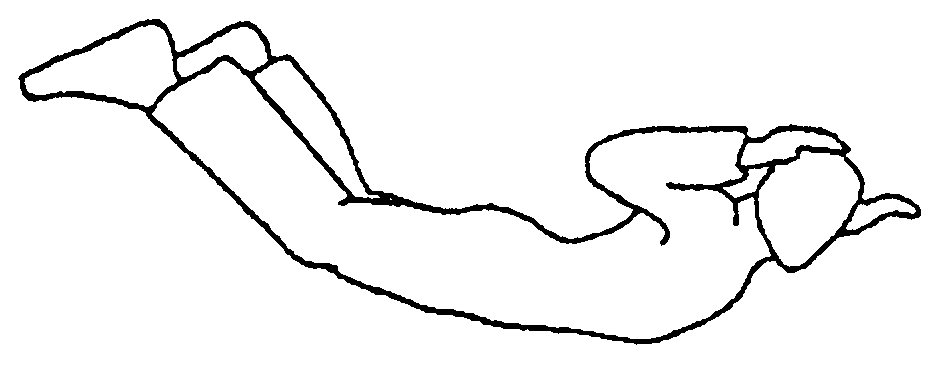
\includegraphics[width=0.7\textwidth]{Asento-liikeeteen.png}\captionof{figure}{Liikkuminen eteen}\end{Figure} 


Liikkuminen taaksepäin tapahtuu työntämällä käsiä eteenpäin ja koukistamalla samanaikaisesti polvia. 


\begin{Figure}\centering\includegraphics[width=0.7\textwidth]{Asento-liiketaakse.png}\captionof{figure}{Liikkuminen taakse}\end{Figure} 

\section{ Liikkuminen alas- ja ylöspäin }
\label{fs-kuviohyppaaminen-liikkuminen-alas-ja-ylospain}


Alas- ja ylöspäin liikkumista käytetään hyppykaverin kanssa samalla tasolla pysymiseen. Katsekontakti pariin täytyy säilyttää koko ajan. Pystysuoraan liikkumiseen käytetään taivutuksen lisäämistä (alaspäin suuntautuva liike) tai negatiivista taivutusta (ylöspäin suuntautuva liike, kupitus). 


\begin{Figure}\centering\includegraphics[width=0.7\textwidth]{Asento-liikeylos.png}\captionof{figure}{Liikkuminen ylös}\end{Figure} \begin{Figure}\centering\includegraphics[width=0.7\textwidth]{Asento-liikealas.png}\captionof{figure}{Liikkuminen alas}\end{Figure} 

\section{ Käännökset }
\label{fs-kuviohyppaaminen-kaannokset}


Paikallaan pysyvä käännös perustuu käsien ja jalkojen samanaikaisiin liikkeisiin; keskivartalo pysyy suorassa linjassa koko käännöksen ajan. Käännös tehdään painamalla toisen puolen kättä ja vastakkaisen puolen jalkaa alaspäin. Käännöksen pysäyttäminen vaatii käsien ja jalkojen nopean ja terävän vastaliikkeen ja sen jälkeen asennon palautuksen perusasentoon. Käyttämällä enemmän käsiä kuin jalkoja saadaan aikaiseksi käännös polvien ympäri. Käyttämällä enemmän jalkoja kuin käsiä saadaan aikaan käännös ylävartalon ympäri. 

\section{ Liikkuminen sivuttain }
\label{fs-kuviohyppaaminen-liikkuminen-sivuttain}


Sivuttaisliikkeen aikaansaamiseksi kallistetaan vartaloa liikkeen suuntaan. Liikkeen pysäyttäminen vaatii vastaliikkeen eli kallistuksen toiseen suuntaan ennen perusasennon palauttamista. 

\section{ Otteiden ottaminen ja kuviossa lentäminen }
\label{fs-kuviohyppaaminen-otteiden-ottaminen-ja-kuviossa-lentaminen}


Otteita otettaessa on aina oltava samalla tasolla sen kanssa, josta otteita otetaan. Otteet otetaan joko ranteista tai gripeistä. Otteen on oltava napakka, mutta siinä ei saa olla vetoa. Ote on muodostelman viimeistelyä/kasaamista, eli hetkellinen pysäytys ennen muodostelman purkua, josta jatketaan seuraavaan muodostelmaan. Otteessa ei roikuta, vaan lennetään aktiivisesti omaa paikkaa ja ollaan valmiina siirtymään seuraavaan muodostelmaan. 

\section{ Hyppyohjelma }
\label{fs-kuviohyppaaminen-hyppyohjelma}


FS-harjoitusohjelma sisältää yhdeksän hyppyä ja niihin liittyvät tekniikat. Kouluttaja valitsee ohjelman hypyistä kyseiseen koulutusvaiheeseen sopivimman. 

\subsection{ Hyppy 1: Liikkuminen eteenpäin }
\label{fs-kuviohyppaaminen-hyppy-1-liikkuminen-eteenpain}


Uloshypyn jälkeen rentoudutaan, otetaan perusasento ja käännytään paria kohti. Lennetään eteenpäin parin luo, otetaan ranneotteet ja perusasento sekä tarkastetaan korkeus. Lennetään kuviossa oikein. Kun pari antaa merkin, päästetään otteet. Pari odottaa 2 sekuntia ja liikkuu muutaman metrin taaksepäin. Toistetaan liike eteenpäin. 


\begin{figure*}[]\centering\includegraphics[width=0.7\textwidth]{FS-1.png}\caption{FS-hyppy 1}\end{figure*} 

\subsection{ Hyppy 2: Liikkuminen eteen- ja taaksepäin }
\label{fs-kuviohyppaaminen-hyppy-2-liikkuminen-eteen-ja-taaksepain}


Uloshypyn jälkeen rentoudutaan, otetaan perusasento ja käännytään paria kohti. Lennetään parin luo ja otetaan ranneotteet ja perusasento. Lennetään kuviossa oikein. Tarkastetaan korkeus ja päästetään otteet kun vetoa ei ole. Odotetaan 2 sekuntia ja liikutaan muutama metri taaksepäin. Toistetaan eteen – taakse -liikettä. 


\begin{figure*}[]\centering\includegraphics[width=0.7\textwidth]{FS-2.png}\caption{FS-hyppy 2}\end{figure*} 

\subsection{ Hyppy 3: Liikkuminen ylös- ja alaspäin }
\label{fs-kuviohyppaaminen-hyppy-3-liikkuminen-ylos-ja-alaspain}


Lennetään parin luo ja otetaan otteet. Tarkastetaan korkeus ja lennetään kuviossa oikein. Pari antaa merkin otteiden irrottamiseksi, kupittaa ja liikkuu ylöspäin metrin. Vähennetään taivutusta, kupitetaan metri ylöspäin parin tasalle ja otetaan perusasento. Pari taivuttaa ja liikkuu metrin alaspäin. Lisätään taivutusta, jotta päästään parin tasalle ja otetaan perusasento. Hypyllä ei oteta enää otteita. Pari pitää etäisyyden hypyn aikana muutamassa metrissä, jotta voidaan kupitettaessa kääntää päätä alaspäin ja silti pitää katsekontakti pariin. Pidetään asento koko ajan symmetrisenä. Toistetaan liikettä. 


\begin{figure*}[]\centering\includegraphics[width=0.7\textwidth]{FS-3.png}\caption{FS-hyppy 3}\end{figure*} 

\subsection{ Hyppy 4: Pystysuora liikkuminen yhdistettynä eteenpäin liikkeeseen }
\label{fs-kuviohyppaaminen-hyppy-4-pystysuora-liikkuminen-yhdistettyna-eteenpain-liikkeeseen}


Lennetään parin luo ja otetaan otteet. Pari peruuttaa pari metriä ja kupittaa ylöspäin metrin. Kupitetaan, lennetään eteenpäin parin luo ja otetaan perusasento. Otetaan otteet ja lennetään kuviossa oikein. Pari peruuttaa pari metriä ja taivuttaa alaspäin metrin. Taivutetaan, lennetään eteenpäin parin luo ja otetaan perusasento. Otetaan otteet ja lennetään kuviossa oikein. Kun tehdään liike, niin pyritään aina ensin liikkumaan pystysuoraan samalle tasolle parin kanssa ja vasta sitten eteenpäin otetta varten. Pidetään katsekontakti pariin koko ajan. Toistetaan liikettä. 


\begin{figure*}[]\centering\includegraphics[width=0.7\textwidth]{FS-4.png}\caption{FS-hyppy 4}\end{figure*} 

\subsection{ Hyppy 5: 90° käännös }
\label{fs-kuviohyppaaminen-hyppy-5-90deg-kaannos}


Käännöksissä paria pidetään kiintopisteenä. Käännökset tehdään puolitähdestä avohaitariin ja siitä takaisin puolitähteen. Lennetään parin luo ja otetaan otteet. Pari antaa merkin, jonka jälkeen irrotetaan vasemman käden ote ja muodostelma avataan 90° puolitähdeksi. Kun otteessa ei ole vetoa, annetaan merkki. Päästettäessä ote odotetaan hetki ennen kuin aloitetaan liike. Käännytään 90° oikealle ja otetaan ote vasemmalla kädellä (avohaitariin). Annetaan merkki ja käännytään takaisin puolitähteen. Pidetään huoli, että otteita otettaessa ollaan samalla tasolla parin kanssa. Kuviosta toiseen liikuttaessa tehdään ensin oikea liike ja vasta sitten otetaan otteet. Kun otetaan ote, varmistetaan, että se on kevyt ja että lennetään paikalla eikä otteessa roikuta. Toistetaan liikettä. 


\begin{figure*}[]\centering\includegraphics[width=0.7\textwidth]{FS-5.png}\caption{FS-hyppy 5}\end{figure*} 

\subsection{ Hyppy 6: 180° käännös }
\label{fs-kuviohyppaaminen-hyppy-6-180deg-kaannos}


Lennetään parin luo ja otetaan otteet. Käännytään 90° oikealle ja pysähdytään ilman otteita olevaan sidebody-muodostelmaan. Pidetään etäisyyttä ja kulmaa 2 sekuntia. Käännytään 180° vasemmalle vastakkaiseen sidebody-muodostelmaan pitäen paria kiintopisteenä. Pidetään etäisyyttä ja kulmaa 2 sekuntia. Pysähdytään käännösten välillä, jotta pystytään keskittymään ja jotta käännökset eivät alkaisi mennä yli halutun astemäärän. Jos ajaudutaan sivuttain poispäin parista, niin käännytään välittömästi paria kohti ja jatketaan käännöksiä toiseen suuntaan. Toistetaan liikettä. 


\begin{figure*}[]\centering\includegraphics[width=0.7\textwidth]{FS-6.png}\caption{FS-hyppy 6}\end{figure*} 

\subsection{ Hyppy 7: 360° käännös }
\label{fs-kuviohyppaaminen-hyppy-7-360deg-kaannos}


Lennetään parin luo ja otetaan otteet. Parin annettua merkin käännytään 360° oikealle. Käytetään jalkoja käännökseen. Muistetaan perusasennon symmetrisyys, aloitus – lähestyminen – pysäytys ja otetaan otteet. Käännytään 360° vasemmalle. Ollaan kärsivällisiä ja odotetaan ennen käännöksen aloittamista, että kuvio on purettu ja että parin kanssa lennetään vierekkäin samalla tasolla. Muistetaan, että liike tulee hidastaa hyvissä ajoin, jottei kääntyminen mene yli halutun astemäärän. Toistetaan liikettä. 


\begin{figure*}[]\centering\includegraphics[width=0.7\textwidth]{FS-7.png}\caption{FS-hyppy 7}\end{figure*} 

\subsection{ Hyppy 8: Liikkuminen sivuttain }
\label{fs-kuviohyppaaminen-hyppy-8-liikkuminen-sivuttain}


Liike tehdään parin edessä aloittaen tähdestä ja liikkuen siitä sivuttain avohaitariin, jonka jälkeen toisen puolen avohaitariin ja taas takaisin tähteen. Lennetään parin luo ja otetaan otteet. Liikutaan oikealle vartalonmitan verran, pysäytetään ja otetaan ote. Liikutaan vasemmalle kahden vartalonmitan verran, pysäytetään ja otetaan ote. Toistetaan liikettä. 


\begin{figure*}[]\centering\includegraphics[width=0.7\textwidth]{FS-8.png}\caption{FS-hyppy 8}\end{figure*} 

\subsection{ Hyppy 9: Lähestyminen sivuttain }
\label{fs-kuviohyppaaminen-hyppy-9-lahestyminen-sivuttain}


Liike tehdään parin edessä aloittaen tähdestä ja tehden 90° käännös oikealle ja sen jälkeen liikkuen sivulle paria kohden, jotta hän saa otteet. Tämän jälkeen pari antaa merkin ja irrottaa otteet. Lennetään parin luo ja otetaan otteet. Käännytään vasemmalle 90° ja liikutaan sivuttain parin luo. Pari antaa merkin ja irrottaa otteet. Muistetaan käyttää koko vartaloa sivuttain liikkeessä. Pyritään tekemään käännökset aina rauhallisesti, jotta ei käännytä yli. Toistetaan liikettä. 


\begin{figure*}[]\centering\includegraphics[width=0.7\textwidth]{FS-9.png}\caption{FS-hyppy 9}\end{figure*} 

\end{multicols}

\chapter{Free-hyppääminen}
\label{free-hyppaaminen}
\thispagestyle{headings}
\begin{multicols}{2}

Freehyppyjen tarkoituksena on perehtyä vapaan lentämisen alkeisiin. Harjoitushyppyjä ei saa ottaa liian vakavasti, sillä tarkoitus on antaa joitakin vinkkejä siitä, miten jatkossa kannattaa harjoitella perusasennosta poistumista. Freekoulutushyppyjen tarkoitus ei niinkään ole opettaa jotain yksittäistä lentoasentoa, vaan tutustuttaa oppilas lentämiseen erilaisissa asennoissa, oppia hallitsemaan vartaloaan muussakin asennossa kuin perusasennossa sekä oppia palautumaan yllättävistä asennoista stabiiliin perusasentoon. Ensimmäinen vaihe freelentämisen harjoittelussa on vatsallaan pysyminen. Kun tämä hallitaan, voidaan ruveta harjoittelemaan muissa asennoissa lentämistä. Seuraavissa teoriaosuuksissa käydään läpi muutamia freeperusasentoja ja -liikkeitä sekä annetaan perusteet niiden harjoitteluun. 

\section{ Sittis }
\label{free-hyppaaminen-sittis}


Katso sittisasennon perusasiat Freeoppaan puolelta (\ref{freefly-lentoasennot-sittiksen-perusasento} s.\pageref{freefly-lentoasennot-sittiksen-perusasento}). Siellä myös vinkkejä asentoon siirtymiseen. 

\section{ Stand up }
\label{free-hyppaaminen-stand-up}


Kun pysytään istuallaan vapaapudotuksessa, on siitä helppo harjoitella seisovaa asentoa eli stand upia. Stand upissa hyppääjä putoaa erittäin suurella nopeudella (korkeuden tarkkailu) seisovassa asennossa kädet sivuille ojennettuina. 


Siirtyminen sittiksestä stand upiin tapahtuu seuraavasti: 

\begin{itemize}
\item  Tarkastetaan korkeus ja viedään jalat alas yhteen. 
\item  Pidetään katse edelleen horisontissa tai hivenen sen alapuolella. Ei katsota missään tapauksessa suoraan alaspäin jalkoihin, sillä se aiheuttaa muutoksen vartalolinjassa. 
\end{itemize}

Pidetään stand upia muutama sekunti ja siirrytään takaisin sittikseen. 

\section{ Palloasento }
\label{free-hyppaaminen-palloasento}


Palloasennolla (ball position / recovery position) tarkoitetaan asentoa, johon freehyppäämisessä pyritään palautumaan, mikäli menetetään asennon hallinta esimerkiksi sittiksessä tai stand upissa. Asennossa hyppääjä käpertyy osittain palloksi, eli vetää jalat sisään ja koukistaa käsiä kyynärvarsista 90 asteen kulmaan eteenpäin, jolloin asento kääntyy putoamaan hieman selälleen takapainoisesti takapuoli maata kohti. Tällä asennolla koetetaan pitää sama putoamisvauhti kuin useimmilla freekuvilla. Recovery positionin käyttäminen lisää turvallisuutta, kun ilmassa on useampia freehyppääjiä. Jos sittiksen kaatuessa hyppääjä stabiloi itsensä suoraan perusasentoon mahalleen, hänen vauhtinsa hidastuu huomattavasti, ja tämä lisää törmäysriskiä. Oppilassuorituksena recovery positionia on hyvä alkaa harjoitella heti alusta alkaen: sittiksen / muun freeliikkeen kaatuessa otetaan recovery position ja pyritään palautumaan siitä takaisin sittikseen painamalla jalkoja ilmavirtaan ja levittämällä asento sittikseen. Recovery positionia voidaan harjoitella esimerkiksi menemällä kyykkyyn ja painamalla rintakehä reisiä vasten ja samanaikaisesti ottamalla käsiä hieman sisään ja kääntämällä kyynärvarret 90 astetta kyynärpäistä eteenpäin. 

\section{ Turvallisuus }
\label{free-hyppaaminen-turvallisuus}


Freehyppyjen turvallisuuteen liittyviä asioita on lueteltu seuraavassa: 

\begin{itemize}
\item  Tarkkaillaan korkeutta, sillä monissa freeasennoissa putoamisvauhti on erittäin kova. 
\item  Lopetetaan harjoittelu viimeistään 1400 metrin korkeudessa ja palataan perusasentoon. 
\item  Selällään tai istualtaan lennettäessä saattaa rintahihnassa oleva korkeusmittari näyttää väärin. Käsimittarin käyttäminen on suositeltavaa. 
\item  Työskennellään aina poikittain lennettyyn hyppylinjaan nähden, sillä monet freeasennot saattavat väärin tehtyinä ruveta ajelehtimaan (liukumaan). Poikittain linjaan nähden työskenneltäessä ei ajelehdita muiden hyppääjien alle tai päälle. 
\item  Freehypyillä on ensiarvoisen tärkeää, että valjaat ovat sopivat, joten sovitetaan valjaat kunnolla ja kiristetään valjaat tiukalle, jotta ne eivät pääse liikkumaan päällä vapaan aikana. 
\item  Kun puetaan varusteita päälle, pidetään huoli siitä, että kaikki ylipitkät valjashihnat on niputettu kumilenkeillä tarpeeksi tiukasti. 
\item  Varmistetaan, etteivät vaatteet pääse kahvojen ja pampuloiden päälle. 
\item  Pidetään huoli, että apuvarjo on tiukasti taskussaan. 
\item  Joskus selällään tai istualtaan lennettäessä reisihihnat saattavat liukua polvitaipeisiin. Tämän estää reisihihnojen välissä haaran kohdalla oleva kumilenkki. Pyydetään kalustohenkilöä ompelemaan kuminauha jalkahihnoihin, jos sellaista ei ole. 
\item  Muistetaan pysyä hypyn etukäteissuunnitelmassa. 
\end{itemize}

Headdown eli pää alaspäin lentäminen on oppilasvarusteilla kielletty! Varusteita ei ole suunniteltu eikä mitoitettu siihen tarkoitukseen. 

\section{ Hyppyohjelma }
\label{free-hyppaaminen-hyppyohjelma}


Harjoitellaan kutakin suoritusta kouluttajan ohjeiden mukaisesti harjoitusvaljaissa tai maassa ennen varsinaista suoritusta. 

\subsection{ Hyppy 1: Puhdas sittisharjoittelu }
\label{free-hyppaaminen-hyppy-1-puhdas-sittisharjoittelu}


Opetellaan istuvaa perusasentoa ja sittisasennon menetyksen yhteydessä palloasennon käyttöä freehypyillä. 

\subsection{ Hyppy 2: Sittis ja raajojen kontrolli }
\label{free-hyppaaminen-hyppy-2-sittis-ja-raajojen-kontrolli}


Poljetaan jaloilla vuoron perään ja heilutellaan käsiä. Tavoitteena on oppia raajojen hallintaa sittisasennossa. 

\subsection{ Hyppy 3: Sittiskäännökset }
\label{free-hyppaaminen-hyppy-3-sittiskaannokset}


Opetellaan sittiskäännöksiä. 

\end{multicols}

\chapter{Kuvunkäsittely oppilaana}
\label{kuvunkasittely-oppilaana}
\thispagestyle{headings}
\begin{multicols}{2}
\section{ Tarkkuushyppy oppilassuorituksena }
\label{kuvunkasittely-oppilaana-tarkkuushyppy-oppilassuorituksena}


Oppilastarkkuuden tarkoituksena on opettaa varjon hallintaa ja kehittää korkeuden ja etäisyyden arviointikykyä. Tavoitteena olisi se, että jatkokoulutusvaiheessa oppilas osaisi laskeutua turvallisesti lähelle suunniteltua pistettä. Ohjauskuviot ja finaalin aloituspiste tulee suunnitella ja käydä mielessä läpi etukäteen. Laskeutumiskuvion voi lentää puolijarruilla, jotta tuulen vaihteluihin voidaan reagoida. Perusosa ajetaan siten, että finaaliin (tuulilinjalle) käännytään tuulesta riippuen 50–100 metriä maalin takana. Finaali aloitetaan noin 100 metrin korkeudesta. Finaalin alussa säädetään lähestymiskulma oikeaksi joko jarruttamalla tai nostamalla. S-mutkia ei saa tehdä etenkään, jos ilmassa on muitakin hyppääjiä. Valmistautuminen loppuvetoon aloitetaan 30–50 metrin korkeudessa, jolloin viimeistään tulee jarrutusta keventää eli käsiä nostaa ylemmäs. Ohjauslenkkejä ei saa nostaa jarrutustilasta täysiliitoon nopeasti, sillä tällöin varjon vajoamisnopeus kasvaa hetkellisesti ja liian matalalla se voi olla kohtalokasta. Turvallisuus on pidettävä kaiken aikaa mielessä. Varjon sakkauttamista on varottava, eikä matalalla saa tehdä jyrkkiä käännöksiä. 

\subsection{ Hypyn suunnittelu }
\label{kuvunkasittely-oppilaana-hypyn-suunnittelu}


Myös tarkkuushypyssä hypyn huolellinen suunnittelu etukäteen on tärkeää. Maassa tulee tarkkailla sääolosuhteiden, erityisesti tuulen suunnan ja voimakkuuden kehittymistä. Muiden hyppääjien suorituksia seuraamalla voi havaita mahdolliset nostavat tai laskevat ilmavirtaukset sekä turbulenssit. Ennen hypylle lähtöä selvitetään uloshyppypaikka, sektori, josta laskeutumisalueelle pääsee sekä alustavasti ohjauskuviot ja finaalin aloituspiste. 

\subsection{ Uloshyppy, avaus ja alkulähestyminen }
\label{kuvunkasittely-oppilaana-uloshyppy-avaus-ja-alkulahestyminen}


Uloshypyn ja avauksen jälkeen alkulähestymisen aikana tulee varmistaa pääsy laskeutumisalueelle. 

\subsection{ Lähestymiskuvio }
\label{kuvunkasittely-oppilaana-lahestymiskuvio}


Lähestymiskuvion aikana maali ja tuulipussi tulee pitää kaiken aikaa näkyvissä. Tuulen suunnan ja voimakkuuden kehittymistä on tarkkailtava koko ajan. Myötätuuli- ja perusosa lennetään puolijarruilla. Perusosan aikana varjoa sivuttain luistattamalla voidaan tarpeen mukaan siirtää finaalin aloituspistettä joko lähemmäksi tai kauemmaksi aiotusta pisteestä. 

\subsection{ Finaali }
\label{kuvunkasittely-oppilaana-finaali}


Finaalipisteessä varjo käännetään tarkasti tuulilinjalle (tuuli on suoraan maalipisteen suunnasta). Jarruilla säädetään lähestymiskulmaa. Varjo pidetään koko ajan vastatuuleen. Valjaissa tulee olla rentona ja suorana. Varjoa ohjataan loppuun asti maalipistettä kohti, mutta ei yritetä väkisin osua maaliin esimerkiksi liian kovalla jarrutuksella tai matalalla käännöksellä. 

\section{ Kuvunkäsittelyhypyt }
\label{kuvunkasittely-oppilaana-kuvunkasittelyhypyt}


Nopeilla varjoilla lentäminen on kuin lentäisi lentokoneella. Niissä on suorituskykyä ja ominaisuuksia, jotka tekevät liikkumisen ilmassa hauskaksi ja oikein käytettyinä entistä turvallisemmaksi, mutta niissä on samalla myös ominaisuuksia, jotka tekevät niistä väärin käytettyinä vaarallisia. Varjon ominaisuudet on tunnettava, jotta sillä voidaan lentää turvallisesti niissä olosuhteissa, jotka valmistajan ja määräysten mukaan mahdollistavat hyppäämisen. Ääriolosuhteet ja maksimiohjausliikkeet eivät sovi yhteen. 


Ääriolosuhteita ja asioita, joita tulisi välttää, ovat 

\begin{itemize}
\item  kova tuuli, erityisesti puuskainen ja turbulenttinen keli 
\item  toisen jättövirtauksessa lentäminen 
\item  pienet laskeutumisalueet 
\item  väsyneenä hyppääminen 
\item  turhien riskien ottaminen. 
\end{itemize}
\subsection{ Huomioitavia asioita }
\label{kuvunkasittely-oppilaana-huomioitavia-asioita}

\subsubsection{ Vapaapudotus }
\label{kuvunkasittely-oppilaana-vapaapudotus}

\begin{itemize}
\item  Hypätään oikeasta uloshyppypaikasta. 
\item  Tarkastetaan sijainti jo vapaan aikana. 
\item  Puretaan oikeassa korkeudessa sekä riittävän korkealla tasoon ja suoritukseen nähden. 
\item  Liu’utaan eroon muista, tarkastetaan ilmatila ja annetaan avausmerkki. 
\end{itemize}
\subsubsection{ Avauksen aikana }
\label{kuvunkasittely-oppilaana-avauksen-aikana}

\begin{itemize}
\item  Avataan riittävän korkealla, stabiilissa asennossa, katse horisonttiin ja olkapäät horisontin tasossa. Ei katsota olan yli apuvarjoa. Jo avauksen aikana kannattaa tarkkailla ilmatilaa muiden varjojen varalta. 
\item  Tehdään päätös: LENTÄÄ / EI LENNÄ (⇒ varavarjotoimenpiteet). 
\item  Laitetaan kädet takimmaisille kantohihnoille, väistetään tarvittaessa (oikealle) ja tarkastetaan ilmatila. 
\item  Ohjataan takimmaisista kantohinnoista ja etsitään muut. 
\item  Tarkastetaan oma sijainti ja korkeus. 
\item  Tarkastetaan irtipäästöpampula ja varavarjon kahvan paikka ja kiinnitys. 
\item  Käännetään takimmaisista kantohinnoista haluttuun lentosuuntaan. 
\item  Tukahdutetaan slider ja avataan puolijarrut. 
\item  Tehdään varjon ohjauskokeilu viimeistään 600 metrin korkeudessa. 
\end{itemize}
\subsubsection{ Lentäminen}
\label{kuvunkasittely-oppilaana-lentaminen}

\begin{itemize}
\item  Katsekontakti 90 \% ympärille (lentosuunta, sivut, alas, ylös ja taakse) ja 10 \% maahan.  
\item  Annetaan muillekin lentotilaa: ei mennä lähelle, jos ei ole etukäteen sovittu. 
\item  Porrastetaan liikenne mahdollisimman ylhäällä, ei vasta laskeutumiskuviossa. 
\item  Huomioidaan väistämisvelvollisuus: varavarjot, hitaammat kuvut, alemmat ja oikealta tulevat. 
\item  Ohjaillaan varjoa rauhallisesti ja keliä tunnustellen (turbulenttisuus). 
\item  Päätetään tarvittaessa ajoissa varalaskupaikka ja laskusuunta. 
\item  Tarkkaillaan korkeutta ja korkeusmenetystä liikkeiden aikana. 
\end{itemize}
\subsubsection{ Varjon varassa törmäämisestä }
\label{kuvunkasittely-oppilaana-varjon-varassa-tormaamisesta}


Uudet punosmateriaalit aiheuttavat törmäämistilanteissa nykyaikaisella varjokalustolla saavutettavilla lentonopeuksilla hyvin suuria vammoja osuessaan ja takertuessaan hyppääjään. Tällaisia punosmateriaaleja on käytössä liki kaikissa nopeissa kuvuissa. 


Ohuita punosmateriaaleja käyttävillä varjotyypeillä törmättäessä on suositeltava toimintamalli palloksi käpertyminen, jolla koetetaan välttää punoksiin takertuminen ja päästään mahdollisesti punosten välistä. 


Pyri estämään törmääminen varjon varassa väistämällä oikealle ja varoittamalla huutamalla. Jos törmäämistä varjon varassa ei voi välttää, niin menetellään seuraavasti: 

\begin{itemize}
\item  Minimoidaan törmäysvauhti jarruttamalla varjoa voimakkaasti. 
\item  Käperrytään palloksi. 
\item  Jos varjot sotkeutuvat: 
	\begin{itemize}
	\item  tarkkaillaan korkeutta 
	\item  keskustellaan toimintajärjestyksestä 
	\item  varmistetaan, että ollaan irti punoksista/kuvusta (käytetään tarvittaessa koukkupuukkoa) ennen varavarjotoimenpiteitä. 
	\end{itemize}
\item  Kahden hyppääjän ei ole turvallista laskeutua yhdellä erittäin raskaasti kuormitetulla päävarjolla. 
\end{itemize}
\subsubsection{ Laskeutuminen }
\label{kuvunkasittely-oppilaana-laskeutuminen}

\begin{itemize}
\item  Noudatetaan laskeutumissääntöjä: kuvion suunta, esteet ja rajoitukset. 
\item  Tarkkaillaan ympäristöä, tuulta ja maata. 
\item  Suunnitellaan loppukuvio ajoissa. Huomioidaan esteet, ihmiset, muu liikenne, turbulenssi ja tuuli. 
\item  Ei tehdä jyrkkiä käännöksiä. 
\item  Valitaan laskeutumisalue (lyhyt, pitkä) taitojen mukaan. 
\item  Ei yritetä väkisin tiettyyn paikkaan, vaan laskeudutaan rauhallisesti ja turvallisesti.  
\item  Tehdään oikeaoppinen loppuveto (\ref{laskeutumistekniikat-oikeaoppinen-loppuveto} s.\pageref{laskeutumistekniikat-oikeaoppinen-loppuveto}). Kaikki liikkeet tehdään rauhallisesti eikä varjoa sakkauteta. Varjo ei anna anteeksi epäsymmetrisyyttä. 
\end{itemize}

Vastatuulen sijaan voidaan tulla mihin suuntaan tahansa tilanteen niin vaatiessa. Tärkeintä on laskeutua vapaaseen suuntaan ilman matalalla tehtyjä jyrkkiä käännöksiä. 

\begin{itemize}
\item  Pidetään ohjaussuunta loppuun asti eikä oteta vastaan kädellä tai jalalla. 
\item  Ei pumpata loppuvedossa ohjauslenkeillä. 
\item  Jos loppuveto tehdään liian korkealla, pidetään ohjauslenkit alhaalla tai löysätään jarrutusta vain hieman. Jalat pidetään tiukasti yhdessä. 
\item  Tarkkaillaan korkeutta, sillä loppuveto perustuu sekä näköhavaintoon että tuntemukseen. 
\end{itemize}
\subsubsection{ Maahantulon jälkeen }
\label{kuvunkasittely-oppilaana-maahantulon-jalkeen}

\begin{itemize}
\item  Tukahdutetaan kupu vetämällä toinen ohjauslenkki alas. 
\item  Tarkastetaan takaa tulevien lentosuunnat. 
\item  Asetetaan ohjauslenkit tarroihin ja avataan slider. 
\item  Kootaan varjo ja poistutaan laskeutumisalueelta. 
\item  Huomioidaan muut hyppääjät ja liikenne koko ajan. 
\end{itemize}

Hyppyohjelman läpivienti edellyttää sopivat sääolosuhteet myös yli 600 metrin korkeudessa, jotta käännökset, sakkauskokeilut jne. voidaan suorittaa turvallisesti eikä ajauduta pois kenttäalueelta. Alle 600 metrin ei tehdä ääriohjausliikkeitä. FXC-12000 ja oppilas-Cypres voivat toimia, mikäli varjon varassa porataan tai tehdään voimakkaita käännöksiä alle 600 metrin korkeudessa. Hyppyohjelman suorittaminen jatkokoulutuksessa kuuluu koulutusohjelmaan. Kuvunkäsittelyhypyillä ei tehdä vapaapudotussuorituksia. 

\subsection{ Hyppy 1 }
\label{kuvunkasittely-oppilaana-hyppy-1}


Tarkoituksena on oppia tuntemaan oman varjon ominaisuudet ja oppia tekemään loppuveto. Hyppykorkeus on 2000 metriä, josta hypätään 8–10 sekunnin vapaa. Ennen jarrujen avausta kokeillaan ohjausta sekä fleeraamista takimmaisista kantohinnoista. Näin voidaan harjoitella nopeaa väistämistä heti avauksen jälkeen. 


Avataan puolijarrut ja etsitään sakkauspiste. Varjoa ei sakata, vaan etsitään jarrujen piste, jossa pieni lisäys aikaansaisi sakkauksen. Jos varjo sakkaa, nostetaan ohjauslenkkejä ylös hitaasti ja symmetrisesti.  


Tämän jälkeen harjoitellaan loppuvetoa täysiliidosta. Muistetaan terävä alkuveto ja lisätään sen jälkeen jarrutusta vähitellen lähelle sakkauspistettä. Huomioidaan lisääntyvä G-voima ja varjon siirtyminen vaakalentoon. 


Kokeillaan 90 asteen käännöksiä täysiliidosta ja huomioidaan korkeuden menetys ja ilmanopeuden kasvu verrattuna oppilasvarjoon. Valmistaudutaan alastulokuvioon huomioiden porrastukset. Tehdään oikeaoppinen loppuveto täysiliidosta. 

\subsection{ Hyppy 2 }
\label{kuvunkasittely-oppilaana-hyppy-2}


Hyppykorkeus on 2000 metriä, josta hypätään 8–10 sekunnin vapaa. Avataan puolijarrut. Kokeillaan rauhallisia käännöksiä eri lentotiloissa (puolijarrutus, täysijarrutus) molempiin suuntiin. Kokeillaan käännöksiä takimmaisista kantohihnoista molempiin suuntiin. Ei kuitenkaan päästetä ohjauslenkkejä käsistä. 


Kokeillaan nopeaa 360 asteen käännöstä (poraamista) ja pysäytystä ennalta päätettyyn suuntaan. Huomioidaan, kuinka ilmanopeus kasvaa ja korkeus vähenee nopeasti. Huomioidaan kuinka paljon aikaisemmin käännös täytyy lopettaa, että pysäytys tapahtuu valittuun suuntaan, ja kuinka suuri vastaliike täytyy tehdä, että käännös pysähtyy. Seurataan korkeuden menetystä käännösten aikana. (HUOM. Jos varjossa on FXC-12000 tai oppilas-Cypres, ei poraamista saa tehdä alle 600 metrin korkeudessa, koska varavarjon automaattilaukaisin voi toimia). 


Valmistaudutaan alastulokuvioon ja tehdään oikeaoppinen loppuveto täysiliidosta. 

\subsection{ Hyppy 3 }
\label{kuvunkasittely-oppilaana-hyppy-3}


Uloshyppykorkeus ja vapaa ovat samat kuin edellisissä hypyissä. Harjoitellaan loppuvetoa puolijarrutustilasta. Tullaan havaitsemaan, että tarvittava veto on terävämpi kuin täydestä liidosta. Finaali ja loppuveto tehdään puolijarrutustilasta. 

\end{multicols}

\chapter{Omiin varusteisiin siirtyminen}
\label{omiin-varusteisiin-siirtyminen}
\thispagestyle{headings}
\begin{multicols}{2}

Laskuvarjot ja niiden suorituskyky kehittyvät jatkuvasti. Oppilasvarjot on kuitenkin kautta aikojen suunniteltu käyttövarmoiksi ja virheitä anteeksiantaviksi lentolaitteiksi. 1970-luvulla oppilaat hyppäsivät alkeispallovarjoilla. 1980-luvulla oppilaat käyttivät tehovarjoja ja kokeneemmat hyppääjät liitovarjoja. 1990-luvun alussa oppilasvarjoissa siirryttiin F-111-kankaisiin sekä suuriin, korkeaprofiilisiin varjoihin kuten Manta ja Raider. 1990-luvun lopulla ja 2000-luvun alussa alettiin käyttää ZP-kankaisia, lievästi elliptisiä oppilasvarjoja (esim. Navigator, Skymaster). Ne ovat kevyempiä ohjata ja säilyttävät lento-ominaisuutensa pidempään kuin edeltäjänsä. 


Kelpoisuushyppääjien käyttämät varjot ovat vuosien kuluessa kehittyneet nopeammin kuin oppilasvarjot. Käytetyt siipikuormat ovat kasvaneet ja varjomallit kehittyneet jatkuvasti. Monelle jo siirtymä oppilasvarjosta omaan varjoon voi olla melko suuri. On hyvä muistaa, että suuremmalla siipikuormalla lentäminen vaatii paljon keskittymistä turvallisen lentämisen opetteluun.  


Hyppääjän on osattava valita varjonsa ominaisuudet omien kykyjensä, harrastamansa lajin ja hyppy-ympäristönsä mukaan. Varjolla lentämisen tulee olla mukavaa ja turvallista sekä itselle että muille ilmassa oleville. Lisäksi hyppääjän tulee olla ymmärtää oman varjonsa ominaisuudet erilaisissa tilanteissa. Siksi onkin tärkeää tutustua tämän oppaan osaan Kuvunkäsittelyopas, kun siirrytään oppilaskalustosta nopeampiin varjoihin. 

\section{ Laskuvarjoja koskevat kokemusrajat }
\label{omiin-varusteisiin-siirtyminen-laskuvarjoja-koskevat-kokemusrajat}


Jatkokoulutuksessa oleva oppilas voi saada koulutuspäälliköltä tai apulaiskoulutuspäälliköltä luvan käyttää omia varusteitaan ja laskuvarjoaan. SIL ylläpitää luetteloja, joista ilmenee, mitkä varjomallit ovat soveltuvia 

\begin{itemize}
\item  alkeis- ja peruskoulutuksessa oppilaiden käyttöön 
\item  jatkokoulutuksessa oppilaiden käyttöön (koulutuspäällikön/apulaiskoulutuspäällikön suostumuksella)  
\item  itsenäisillä lisenssihyppääjillä  
\end{itemize}

SIL on määritellyt hyppääjille siipikuormarajat (katso siipikuorman määrittely) kokemuksen mukaan seuraavasti: 

\begin{itemize}
\item  alkeis- ja peruskoulutusvaihe < 1,1 lbs/ft². 
\item  jatkokoulutusvaihe sekä A- ja B-lisenssit < 1,34 lbs/ft². 
\end{itemize}

Koulutus- ja turvallisuuskomitea suosittelee jatkokoulutusvaiheen oppilaille ja ensimmäistä varjoaan hankkiville hyppääjille korkeintaan 1,1 siipikuormaa. 


Kelpoisuushyppääjien käytössä olevien varjojen erot oppilasvarjoihin ovat seuraavia: 

\begin{itemize}
\item  pienempiä, suurempi siipikuorma ⇒ suurempi nopeus alas- ja eteenpäin, kasvanut vajaatoimintaherkkyys, suurempi sakkausnopeus ⇒ vaativat suurempaa tarkkuutta ja reaktionopeutta 
\item  siipiprofiililtaan ja muodoltaan suorituskykyisempiä ⇒ parempi liitosuhde, suurempi nopeus ja käännösherkkyys 
\item  ohuet microline-punokset ⇒ välittävät avausnykäyksen voimakkaammin, kuluvat nopeammin, vaaralliset törmättäessä varjon varassa 
\item  lisävarusteet (tukahdutettava slider ja tukahtuva apuvarjo) vaativat huolellisuutta pakkaamisessa ja lentämisessä. 
\end{itemize}

\begin{figure*}[]\centering\includegraphics[width=0.7\textwidth]{MARD.jpg}\caption{MARD-järjestelmä voi nopeuttaa varavarjon avautumista. (kuva: UPT)}\end{figure*} 

\section{ Muut varusteet }
\label{omiin-varusteisiin-siirtyminen-muut-varusteet}


AAD (Automatic Activation Device) eli varavarjon automaattilaukaisin on oppilasvarjoissa sekä A- ja B-lisenssin hyppääjillä pakollinen varuste ja on nykyään vakiovaruste lähes kaikissa uusissa Suomeen tilattavissa varjopaketeissa. AAD:n käyttö kaikessa hyppäämisessä on erittäin suositeltavaa.  


Uusimmilla ja nopeimmilla varjoilla on hetkellisesti saavutettu pystynopeuksia, jotka ylittävät AAD:n virittymiskynnyksen (esimerkiksi expert-Cypresilla 35 m/s). AAD:n aktivoituminen vauhditetussa laskeutumisessa ei kuitenkaan ole mahdollista kuin suurilla siipikuormilla. AAD on pelastanut maailmalla jo satoja hyppääjiä. SIL on luetteloinut Suomessa käyttöön soveltuvat automaattilaukaisimet. 


RSL (Reserve Static Line) tarkoittaa varavarjon pakkolaukaisuhihnaa. Sen tarkoituksena on varmistaa varavarjon avautuminen päävarjon irrottua valjaista. Järjestelmä liittää päävarjon kantohihnan ja varavarjon aukaisujärjestelmän yhteen. RSL on hyvä apuväline, joka voi pelastaa hengen esimerkiksi matalan päävarjon irtipäästön jälkeen. Oppilasvarjoissa sekä A- ja B-lisenssihyppääjille RSL on pakollinen varuste. 


RSL-järjestelmään on saatavissa myös MARD-modifikaatio (Main assisted reserve deployment). MARD-järjestelmässä irti päästetty päävarjo avustaa varavarjon avautumista. Tämä nopeuttaa varavarjon avautumista ratkaisevasti. Tilanteissa, joissa irti päästetty päävarjo ei pysty nopeuttamaan varavarjon avautumista, RSL toimii normaalisti. MARD-järjestelmät ovat valmistajakohtaisia (esim. DRD, Reserve boost ja Skyhook), eikä niitä välttämättä ole saatavilla kaikkiin valjaisiin. RSL:n hihnan tulee olla kytkettynä, jotta MARD voi toimia. 


Kypärän/suojapäähineen käyttö on pakollista D-lisenssiin asti. Myös D-lisenssihyppääjät käyttävät yleensä hypätessään kovaa kypärää. Jos myöhemmin A-lisenssin saatuasi alat harjoitella nopeita laskeutumisia, käytä aina kovaa kypärää. 


Sopivan kypärän valintaan vaikuttaa esimerkiksi hyppylaji. Avokypärä mahdollistaa hieman laajemman näkökentän, mutta integraalikypärä suojaa mahdollisessa törmäyksessä myös hyppääjän leukaa ja kasvoja. Integraalikypärää käyttäessä kannattaa huomioida, että suljettu visiiri voi välillä huurtua. Visiirin avaamista ja sulkemista on syytä harjoitella etukäteen. Esimerkiksi tavallista paksummat käsineet voivat vaikeuttaa visiirin avaamista kuvun varassa.   


Useimmat hyppääjät käyttävät käsikorkeusmittaria. Mittarin voi sijoittaa kuitenkin myös muualle kuin ranteeseen. Analogisen korkeusmittarin voi esimerkiksi kiinnittää rintahihnaan. Digitaalista, numeronäyttöistä mittaria voi puolestaan käyttää reiteen tai käsivarteen kiinnitettynä. Tärkeintä mittarin käytössä on se, että käytetään aina samassa paikassa olevaa mittaria ja opetellaan lukemaan visuaalista mittaria kaikissa lentoasennoissa sekä kuvun varassa.  


Monet hyppääjät käyttävät visuaalisen mittarin lisäksi äänikorkeusmittaria. Niissä on usein 2–3 säädettävää hälytysrajaa, jotka hyppääjä voi asettaa haluamiinsa korkeuksiin. Äänikorkeusmittarit voivat myös tallentaa tietoa esimerkiksi hyppykorkeudesta, vapaapudotusajasta ja -nopeudesta sekä avauskorkeudesta. 


Äänikorkeusmittarit ovat hyvin luotettavia ja ne ovat hyödyllisiä lisävarusteita lähes kaikessa hyppäämisessä. Eritoten freehyppäämisessä, kameran tai muun lisälaitteen kanssa hypätessä äänikorkeusmittari on liki pakollinen varuste.  Äänikorkeusmittari on kuitenkin vain varmistusväline, korkeutta on jokaisella hypyllä tarkkailtava myös visuaalisesta mittarista.  


Korkeusmittarit ovat kaiken kaikkiaan hyvin luotettavia laitteita, mutta korjaus, huolto sekä paristojen vaihto takaavat mittarin toimivuuden. Mittarit on syytä huollattaa aina asiantuntijalla. 


Kameran kanssa hyppääminen on yleistynyt huomattavasti kameroiden koon pienentyessä ja hintojen halventuessa. Tällä hetkellä kameran kanssa hyppäämiseen vaaditaan C-lisenssi, mutta aina ennen kuvaushyppäämisen aloittamista on keskusteltava kerhon turvallisuuspäällikön sekä kokeneiden kuvaushyppääjien kanssa tarvittavista taidoista sekä kamerakypärän rakentelusta. Turvallinen kuvaushyppääminen vaatii huomattavaa paneutumista asiaan niin tiedollisesti kuin taidollisestikin. Äänikorkeusmittarin käyttäminen kuvaushypyillä on erittäin suositeltavaa. 


Liki jokaiseen hyppylajiin on olemassa erityisesti siihen lajiin suunniteltuja haalareita. FS-haalareissa on tyypillisesti grippejä otteiden ottamisen helpottamiseksi sekä useimmiten \textit{bootit} liu’un sekä jalkatyöskentelyn tehostamiseksi. Freehyppääjät suosivat haalareita, jotka soveltuvat eri asennoissa lentämiseen. Jos käytät aluksi hyppyasuna housuja ja paitaa, varmista ettei paidan helma missään asennossa pääse kääntymään avauskahvan tai irtipäästö- ja varavarjokahvojen päälle. 


Hyppääjä voi hypätä erilaisten lisävarusteiden kanssa, seuraavassa muutamia ominaispiirteitä: 

\begin{itemize}
\item  Liitopuku: Liitopuvulla hyppääminen vaatii joko C-lisenssin ja koulutuksen tai D-lisenssin. Lue lisää asiasta Liitohyppyoppaasta. 
\item  Savut, liput ja viirit: Näytöshypyillä saattaa joskus tulla tarpeen käyttää esimerkiksi savuja, lippuja tai viirejä lisäämään näytöksen näyttävyyttä. Hypättäessä lipun tai viirin kanssa tulee aina miettiä, onko lippu tai viiri \textit{vapaapudotukseen oleellisesti vaikuttava varuste}, jolloin sen kanssa hyppääminen vaatii D-lisenssin. Savujen, lippujen ja viirien virittely vaatii paljon kokemusta, joten pyydä apua kokeneemmilta hyppääjiltä. Savujen käytöstä on aina sovittava lentäjän (lennonjohdon) kanssa. 
\item  Skysurf: Lautahyppääminen vaatii joko C-lisenssin  ja koulutuspäällikölle annettavat käytännön taitonäytteet, joilla osoitetaan, että omataan lautahyppäämiseen tarvittavat perustaidot tai D-lisenssin. Lue lisää asiasta Skysurf-alkeisoppaasta. 
\item  Spaceball: Spaceballin kanssa hyppääminen on Suomessa kiellettyä. 
\end{itemize}
\section{ Harjoitus ja harjoitushypyt }
\label{omiin-varusteisiin-siirtyminen-harjoitus-ja-harjoitushypyt}

\begin{enumerate}[label=\bfseries \arabic*)]
\item  Tutustutaan Laskuvarjohyppääjän oppaan Kuvunkäsittelyoppaaseen ja aiheeseen liittyviin turvallisuusmääräyksiin ja tiedotteisiin. 
\item  Suoritetaan sopivan siipikuorman arviointi ja päävarjon koon ja tyypin valinta sekä pohditaan varuste- ja varjovaihtoehtoja huomioiden mahdolliset rajoitukset. 
\item  Harjoitellaan ja kerrataan koulutushypyillä tehtävät suoritukset. 
\item  Annetaan näyte hyppymestarille varjon avautumisen jälkeisistä toimenpiteistä ja toiminnasta törmäämistilanteessa. 
\end{enumerate}
\end{multicols}

\chapter{Kaluston tarkastus ja huolto}
\label{kaluston-tarkastus-ja-huolto}
\thispagestyle{headings}
\begin{multicols}{2}
\section{ Asiakirjojen tarkastus }
\label{kaluston-tarkastus-ja-huolto-asiakirjojen-tarkastus}


Ostettavan varjokokonaisuuden laitekortit on aina tarkastettava huolellisesti. Apua laitekorttien tarkastukseen kannattaa pyytää kerhon kalustohenkilöiltä tai hyppymestareilta. Laitekortit voivat olla reppu-valjasyhdistelmässä tai varjoissa uudelleen avattuja. Tällaisissa tapauksissa laitekorteista ei selviä todellinen käyttö- ja huoltohistoria. Käyttö- ja huoltohistorian ollessa epäselvä on syytä suhtautua ostamiseen terveellä epäluulolla. 


Laitekortista on tarkastettava aina seuraavat kohdat ja niitä on verrattava kalustoon: 

\begin{itemize}
\item  Varjon ja valjaiden tyypin, sarjanumeroiden ja valmistusmerkintöjen eli tunnistetietojen on täsmättävä laitekortissa oleviin. Kupujen tunnistetiedot löytyvät kuvun takahelmassa olevasta varoituslapusta. Valjaissa tunnistetiedot on yleensä merkitty joko varavarjon kantohihnassa tai repun niskassa ommeltuna olevaan merkkiin. Merkin sijainti vaihtelee repun valmistajan mukaan. Tunnistetietojen vertailuun ja merkin löytämiseen on hyvä pyytää apua kerhon kalustohenkilöiltä tai hyppymestareilta. 
\item  Tunniste- ja rekisteröintitiedot ovat luettavissa laitekortista. 
\item  Varjon omistajan vaihdoksesta tekee vanha omistaja merkinnän laitekorttiin.   
\item  Varjoihin ja reppu-valjasyhdistelmään tehdyt tarkastukset, huollot, korjaukset sekä lentokelpoisuusmääräysten edellyttämät työt näkyvät laitekortista. Seuraavan tarkastuksen ajankohta kannattaa huomioida, ja jos mahdollista, käytetty varjo tai reppu-valjasyhdistelmä kannattaa tarkastuttaa ennen ostamista. 
\item  Varavarjo ja reppu-valjasyhdistelmä tarkastetaan aina yhdessä. Varavarjon ja valjaat voi tarkastaa kalustomestari C:n pätevyyden omaava henkilö. Päävarjo tarkastetaan aina kiinnitettynä reppu-valjasyhdistelmään. Päävarjon voi tarkastaa kalustomestari B tai C. Kalustomestari B:n tai C:n on tarkastettava päävarjo myös uuteen reppu-valjasyhdistelmään ennen kuin päävarjolla voidaan hypätä. 
\item  Varavarjon pakannut henkilö merkitsee aina laitekorttiin varavarjoon tehtävät toimenpiteet kuten pakkaukset ja käytönjälkeiset tarkastukset. 
\item  Päävarjon pakkausmerkinnäksi riittää hyppypäiväkirjamerkintä.  
\item  Automaattilaukaisimen laitekortista selviää laitteen tunnistetietojen lisäksi huoltotilanne ja mahdollinen pariston vaihdon ajankohta. 
\item  Ostettaessa pelkästään vara- tai päävarjoa tai valjaita on huomioitava, että pää- ja varavarjo sisältävät connectorilenkit, kantopunokset, sliderin ja itse varjon. Reppu-valjasyhdistelmään kuuluvat apuvarjo yhdyspunoksineen, kantohihnat sekä päävarjon ja varavarjon sisäpussi. 
\end{itemize}

Käytettyä tai uutta varjokokonaisuutta ostettaessa on harkittava tarkkaan, mitkä ovat omat lajimieltymykset ja mikä on todellinen hankintatarve. On myös hyvä miettiä, tarvitaanko kalliimpi, uusi varjo, vai riittääkö alkuun edullisempi, käytetty varjo. 

\section{ Kuntotarkastus }
\label{kaluston-tarkastus-ja-huolto-kuntotarkastus}


Käytetty varjo tai varjokokonaisuus kannattaa kuntotarkastuttaa kalustohenkilöllä säännöllisesti ja aina ennen ostopäätöstä. Koehyppäämällä ja tarkistuttamalla voidaan todeta varjokankaan mahdollinen ilmanläpäisyn lisääntyminen ja punosten venymisestä johtuvat ominaisuuksien heikkenemiset. Kuntotarkastuksessa selviää kaluston mahdollinen korjaustarve, mikä auttaa omalta osaltaan hinnan määrityksessä. Samalla on myös hyvä määrittää kokonaisuuden sopivuus ostajan päälle, ettei tule hankituksi liian isoa tai liian pientä reppu-valjasyhdistelmää. 


Kuntotarkastusta tehtäessä etsitään vikoja ja käytöstä johtuvia kulumajälkiä valjaista, repusta, pää- ja varavarjosta. Rispaantuneet paineentasaukkojen reunat, ohjauspunosten alapäiden ja reisihihnojen kulumiset ovat näkyvimpiä ja yleisimpiä käytöstä johtuvia kulumisen kohteita. Varjokokonaisuuden kulumiseen vaikuttavia asioita ja seurattavia kohteita: 

\begin{itemize}
\item  Punokset kuluvat nopeasti kuluneiden sliderin renkaiden takia. Punossetti kestää yleensä 500–700 hyppyä. Punosten epätasainen kutistuminen aiheutuu sliderin tuottamasta kitkalämmöstä ja huonontaa varjon lento- ja avautumisominaisuuksia. 
\item  Avausjärjestelmään sekä kupuun tulee palamisreikiä huolimattoman pakkauksen vuoksi. Valmistajan ohjeiden mukainen pakkaus säästää kupua. 
\item  Ompeleet ja varjokangas kuluvat lian ja roskien vaikutuksesta. 
\item  Valjaiden kulumista ja likaantumista lisää ilman pakkausalustaa pakkaaminen. 
\item  Kuluvia osia, kuten ohjauspunosten alapäitä, paineentasausaukkojen reunoja, avausjärjestelmän osia, sliderin renkaita sekä mahdollisia tarroja on tarkkailtava ja niiden vaihdattaminen tai korjauttaminen kannattaa suorittaa ajoissa muiden osien säilymiseksi. 
\end{itemize}

Määräaikaistarkastusten yhteydessä suoritettavat korjaukset ja osien vaihdot voivat tuntua kalliilta, mutta ne takaavat varjokokonaisuuden toimivuuden ja hyppyturvallisuuden. Korjaukset ja vaihdot saa suorittaa vain kalustomestari B tai C pätevyytensä mukaisesti. 

\section{ Huolto }
\label{kaluston-tarkastus-ja-huolto-huolto}


Päivittäiseen kalustohuoltoon kuuluu 

\begin{itemize}
\item  kierteiden poisto ohjauspunoksista ja yhdyspunoksesta 
\item  päävarjon luupin kunnon ja pituuden tarkastus ja tarvittaessa vaihto uuteen 
\item  irtohiekan ja muun mahdollisen lian poistaminen päävarjosta ravistamalla takahelmasta 
\item  sisäpussin kuminauhojen vaihtaminen ehjiin ja valjaskuminauhojen kunnon tarkastaminen 
\item  repun ja valjaiden puhdistus irtoliasta tarvittaessa esimerkiksi juuriharjalla 
\item  varusteiden kuivaus tarvittaessa sekä oikea säilytys suojassa valolta, lialta ja kosteudelta. 
\end{itemize}

Varusteiden huollossa ja säilyttämisessä on huomioitava myös seuraavat seikat: 

\begin{itemize}
\item  Kuvun ja valjaiden pesua kannattaa välttää. Pakottavissa tilanteissa pesu on mahdollinen, mutta asiassa kannattaa kääntyä kalustohenkilön puoleen turvallisen pesutavan selvittämiseksi. 
\item  Ei säilytetä varjoa auton takakontissa ilman varjokassia. 
\item  Luupin on oltava ehjä ja oikean pituinen. 
\item  Kerhon säilytystilat on pidettävä kuivina, eikä niissä saa säilyttää mitään syövyttäviä tai paloarkoja aineita. 
\item  Varjoa säilytetään talven yli kotona kuivassa ja pimeässä paikassa. Kuiva varjo voi olla sisäpussissaan, mutta varavarjon jousiapuvarjo on hyvä vapauttaa, mikäli säilytys on pitempiaikaista.  
\end{itemize}

Kun kalusto on kunnossa, voidaan hypätä turvallisesti. Kalusto huolletaan itse päivittäin ja toimitetaan kalustohenkilölle heti, jos siinä epäillään vähäistäkin kulumista tai vikaa. Tarkastamattomalla ja huoltamattomalla kalustolla ei saa hypätä. Kalustosta kannattaa pitää huolta, sillä ajoissa tehdyt huollot säästävät isommilta vaurioilta ja kalliilta korjauksilta. 

\section{ Harjoitus }
\label{kaluston-tarkastus-ja-huolto-harjoitus}

\begin{enumerate}[label=\bfseries \arabic*)]
\item  Tutustutaan varjokirjoihin ja laitekortteihin. 
\item  Suoritetaan varjon ja reppu-valjasyhdistelmän kuntotarkastus ja päivittäinen huolto pakkauksen yhteydessä. 
\end{enumerate}
\end{multicols}

\chapter{Pakkaustarkastus}
\label{pakkaustarkastus}
\thispagestyle{headings}
\begin{multicols}{2}

Ennen laskuvarjon pakkausta on hypyn jälkeen palautettava muut hypyllä tarvitut varusteet omille paikoilleen. Näin ne ovat muiden käytössä, eivätkä ne rikkoonnu pakkaustilan lattialla. Laskuvarjon pakkausta edeltää myös varjon selvittäminen ja puhdistaminen hiekasta ja irtoliasta. Jos varjossa havaitaan vikaa ennen pakkausta tai sen aikana, on asiasta välittömästi ilmoitettava hyppymestarille tai kalustopäällikölle. Viallista tai märkää varjoa ei saa pakata! Pakkauskirja on esitäytettävä valmiiksi ja pakkauksessa noudatetaan aina huolellisuutta. Kun varjo pakataan oikein, se toimii ja säilyy ehjänä ja käyttökelpoisena pidempään. Vastuu pakkauksesta on sekä pakkaajalla että pakkaustarkastajalla. Tarkastuksen saa suorittaa A-D-lisenssihyppääjä. Pakkaustarkastuksesta on muistettava, että se on aina opetus- ja oppimistapahtuma. 


Pystypakkaus I tarkastusvaiheeseen suoritetaan seuraavasti: 


Tarkistetaan ohjauspunosten selvyys koko matkalta ohjauslenkistä kuvun takahelmaan, poistetaan kierteet ohjauspunoksista ja kiinnitetään puolijarrut. Nostetaan kupu olkapäälle, laitetaan 9 tunnelin suuta polvien väliin, viikataan A\mbox{-,} B\mbox{-,} C- ja D-punosryhmien välistä kankaat sivulle stabilisaattoriväleihin. Taitellaan kuvun takahelma ohjauspunosten välistä sivulle, muiden punosryhmien päälle, lasketaan slider tähden muotoon stabilisaattorien kovikkeita vasten. 

\section{ I tarkastusvaihe }
\label{pakkaustarkastus-i-tarkastusvaihe}


I tarkastusvaiheen tarkastaja vastaa siitä, että 

\begin{itemize}
\item  Repun, valjaiden ja varjon yleiskunto sekä siisteys on hyvä. 
\item  Repun luuppi ja avausjärjestelmän varusteet ovat kunnossa, slider ja apuvarjo on viritetty. 
\item  PL-hihna, lukko ja sokka/IA-kahva ovat kunnossa, eikä niissä ole kulumia. 
\item  Olkalukot ovat maata kohti eivätkä kantohihnat ole kierteellä. 
\item  Olkalukot ovat kiinni ehjillä luupeilla ja connectorilenkkien suojat ovat kiinni ja ehyet. 
\item  Puolijarrut on kiinnitetty, ohjauslenkkien päät on työnnetty käärmeensilmien läpi ja lenkit ovat kiinni tarroissaan ja taskuissaan. 
\item  Ylimääräinen ohjauspunos on lenkitetty siististi ja taiteltu kiinnitystarrojen (tai vastaavien) alle. 
\item  Ohjauspunokset ovat koko pituudeltaan erillään muista punoksista. 
\item  Kupu on laskostettu molemmilta puolilta stabilisaattoriväleihin siististi. 
\item  Takahelma on laskostettu ohjauspunosten välistä sivulle. 
\item  Punokset ovat tiukalla kuvun keskellä: 4+4 ohjaus\mbox{-,} 5+5 D\mbox{-,} 5+5 C\mbox{-,} 5+5 B- ja 5+5 A-punosta. 
\item  Slider on taitettuna kuvun sisälle ristiin, purjerenkaat nipussa. 
\item  Etuhelman 9 tunneliparia on tasattu. 
\end{itemize}

Tarkastuksen on oltava yksityiskohtainen, jotta pakkausta ei tarvitse keskeyttää myöhemmin puutteen tai vian takia. Tämän jälkeen tarkastaja kuittaa ensimmäisen tarkastusvaiheen pakkauskirjanpitoon todeten samalla esitäytettyjen pakkaustietojen paikkansapitävyyden. 


Pakkaus II tarkastusvaiheeseen suoritetaan seuraavasti: 

\begin{itemize}
\item  Asetetaan takahelman keskiosa ylös (warning label / keskimerkki) sliderin purjerenkaiden päälle ja kiedotaan niiden ympärille. 
\item  Kierretään takahelman reunat kuvun ympäri, vapautetaan tunnelinsuut jalkojen välistä, tasataan tunnelin suut kuvun reunan tasalle sekä kiristetään takahelman reunat ja rullataan 5–6 kierrosta. 
\item  Asetetaan kupu maahan punokset kireällä, poistetaan ilma kuvusta ja muotoillaan se hieman sisäpussia leveämmäksi pötköksi, taitetaan kuvun alaosa kuvun s-mutkalle ja kuvun yläosa edellisen taitoksen päälle sekä sujautetaan kupu sisäpussiin.  
\item  Vedetään ylimääräinen yhdyspunos pois sisäpussista ja tarkistetaan, ettei varjokangasta jää sisäpussin purjerenkaan ja yhdyspunoksen väliin.  
\item  Suljetaan sisäpussi purjerenkaiden kautta kulkevilla yksinkertaisilla kumilenkeillä ja punostetaan loput punokset kumilenkeillä kireälle. 
\end{itemize}
\section{ II tarkastusvaihe }
\label{pakkaustarkastus-ii-tarkastusvaihe}


II tarkastusvaiheen tarkastaja vastaa seuraavista asioista: 

\begin{itemize}
\item  Kupu on sisäpussissa tasaisesti ja pursuilematta. 
\item  Yhdyspunos on vedetty ulos sisäpussista kiinnitysrenkaaseen saakka eikä varjokangasta ole purjerenkaan ja yhdyspunoksen välissä. 
\item  Yhdyspunoksessa/pakkolaukaisuhihnassa ei ole kierrettä. 
\item  Punostus on tasainen ja kireä. 
\item  Toisen vaiheen tarkastaja vastaa myös (pakkaajan ohella) repun oikeasta sulkemisesta: 
	\begin{itemize}
	\item  Sisäpussi asetetaan reppuun oikein ja pyörittämättä. 
	\item  Kantohihnat tulevat taskuihinsa suoraan ja riittävän syvälle eikä niitä ole taitettu varavarjon repun pohjaa vasten. 
	\item  Ohjauslenkit ovat pysyneet kiinni tarroissaan ja taskuissaan. 
	\item  Apuvarjo ja yhdyspunos taitellaan ja pakataan oikein. 
	\item  Reppu suljetaan käsikirjan mukaisesti ja paranaru poistetaan. 
	\item  Viimeistellään pakkaus siistiksi. PL-hihna taitellaan lenkkeihinsä ja viedään varjo paikoilleen. 
	\end{itemize}
\end{itemize}

Tämän jälkeen tarkastaja kuittaa toisen tarkastusvaiheen pakkauskirjanpitoon. 

\section{ Harjoitus }
\label{pakkaustarkastus-harjoitus}

\begin{enumerate}[label=\bfseries \arabic*)]
\item  Harjoitellaan oppilaspäävarjon pakkaustarkastuksen tekemistä jokaisella pakkauskerralla tämän koulutuksen jälkeen. 
\item  Huomioidaan tarkastuksissa olevat erot eri avausjärjestelmillä olevissa varjoissa: pakkolaukaisu, jousi- ja HD-apuvarjo. 
\end{enumerate}
\end{multicols}

\chapter{Määräykset, lait ja ohjeet}
\label{maaraykset-lait-ja-ohjeet}
\thispagestyle{headings}
\begin{multicols}{2}

Laskuvarjotoimintaa ja -hyppääjiä koskevat lait, asetukset, määräykset, koulutusohjelmat, ohjeet ja tiedotteet on laadittu luomaan selvät pelisäännöt lajin harrastamiseksi sekä ehkäisemään onnettomuuksia. Trafin hyväksymien ilmailumääräysten ja -tiedotusten lisäksi Suomen Ilmailuliitto ry on laatinut hyppääjille koulutusohjelmat ja tomintaohjeet. Lisäksi Ilmailuliiton  Laskuvarjotoimikunta ja sen komiteat julkaisevat ohjeita, suosituksia ja tiedotteita, jotka on myös huomioitava. 


Ohjeen tai vastaavan ja määräyksen ollessa ristiriidassa on määräys aina se asiakirja, jota noudatetaan. Kuitenkin ohjeessa tai muussa vastaavassa voidaan tiukentaa määräyksien vaatimuksia. Samoin kerhoilla on oikeus tiukentaa annettuja ohjeita ja määräyksiä omaa toimintaansa varten. 


Asiakirjat on luettava ja ne tentitään kelpoisuushyppytoimintaa koskevilta osin ennen A-lisenssin hakemista. Ainakin seuraavat ajan tasalla olevat asiakirjat on oltava luettavissa kerholla koko koulutusajan, ja niihin tulee tutustua myös päivitysten yhteydessä. 

\section{ Lait ja asetukset }
\label{maaraykset-lait-ja-ohjeet-lait-ja-asetukset}

\begin{itemize}
\item  Ilmailulaki 22.12.2009/1194  
\end{itemize}

\url{http://www.finlex.fi/fi/laki/alkup/2009/20091194} 

\section{ Ilmailumääräykset ja -tiedotukset }
\label{maaraykset-lait-ja-ohjeet-ilmailumaaraykset-ja-tiedotukset}

\begin{itemize}
\item  GEN T1-1, 6.2.2009, Ilmailuhallinnon ilmailumääräys- ja tiedotusjärjestelmä 
\item  OPS M6-1, 9.7.2010, Laskuvarjohyppytoiminta 
\item  PEL T4-3, 18.1.2007, Lääkkeet ja ilmailu 
\end{itemize}

\url{http://www.trafi.fi/ilmailu/saadokset/ilmailumaarayskokoelma} 

\section{ SIL ry:n ohjeet }
\label{maaraykset-lait-ja-ohjeet-sil-ry-n-ohjeet}

\begin{itemize}
\item  Laskuvarjohyppääjien toiminnalliset ohjeet ja kelpoisuusvaatimukset, 20.4.2014 
\end{itemize}

\raggedright
\url{http://laskuvarjotoimikunta.fi/materiaalipankki/koulutus-ja-turvallisuus/lisenssihyppaajan-dokumentteja}

\section{ Muut }
\label{maaraykset-lait-ja-ohjeet-muut}

\begin{itemize}
\item  Turvallisuus- ja kalustotiedotteet. 
\item  Lentokelpoisuusmääräykset (muutosmääräykset). 
\item  Kenttä- ja kerhokohtaiset ohjeet. 
\end{itemize}
\end{multicols}

\chapter{Hyppytoiminnan järjestäminen}
\label{hyppytoiminnan-jarjestaminen}
\thispagestyle{headings}
\begin{multicols}{2}

A\mbox{-,} B\mbox{-,} C- tai D-lisenssihyppääjä on vastuussa myös käytännön hyppytoiminnan pyörittämisestä. Aina ei paikalla ole kouluttajia tai edes kokeneita hyppääjiä huolehtimassa rutiineista, joita tarvitaan normaalin hyppytoiminnan suorittamiseksi määräysten mukaan. Tässä luvussa annetaan ohjeita tätä toimintaa varten. Osaa niistä ei välttämättä tarvita kaikissa kerhoissa, mutta toisaalta kerhon toiminta saattaa vaatia erikoisuuksia, joita tässä ei ole mainittu. Tästä syystä on keskusteltava kouluttajien kanssa omassa kerhossa vallitsevista käytännöistä ja selvitettävä ne myös mentäessä vierailemaan toiseen kerhoon. 

\section{ Hyppylennon pokanvanhin }
\label{hyppytoiminnan-jarjestaminen-hyppylennon-pokanvanhin}


Jokaisella hyppylennolla tulee olla vähintään A-lisenssin omaava tehtäväänsä nimetty pokanvanhin, joka vastaa pokansa toiminnasta kokonaisuudessaan. Oppilaita pudottava kouluttaja toimii pokanvanhimpana. Mikäli kouluttaja poistuu koneesta ennen viimeistä linjaa, tulee pokaan olla nimetty pokanvanhin myös hyppylennon loppuajaksi.  


Pokanvanhimman paikka lentokoneessa on esimerkiksi ennalta kerhossa sovittu tai siitä on sovittava ennen hyppylennolle lähtöä siten, että lentäjä ja kaikki pokan hyppääjät ovat tietoisia asiasta.  


Pokanvanhin vastaa sujuvasta ja turvallisesta hyppytoiminnasta oman pokansa osalta, ja hänen tehtävänsä ovat vähintään 

\begin{itemize}
\item  hyppyjärjestyksen määrittäminen 
\item  ohjeiden antaminen lentäjälle ennen hyppylentoa ja lennon aikana 
\item  vastaaminen pokasta koneen kuormauksen ja lennon aikana 
\item  poikkeus- tai vaaratilanteessa yhteydenpito lentäjän kanssa ja ohjeiden anto hyppääjille. 
\end{itemize}
\section{ Hyppytoiminnan aloitus }
\label{hyppytoiminnan-jarjestaminen-hyppytoiminnan-aloitus}


Lennonjohdolle/aluelennonjohdolle tehdään ilmoitus/varaus hyppytoiminnasta. Ilmoitus tehdään tietyn kaavan mukaan ja tarvittaessa siihen löytyy kerhoista ohjeet. Joissakin kerhoissa tämän hoitavat automaattisesti lentäjät. Jos mahdollista, hyppytoiminnan aloittamisen suunnittelussa kannattaa käyttää apuna METAR\mbox{-,} TAF- ja GAFOR-sanomia, joita verrataan sääminimeihin. 


Hyppykoneen lentäjällä täytyy olla vähintään 100 tunnin lentokokemus, joista vähintään 75 tuntia kyseisellä ilma-alustyypillä (esimerkiksi lentokone tai helikopteri). Lisäksi hänen on oltava yhteisöön kuuluva ja etukäteen perehtynyt kyseisen ilma-aluksen ominaisuuksiin laskuvarjohyppytoiminnan kannalta. Kerhon vakituiset lentäjät ovat luonnollisesti em. ehdot täyttäviä kerhon hyväksymiä lentäjiä. Jos ollaan lähdössä ennestään tuntemattoman lentäjän kyytiin, on asiat syytä tarkastaa oman turvallisuuden vuoksi. 


Lentokoneen tarkastuksen koneen käsikirjan ohjeiden mukaisesti tekee lentäjä, joka koneen päällikkönä on vastuussa koneesta ja matkustajien turvallisuudesta. 


Toimittaessa muulla kuin kerhon koneella on syytä huomioida seuraavaa: ilma-aluksen lentokäsikirjassa tai sen liitteessä on oltava  

\begin{itemize}
\item  hyväksyntä siitä, että koneella voidaan lentää ilman ovea tai ovi voidaan avata lennon aikana 
\item  laskuvarjohyppytoimintaan tarvittavat ohjeet 
\end{itemize}

Lisäksi koneessa on oltava puukko tai vastaava teräase lentäjän ja hyppääjien saatavilla. Jos koneessa on yli 10 hyppääjää, kaikkien on käytettävä istuinvöitä. Yhdessä lentäjän kanssa on myös syytä tarkastaa, ettei poka ylitä koneen painorajoja.  


Maalialueen pitää olla hyppytoimintaan soveltuvassa kunnossa. Lisäksi tuulen suuntaa ja voimakkuutta osoittavan välineistön toiminta ja kunto tarkastetaan. Samalla kannattaa huomioida tuulen suunta ja voimakkuus. 


Jos toiminta vaatii maahenkilön paikallaolon, pitää hänen pätevyytensä ja tehtävänsä selvittää ja selventää. Lisäksi on syytä tarkistaa maahenkilön tarvitsemat varusteet (ensiaputarvikkeet, pelastusvälineet, vene, radiot, hakuauto). Jos osa tarvittavista varusteista sijaitsee maastossa, on myös ne käytävä tarkastamassa. 


Vallitseva sää ja olosuhteet on selvitettävä. On tehtävä päätös siitä, soveltuuko keli aiottuun laskuvarjohyppytoimintaan. Sää\mbox{-,} tuuli- yms. tiedot merkitään niille kerholla varattuihin paikkoihin. 


Lisäksi on huolehdittava, että kaikilla hyppytoimintaan osallistuvilla on asianmukaiset kelpoisuudet ja paperit kunnossa. Tämä koskee erityisesti kerholla hyppääviä vierailijoita. 


On muistettava myös määrittää uloshyppypaikka ja antaa ohjeet hyppääjille ja lentäjälle (jolle myös mielellään kirjallisena). 

\section{ Toiminnan aikana }
\label{hyppytoiminnan-jarjestaminen-toiminnan-aikana}


Kentällä ollaan harvoin yksin, joten yhteistyö muiden kentällä toimivien ilmailijoiden (esimerkiksi lennokkiharrastajat ja purjelentäjät) kanssa on tärkeää. 


Maastokartalle voidaan merkitä esimerkiksi uloshyppypaikka, varattu alue ja laskeutumiskuvio sekä -suunta. 


Koneessa ja maassa on syytä olla pelastuskartta, johon on ruudutettu hyppytoimintaan käytettävä kenttä ja sen ympäristö. Tilanteessa, jossa hyppääjä ei pääse kenttäalueelle, voidaan koneesta tarkasti sanoa, mihin ruutuun hyppääjä on laskeutunut, jolloin haku- ja pelastustoimet helpottuvat. 


Hyppypäivän aikana voi uloshyppypaikka tai suurin sallittu hyppykorkeus muuttua, jolloin on huolehdittava niiden perusteella tehtävistä merkinnöistä ja ilmoituksista. 


Koneessa on huolehdittava asianmukaisesta hyppyluvasta tai -ilmoituksesta. On myös otettava huomioon muut lentokentän ilmatilan käyttäjät sekä mahdollisesti kentällä liikkuvat ulkopuoliset. 


Säätilan kehittymistä on seurattava koko ajan, ja toiminta on tarvittaessa keskeytettävä tai sitä on rajoitettava. 


On muistettava täyttää myös pokalista, varmistaa hypyn jälkeen, että kaikki pokalla olleet pääsivät laskeutumisalueelle tai käynnistää tarvittavat pelastustoimenpiteet, tehdä lennonjohtoon ilmoitus esimerkiksi varavarjon käytöstä tai muusta vastaavasta sovitusta asiasta sekä huolehtia, että lentäjä ehtii pitämään asianmukaiset tauot. 

\section{ Toiminnan lopetus }
\label{hyppytoiminnan-jarjestaminen-toiminnan-lopetus}


Hyppytoiminnan loputtua on tehtävä asianmukaiset ilmoitukset, jotta lennonjohto ja/tai muut kentän käyttäjät saavat siitä tiedon. Lentokone on pysäköitävä ja suojattava. Kaikki käytössä ollut kalusto siirretään takaisin säilytyspaikoilleen. 

\section{ Harjoitus }
\label{hyppytoiminnan-jarjestaminen-harjoitus}

\begin{enumerate}[label=\bfseries \arabic*)]
\item  Kirjoitetaan muistiin lennonjohdon ja muiden tarvittavien yhteyksien numerot. 
\item  Harjoitellaan hyppyalueen varausta normaaliin toimintaan liittyen (jos hyppääjien tehtävä). 
\item  Suoritetaan vaadittavat toimenpiteet hyppytoiminnan aloittamiseksi.  
\item  Suoritetaan vaadittavat toimenpiteet hyppytoiminnan päättyessä. 
\item  Tutustutaan kerhon omiin ohjeisiin (esimerkiksi Ohje hyppytoiminnasta ja Pokanvanhimman ohje). 
\item  Kirjataan omalla kerholla käytössä olevat tärkeimmät erityistoimenpiteet. 
\end{enumerate}
\end{multicols}

\chapter{Erikoishypyt}
\label{erikoishypyt}
\thispagestyle{headings}
\begin{multicols}{2}

A-lisenssin saamisen jälkeen on mahdollista laajentaa hyppykokemustaan alkamalla harjoitella valitsemiaan hyppylajeja. Kokemuksen karttuessa voi hypätä myös erilaisia hyppyjä. Näitä ovat esimerkiksi yö\mbox{-,} vesi- tai näytöshypyt. Tällaiset erikoisuudet tuovat vaihtelua normaaliin hyppytoimintaan, mutta edellyttävät huolellisen ja asiantuntevan valmistautumisen. SIL:n ohjeet asettavat osalle erikoishypyistä kokemus- ja välinerajoituksia. Oman perushyppytaidon täytyy olla riittävällä tasolla, jotta vaativat haasteet eivät muodostu riskitekijäksi.  

\section{ Yöhypyt }
\label{erikoishypyt-yohypyt}


Sen lisäksi mitä laskuvarjohyppytoiminnalta vaaditaan, ovat SIL ry:n ohjeen \textit{Laskuvarjohyppääjien toiminnalliset ohjeet ja kelpoisuusvaatimukset} mukaan yöhypyt sallittuja seuraavin ehdoin: 

\begin{itemize}
\item  hyppääjällä on vähintään C-lisenssi  
\item  hyppääjällä on valaistu tai itsevalaiseva korkeusmittari 
\item  hyppääjä on varustettu kiinteällä, ympäristöön näkyvällä valolaitteella 
\item  hyppääjällä on suunnattava valolaite laskuvarjon tarkastamiseksi 
\item  maalialue on valaistu 
\end{itemize}

Yö määritellään ilmailumääräysten mukaan (OPS M1-1) seuraavasti: ''Auringon laskun ja nousun välinen aika silloin, kun valaisematonta kohdetta (savupiippua, mastoa, tms.) ei selvästi voida erottaa 8 kilometrin etäisyydeltä. Epäselvissä tapauksissa katsotaan yön vallitsevan''. 


Myös lentäminen yöllä on rajoitetumpaa kuin päivällä. Lentäjällä täytyy olla yölentokelpuutus ja koneen mittarivarustus täytyy olla riittävä. 


Maahenkilön pitää olla tietoinen tehtävistään ja heidän on pystyttävä toimimaan pimeässä (riittävät taskulamput). Koneeseen yhteydenpitoa varten on suotavaa olla maaradio. Laskeutumisalue valaistaan esimerkiksi käyttämällä turvalliseen paikkaan pysäköityjä autoja. Valot kannattaa suunnata niin, että ne eivät häikäise laskeutuvaa hyppääjää.  


Käytettävien valojen täytyy olla luotettavia, ja ne on kiinnitettävä ottaen huomioon vapaapudotus. Kemialliset kiilut ovat toimintavarmoja ja suositeltavia korkeusmittarin valaisemiseen. Ne toimivat myös kiinteänä, ympäristöön näkyvänä valolaitteena esimerkiksi päähineeseen teipattuna. On myös tärkeää muistaa asentaa valot niin, etteivät ne häikäise itseä tai muita hyppääjiä. Pieni käsivarteen teipattu taskulamppu soveltuu hyvin laskuvarjon tarkastukseen. Käytettävät lisävarusteet on kiinnitettävä siten, että ne eivät häiritse normaaliin hyppytoimintaan kuuluvia liikeratoja (esimerkiksi avaus, varavarjotoimenpiteet). 


Olosuhteiden on oltava yöhyppyjä hypättäessä hyvät. Taivaan pitää olla pilvetön hyppykorkeuden alapuolelta. Lisäksi on huomioitava ylätuulien voimakkuus ja suunta. Kovilla ylätuulilla yöhyppyjä ei kannata hypätä. 


Erikoishypyt ovat aina voimakkaasti stressiä lisääviä suorituksia. Yöllä kuluu huomattavasti pitempi aika tilanteiden havaitsemiseen ja niihin reagoimiseen kuin päivällä. Laskeutuminen on valaistuksesta huolimatta hankalampaa, eikä uloshyppypaikka aina ole oikea, mikä täytyy ottaa huomioon varjoa valittaessa. 


Hyppyyn valmistautuminen alkaa huolellisella suunnittelulla. Hyppääjien on tutustuttava hyppyalueeseen päiväsaikaan. Varjon aukaisua ja VV-toimenpiteitä on syytä harjoitella.  


Sääolosuhteet ja ennusteet täytyy tutkia huolella. Tuulen suunta muuttuu usein auringon laskun jälkeen. Valojen toiminta ja kiinnitys on varmistettava. Ennen hyppyä käydään hyppysuunnitelma läpi kokeneemman yöhyppääjän johdolla. Avauskorkeudet ja porrastukset sovitaan tarkasti ja niistä pidetään kiinni.  


Ensimmäisen yöhypyn ei kannata olla ryhmähyppy eikä hyppyä tule muutenkaan suunnitella liian vaikeaksi. Ennen hyppyä kannattaa antaa silmien tottua hämärään. Hämäränäkö kehittyy noin tunnissa. Tupakointi heikentää hämäränäköä huomattavasti. 


Koneessa on varottava häikäisemästä muita. Uloshyppypaikka on pystyttävä määrittämään tarkasti. Itse hyppy tehdään suunnitelman mukaisesti. Jos kyseessä on FS-hyppy, purkukorkeuden on oltava riittävän korkea. Liu’un lisäksi on syytä käyttää avausporrastuksia. Varjon varassa lennetään rauhallisesti. 

\section{ Vesihypyt }
\label{erikoishypyt-vesihypyt}


Hyppääjältä edellytetään vesihypyllä vähintään B-lisenssiä. Jos hypyt hypätään vesialueella, jossa on ilmeinen hukkumisvaara, kannattaa varustautua seuraavasti: hyppääjällä on oltava tarkoituksenmukainen kelluntaväline ja vedessä on oltava pelastustarkoitukseen soveltuva vesikulkuneuvo ja avustaja kutakin varjon varassa olevaa hyppääjää kohti. 


Uloshyppypaikka on määritettävä huolella. Virtaavaan veteen ja kauas rannasta hyppäämistä on vältettävä. Maahenkilöt huolehtivat alastulopaikalle tuulen suuntaa osoittavan laitteen, ensiapuvälineet, ja varmistavat, että alastulopaikaksi valittu alue on vapaa esteistä. Maahenkilöiden on oltava tietoisia tehtävistään ja heidän on pystyttävä toimimaan niin, että hyppääjä voidaan tarvittaessa pelastaa vedestä. Käytettävän veneen on oltava riittävän tukeva. Se ei saa kaatua, vaikka veneessä oleva henkilö auttaa vedessä olevan hyppääjän veneeseen.  


Kalustoa valittaessa on otettava huomioon, että kaikki automaattilaukaisimet ja korkeusmittarit eivät kestä vettä (jos hyppykorkeus vesihypyllä ei ylitä 1500 metriä, visuaalinen korkeusmittari ei ole pakollinen varuste). ZP-kangas on sinänsä melko kutistumatonta, mutta varjon valmistuksessa käytetyt vahvikenauhat eivät välttämättä säilytä mittojaan kuivuttuaan, jolloin varjon ominaisuudet huonontuvat.  


Varjon aukaisua ja varavarjotoimenpiteitä kannattaa harjoitella pelastusliivit päällä, sillä kahvojen paikat saattavat muuttua. Kelluntavälinettä valittaessa on otettava huomioon hyppyvarustuksen tuoma painonlisäys. Ennen hyppyä käydään hyppysuunnitelma läpi kokeneen hyppääjän johdolla. 


Hyppyä toteutettaessa on pidettävä huolta, että varjon varassa ei ole enemmän hyppääjiä kuin on pelastusveneitä. Päävarjon irtipäästö veden yläpuolella voi olla kohtalokasta, sillä vesi on yllättävän kova elementti ja korkeutta on vaikea arvioida.  


Hypyn jälkeen on varjot ja muu kalusto kuivattava huolella auringon valolta suojassa. Merivedessä kastuneet varjot pitää huuhtoa makeassa vedessä ennen kuivaamista. Myös varavarjo on aukaistava ja kuivattava ennen uutta pakkausta. Kaikki metalliosat ja hihnat kuivataan mahdollisimmat hyvin esimerkiksi pyyhkeellä. Myös vesipelastusvälineet on huollettava ja palautettava omille paikoilleen. 

\section{ Näytöshypyt }
\label{erikoishypyt-naytoshypyt}


Näytöshypyt ovat julkisille paikoille hypättyjä hyppyjä - yleensä suuren tai pienen yleisön eteen. Näytöshypyt voivat olla tilattuja (esimerkiksi perhetapahtumat, yleisötapahtumat jne.) tai hyppyorganisaation esittelyä muulle yleisölle. 


Näytöshyppytoiminnassa on noudatettava SIL:n \textit{Toiminnallisia ohjeita}. Tässä ohjeessa on käsitelty mm. näytöshyppyorganisaatio, luvat, ilmoitukset, ehdot, näytöshyppyalue ja -olosuhteet.  


Parhaimmillaan hyvä näytös on erinomaista PR-toimintaa. Näytöshyppy on kuitenkin hyvin vaativa suoritus. Sen suunnittelussa ja toteutuksessa on oltava erittäin huolellinen, ja riskien ottamista pitää välttää. Kokeneetkin ja yleensä arviointikykyiset hyppääjät voivat tehdä virheitä, kun suorituspaineet kasvavat liikaa. Näytöshyppypaikkaan on tutustuttava aina etukäteen. 

\section{ Hyppytapahtumat (boogiet) }
\label{erikoishypyt-hyppytapahtumat-boogiet}


Laskuvarjohyppääjien kokoontumisia kutsutaan boogieiksi. Osa hyppytapahtumista keskittyy enemmän hyppäämiseen ja sen harjoitteluun, osa myös juhlimiseen. Boogieihin kokoontuu hyppääjiä jopa ympäri maailmaa ja lentolaitteet ovat usein isompia ja/tai niitä on enemmän kuin hyppypaikan normaalihyppytoiminnassa. Joskus boogiepaikkakin on sellainen, missä ei normaalisti hyppytoimintaa järjestetä. 


Suomessa boogieita järjestetään vuosittain useita, viime vuosina suurimpia tapahtumia ovat olleet Pimp My Fly (Utti), Freefly Playdate (Oripää) ja Embassy of Freedom (Pudasjärvi). Virossa järjestetään vuosittain Parasummer, johon osallistuu myös paljon suomalaisia. 


Ruotsissa järjestettiin 1982 - 2004 yksitoista kertaa Hercules-boogie, jossa oli käytössä Ruotsin Ilmavoimien C-130 Hercules kuljetuskoneita. Osallistujia oli satoja hyppääjiä ympäri maailmaa. Näiden koneiden saatavuus hyppykäyttöön on vähentynyt merkittävästi eikä koneita Ruotsissa ole enää siviilihyppykäytössä. Suomessa järjestettiin Hercules-leiri 1997. 


Kun kiinnostava tapahtuma on löytynyt, kannattaa aluksi selvittää mahdolliset hyppykokemusrajat ja noudattaa niitä. Tapahtumissa hypätään yleensä isoista koneista, jolloin myös hyppyryhmät ovat suurempia. Vähäinen kokemus voi tällöin johtaa vaaratilanteisiin.  


Yleensä ilmoittautumalla ennakkoon säästää ilmoittautumismaksuissa. Järjestäjien tarjoama tapahtumaan liittyvä lisäinformaatio kannattaa lukea ja sisäistää sekä toimia ohjeiden mukaan. Joissain tapahtumissa järjestäjät edellyttävät määrätyn summan kattavaa kolmannen osapuolen vahinkovakuutusta. On syytä varmistaa oman vakuutuksen korvaussummien riittävyys sekä sen kattavuus ja käytännön järjestelyt ulkomailla. Normaali matkavakuutus harvoin kattaa laskuvarjohyppäämistä. Lajiliitolta saadun vakuutuksen korvaussummat saattavat olla pieniä hyppymaan, esimerkiksi Yhdysvaltojen hintatasoon tai vaatimuksiin nähden. Ilmailuliiton vakuutus on voimassa maissa, jotka noudattavat kansainvälisiä ilmailumääräyksiä. 


Boogieihin kannattaa saapua ajoissa ja tutustua paikallisiin olosuhteisiin. Ennen toiminnan alkua (joko päivittäin tai tapahtuman alussa) pidetään yleensä informaatiotilaisuus, jossa on syytä olla mukana. Jos joku asia on jäänyt epäselväksi, se on selvitettävä ennen hyppäämisen aloittamista. Kyseessä on paitsi oma, myös muiden hyppääjien turvallisuus. 


Boogieissa on usein isoja koneita tai niitä on paljon, joten ilmassa on runsaasti laskuvarjoja yhtä aikaa. Laskeutumiskuvio on yleensä tiukasti määrätty ja sitä tulee noudattaa. Väärään paikkaan laskeutumisesta saattaa aiheutua järjestäjän määräämiä sanktioita. 


Hyppytapahtumat ovat oivallisia paikkoja saada koulutusta kokeneemmilta hyppääjiltä. Niin kansainvälisissä kuin kotimaisissakin tapahtumissa on usein hyppyorganisaattoreita, jotka kokoavat hyppyryhmät halukkaille. Omat ryhmät kootaan FF- ja FS-hyppääjille erikseen ja hyppääjien erilainen kokemus huomioidaan hyppyjen suunnitteluvaiheessa. Oma hyppykokemus kannattaa tuoda rehellisesti esille, jotta saa hypystä mahdollisimman paljon irti vaarantamatta muita.  


Boogieihin liittyy yhtenä osana myös juhliminen. Hauskaa kannattaa kyllä pitää, mutta seuraavana aamuna pitää myös itsekritiikin olla riittävää. 


Boogieissa tarkastetaan asiakirjat ja välineet huolellisesti sisäänkirjoittautumisen yhteydessä. Ennen hyppytapahtumaan lähtöä on huolehdittava, että tarvittavat asiapaperit ovat mukana: lisenssi, hyppypäiväkirja, varjokirjat ja mahdolliset vakuutuspaperit. On myös tarkastettava, että lisenssi, kaikki kaluston tarkastukset ja pakkausjaksot (huom. varavarjon pakkausjaksot saattavat olla boogieissa tiukemmat kuin kotimaassa) ovat voimassa ja kalusto on hyvässä kunnossa. Erityisesti avausjärjestelmään kiinnitetään boogieissa huomiota. Luuppien kunto ja tiukkuus sekä apuvarjon taskun tiukkuus tarkistetaan. Boogieissa voi olla mahdotonta korjata puutteita tai se voi olla kallista. 

\section{ Kilpailut }
\label{erikoishypyt-kilpailut}


Laskuvarjourheilussa järjestetään kilpailuja monella eri tasolla (SM, PM, MM). Lisäksi mm. World Cup ja World Games ovat arvostettuja kilpailuja. 


Suomenmestaruuskilpailuja järjestetään eri puolilla maata. Joinakin vuosina järjestetään yhteiskilpailuja, jolloin kaikki lajit hypätään samassa tapahtumassa. Usein kuitenkin eri lajit (tai lajiryhmät: konventionaaliset, CF- ja vapaapudotuslajit) kilpaillaan omissa kilpailuissaan. Kerhot hakevat kisojen järjestämisoikeutta Suomen Ilmailuliitto ry:ltä. 


Virallisia SM-lajeja ovat tällä hetkellä konventionaalisissa lajeissa taitohyppy, tarkkuushyppy, joukkuetarkkuus ja yleismestaruus. FS-hypyissä kilpaillaan 4 ja 8 henkilön joukkueissa. FS:ssä hypätään myös Intermediate-sarjassa, jossa hyppääjien kokemustaso on rajoitettu. CF-puolella kilpaillaan neljän hengen kierrossa. Artistic-lajeista Freestyle (kahden hengen joukkue) ja Freefly (kolmen hengen joukkue) ovat SM-lajeja.  


SM-tasolla on järjestetty myös Para-Ski-kilpailuja. Kilpailuissa on ollut kaksi lajia, joissa on yhdistetty tarkkuushyppy kaltevaan rinteeseen sekä suurpujottelu tai murtomaahiihto (Nordic Para-Ski). 


Epävirallisia lajeja ovat mm. canopy piloting (pituus\mbox{-,} tarkkuus- ja nopeuslaskeutumiset), blade running (varjolla lennetään alas jyrkkää rinnettä pujotellen korkeiden viirien välistä) ja FS-hypyissä esimerkiksi 16-way, 20-way ja nopeustähti. CF:ssä kilpaillaan myös 8 hengen nopeusmuodostelma sekä 2 ja 4 hyppääjän sekvenssissä. Artistic-lajien puolella voidaan hypätä skysurfingia laudan kanssa. Lisäksi kilpailuja on järjestetty nopeushyppäämisessä. Uusin laji on speed skydiving, jossa tavoite on yksinkertainen: saavuttaa mahdollisimman suuri nopeus vapaapudotuksen aikana. 


SM-kilpailuihin vaaditaan A-lisenssin kelpoisuus ja SIL:stä haettu kilpailulisenssi (FAI-lisenssi). Joissakin sarjoissa pitää pystyä osoittamaan hyppymääränsä (ettei ylitä minimiä) sekä riittävät taitonsa, jotta kilpaileminen olisi turvallista. 


Kilpailujen järjestäjät lähettävät kerhoihin kilpailukutsut, joissa kerrotaan mm. kilpailupaikka ja -aika, hyppykonetyyppi, viimeinen ilmoittautumispäivä, hinta, hygieniapalvelut jne. Kilpailupaikalla ilmoittaudutaan järjestäjille, jotka tarkastavat asiakirjat sekä hyppyvälineiden kunnon. 


Kilpailukutsujen mukana tulee yleensä suomenkielinen tiivistelmä säännöistä, mutta viime kädessä Sporting Code -säännöstö on se, joka määrää FAI:n alaisissa kilpailuissa. 

\section{ Eri hyppylajit}
\label{erikoishypyt-eri-hyppylajit}


Seuraavassa esitellään lyhyesti eri hyppylajeja. Lisätietoja lajeihin löytyy lajikohtaisista jatkokoulutusoppaista. 

\subsection{ Speed skydiving }
\label{erikoishypyt-speed-skydiving}


Speed skydiving on uusimpia kilpailulajeja. Nimi voidaan kääntää vaikka nopeushypyksi. Siinä tavoite on yksinkertainen: saavuttaa mahdollisimman suuri nopeus vapaapudotuksen aikana. 


Tällä hetkellä nopeimmat hyppääjät pystyvät putoamaan yli 500 kilometrin tuntinopeudella. 


Lajin on tehnyt mahdolliseksi mikroprosessoripohjaisten korkeusmittarien käyttöönotto laskuvarjourheilussa. Niiden avulla pystytään mittaamaan ihmisen putoamisnopeus riittävän luotettavasti kilpailemista varten. 

\subsection{ Canopy piloting }
\label{erikoishypyt-canopy-piloting}


Canopy piloting (CP) eli kotoisammin swooppaaminen on yksi vauhdikkaimmista laskuvarjourheilun lajeista. Swooppaamisessa hyppääjä pyrkii saavuttamaan kuvullaan mahdollisimman pitkän ja tarkan loppuliidon, joka tapahtuu aivan maan pinnassa. 


Swooppi aloitetaan vauhdinotolla, jossa hyppääjä kääntää varjonsa syöksyyn. Syöksy oikaistaan sopivasti ennen maata, jotta saavutetaan optimaalinen nopeus swooppiin. Hyppääjät voivat saavuttaa jopa yli 100 km/h vauhdin. 


Swooppaaminen on varsin vaativa laskuvarjourheilun laji. Canopy pilotingissa suoritukset tapahtuvat aivan katsojien silmien edessä, joten yleisön on helppo seurata lajin tapahtumia. 

\subsection{ Freefly }
\label{erikoishypyt-freefly}


Freeflyssä on tavoitteena lentää mahdollisimman monipuolisesti, kaikissa mahdollisissa lentoasennoissa. Freeflyn perusasentoja ovat pää alaspäin lentäminen (head down), istualtaan lentäminen (head up) sekä liukuminen (tracking). Toisin kuin kuviohyppäämisessä, jossa kuviot tehdään pääosin tasossa, freeflyssa lennetään kolmiulotteisesti. Nimensä mukaisesti kyse on vapaasta lentämisestä, joten vain mielikuvitus on rajana hyppyjä suunniteltaessa. 

\subsection{ Freestyle }
\label{erikoishypyt-freestyle}


Freestyle on vapaapudotuslaji, jossa tehdään erilaisista lentoasennoista, pyörähdyksistä ja asentojen muutoksista koostuvia liikesarjoja. Monet liikkeet on lainattu suoraan uimahypyistä, tanssista tai voimisteluliikkeistä, ja niihin on lisätty vapaapudotuksen mukanaan tuomia uusia elementtejä. 


Kilpailuissa freestyleä hypätään kahden hengen joukkueissa, joissa toinen hyppääjä kuvaa freestylehyppääjän suorituksen. Suorituksessa arvosteltavia ominaisuuksia ovat ohjelman taiteellisuus, vaikeusaste, liikkeiden puhtaus ja kuvaajan työskentely. Kilpailuhypyt hypätään 4000 metrin korkeudesta ja työskentelyaika on 45 sekuntia. 


Kilpailuissa freefly:ta hypätään kolmen hengen joukkueilla, joissa yksi hyppääjä kuvaa kahden muun suorituksia osallistuen samalla myös itse suorituksiin. Hypyllä hyppääjät ottavat erilaisia otteita toisistaan ja lentelevät erilaisia kuvioita toisiinsa nähden. 

\subsection{ Kupukuviohyppääminen }
\label{erikoishypyt-kupukuviohyppaaminen}


Kupukuviohyppäämisessä (Canopy Formation, CF, entinen CRW) hyppääjät muodostavat kuvioita laskuvarjojen varassa tarttumalla kiinni toisten hyppääjien kupuihin. Lajin harrastamiseen on nykyään kehitetty aivan omanlaisia laskuvarjoja, jotka pysyvät hyvin lentokunnossa vaikeissakin tilanteissa. Kupuja on myös vahvistettu, jotta ne kestäisivät repeytymättä kovaakin vetoa. Kuvuissa on myös useampia ohjauslenkkejä kuin laskuvarjoissa yleensä. 


Kupukuviohypyissä on kaksi kilpailulajia: sekvenssi ja rotaatio. Sekvenssissä hyppääjät telakoituvat sekä päällekkäin että rinnakkain ja pyrkivät tekemään ennalta arvottuja kuvioita. Rotaatiossa kaikki hyppääjät telakoituvat päällekkäin, jonka jälkeen aina tornin ylin hyppääjä kiertää alimmaksi. Kupukuvioissa kilpaillaan sekä 2- että 4-miehisin joukkuein. Hypyt arvostellaan hyppyjoukkueeseen kuuluvan kuvaajan nauhoituksen perusteella. 

\subsection{ Kuvaaminen  }
\label{erikoishypyt-kuvaaminen}


Vaikka kilpailuissa kuvaajat ovatkin kuvio\mbox{-,} freestyle\mbox{-,} freeflying- ja kupumuodostelmajoukkueen jäseniä, kuvaaminen on kuitenkin oma taiteen lajinsa. 


Hyppysuoritusten kuvaaminen ilmassa on muuttunut viime vuosien aikana harvojen erityisosaajien lajista lähes kaikkien vähänkin kokeneempien hyppääjien harrastukseksi. Tämän kehityksen ovat mahdollistaneet lähinnä pienentyneet kamerat ja niiden hintojen reilu lasku. Nykyään vapaapudotuskuvaamisessa käytetään usein pieniä digitaalivideokameroita, joiden kuvanlaatu on hyvä. 


Kuvaaminen tarjoaa erilaisia haasteita riippuen siitä, mitä kuvaa. Siinä, missä kupumuodostelmahyppyjä kuvataan varjon varassa lentämällä, vaatii freestylehyppääjän kuvaaminen välillä hyvin aggressiivista liikehdintää vapaapudotuksessa, jotta etäisyys kuvattavaan pysyisi sopivana. 


Kuvauskäyttöön on suunniteltu myös omia haalareita. Muun muassa kuviohypyn kuvaamisessa käytetään haalareita, joissa käsivarren ja vartalon välissä on isot siivet, joilla kuvaaja pystyy säätelemään putoamisnopeuttaan ja liikehtimään tehokkaasti pystysuunnassa. 


Ilmakuvaaminen on yksi tapa kehittää itseään hyppääjänä. Se vaatii kuitenkin tietoa ja taitoja sekä paljon keskittymistä. Sen vuoksi kokemusrajaksi on asetettu C-lisenssi. Jos oma lentotaito ei ole hallinnassa, voi seurauksena olla katastrofi. Ennen kuvaamisen aloittamista pitää keskustella turvallisuuspäällikön sekä kokeneempien kuvaajien kanssa välineistä ja kuvaamiseen liittyvistä asioista. Äänikorkeusmittarin käyttäminen kuvaushypyillä on erittäin suositeltavaa. 

\subsection{ Kuviohyppääminen }
\label{erikoishypyt-kuviohyppaaminen}


Kuviohypyissä (Formation Skydiving, FS) hyppääjät tekevät kuvioita vapaapudotuksessa ottamalla otteita toisista hyppääjistä. Kuviohyppy on oivallista harjoitusta, kun halutaan oppia lentämään vapaapudotuksessa sekä hallitsemaan omaa vartaloa ja ilmavirtaa. Kuviohyppy tarjoaa kuitenkin erinomaisia haasteita kokeneemmillekin hyppääjille. 


Kilpailuissa kuviohyppyä hypätään sekä 4 että 8 hyppääjän joukkueissa. Joukkueeseen kuuluu lisäksi kuvaaja, jonka tehtävä on videoida joukkueen suoritus tuomarien arvostelua varten. Lisäksi esimerkiksi eri hyppytapahtumissa hypätään isoja kuvia, joissa mukana saattaa olla 10–50 hyppääjää. 

\subsection{ Liitohyppääminen }
\label{erikoishypyt-liitohyppaaminen}


Liitohyppäämiseen käytetään liitopukua, jonka avulla hyppääjät pystyvät yli kaksinkertaistamaan vapaapudotusajan sekä myös lentämään vapaapudotuksen aikana pitkiäkin matkoja. Hyvä liitohyppääjä pystyy lentämään 3 kilometrin vapaapudotuksen aikana 7–8 kilometrin vaakamatkan ja saavuttamaan yli 150 km/h vaakanopeuden.  


Liitohyppäämisessä ei tällä hetkellä maailmassa kilpailla eikä siihen ole kehitetty mitään sääntöjä. Liitopuvulla lentäminen vaikuttaa huomattavasti vapaapudotusnopeuteen ja vaatii hyvää kehonhallintaa vapaapudotuksen aikana. Liitohyppäämisen aloittaminen Suomessa vaatii vähintään C-lisenssin sekä lajioppaassa määritellyt vähimmäistaidot ja -kokemuksen. 

\subsection{ Taitohyppy }
\label{erikoishypyt-taitohyppy}


Taitohypyssä pyritään tekemään mahdollisimman nopeasti sarja, joka muodostuu neljästä 360 asteen käännöksestä ja kahdesta takavoltista. Hyppy kuvataan maasta, ja taitohyppysarjan tekemiseen kuluneeseen aikaan lisätään virhesekunteja sen mukaan, kuinka paljon vajaiksi tai liian pitkiksi käännökset ja takavoltit menevät. Taitohyppy hypätään 2200 metrin korkeudesta. Hypyn alussa hyppääjät pyrkivät saavuttamaan mahdollisimman suuren alkuvauhdin taitohyppysarjaa varten. Tämä tapahtuu yleensä pää alaspäin tapahtuvan pystysyöksyn eli tikkauksen avulla. Jotkut taitohyppäävät käyttävät jopa nopeuslaskupukujen tapaisia kumipukuja maksiminopeuden hakemiseen. 

\subsection{ Tarkkuushyppy }
\label{erikoishypyt-tarkkuushyppy}


Tarkkuushyppy on taitohypyn ohella vanhimpia laskuvarjourheilun muotoja. Tarkkuushypyssä hyppääjä pyrkii laskeutumaan maaliin, jonka halkaisija on vain 2 cm. Varjon avauksen jälkeen hyppääjien täytyy arvioida tarkasti vallitsevat tuulet, jotta he pystyisivät laskeutumaan haluttuun maaliin. Viimeiset metrit hyppääjä lähestyy maalia suoraan yläpuolelta ja pyrkii asettamaan jalkansa tarkasti maalin keskelle. Virhetulokset mitataan 16 senttimetriin asti. Tarkkuushypyssä käytetyt varjot ovat nimenomaan tarkkuushyppyyn suunniteltuja ja eroavat muista, niin suurelta kooltaan kuin siipiprofiililtaan ja lento-ominaisuuksiltaankin. 


Taito- ja tarkkuushyppyä yhdessä kutsutaan konventionaalisiksi lajeiksi. Usein taito- ja tarkkuushyppy kulkevatkin käsi kädessä, ja kilpailuihin tähtäävä hyppääjä harjoittelee molempia lajeja. Kilpailuissa jaetaan myös yleismestaruusmitalit, jonka tulokset lasketaan konventionaalisten lajien sijoitusten mukaan. 

\end{multicols}

\chapter{Fysiologia}
\label{fysiologia}
\thispagestyle{headings}
\begin{multicols}{2}

Laskuvarjohyppääjällä ei saa olla sellaista synnynnäistä tai hankittua vikaa, vammaa tai toiminnanvajausta, joka rajoittaa pysyvästi toimintakykyä tai saattaa äkillisesti/yllättäen vaikuttaa siihen siinä määrin, että tehtävän turvallinen suoritus vaarantuisi. Hyppääjällä ei saa olla vaikeaa psyykkistä poikkeavuutta, päihderiippuvuutta, epilepsiaa tai muuta neurologista sairautta, tuoretta (ei parantuneeksi todettua) aivo- tai kallovammaa, sydänvikaa tai sydämen toiminnan vajavaisuutta, keuhko- tai hengityselinsairauksia jne. Tuki- ja liikuntaelinten poikkeavuudet, kuten nivelten vaikeat liikerajoitteet, olkapäiden sijoiltaanmenotaipumus tai tuore luunmurtuma estävät myös hyppäämisen. 


Lääkäri voi harkintansa mukaan antaa luvan harrastaa laskuvarjourheilua, jos tauti, sairaus tai vamma ei harrastusta häiritse tai se on tilapäistä. Raskauden, loukkaantumisten ja sairauksien jälkeen on käytettävä myös tervettä järkeä hyppytoiminnan jälleen aloittamisessa.  

\section{ Fyysiset seikat }
\label{fysiologia-fyysiset-seikat}


Korvat ja nenän sivuontelot ovat kaikessa ilmailussa eniten ongelmia aiheuttavia elimiä. Kaasujen laajenemisen aiheuttamat paine-erot sekä noustessa ylöspäin koneen mukana että vapaapudotuksen aikana aiheuttavat vaikeuksia, jos ei osata toimia oikein. Paine-erot voivat aiheuttaa kipua, korvien soimista tai lukkiutumista ja jopa tärykalvon rikkoontumista. Korvien (korvatorvien) paineen tasaus on syytä opetella jo hyppyuran alussa. Nieleskely ja haukottelu ovat yleisimmin käytettyjä menetelmiä. Jos ne eivät tuota tulosta, niin puhalletaan kevyesti nenän kautta ilmaa pitäen samalla nenästä kiinni. Flunssaisena ja allergisen nuhan aikana tulee hyppäämistä välttää. Tupakanpoltto yhdistettynä tulehdukseen tai allergiaan heikentää korvien ilmastointia ja luo lisäriskin sairauksille.  


Lentokorkeuden kasvaessa ja ilmanpaineen laskiessa elimistölle välttämättömän hapen osapaine hengitysilmassa pienenee. Seurauksena elimistön happikyllästeisyys alenee. Kun kudosten verenkierron mukana saama happimäärä ei enää riitä ylläpitämään solujen normaalia toimintaa, syntyy hapenpuute eli hypoksia. 


Syntyvä hapenpuute vaikuttaa näkökykyyn, hermostoon, henkiseen sekä kaikkeen motoriseen toimintaan. Hapenpuutetta hypyn aikana lisäävät fyysinen aktiivisuus ja kylmyys. Hypoksiassa näkökyky ja näöntarkkuus heikkenevät sekä näkökenttä pienenee ja tummenee. Lisäksi saattaa ilmetä huimausta, päänsärkyä, kevyen olon tunnetta, ahdistusta, väsymystä, uneliaisuutta, tuntohäiriöitä, puutumista ja lihasnykäyksiä. Objektiivisia oireita ovat persoonallisuuden muutokset, arvostelukyvyn heikentyminen ja mm päätöksenteon hidastuminen. Myös reaktioaika pitenee ja koordinaatiokyky heikkenee.  


Hapenpuutteen oireiden ilmenemisnopeuteen ja vaikeusasteeseen vaikuttavat 

\begin{enumerate}[label=\bfseries \arabic*)]
\item  Aika, jonka kuluessa happivajaus on syntynyt 
\item  Happivajauksen aste 
\item  Aika, jonka hapenpuute kestää  
\item  Henkilökohtaiset ominaisuudet, kuten ruumiinrakenne, mahdolliset sairaudet. 
\end{enumerate}

Hapenpuutteen vaarallisuus piilee siinä, että oireita on vähän eikä niitä aina havaita ajoissa. 


Hapen saantiin on aina suhtauduttava vakavasti, kun hyppykorkeus on yli kolme kilometriä. Lisähappea tarvitaan määräysten mukaan kuitenkin vasta yli neljän kilometrin hyppykorkeuksissa. Happivajetta voidaan ehkäistä istumalla rauhalliseti paikallaan koneessa uloshyppyyn asti sekä pukeutumalla lämpimästi. 


Hyperventilaatio on tiedostamatonta hengityksen kiihtymistä ilman hapenpuutetta. Se liittyy useimmiten ahdistus- ja pelkotiloihin. Oireina ovat ilman loppumisen tunne, pistely sormenpäissä ja huulissa, sormien puutuminen, ahdistus, puristava tunne rinnassa, rintakipu, tajunnan häiriöt, lihaskouristukset ja lopulta tajuttomuus. Hyperventilaation hoito on ennaltaehkäisevää eli tietoista hengityksen rauhoittamista. Hyperventiloiva ihminen tuodaan koneella alas. Häntä rauhoitellaan ja hän voi lyhytaikaisesti hengittää pussiin, kunnes oireilu katoaa.  


Laitesukelluksen jälkeen on noudatettava annettuja varoaikoja ennen hyppäämisen aloittamista. Verenluovutuksen jälkeen ei hyppäämistä suositella viikkoon. 

\section{ Lääkkeet, alkoholi ja tupakka }
\label{fysiologia-laakkeet-alkoholi-ja-tupakka}


Säännöllinen lääkkeiden käyttö, vaikka kyse ei olisikaan kolmiolääkkeistä, saattaa olla riski laskuvarjourheilussa. Lääkkeitä ottavan kannatta kysyä itseltään, ovatko tauti tai sen oireet itsessään este hyppäämiselle? Jotkut lääkkeet eivät sovi hyppääjille, vaikkei lääkepakkauksen kyljessä olisikaan varoituskolmiota. Lääkkeiden sopivuudesta on syytä kysyä hoitavalta lääkäriltä tai, jos tämä ei tunne ilmailun vaatimuksia, ilmailulääkäriltä. Lisenssihyppääjä vastaa itse lääkkeiden käytöstään yhdessä lääkärin kanssa. On muistettava, että lääkeiden mahdolliset vaikutukset toimintakykyyn saattavat johtaa onnettomuuteen ja sitä kautta vaikuttaa myös muiden hyppääjien turvallisuuteen. 


Unilääkkeet ja rauhoittavat lääkkeet turruttavat aisteja ja hidastavat reaktioita. Niiden vaikutus voi jatkua useita vuorokausia käytön jälkeen. Vahvat kipulääkkeet ovat myös pääosin kiellettyjä, sillä ne heikentävät suorituskykyä ja aiheuttavat väsymystä. Huumausaineet saattavat aiheuttaa pitkälläkin aikavälillä vaikutuksia, joita ei pystytä ennakoimaan. Puudutusaineet hammashoidossa vaativat vuorokauden hyppäämättömyyden. 


Pelon voittamiseksi ei lääkkeitä saa käyttää! 


Tupakoinnin haittavaikutukset saattavat olla hyvin merkittäviä. Pahin tupakoinnin lyhytvaikutteisista haitoista johtuu tupakan savun sisältämästä hiilimonoksidista (CO) eli häkäkaasusta. CO vähentää veren hapenkuljetuskykyä, jolloin hapen tarjonta kudostasolla laskee. Esimerkiksi kolmen tupakan poltto juuri ennen taivaalle lähtöä nostaa veren hiilimonoksidipitoisuutta siinä määrin, että ko. henkilöillä 1500 metrin korkeus vastaa tupakoimattoman henkilön noin 3750 metrin korkeutta.  


Hyppääjän suoristuskyvyn kannalta jo hyvin pienilläkin alkoholimäärillä (esimerkiksi yksi pullollinen keskiolutta) on todettu olevan selvästi haitallisia vaikutuksia. Alkoholin vaikutus on selvästi suurempi lievän hapenpuutteen vallitessa: esimerkiksi 3000 metrin korkeudessa nautittu annos vastaa 3–4 annosta merenpinnan tasolla. Siksi hyppytoiminnassa rajana on ehdoton 0 ‰. 


Antidopingtoimikunnan (ADT) dopingsäännöt koskevat myös laskuvarjohyppääjien virallista kilpailutoimintaa. On kuitenkin syytä muistaa, että vaikka lääke olisi sallittu urheilussa, niin se ei ole välttämättä sallittu ilmailussa. 

\section{ Olosuhteet ja voimat }
\label{fysiologia-olosuhteet-ja-voimat}


Valvominen vaatii veronsa jo normaaliolosuhteissa, saatikka hypätessä. Fyysinen suorituskyky laskee, vaikka hetkellisesti (hypyn ajan) hyppääjä tuntisikin itsensä vahvaksi. Tarkkaavaisuus, ajan taju, muisti, keskittymis\mbox{-,} oppimis- ja hahmotuskyky sekä havainnointi heikkenevät. Reaktioaika pitenee, virheet yleistyvät, mutta yksinkertaiset automaatiotasolle opitut liikesarjat kyetään useimmiten tekemään vielä väsyneenäkin. Riski loukkaantua ja tehdä virhearviointeja ja -suorituksia lisääntyy. Säännöllinen lepo ja uni takaavat osaltaan onnistuneen hyppypäivän. 


Ihmisen toimintakyky alenee nopeasti lämpötilan laskiessa. Käden lämpötilan (ei ilman lämpötilan) laskiessa alle +30 °C lihasten voima alkaa vähentyä ja tuntoherkkyys heiketä. Alle +7 °C kipu- ja lämpötuntemus katoaa ja käsien käyttö ei enää onnistu normaalisti. Sormikkaiden käyttöä suositellaan aina laskuvarjohypyillä. 


Nopeuden määrän ja suunnan muutos eli kiihtyvyys (hidastuvuus) vaikuttaa laskuvarjohyppääjään jokaisella hypyllä uloshypyssä ja avauksessa. Pitkäkestoisen hidastuvuuden (yli 2 sekuntia) aikana elimistö pyrkii sopeutumaan tilanteeseen, mutta jo poikkeuksellisen nopean varjon avautumisen aikana saattaa esiintyä lyhytkestoista näkökentän heikkenemistä. Vapaapudotuksessa negatiivinen kiihtyvyys lattakierteessä voi aiheuttaa tajunnan menetyksen.  Varavarjotoimenpiteiden tekeminen vajaatoimisella, suurella siipikuormalla olevalla varjolla on tehtävä ennen kuin vauhti ehtii kiihtyä liikaa.  Törmäystilanteessa hidastuvuus on lyhytkestoista, joten merkittävimpiä vaurioita ovat elimistön rakennevammat. G-voimien sietokykyyn vaikuttavat mm. hyppääjän ruumiinrakenne, yleiskunto, sairaudet, tottumattomuus, nestevajaus, ja vireystila. Urheileva, terve, normaalipainoinen ja -kuntoinen laskuvarjohyppääjä kestää normaalit G-voimat useita kertoja saman päivän aikana. 

\end{multicols}

\chapter{Riskitekijät, toiminta onnettomuustilanteessa ja ensiapu}
\label{riskitekijat-toiminta-onnettomuustilanteessa-ja-ensiapu}
\thispagestyle{headings}
\begin{multicols}{2}
\section{ Laskuvarjohyppäämiseen liittyvät riskitekijät }
\label{riskitekijat-toiminta-onnettomuustilanteessa-ja-ensiapu-laskuvarjohyppaamiseen-liittyvat-riskitekijat}


Vakavat laskuvarjohyppyonnettomuudet tutkii ensisijaisesti poliisi ja erityistapauksissa Onnettomuustutkintakeskus. Tutkimuksen tarkoituksena on selvittää kaikki onnettomuuteen vaikuttaneet seikat, ja sitä käytetään hyväksi uusien onnettomuuksien ehkäisemisessä. Onnettomuustutkintakeskus julkaisee omista tutkinnoistaan tutkintaselostuksen, jossa on kaikille hyppääjille hyödyllistä luettavaa. Myös poliisitutkimuksien selostukset pyritään mahdollisuuksien mukaan julkaisemaan. Lisäksi Laskuvarjotoimikunnan Koulutus- ja turvallisuuskomitea julkaisee Turvallisuustiedotteita, joissa käsitellään turvallisuuteen liittyviä asioita. 


Hyvin yleistä onnettomuuksissa on, että tapahtumalle ei ole olemassa yhtä syytä, vaan useita osasyitä, jotka yhdessä ovat aiheuttaneet onnettomuuden. Riskitekijöitä ja onnettomuuteen johtavia tekijöitä laskuvarjourheilussa ovat esimerkiksi 

\begin{itemize}
\item  väsymys, krapula, huumaavat aineet, lääkkeet ja niiden vaikutuksen alaisena hyppääminen 
\item  ongelmat ja ristiriidat töissä, kotona tai kerholla 
\item  huolimaton päävarjon pakkaus 
\item  väärä pukeutuminen säähän ja olosuhteisiin nähden 
\item  lainavarusteilla hyppääminen ja usein vaihtuvat varusteet 
\item  muuttuneet toimintamallit varavarjotoimenpiteissä, ohjaamisessa jne. 
\item  liian vaativa hyppy kokemukseen nähden ja epäsäännöllinen hyppytausta 
\item  liika yrittäminen kokemuksen ollessa vähäinen 
\item  välinpitämättömyys muista hyppääjistä ja näyttämisen tarve 
\item  väärä uloshyppypaikka. 
\item  matalat purut ja aukaisut sekä lyhyt liuku tai puutteellinen liukutekniikka 
\item  puutteellinen ilmatilan tarkkailu varjon varassa ja laskeuduttaessa. 
\item  rajut ohjausliikkeet ja käännökset matalalla sekä liian vaativa varjo taitoihin nähden. 
\end{itemize}

Riskitekijöitä minimoitaessa on huomioitava ainakin seuraavat seikat: 

\begin{itemize}
\item  Tunnetaan omat tiedot, taidot ja vireystila eikä yliarvioida niitä. 
\item  Harjoitellaan opittuja toimintamalleja useasti hyppykauden aikana. 
\item  Hypätään säännöllisesti ja osallistutaan koulutustilaisuuksiin. 
\item  Noudatetaan määräyksiä ja sääntöjä sekä tiedetään kerho- ja kenttäkohtaiset ohjeet. 
\item  Tunnetaan kentän nostavat, laskevat ja pyörteet sekä ohjataan niistä pois täydellä liidolla (ZP-kangas). 
\item  Tutustutaan varjoon sekä varusteisiin eri tilanteissa ja keleissä sekä vältetään lainavarusteita. 
\item  Käytetään omaan taito- ja kokemustasoon soveltuvaa varjokalustoa sekä muita varusteita (esimerkiksi kamerakypärä). 
\item  Käytetään kaikilla hypyillä reppu-valjasyhdistelmää, jossa on varavarjon automaattilaukaisin. 
\item  Seurataan sään kehittymistä koko hyppypäivän ajan eikä hypätä, jos ollaan epävarmoja. 
\item  Ei olla itsekkäitä, vaan huomioidaan muut hyppääjät. 
\item  Varataan aina riittävästi korkeutta hyppysuoritusta varten. 
\item  Ei epäröidä käyttää varavarjoa epäselvässä tilanteessa. 
\item  Pukeudutaan sään mukaisesti huomioiden myös hyppykorkeus sekä käytetään aina sormikkaita. 
\item  Ei pakata märkää tai roskaista varjoa. 
\item  Ei hypätä pilveen. 
\item  Muistetaan, että onnettomuus ei ole yksityisasia! 
\end{itemize}

Hyppyturvallisuus rakentuu toimintamalleille ja -menetelmille. Toimintamalli on esimerkiksi opittu varavarjon käyttötapa. Toimintamallin tarkoituksena on, että voidaan harjoitella toimintoja niin hyvin ja aina samalla tavalla, että kriisitilanteessa toiminta olisi automaattista. Usein on voitu onnettomuuksien yhteydessä todeta, että hyppääjä ei ollut harjoitellut toimintamallia riittävästi tai hänellä oli ollut pitkä tauko hyppäämisessä, jolloin toimintamalli ei ollut riittävässä terässä. On myös muistettava, että erityisen riskialttiita ollaan, kun siirrytään käyttämään uutta toimintamallia, kuten uusia varusteita. Useissa onnettomuuksissa on ainakin yhtenä syynä ollut tässä oppaassa opetettavien perusturvallisuusasioiden laiminlyönti. 

\section{ Toiminta onnettomuustilanteissa }
\label{riskitekijat-toiminta-onnettomuustilanteessa-ja-ensiapu-toiminta-onnettomuustilanteissa}


Onnettomuuden tapahduttua keskeytetään hyppytoiminta välittömästi ja toimitaan SIL ry:n ohjeen Toiminta onnettomuustilanteessa mukaan. Kuolemantapauksissa ja vakavissa loukkaantumisissa onnettomuutta tutkimaan voidaan asettaa tutkintalautakunta, joka saavuttuaan paikalle ottaa johdon. Jos tutkintalautakuntaa ei aseteta, hoitaa poliisi tutkinnan. Lievissä loukkaantumisissa, varavarjotilanteissa ja hyppääjän ajautuessa ulos kenttäalueelta, toiminnan aloittaa maahenkilö ja toimintaa johtaa kokenein paikalla oleva hyppääjä. 


Onnettomuustilanteiden toimintamalli on vakio, mutta lievissä tapauksissa pelastustyöt vaikuttavat vain hetkellisesti muuhun hyppytoimintaan. Kerhon oma yksilöity toimintaohje eri tilanteita varten on säilytettävä puhelimen läheisyydessä sekä ensiapuvälineiden mukana. Siinä on huomioitava kentän erikoisolosuhteet (pelastusvene, -kartta ja -reitit), varalaskupaikat ja yhteistoiminta muiden alueella toimivien yhdistysten kanssa. Kerhon turvallisuuspäällikkö vastaa siitä, että hyppytoimintaan ja hyppyturvallisuuteen liittyvät määräykset, ohjeet ja tiedotteet ovat kaikkien hyppääjien saatavilla. 


Toiminta onnettomuuspaikalla (katso lisätietoja ohjeesta Toiminta onnettomuustilanteessa) on seuraava: 

\begin{itemize}
\item  Hyppytoiminta keskeytetään 
\item  Ilmoitukset: 
	\begin{itemize}
	\item  Hätäkeskus 112 
	\item  Suomen Ilmailuliitto 
	\item  Lähin lennonjohto (paikallinen / alue) 
	\item  Omaiset (kuolintapauksessa \textbf{AINA} viranomaisen kautta) 
		\begin{itemize}
		\item  Mihin sairaalaan loukkaantunut on viety 
		\end{itemize}
	\item  Kerholaisten (ennen kaikkea paikalla olleiden) keskinäinen kriisihuolenpito on tärkeää 
	\item  Yhdistyksen puheenjohtaja, koulutuspäällikkö ja yleisestä viestinnästä vastaava henkilö 
	\item  Silminnäkijöiden nimet, osoitteet ja puhelinnumerot 
	\item  Paikalla olleiden kerholaisten briefaus. Ei puhuta toisten kanssa tapahtuneesta, jotta todistajainlausunnot eivät yhdenmukaistuisi. \textbf{Tärkeintä, että medialle ei puhu kuin kriisitiedotuksesta vastaava henkilö!!} 
	\item  Ilmoittaudutaan kotiin, jos joku kuollut (sana leviää nopeasti) 
	\item  Kerhon puhelimet (numerot julkisesti saatavilla) otetaan haltuun. Vain se vastaa, joka tietää, mitä saa kertoa 
	\item  Otetaan talteen uhrin omaisuus 
	\end{itemize}
\end{itemize}
\subsection{Onnettomuuspaikalla}
\label{riskitekijat-toiminta-onnettomuustilanteessa-ja-ensiapu-onnettomuuspaikalla}

\begin{itemize}
\item  Estetään lisäonnettomuuksien synty (tie tai lähiympäristö) 
\item  Annetaan ensiapu 
\item  Eristetään alue ja estetään turhien jälkien syntyminen 
\item  Loukkaantuneen varusteet pyritään pitämään mahdollisimman alkuperäisessä tilassa, jos mahdollista 
\item  Kuolemaan johtaneissa onnettomuuksissa uhria ja varusteita ei saa siirtää. Uhri peitetään tarvittaessa 
\item  Otetaan onnettomuuspaikasta maastoon sidottuja valokuvia ja/tai videokuvaa 
\item  Järjestetään pelastushenkilökunnan sekä viranomaisten opastus onnettomuuspaikalle 
\end{itemize}
\subsection{Tiedottaminen}
\label{riskitekijat-toiminta-onnettomuustilanteessa-ja-ensiapu-tiedottaminen}

\begin{itemize}
\item  Tiedottamisen on oltava niukkaa. Ei soiteta itse minnekään. Jos tiedotusvälineistä soitetaan, kerrotaan vain, että a) onnettomuus on tapahtunut ja b) tiedottamisesta vastaa nimetty henkilö 
\item  Onnettomuuden uhrin nimeä ei saa julkaista, ennen kuin uhrin omaisille on mennyt tieto tapahtuneesta ja he ovat antaneet siihen luvan. Kerholaiset eivät saa kertoa nimeä ulkopuolisille 
\item  Onnettomuuteen johtaneista syistä ei saa esittää minkäänlaisia arvioita 
\item  Onnettomuudesta ei saa keskustella missään julkisessa paikassa, ei ravintoloisissa, ei busseissa, ei saunassa eikä missään, missä on ulkopuolisia kuulijoita 
\item  Täytetään ja lähetetään vaaratilanneraportti (tätä voi täydentää myöhemmin) 
\end{itemize}
\section{ Ensiapu }
\label{riskitekijat-toiminta-onnettomuustilanteessa-ja-ensiapu-ensiapu}


Hätäensiavulla tarkoitetaan sitä välitöntä ensiapua, jolla pelastetaan potilaan henki. Hätäensiavun tarkoituksena on palauttaa ja ylläpitää elintärkeät toiminnot siihen asti, kunnes potilas saadaan hoitoon. Hätäensiapu aloitetaan onnettomuuspaikalla, ensimmäisenä paikalla olevan ensiaputaitoisen toimesta. Älä siirrä loukkaantunutta, ellei se ole välttämätöntä. Nykypäivän ensiavun periaatteena on se, että ensiapu tuodaan loukkaantuneen luo eikä päinvastoin. 

\subsection{ Hätäensiapu (elvytys) }
\label{riskitekijat-toiminta-onnettomuustilanteessa-ja-ensiapu-hataensiapu-elvytys}

\begin{enumerate}[label=\bfseries \arabic*)]
\item  Kartoita nopeasti yleistilanne. Ota selvää saatko elottomalta näyttävän hereille puhuttelemalla ja tarvittaessa varovaisesti ravistelemalla. Jos potilas ei herää… 
\item  …kutsu apua ja tee hätäilmoitus numeroon 112. Kerro lyhyesti kuka olet, mistä soitat ja mitä on tapahtunut ja anna tarkka osoite ja/tai ajo-ohjeet. Kuuntele ja vastaa sinulle esitettyihin kysymyksiin, ja toimi saamiesi ohjeiden mukaan. Varaudu kertomaan ainakin potilaan nimi, potilaan tila (tajunnan taso, hengitys, verenkierto, näkyvät vammat). Katkaise puhelu vasta luvan saatuasi. 
\item  Tarkista hengittääkö potilas. Avaa tarvittaessa kypärän hihna ym. hengitysteitä kiristävät asiat. Mikäli kaularankavamma on mahdollinen, kuten lähes aina vakavassa laskuvarjohyppytapaturmassa, pään taivutus tehdään suurta varovaisuutta noudattaen. Ojenna autettavan pää leuan kärjestä nostamalla ja toisella kädellä otsasta painamalla. Samalla katso, kuuntele ja tunnustele hengitystä. Liikkuuko rintakehä? Kuuluuko hengityksen ääni? Tuntuuko ilman virtaus poskellasi? Arvio onko hengitys normaalia, epänormaalia tai hengitys puuttuu. Käytä enintään 10 sekuntia hengityksen arviointiin. Mikäli epäröit, toimi kuin hengitys ei olisi normaalia. Jos potilas on reagoimaton, mutta hengittää normaalisti, hänet tulee kääntää kylkiasentoon hengityksen turvaamiseksi. Tue kaularankaa ja seuraa potilasta jatkuvasti ja varmista että hengitys jatkuu. 
\item  Potilaalle tulee aloittaa painelu-puhalluselvytys, jos hän ei herää eikä hengitä normaalisti. Aseta kämmenesi tyviosa keskelle autettavan rintalastaa ja toinen kätesi rintalastalla olevan käden päälle. Sormet ovat limittäin.  
\item  Paina 30 kertaa suorin käsivarsin kohtisuoraan alaspäin siten, että rintalasta painuu 5 - 6 cm. Anna rintakehän palautua paineluiden välissä. Keskimääräinen painelutiheys on 100 kertaa minuutissa, eikä ylitä 120 kertaa minuutissa. Laske painelut ääneen. 
\item  Puhalla 2 kertaa. Avaa hengitystie nostamalle leukaa, tarkista että potilaan suu on tyhjä. Aseta suusi tiiviisti autettavan suun päälle ja sulje sormillasi hänen sieraimensa. Puhalla rauhallisesti ilmaa autettavan keuhkoihin. Puhalluksen aikana katso, että autettavan rintakehä nousee (liikkuu). Toista puhallus. Kahden puhalluksen kesto on 5 sekuntia 
\item  Jatka elvytystä tauotta rytmillä 30:2, kunnes autettava herää: liikkuu, avaa silmänsä ja hengittää normaalisti tai ammattihenkilöt antavat luvan lopettaa tai voimasi loppuvat. 
\end{enumerate}
\subsection{ Suuret verenvuodot }
\label{riskitekijat-toiminta-onnettomuustilanteessa-ja-ensiapu-suuret-verenvuodot}


Näin tyrehdytät verenvuodon: 

\begin{enumerate}[label=\bfseries \arabic*)]
\item  Nosta vuotava raaja ylös ja tyrehdytä verenvuoto painamalla sormin tai kämmenellä suoraan vuotokohtaan. 
\item  Aseta runsaasti vuotava potilas välittömästi pitkälleen. 
\item  Kun sidetarvikkeita on käytettävissä, sido vuotokohtaan paineside. 
\item  Tue vuotava raaja kohoasentoon. 
\end{enumerate}

Jos verenvuoto tyrehdyttämistoimenpiteistä huolimatta jatkuu, paina raajan tyvestä suuria suonia voimakkaasti kämmenellä valtimoveren virtauksen estämiseksi. Jos vuoto ei vieläkään asetu, aseta vuotokohdan yläpuolelle kiristysside. (hätätilanteessa voit käyttää apuna esimerkiksi laskuvarjon punoksia). Runsas verenvuoto voi johtaa verenkierron vakavaan häiriötilaan eli sokkiin. Hälytä tarvittaessa apua. 

\subsection{ Sokki }
\label{riskitekijat-toiminta-onnettomuustilanteessa-ja-ensiapu-sokki}


Muistetaan aina sokin vaara ja annetaan sokin oireenmukainen ensiapu: 

\begin{enumerate}[label=\bfseries \arabic*)]
\item  Asetetaan potilas pitkälleen. 
\item  Tarkkaillaan ja varmistetaan hengitys. 
\item  Kohotetaan alaraajat tarvittaessa ylös. 
\item  Tyrehdytetään verenvuoto, minimoidaan kipu ja tuetaan murtumat. 
\item  Suojataan potilas kylmältä ja rauhoitellaan häntä. 
\item  Tarkkaillaan tajunnan tasoa ja sen muutoksia. 
\end{enumerate}
\subsection{ Muu ensiapu }
\label{riskitekijat-toiminta-onnettomuustilanteessa-ja-ensiapu-muu-ensiapu}


(Nivelnyrjähdys / sijoiltaan meno / revähdys / venähdys / murtuma) 

\begin{enumerate}[label=\bfseries \arabic*)]
\item  Annetaan paikallisesti kylmähoitoa kylmäpusseilla, -suihkeilla tms. (kylmä supistaa etenkin pieniä verisuonia ja vähentää sisäistä verenvuotoa). 
\item  Kohotetaan loukkaantunut raaja turvotuksen ja sisäisen verenvuodon vähentämiseksi. 
\item  Tarvittaessa sidotaan nyrjähtäneen nivelen ympärille joustoside. 
\item  Vältetään loukkaantuneen raajan liikuttamista (raajan liikuttelu lisää kivun lisäksi verenkiertoa ja pahentaa sisäistä verenvuotoa ja turvotusta). Mahdollisuuksien mukaan tuetaan murtuma pehmustetulla tukevalla lastalla liikkumattomaksi. Nivelen sijoiltaan menossa niveltä ei saa yrittää vetää. 
\item  Tarvittaessa toimitetaan loukkaantunut pikaisesti terveyskeskukseen tai sairaalaan kuvantamistutkimuksia ja hoitoa varten. Kuljetus määräytyy potilaan vammojen mukaan. (Myös vakuutusoikeudellisten seikkojen takia kannattaa käydä lääkärissä mahdollisimman pian tapaturman sattumisen jälkeen.) 
\end{enumerate}
\section{ Vaaratilanneilmoitus }
\label{riskitekijat-toiminta-onnettomuustilanteessa-ja-ensiapu-vaaratilanneilmoitus}


Jos laskuvarjohypyn yhteydessä sattuu sellainen vaaratilanne, jossa hyppääjän tai ilmaliikenteen turvallisuus on ollut uhattuna, on tapahtuneesta viipymättä tehtävä kirjallinen selonteko SIL:lle. Tapauksia, joista ilmoitus on aina tehtävä, ovat mm. seuraavat: 

\begin{itemize}
\item  kaikki hypyt, joissa on käytetty varavarjoa, 
\item  kaikki tapaukset, joissa on sattunut lääkäri- tai sairaalahoitoon johtaneita loukkaantumisia, 
\item  kaikki tapaukset, joissa varjon toiminta on ollut epänormaali (vajaatoiminta), 
\item  tapaukset, jotka muuten ovat turvallisuutta vaarantavia tai joista olisi voinut kehittyä vaaratilanne. 
\end{itemize}

SIL:n laskuvarjohyppääjiä koskeva \textit{Toiminnallinen ohje} antaa lisätietoja vaaratilanneilmoituksen tekemisestä.  

\section{ Harjoitus }
\label{riskitekijat-toiminta-onnettomuustilanteessa-ja-ensiapu-harjoitus}

\begin{enumerate}[label=\bfseries \arabic*)]
\item  Tutustutaan Vaaratilanneilmoitukseen ja sen täyttöön. Lomake löytyy mm. Koulutus- ja turvallisuuskomitean nettisivuilta. \url{http://www.ilmailuliitto.fi/fi/suomen_ilmailuliitto/materiaalipankki/vaaratilanneilmoitus_hyppytoiminnassa} 
\item  Selvitetään, missä kerholla säilytetään turvallisuuspäällikön kokoamaa hyppyturvallisuuteen liittyvää materiaalia. 
\item  Tutustutaan kerholla olevaan SIL ry:n ohjeeseen Toiminta onnettomuustilanteessa. 
\item  Tutustutaan kerhon omiin ohjeisiin toiminnasta vaara- ja onnettomuustilanteessa.  
\item  Tutustutaan julkaistuihin tutkintaselostuksiin laskuvarjohyppyonnettomuuksista. 
\item  Tutustutaan kerholta löytyviin ensiapuohjeisiin ja -välineisiin, pelastusvälineistöön sekä niiden käyttöön. 
\end{enumerate}
\end{multicols}

\chapter{Jatkokoulutuksen suoritukset}
\label{jatkokoulutuksen-suoritukset}
\thispagestyle{headings}
\begin{multicols}{2}
\section{ Ryhmähyppy }
\label{jatkokoulutuksen-suoritukset-ryhmahyppy}


Ryhmähypyillä harjoittelet turvallisen ryhmähyppäämisen perusteita. Suorituksina on hyppyjä oppilaan FS-ohjelmasta (\ref{fs-kuviohyppaaminen-hyppyohjelma} s.\pageref{fs-kuviohyppaaminen-hyppyohjelma}). Myös freehyppyjä voidaan hypätä, jos kouluttajan ja oppilaan taidot riittävät. Olennaista on, että oppilas pystyy näyttämään hallitsevansa kaikki turvallisen ryhmähyppäämisen osa-alueet: 

\begin{itemize}
\item  Toiminta maassa, lentokoneessa ja uloshypyssä. 
\item  Toiminta vapaapudotuksessa, muodostelman lähestyminen ja otteiden ottaminen turvallisesti. 
\item  Purku ja liuku (oikeaan suuntaan ja riittävän tehokkaasti) 
	\begin{itemize}
	\item Purku kahdella ensimmäisellä hypyllä 1800 metrissä, seuraavilla vähintään 1600 metrissä 
	\end{itemize}
\item  Aloita avaustoimenpiteet 1200 metrin korkeudessa. 
\end{itemize}
\begin{itemize}
\item  Kaikkia ryhmähyppyjä yhdistää seuraava toimintajärjestys muodostelmaa lähestyttäessä: 
	\begin{enumerate}[label=\bfseries \arabic*)]
	\item TASO (Level) 
		\begin{itemize}
		\item Lennä samalle tasolle muodostelman kanssa. 
		\end{itemize}
	\item PAIKKA (Slot) 
		\begin{itemize}
		\item Lennä omaan paikkaasi kuvassa. 
		\end{itemize}
	\item OTE (Dock) 
		\begin{itemize}
		\item Ota ote. 
		\end{itemize}
	\end{enumerate}
\end{itemize}
\subsection{ Oppilaan toiminta }
\label{jatkokoulutuksen-suoritukset-oppilaan-toiminta}

\begin{itemize}
\item  UH-harjoittelu, otteet ja ovelle asettautuminen 
\item  Hypyn harjoittelu maassa 
\end{itemize}
\subsection{ Oppimistavoitteet }
\label{jatkokoulutuksen-suoritukset-oppimistavoitteet}

\begin{enumerate}[label=\bfseries \arabic*)]
\item  Toimi turvallisesti vapaassa, kun toteutat harjoiteltua hyppysuunnitelmaa. 
\item  Näytä purkumerkki sovitussa korkeudessa. 
\item  Liu'u oikeaan suuntaan ja tehokkaasti (vähintään 5 sekuntia). 
\item  Avaa sovitussa korkeudessa. 
\end{enumerate}
\subsection{ Hyppylennolla }
\label{jatkokoulutuksen-suoritukset-hyppylennolla}


Mikäli uloshyppy suoritetaan otteilla, sen täytyy olla yhdenaikainen, ja jokaisen hyppääjän tulee heti uloshypyssä päästä ilmavirtaan oikein. Kertaa, miten siirryt ovelle, otat otteet ja miten uloshyppylaskenta tehdään.  

\subsection{ Hypyn kulku }
\label{jatkokoulutuksen-suoritukset-hypyn-kulku}


Keskity omaan suoritukseesi ja säännölliseen korkeuden tarkkailuun. Muista, että turvallinen toiminta on tärkeämpää kuin hyppysuunnitelman onnistuminen. 


\end{multicols}\pagebreak\begin{multicols}{2} 

\section{ Freehyppy }
\label{jatkokoulutuksen-suoritukset-freehyppy}


Freehypyillä hyppäät suorituksia oppilaan freefly-ohjelmasta (\ref{free-hyppaaminen-hyppyohjelma} s.\pageref{free-hyppaaminen-hyppyohjelma}). 

\begin{itemize}
\item  Tutustut freelentämisen alkeisiin. 
\item  Opettelet vartalon hallintaa muussakin asennossa kuin boksissa. 
\end{itemize}
\subsection{ Oppilaan toiminta }
\label{jatkokoulutuksen-suoritukset-oppilaan-toiminta}

\begin{itemize}
\item  Varmista, että käytettävä laskuvarjokalusto on sopiva freekäyttöön. 
\item  Harjoittele asentoa maassa. 
\end{itemize}
\subsection{ Oppimistavoitteet }
\label{jatkokoulutuksen-suoritukset-oppimistavoitteet}

\begin{enumerate}[label=\bfseries \arabic*)]
\item  Tee hyppysuoritus kuten se on harjoiteltu. 
\item  Näytä purkumerkki sovitussa korkeudessa. 
\item  Liu'u oikeaan suuntaan ja tehokkaasti (vähintään 5 sekuntia). 
\item  Avaa sovitussa korkeudessa. 
\end{enumerate}
\subsection{ Hyppylennolla }
\label{jatkokoulutuksen-suoritukset-hyppylennolla}


Mikäli uloshyppy suoritetaan otteilla, sen täytyy olla yhdenaikainen, ja jokaisen hyppääjän tulee heti uloshypyssä päästä ilmavirtaan oikein. Kertaa, miten siirryt ovelle, otat otteet ja miten uloshyppylaskenta tehdään. 

\subsection{ Hypyn kulku }
\label{jatkokoulutuksen-suoritukset-hypyn-kulku}

\begin{itemize}
\item  Keskity omaan suoritukseesi ja säännölliseen korkeuden tarkkailuun. Muista että vapaapudotusnopeus on suurempi kuin mahallaan hypätessä.  
\item  Työskentele niin, että rintamasuuntasi on poikittain hyppykoneen linjaan nähden. 
\item  Mene palloasentoon (\ref{turvallisuus-freehyppaamisessa-palloasento} s.\pageref{turvallisuus-freehyppaamisessa-palloasento}), jos menetät stabiilin asennon. Näin vältät suuren nopeuden muutoksen (korkkaaminen). 
\item  Sovitusta purkukorkeudesta on pidettävä kiinni. 
	\begin{itemize}
	\item  Vaikka hyppäisit yksin, harjoittele purkua. 
	\end{itemize}
\end{itemize}

\end{multicols}\pagebreak\begin{multicols}{2} 

\section{ Kuvunkäsittelyhyppy }
\label{jatkokoulutuksen-suoritukset-kuvunkasittelyhyppy}


Kuvunkäsittelyhypyt on hypättävä ennen muita suorituksia, jos oppilas saa jatkokoulutuksessa luvan käyttää omia varusteita tai kerhon varusteita, joita ei ole hyväksytty alkeis- / peruskoulutuskäyttöön 

\begin{itemize}
\item  Hyppykorkeus on 2000 metriä, josta hypätään 8-10 s vapaa. 
\item  Vapaapudotussuorituksia ei tehdä samalla hypyllä. 
\end{itemize}
\subsection{ Oppilaan toiminta }
\label{jatkokoulutuksen-suoritukset-oppilaan-toiminta}

\begin{itemize}
\item  Käy hyppysuoritus läpi (\ref{kuvunkasittely-oppilaana-kuvunkasittelyhypyt} s.\pageref{kuvunkasittely-oppilaana-kuvunkasittelyhypyt}). 
\item  Tarkasta sääolosuhteet. 
\item  Määritä UH-paikka. (aika varjon varassa pidempi?) 
\end{itemize}
\subsection{ Oppimistavoitteet }
\label{jatkokoulutuksen-suoritukset-oppimistavoitteet}

\begin{itemize}
\item  Oppia käsittelemään varjoa kantohihnoista 
\item  Oppia käsittelemään varjoa eri jarrutustiloissa 
\item  Oppia erilaisia loppuvetotapoja. 
\end{itemize}
\subsection{ Hyppylennolla }
\label{jatkokoulutuksen-suoritukset-hyppylennolla}


Keskity suoritukseen ja varmista oikea uloshyppypaikka, koska avaat tavallista korkeammalla. Varmista muiden pokassa olijoiden tietävän korkean avauksesi. 

\subsection{ Hypyn kulku }
\label{jatkokoulutuksen-suoritukset-hypyn-kulku}


Avauksen jälkeen varmistaudu sijainnistasi, ettet ole liian aikaisin maalialueen päällä. Suorita hyppyyn kuuluvat tehtävät tarkkaillen korkeutta, ilmatilaa sekä sijaintia maalialueeseen nähden. 


\end{multicols}\pagebreak\begin{multicols}{2} 

\section{ Koehyppy }
\label{jatkokoulutuksen-suoritukset-koehyppy}


Koehypyllä oppilas osoittaa hallitsevansa normaalin hyppytilanteen maasta maahan -periaatteella ja olevansa valmis toimimaan itsenäisenä hyppääjänä. 

\subsection{ Oppilaan toiminta }
\label{jatkokoulutuksen-suoritukset-oppilaan-toiminta}


Hän valmistelee pokan kaikilta osin pokan vanhimman roolissa: 

\begin{itemize}
\item  huolehtii varusteistaan 
\item  valitsee ja suunnittelee turvallisen hypyn 
\item  päättää pokassa olevien uloshyppyjärjestyksen 
\item  määrittää UH-paikan ja hyppylinjan koko pokalle tuulitietojen avulla 
\item  katsoo UH-paikan koneesta 
\item  toteuttaa suunnitellun hypyn 
\item  ohjaa varjoaan turvallisesti ja laskeutuu sovitulle alueelle.  
\end{itemize}

Kaikkien osioiden on sujuttava itsenäisesti ilman apua, koska tämän jälkeen hän toimii itsenäisenä hyppääjänä. 

\subsection{ Oppimistavoitteet }
\label{jatkokoulutuksen-suoritukset-oppimistavoitteet}

\begin{enumerate}[label=\bfseries \arabic*)]
\item  Kykenee huolehtimaan itsenäisesti varusteistaan 
\item  Pystyy päättelemään turvallisen uloshyppyjärjestyksen  
\item  Kykenee määrittämään sopivan linjan ja UH-paikan koko pokalle 
\item  Suoriutuu kokemukseensa nähden sopivasta hyppysuorituksesta 
\end{enumerate}
\subsection{ Hyppylennolla }
\label{jatkokoulutuksen-suoritukset-hyppylennolla}

\begin{itemize}
\item  Varmistaa koneen lastauksen oikeassa järjestyksessä 
\item  Määrittää UH-paikan 
\end{itemize}
\subsection{ Hypyn kulku }
\label{jatkokoulutuksen-suoritukset-hypyn-kulku}


Suoritetaan suunniteltu hyppy korkeutta aktiivisesti tarkkaillen. Varjon varassa huomioidaan muut ilmassa olevat hyppääjät ja vältetään ruuhkaa laskeutumisessa. 

\end{multicols}
\pagebreak 
\begin{figure}[t!]\includegraphics[width=0.95\textwidth]{Koehyppy-lomake.pdf}\caption{Ohjeellinen luettelo koehypyllä huomioitavista asioista}\end{figure} 
\begin{multicols}{2}
\end{multicols}

\part{FS-opas}\chapter{Yleistä FS-hyppäämisestä}
\label{yleista-fs-hyppaamisesta}
\thispagestyle{headings}
\begin{multicols}{2}

Kuviohypyissä (Formation Skydiving, FS) hyppääjät tekevät kuvioita vapaapudotuksessa ottamalla otteita toisista hyppääjistä. Yleisin FS-hyppäämisen kilpailumuoto on 4-way, jossa joukkue muodostuu neljästä jäsenestä, kuvaajasta sekä varamiehestä. Kilpailuissa 4-way hypätään 3000 metristä ja työskentelyaika on 35 sekuntia. Kilpailuhypyt arvotaan IPC:n julkaisemasta Dive poolista. 

\section{ Lyhyt historia }
\label{yleista-fs-hyppaamisesta-lyhyt-historia}

\subsubsection{ 1970-luku }
\label{yleista-fs-hyppaamisesta-1970-luku}

\begin{itemize}
\item  RW-hyppääminen alkaa (Relative Work)  
\item  1974 ensimmäinen World Cup Etelä-Afrikassa  
\item  1975 ensimmäiset SM-kilpailut järjestetään  
\item  1975 ensimmäiset MM-kilpailut Länsi-Saksassa  
\end{itemize}
\subsubsection{ 1980-luku }
\label{yleista-fs-hyppaamisesta-1980-luku}

\begin{itemize}
\item  1984 Mike Zahar kehitti 4- ja 8-way blokit ja randomit kilpailuihin  
\item  1985 suomalainen Skorpions sijoittui 5. sijalle MM-kisoissa Brasiliassa  
\item  1986 ensimmäinen virallinen 100-way, Muskogee USA  
\end{itemize}
\subsubsection{ 1990-luku }
\label{yleista-fs-hyppaamisesta-1990-luku}

\begin{itemize}
\item  1991 Relative Workistä tulee Formation Skydiving  
\item  1993 suomalainen Madway sijoittui 4. sijalle MM-kisoissa USA:ssa  
\item  1993 Suomen ennätys 57-way  
\item  1997 Max 5 teki Suomen ennätyksen 24 pistettä kilpailuhypyllä  
\item  1999 Suomen naisten ennätys 30-way  
\end{itemize}
\subsubsection{ 2000-luku }
\label{yleista-fs-hyppaamisesta-2000-luku}

\begin{itemize}
\item  2002 ranskalainen Maubeuge teki maailman ennätyksen 42 pistettä kilpailuhypyllä  
\item  2003 suomalainen naisjoukkue Zooey sijoittui 8. sijalle naisten sarjassa MM-kisoissa Ranskassa  
\item  2004 maailman ennätys 357-way, Thaimaa 
\item  2006 maailman ennätys 400-way, Thaimaa 
\end{itemize}
\end{multicols}

\chapter{FS-hyppääjän varusteet}
\label{fs-hyppaajan-varusteet}
\thispagestyle{headings}
\begin{multicols}{2}
\section{ Haalarit }
\label{fs-hyppaajan-varusteet-haalarit}


FS-hyppäämisessä haalareilla voidaan vaikuttaa putoamisnopeuteen, liikkumiseen ilmassa ja otteiden ottamiseen. Putoamisnopeutta voi säädellä haalareiden materiaalilla ja tiukkuudella. Hitaasti putoavien hyppääjien (kevyt ja/tai pitkäraajainen) haalareiden pitäisi olla liukaspintaisia. Vastaavasti nopeasti putoavien hyppääjien haalareiden pitäisi olla karkeampaa materiaalia. 


Haalareiden grippien tulisi olla tukevat ja riittävän paksut pitävän otteen saamiseksi. Grippien paikkaa voidaan korostaa muusta haalarista erottuvalla värillä. Monipuolisempien otteiden saamiseksi jaloissa on hyvä olla gripit sekä jalan ulko- että sisäsivuilla. Bootillisilla haalareilla saadaan jalkoihin enemmän pinta-alaa ja siten tehokkuutta liikkeisiin sekä kantavuutta liukuun. 

\section{ Painot }
\label{fs-hyppaajan-varusteet-painot}


Haalareiden lisäksi putoamisvauhdin eroja voidaan tasata painoilla. Painoja voidaan sijoittaa valjaisiin, painoliiveihin tai -vyöhön. Jos painoja tarvitsee vain pari kiloa, ovat valjaat hyvä vaihtoehto painojen sijoittamiseen, mikäli valjaissa on taskut niitä varten. Painoliiveissä painot ovat yleensä liivien etupuolella. Suurilla painomäärillä liivit rasittavat niska- ja hartiaseutua. Painovyössä painot sijaitsevat vyötäröllä, jolloin paino sijoittuu paremmin keskivartalolle/lantiolle. Painovyötä voi käyttää haalareiden alla tai päällä. Painojen materiaalina lyijyhaulit ovat lyijylaattoja parempia, koska ne ovat mukavampia käyttää. 


Painojen tarve täytyy huomioida kuvunvalinnassa. Esimerkiksi 6 kg painoja 50 kg painavalla hyppääjällä lisää exit-painoa noin 10 \% kasvattaen huomattavasti siipikuormaa. 

\section{ Korkeusmittari }
\label{fs-hyppaajan-varusteet-korkeusmittari}


Rintahihnaan sijoitettu mittari mahdollistaa korkeuden tarkkailun toisen mittarista ilman lentoasennon muuttumista tai katsekontaktin menettämistä. Rintamittari näkyy hyvin myös liu'un aikana verrattuna käsimittariin. Tavallisen korkeusmittarin ohella turvallisuutta lisää äänikorkeusmittari. Paras vaihtoehto on äänikorkeusmittari, johon voi asettaa hälytysäänen useampiin korkeuksiin, ainakin purku- ja avauskorkeuteen. Äänikorkeusmittari on vain muistuttava apuväline. Korkeuden tarkkailua mittarista ei saa unohtaa! 

\section{ Kypärä }
\label{fs-hyppaajan-varusteet-kypara}


FS-hypyillä tulee toisinaan hyppääjien välille korkeuseroja ja käännökset voivat olla hyvinkin nopeita. Korkeuserot, hallitsemattomat ja rajut liikkeet altistavat pään iskuille. Tästä syystä FS-hypyillä onkin aina syytä käyttää kovaa kypärää -- mieluiten integraalikypärää, joka suojaa myös kasvoja. 

\section{ Rullalaudat }
\label{fs-hyppaajan-varusteet-rullalaudat}


Lautakuivien mielekkyyttä lisäävät hyvin rullaavat ja mukavat laudat. Rullalautoja rakennettaessa kannattaa valita renkaat huolella siten, että ne ovat riittävän isot ja kestävät. Pienillä renkailla varustetun laudan liikuttaminen on raskaampaa. Lautaa voi myös pehmustaa esim. retkipatjan tyyppisellä materiaalilla. 

\section{ Muut varusteet }
\label{fs-hyppaajan-varusteet-muut-varusteet}


Sormikkaita kannattaa käyttää jokaisella hypyllä. Sormikkaat, joissa on luistamaton ja pitävä kämmenosa, takaavat otteen pidon silloinkin kun otteisiin tulee vetoa. Kilpailuissa sormikkaiden värin tulisi erottua haalareiden ja grippien väreistä, jotta tuomarit näkevät otteet ja purut hyvin. 


Automaattilaukaisin on suositeltava hyppylajista riippumatta! 

\end{multicols}

\chapter{FS-hyppäämisen perusteet}
\label{fs-hyppaamisen-perusteet}
\thispagestyle{headings}
\begin{multicols}{2}
\section{ Katsekontakti }
\label{fs-hyppaamisen-perusteet-katsekontakti}


FS-hyppäämisen tärkein perusasia on katse. Katse on ainoa keino kommunikoida ilmassa. 


Katsetta käyttäen säilytetään myös kiintopiste hyppykaverissa tai muodostelman keskipisteessä. Yleisin syy tasoeroihin ja vaakaetäisyyden syntymiseen on katsekontaktin puuttuminen, koska vartalo pyrkii liikkumaan katseen suuntaan. 

\section{ Keskipiste }
\label{fs-hyppaamisen-perusteet-keskipiste}


Hyppääjän keskipiste sijaitsee navan kohdalla, mutta käännöksen keskipiste vaihtelee halutun käännöksen mukaan, esim. käännös polven ympäri. Myös jokaisella muodostelmalla on keskipiste, jonka suhteen muodostelmat rakennetaan. Esimerkiksi kahden hengen tähdessä keskipiste sijaitsee käsiotteiden keskellä. Sekvenssissä muodostelmat rakennetaan niin, että keskipiste pysyy jotakuinkin samassa kohtaa läpi sekvenssin. 

\section{ Otteiden ottaminen }
\label{fs-hyppaamisen-perusteet-otteiden-ottaminen}


Otteita otettaessa on hyppääjien oltava samalla tasolla. Otteet otetaan joko ranteista, käsi- tai jalkagripeistä. Otteen on oltava napakka, mutta siinä ei saa olla vetoa. Ote on muodostelman viimeistelyä tai kasaamista, eli hetkellinen pysähdys ennen muodostelman purkua, josta siirrytään seuraavaan muodostelmaan. Otteessa ei roikuta, vaan lennetään aktiivisesti omaa paikkaa ja ollaan valmiina siirtymään seuraavaan muodostelmaan. 

\section{ Box }
\label{fs-hyppaamisen-perusteet-box}


Vapaapudotuksen perusasento ja siinä liikkuminen löytyvät Laskuvarjohyppääjän oppaasta. (\ref{perusliikkeet-vapaassa-perusasento} s.\pageref{perusliikkeet-vapaassa-perusasento}) (\ref{fs-kuviohyppaaminen} s.\pageref{fs-kuviohyppaaminen}) 

\section{ Mantis }
\label{fs-hyppaamisen-perusteet-mantis}


Mantis on vapaapudotusasento, joka nykyisin on FS-hyppäämisen perusasento. Mantis mahdollistaa lyhyemmät, nopeammat ja aggressiivisemmat liikkeet kuin box. Erotuksena boxiin mantiksessa kädet ovat rinnan tasolla ja kyynärpäät alhaalla, polvet saavat roikkua. Asentoa muokkaa ilmavirta, eikä taivuttamista ja/tai lantion työntämistä alas tarvita. 


Mantiksen etuja boxiin verrattuna ovat lyhyemmät välimatkat hyppääjien välillä, parempi katsekontakti, helpompi otteiden ottaminen ja se, että pienetkin liikkeet ovat tehokkaita. Käsillä työskennellään boxiin verrattuna luonnollisemmassa asennossa, kun kädet ovat ylävartalon edessä. 


\begin{Figure}\centering\includegraphics[width=0.95\textwidth]{Mantis.png}\captionof{figure}{Mantis-asento}\end{Figure} 

\subsection{ Mantiksen harjoittelu }
\label{fs-hyppaamisen-perusteet-mantiksen-harjoittelu}


Hyvä keino harjoitella mantista on esimerkiksi televisiota katsellessa maata lattialla kyynärvarret maassa, rintakehä ja pää kohotettuna (kuva) sekä jalat noin 90 asteen kulmassa, polvista taivutettuina. Tässä asennossa voi myös harjoitella käännöksiä, jotta käsien ja jalkojen yhtäaikainen liike jää lihasmuistiin. Erinomaisia mantis-harjoituksia ovat kaikki 2-way hypyt. Sidebody-hypyt ovat erityisen hyviä harjoituksia, koska oikea asento tulee luonnostaan, kun pyritään katsomaan toisen hyppääjän selän yli. 


\begin{Figure}\centering\includegraphics[width=0.95\textwidth]{Sidebody-harjoittelu.png}\captionof{figure}{Sidebody}\end{Figure} 

\section{ Turvallisuus }
\label{fs-hyppaamisen-perusteet-turvallisuus}


Joitakin turvallisuusasioita tarkistettavaksi ja huomioitavaksi: 


Ennen hyppyä: 

\begin{itemize}
\item  Mieti, onko sää sopiva omiin taitoihisi nähden.  
\item  Mieti, sopiiko hypyn vaativuus omiin taitoihisi.  
\item  Tarkista ja huolla omat varusteesi (huomioi aina luupin kunto ja tiukkuus).  
\item  Mieti, vaikuttavatko painot siipikuormaasi.  
\item  Pidä painovyötä haalareiden päällä ja varmista, että vyössä on pitävä, mutta helposti avattava lukitus (jos laskeudutkin veteen). 
\end{itemize}

Koneessa: 

\begin{itemize}
\item  Jos hyppykone on sinulle uusi, varmistu siitä, että tunnet sen hyppäämiseen vaikuttavat ominaisuudet (hätävarusteet ja hätäuloskäynnit, mahdollinen sakkausvaara, oven toiminta jne.)  
\item  Toimi sovittujen ohjeiden mukaan.  
\item  Tarkista omat varusteesi.  
\item  Tarkista hyppykaverisi varusteet.  
\item  Varmistu oikeasta uloshyppypaikasta.  
\item  Varmistu esteettömästä ja turvallisesta uloshypystä.  
\end{itemize}

Hypyllä: 

\begin{itemize}
\item  Varmista riittävä väli edelliseen ryhmään.  
\item  Etsi muut hyppääjät, jos uloshyppy hajoaa.  
\item  Varsinkin isoja kuvia hypätessäsi tarkkaile muita hyppääjiä vapaassa törmäyksen estämiseksi.  
\item  Tarkkaile korkeutta.  
\item  Liu'u riittävän pitkälle.  
\item  Varmista vapaa ilmatila.  
\item  Avaa oikeassa korkeudessa.  
\end{itemize}

Varjon varassa: 

\begin{itemize}
\item  Varaudu kuvun kääntymiseen avauksen jälkeen.  
\item  Tarkista varusteesi (\ref{hyppytapahtuma-varjon-avautuminen-ja-lentokuntoon-saattaminen} s.\pageref{hyppytapahtuma-varjon-avautuminen-ja-lentokuntoon-saattaminen}) 
\item  Tarkista, että hyppykaveriesi varjot ovat auki.  
\item  Tarkkaile ilmatilaa ja huomioi muut hyppääjät varjon varassa.  
\item  Jos et pääse maalialueelle, valitse ajoissa varalaskupaikka (tilanteen mukaan laskeudu samaan paikkaan kuin hyppykaverisi).  
\item  Noudata laskeutumiskuria ja sovittuja sääntöjä. 
\end{itemize}
\end{multicols}

\chapter{Hypyn läpikäyminen maassa}
\label{hypyn-lapikayminen-maassa}
\thispagestyle{headings}
\begin{multicols}{2}
\section{ Hypyn suunnittelu }
\label{hypyn-lapikayminen-maassa-hypyn-suunnittelu}


Hyppy kannattaa suunnitella ja valita huolella etukäteen ja harjoitteluun tulee varata riittävästi aikaa. Samalla kannattaa miettiä myös hypyn tavoitteet, eli se, mitä halutaan oppia ja/tai harjoitella. Hypyn suunnittelussa ja tavoitteiden asettelussa tulee huomioida hyppääjien kokemustaso. Tavoitteena voi olla esim. asentoharjoittelu, oppia liikkumaan tarkemmin tai pitämään katsekontakti. Kuvaajaa kannattaa käyttää jokaisella hypyllä. Kaikki FS-hyppääminen perustuu perusasioiden hallintaan ja monimutkaiselta näyttävästä FS-hypystä pystyy löytämään jo oppilasaikana opetetut perusliikkeet. Oikotietä onneen ei ole eikä vauhti korjaa virheitä. 


\begin{Figure}\centering\includegraphics[width=0.95\textwidth]{Neliway-maassa.jpeg}\captionof{figure}{4-way pystykuivat}\end{Figure} 

\section{ Pystykuivat }
\label{hypyn-lapikayminen-maassa-pystykuivat}


Pystykuivien aikana pyritään oppimaan hypyn kulku eli otteet ja muodostelmat. Pystykuivilla harjoitellaan muodostelmien, oikeiden otteiden ja oman paikan muistamista. Pystykuivia toistetaan riittävän kauan, jotta kaikki muistavat hypyn kulun. Pystykuivat ovat helppo, nopea ja fyysisesti kevyt tapa harjoitella hyppyä. 

\section{ Uloshyppyharjoittelu }
\label{hypyn-lapikayminen-maassa-uloshyppyharjoittelu}


Uloshypyn toteutus riippuu hyppääjien määrästä ja hyppykoneesta, mutta onnistuakseen uloshypyn täytyy aina olla yhdenaikainen ja hyppääjien lähtöasennon ilmavirran mukainen. Yhdenaikaisuus saadaan merkinannolla, jonka voi aloittaa kun kaikki hyppääjät ovat valmiina otteet otettuina ja liikkumatta ovella. Yksi hyppääjistä aloittaa merkinannon (ready), johon muut tulevat mukaan (set - go), esim. ravistus (ready), liike sisään (set) ja ulos (go). 


Oikea lähtöasento eli vatsan kääntäminen kohti suhteellista ilmavirtaa mahdollistaa hyvän lentoasennon heti uloshypystä lähtien. Jos sekä lähtöasento että yhdenaikaisuus epäonnistuvat, ei uloshyppy onnistu. Uloshyppyä tulee harjoitella yhtä paljon kuin muodostelmia, koska onnistunut hyppy alkaa hyvästä uloshypystä. Uloshypyn merkinantoa, kiipeämistä ja asentoa ilmavirtaan harjoitellaan joko lentokoneen ovella tai konemallilla, jonka oviaukon tulisi vastata todellista ovea mahdollisimman hyvin. Uloshyppyharjoitteluun maassa kannattaa panostaa, koska uloshypyn voi suorittaa vain kerran yhdellä hypyllä. 

\section{ Lautakuivat }
\label{hypyn-lapikayminen-maassa-lautakuivat}


Lautakuivien tarkoitus on hypyn tarkempi harjoittelu maassa. Lautakuivilla hiotaan siirtymät muodostelmien välillä. Yksittäistä siirtymää harjoitellaan monta kertaa peräkkäin, tavoitteena tehdä liikkeestä mahdollisimman lyhyt ja tehokas. Toistamalla liikettä riittävästi, se pyritään saamaan lihasmuistiin. Kun muodostelmien väliset siirtymät on harjoiteltu erikseen, ne yhdistetään hyppykokonaisuudeksi. Siirtymien lisäksi lautakuivilla käydään läpi oikeat otteet, muodostelmien purkajat sekä katseiden suunnat. 


Lautakuivien rytmin ja liikkumisen tulisi olla realistista haluttuun suoritukseen nähden. Hyppyä harjoitellaan maassa kunnes kaikki tietävät ja osaavat sen. Mikä maassa on epäselvää ja vaikeaa, on se sitä myös ilmassa. Ennen koneeseen menoa kannattaa hyppy vielä kerrata pystykuivien avulla ja kiinnittää huomiota lautakuivilla läpi käytyihin asioihin. 

\section{ Jälkikuivat }
\label{hypyn-lapikayminen-maassa-jalkikuivat}


Jälkikuivissa käydään hyppysuoritus läpi suhteutettuna asetettuihin tavoitteisiin. Täyttyivätkö tavoitteet? Miltä osin? Mitä jäi puuttumaan? Mitkä asiat onnistuivat? Mitä voisi vielä parantaa? Ennen mahdollisen videon katsomista käydään läpi jokaisen muistikuvat ja havainnot hypyltä. Hypyn purkaminen mielikuvien avulla kehittää muistia ja kykyä nähdä asioita ilmassa. 


Videolta katsotaan ensin kokonaisuutta ja yksittäisiä suorituksia sen jälkeen. Videolta nähdään, ovatko lautakuivilla harjoitellut liikkeet ja tekniikat toteutuneet kuten oli suunniteltu ja vastasivatko mielikuvat hypyltä videota. Perusteellisten jälkikuivien jälkeen seuraavien hyppyjen tavoitteiden asettelu on selkeämpää. 


Jälkikuivien tarkoitus on löytää hypyllä esiintyneet ongelmat ja ne asiat, joita täytyy harjoitella tulevilla hypyillä. Toinen erittäin tärkeä tarkoitus on nostaa esiin onnistuneet suoritukset hypyltä ja palauttaa mieleen miten ne tehtiin. Täysin epäonnistunutta, huonoa hyppyä ei ole. Kaikista hypyistä löytyy onnistuneita suorituksia, olivat ne sitten kuinka pieniä tahansa. 

\end{multicols}

\chapter{Vapaapudotusharjoittelu}
\label{vapaapudotusharjoittelu}
\thispagestyle{headings}
\begin{multicols}{2}
\section{ 2-way -hyppääminen }
\label{vapaapudotusharjoittelu-2-way-hyppaaminen}


Yhdistelemällä erilaisia 2-way kuvia voi suunnitella hyvin monipuolisia ja erilaisia hyppyjä. Vaihtoehtoisesti joko työskennellään vuorotellen, jolloin paikallaan oleva voi harjoitella asentoa ja toimia samalla kiintopisteenä toiselle tai molemmat työskentelevät yhtä aikaa. Varsinkin aloiteltaessa FS-hyppäämistä kannattaa hypyt suunnitella niin, että työskentely tapahtuu vuorotellen. Taitojen kehittyessä hyppyjä voi vaikeuttaa lisäämällä liikkeiden ja muodostelmien määrää, käännösten astelukua ja suuntia.  


Oppilaan FS-hyppyohjelma (\ref{fs-kuviohyppaaminen-hyppyohjelma} s.\pageref{fs-kuviohyppaaminen-hyppyohjelma}) kannattaa hypätä läpi varsinkin, jos molemmat hyppääjät ovat kokemattomia FS-hyppääjiä, koska kyseisten hyppyjen harjoittelu antaa hyvät perustaidot, jotka pätevät kaikkeen FS-hyppäämiseen. Luvusta \textit{Tuoreen lisenssihyppääjän FS-ohjelma} (\ref{tuoreen-lisenssihyppaajan-fs-ohjelma} s.\pageref{tuoreen-lisenssihyppaajan-fs-ohjelma}) löydät lisää harjoituksia. 

\section{ Purkaminen }
\label{vapaapudotusharjoittelu-purkaminen}


Purkukorkeus sovitaan aina ennen hyppyä, ja sen tulee olla riittävä hyppääjien kokemukseen ja hypylle osallistuvien lukumäärään nähden. Purkukorkeuden tulee antaa jokaiselle aikaa liukua, jotta saadaan hyppääjien välille riittävästi etäisyyttä ja tilaa turvalliseen avaukseen. Aluksi kokemattomien kannattaa asettaa purkukorkeus ylemmäs (1400 - 1500 metriä), mutta kokemuksen myötä sen voi laskea 1200 metriin. 


Vastuu korkeuden tarkkailusta ja purkamisesta kuuluu kaikille ja sovitussa korkeudessa näytetään purkumerkki. Purkumerkki näytetään heilauttamalla kädet ristiin. Äänikorkeusmittariin voi asentaa hälytyksen muistuttamaan purkukorkeudesta. 

\section{ Liuku }
\label{vapaapudotusharjoittelu-liuku}


Purkumerkin jälkeen käännytään poispäin muista hyppääjistä ja liu'utaan vapaaseen suuntaan. Liuku pyritään suorittamaan mahdollisimman pienessä kulmassa vaakatasoon nähden, jotta saadaan aikaiseksi riittävän suuret etäisyydet muihin hyppääjiin pienimmällä mahdollisella korkeuden menetyksellä. 


Kantava liukuasento: 

\begin{itemize}
\item  oikaistaan jalat suoriksi ja tuodaan ne lähemmäksi toisiaan  
\item  viedään kädet sivuille lähelle vartaloa kämmenet alaspäin  
\item  suoristetaan vartalo ja painetaan olkapäitä alas  
\item  leuka painetaan rintaan  
\item  asento on jäykkä  
\item  kämmenillä ohjataan liu'un suuntaa.  
\end{itemize}

Liukua jatketaan kunnes ilmatila on vapaa turvalliseen avaukseen. Liuku pysäytetään palaamalla perusasentoon. Pysäytyksen jälkeen tarkastetaan ilmatila sekä ylhäältä että alhaalta ja näytetään selkeä avausmerkki. Avausmerkki näytetään heilauttamalla käsiä ristiin pari kertaa. Alempana olevalla on aina oikeus avata ensin. 

\end{multicols}

\chapter{Mielikuva- eli mentaaliharjoittelu}
\label{mielikuva-eli-mentaaliharjoittelu}
\thispagestyle{headings}
\begin{multicols}{2}
\section{ Hypyn hahmottaminen }
\label{mielikuva-eli-mentaaliharjoittelu-hypyn-hahmottaminen}


Koska laskuvarjohyppäämistä on vaikea harjoitella maassa ja vapaapudotusaika on lyhyt, korostuu mielikuvaharjoittelun merkitys. Mielikuvien avulla hyppy pyritään suorittamaan ajatuksissa samalla tavalla kuin se halutaan taivaalla tehdä. Mentaalien suorittamiseen ei ole yhtä ainoaa oikeaa tapaa, vaan jokaisen on löydettävä oma tapansa hahmottaa ja visualisoida hyppy. Yleisimpiä tapoja hypyn hahmottamiseen mielessä ovat hypyn näkeminen omasta näkökulmasta eli muodostelman tasolta katsottuna ja/tai ylhäältä eli kuvaajan näkökulmasta. 


Mielikuvaharjoittelun voi aloittaa, kun hypyn muodostelmat on päätetty. Uloshyppyharjoittelun ja lautailun aikana pyritään muodostamaan mielikuvia siitä, mitä ilmassa tulee nähdä sekä miltä liikkeet tuntuvat ja muodostaa näistä mielikuvista kokonainen hyppy. Hyppyä kannattaa käydä läpi mielessä niin kauan, että se toimii. Jos hyppy tuntuu mielikuvissa jotenkin vaikealta, kannattaa palata harjoittelemaan laudoille tai konemallille. Mielikuvan hypystä tulee olla selkeä ja toimiva ennen koneeseen menoa, sillä jos hypyn mieltämisessä tai muistamisessa on ongelmia, niin ongelmat todennäköisesti tulevat esiin myös itse hypyllä. Koneessa hyppy kannattaa käydä muutaman kerran läpi mielessä, lähinnä muistutukseksi - ei niinkään enää oppimismielessä. Hyppyä ei kuitenkaan kannata stressata liikaa, jotta ei aiheuta itselleen ylivirittynyttä oloa. 

\section{ Unohtelu eli brainlocking }
\label{mielikuva-eli-mentaaliharjoittelu-unohtelu-eli-brainlocking}


Hyppäämisessä puhutaan usein brainlockeista, joilla tarkoitetaan hypyn aikana tulevaa ajatuskatkoa, jolloin ei muista mitä seuraavaksi pitää tehdä. Nämä hetket voivat olla hyvinkin lyhyitä. Yleisimpiä syitä brainlockin syntyyn ovat mm. hapenpuute, väsymys, kiire, alhainen verensokeri, vähäinen harjoittelu ja hypyn vääränlainen tai puuttuva hahmottaminen. Näiden osatekijöiden huomioiminen ja välttäminen ehkäisee suurelta osin brainlockien syntymistä 

\end{multicols}

\chapter{4-way joukkuehyppääminen}
\label{4-way-joukkuehyppaaminen}
\thispagestyle{headings}
\begin{multicols}{2}
\section{ Joukkueen kokoaminen ja tavoitteet }
\label{4-way-joukkuehyppaaminen-joukkueen-kokoaminen-ja-tavoitteet}


Joukkueen kokoamisessa huomioon otettavia asioita ovat jäsenten kokemus, tavoitteet ja halu/valmius harjoitteluun. Kokemustaso joukkueessa voi vaihdella paljonkin, mutta tavoitteiden on oltava samansuuntaiset. Tavoitteiden yhteisellä asettelulla saadaan joukkueella harjoittelemisesta paras hyöty. Tavoitteena voi olla esim. kisoihin osallistuminen, tietty pistekeskiarvo, hauskaa hyppäämistä yhdessä tai monen vuoden määrätietoinen harjoittelu. 


Yleisten joukkueen tavoitteiden lisäksi jokaisella jäsenellä voi olla omia tavoitteita, esim. lentoasennon parantaminen. 


Hyvä joukkue ei välttämättä synny lahjakkaista yksilöistä, vaan se vaatii jokaiselta jäseneltä yhtä suurta sitoutumista ja sopeutumista, kykyä toimia ryhmässä yhteisen edun hyväksi. 


Joukkueen suurin voimavara on hyvä yhteishenki. Yhteisten tavoitteiden asettaminen ja niihin määrätietoisesti pyrkiminen luovat perustan koko joukkueen kehittymiselle. 


\begin{Figure}\centering\includegraphics[width=0.7\textwidth]{Neliway-ilmassa.jpeg}\captionof{figure}{4-way -joukkue ilmassa}\end{Figure} 

\section{ Joukkueen jäsenet }
\label{4-way-joukkuehyppaaminen-joukkueen-jasenet}


Jokaisella joukkueen jäsenellä on oma paikka sekä tehtävä. Karkeasti joukkueen voi jakaa keskustaan ja fluttereihin. Keskustatyöskentely vaatii täsmällisyyttä ja tarkkuutta. Keskusta määrittää muodostelman keskipisteen ja suunnan, jonka suhteen flutterit työskentelevät. Fluttereiden on pystyttävä työskentelemään nopeasti ja joustavasti suhteessa keskustaan. Toisin sanoen keskustan epätarkkuus kertautuu pidempänä matkana fluttereille. 


Tarkemmat tehtävät määräytyvät uloshyppypaikkojen mukaan: 


\begin{Figure}\centering\includegraphics[width=0.95\textwidth]{4-way-paikat.png}\captionof{figure}{4-way joukkueen uloshyppypaikat}\end{Figure} 


Kuvassa lentokoneen lentosuunta on merkitty nuolella. Uloshyppy toimii samalla tavoin riippumatta siitä, kummalla puolella lentokonetta ovi on.  

\begin{description}
\item[Sisämies ] \hfill \\ 
Kontrollikeskus, suurin osa puruista, eniten otteita. \hfill \\ 
\end{description}
\begin{description}
\item[Ulkomies, ripustin ] \hfill \\ 
Osa puruista, pidempiä liikkeitä ja käännöksiä kuin sisämiehellä. \hfill \\ 
\end{description}
\begin{description}
\item[Etuflutteri ] \hfill \\ 
Ei näe kaikkea, joutuu työskentelemään enemmän tuntumalla kuin katseella. \hfill \\ 
\end{description}
\begin{description}
\item[Takaflutteri ] \hfill \\ 
Näkee paljon, pitkiä liikkeitä, vaatii joustavuutta. \hfill \\ 
\end{description}
\begin{description}
\item[Videokuvaaja ] \hfill \\ 
Kuvaa joukkueen suorituksen, joko harjoittelua varten tai kilpailuissa tuomarointia varten. \hfill \\ 
\end{description}
\begin{description}
\item[Varamies ] \hfill \\ 
Paikkaa tarvittaessa. Monitaituri. \hfill \\ 
\end{description}

Etuflutteri ja ulkomies muodostavat \textit{etupuljan} ja takaflutteri ja sisämies \textit{takapuljan.} Suurin osa blokkien siirtymistä vaatii työskentelyä puljittain. Muutamissa blokeissa välisuorituksen tekevät yksittäinen hyppääjä ja kolmen pulja. 

\section{ Valmentaja }
\label{4-way-joukkuehyppaaminen-valmentaja}


Joukkueen kannattaa jo kokoamisvaiheessa hankkia valmentaja. Varsinkin harjoittelun alkuvaiheessa valmentajan avustuksella pystytään välttämään paljon ongelmia ja virheitä, joita saattaa syntyä pelkästään omin avuin miettimällä. Joukkueen tasosta riippuu, minkälaista valmennusta tarvitaan. Aloitteleva joukkue tarvitsee valmentajan, joka osaa opettaa perusasiat ja random- sekä blokkitekniikoiden perusteet. Valmentajan tehtäviin kuuluu myös videoiden analysointia, hyppyjen suunnittelua ja lautakuivien ohjaamista. Varsinkin harjoittelun alussa valmentaja osaa antaa harjoitukselle suuntaa ja pureutua ongelmakohtiin. Valmentaja pystyy myös selvittämään ongelmia/näkemyseroja, joita joukkue ei välttämättä keskenään osaa ratkaista 

\end{multicols}

\chapter{Tuoreen lisenssihyppääjän FS-ohjelma}
\label{tuoreen-lisenssihyppaajan-fs-ohjelma}
\thispagestyle{headings}
\begin{multicols}{2}
\section{ Tuoreen lisenssihyppääjän FS-ohjelma }
\label{tuoreen-lisenssihyppaajan-fs-ohjelma-tuoreen-lisenssihyppaajan-fs-ohjelma}


Harjoitellaan 2- tai 3-wayna esim. speedstarina: 

\begin{itemize}
\item  Tasolla lentämistä 
\item  Keskipisteen säilyttämistä   
\item  Katsekontaktin säilyttämistä 
\item  Otteiden ottamista 
\end{itemize}
\subsubsection{ 2-way harjoitushyppyjä }
\label{tuoreen-lisenssihyppaajan-fs-ohjelma-2-way-harjoitushyppyja}

\begin{itemize}
\item  Star- ja sidebody-uloshyppyjä 
\item  Laskuvarjohyppääjän oppaasta FS-koulutushypyt 5 (90° käännökset), 6 (180° käännökset), 7 (360° käännökset), 8 (sivuttain liikkuminen) 
\item  Sidebodyja siten, että molemmat kääntyvät 90° samaan aikaan 
\item  Star - Open accordion - Compressed accordion - Open accordion - Star (sama toiselle puolelle) 
\item  Tehdään vuorotellen: Open accordion - Stairstep 
\end{itemize}
\subsubsection{ 3-way-harjoitushyppyjä }
\label{tuoreen-lisenssihyppaajan-fs-ohjelma-3-way-harjoitushyppyja}

\begin{itemize}
\item  Star - Open accordion - Star (vaihdetaan avohaitarissa paikkoja) 
\item  Star - Donut - Compressed accordion - Star 
\item  Star - Arrowhead - Star 
\end{itemize}

\begin{Figure}\centering\includegraphics[width=0.7\textwidth]{2-way-star.pdf}\captionof{figure}{2-way-tähti (star)}\end{Figure} \begin{Figure}\centering\includegraphics[width=0.7\textwidth]{2-way-open-accordion.pdf}\captionof{figure}{2-way-avohaitari (open accordion)}\end{Figure} \begin{Figure}\centering\includegraphics[width=0.45\textwidth]{2-way-accordion.pdf}\captionof{figure}{2-way tiivis haitari (compressed accordion)}\end{Figure} \begin{Figure}\centering\includegraphics[width=0.55\textwidth]{Sidebody.pdf}\captionof{figure}{2-way-sidebody}\end{Figure} \begin{Figure}\centering\includegraphics[width=0.6\textwidth]{Caterpillar.pdf}\captionof{figure}{Caterpillar}\end{Figure} \begin{Figure}\centering\includegraphics[width=0.45\textwidth]{2-way-stairstep.pdf}\captionof{figure}{2-way stairstep}\end{Figure} 


\begin{Figure}\centering\includegraphics[width=0.65\textwidth]{3-way-star.pdf}\captionof{figure}{3-way-tähti (star)}\end{Figure} \begin{Figure}\centering\includegraphics[width=0.55\textwidth]{3-way-sidebody.pdf}\captionof{figure}{3-way sidebody}\end{Figure} \begin{Figure}\centering\includegraphics[width=0.55\textwidth]{3-way-open-accordion.pdf}\captionof{figure}{3-way-avohaitari}\end{Figure} \begin{Figure}\centering\includegraphics[width=0.55\textwidth]{3-way-accordion.pdf}\captionof{figure}{3-way tiivis haitari}\end{Figure} \begin{Figure}\centering\includegraphics[width=0.55\textwidth]{3-way-donut.pdf}\captionof{figure}{3-way donut}\end{Figure} \begin{Figure}\centering\includegraphics[width=0.5\textwidth]{3-way-arrowhead.pdf}\captionof{figure}{3-way arrowhead}\end{Figure} 

\end{multicols}

\chapter{Suuret muodostelmat}
\label{suuret-muodostelmat}
\thispagestyle{headings}
\begin{multicols}{2}

Suurien muodostelmien (yli 8-way) hyppääminen on luonteeltaan hidastempoisempaa kuin pienempien. Uloshyppy, muodostelman lähestyminen, lentäminen muodostelmassa sekä muodostelman purku poikkeavat pienempien muodostelmien hyppäämisestä. 


Uloshypyt tapahtuvat ilman otteita, otteita on vain muutamia (pohjassa) tai uloshyppymuodostelmasta \textit{kiivetään} varsinaiseen, suunniteltuun muodostelmaan. Suurien muodostelmien uloshyppyjen täytyy olla tiiviitä ja nopeita, jotta vältetään suuret etäisyyserot hyppääjien välillä heti uloshypyn jälkeen. Suuren muodostelman uloshyppyä pitää harjoitella riittävästi, jotta uloshypystä saadaan sujuva. Uloshyppy tulee suunnitella niin, että muodostelmaa lähestyttäessä vältytään ristiin lentämisiltä. 


Suuri muodostelma voidaan jakaa sektoreihin. Muodostelmaa lähestytään omasta sektorista ja muodostelman tasolta. Suuren muodostelman rakentuminen lähtee pohjasta, josta muodostelma laajenee. Lähestymällä muodostelmaa sektoreittain vältytään ristiin lentämisiltä muiden hyppääjien kanssa. Jos muodostelmaa ei lähestytä tasolta, on vaarana muodostelman alle tai päälle joutuminen, jolla puolestaan saattaa olla arvaamattomat seuraukset. 


Suuressa muodostelmassa lentäminen ja liikkuminen on rauhallisempaa verrattuna pieneen. Kun on päästy omalle paikalle muodostelmassa ja otettu varmat otteet, jatketaan aktiivista lentämistä pitämällä painetta kuvan keskustaan aiheuttamatta vetoa otteisiin. 


Suuren muodostelman purku tapahtuu yleensä vaiheittain. Muodostelman uloimmat hyppääjät lähtevät liukumaan aikaisemmin kuin muodostelman keskusta. Tällä taataan kaikille riittävästi aikaa liukua erilleen ja vapaaseen ilmatilaan varjon avausta varten. Varsinkin suurissa muodostelmissa liu'un merkitys korostuu. Ainoa keino varmistaa itselleen riittävästi turvallista tilaa avaukseen on osata liukua kantavasti ja pitkälle. 

\end{multicols}

\part{Freefly-opas}\chapter{Johdanto freehyppäämiseen}
\label{johdanto-freehyppaamiseen}
\thispagestyle{headings}
\begin{multicols}{2}
\section{ Freefly-hyppääminen }
\label{johdanto-freehyppaamiseen-freefly-hyppaaminen}


Lajina freefly, vapaasti käännettynä vapaa lentäminen, antaa mahdollisuuden luoda oman tyylinsä lentää ja liikkua taivaalla. Ei siis ole olemassa oikeaa tai väärää tyyliä lentää freetä. 


Freeflyn määritelmä on hyvin laaja.  Alkujaan sillä tarkoitettiin erilaisia tyylejä lentää niin, että selkäranka on suorassa ilmavirran suuntaisesti. Nykyään käsite sisältää käytännössä kaiken mahdollisen:  

\begin{itemize}
\item  \textit{Headdown}, pää alaspäin lentämisen, 
\item  \textit{Headup}, pää ylöspäin lentämisen, 
\item  \textit{Angle}, pää alaspäin tai ylöspäin kulmassa ilmavirtaan nähden lentämisen. 
\end{itemize}

Perusajatuksena on pystyä hallitsemaan oma vartalo ilmavirrassa erilaisissa lentoasennoissa. 


Joitakin asioita on syytä tietää, ennen kuin aloittaa harjoittelun. Tämä opas antaa perusteet freefly -hyppäämisen turvallisuudesta, lentoasennoista sekä perusliikkeistä vapaassa. Oppaan avulla voit aloittaa itsenäisen harjoittelun helposti esimerkiksi sittiksestä, istualtaan lentämisestä. Neuvoja hyppäämiseen kannattaa kysellä myös kerhosi freefly -kouluttajalta tai kokeneelta freefly -hyppääjältä. He neuvovat mielellään ja osaavat ohjata oikeaan suuntaan. Lukemalla tämän oppaan et muutu päivässä mestariksi, mutta sinulla on varmasti paremmat valmiudet tulla sellaiseksi! 

\end{multicols}

\chapter{Freefly - lentoasennot}
\label{freefly-lentoasennot}
\thispagestyle{headings}
\begin{multicols}{2}

Lentoasentojen opettelu on helppo aloittaa oppilassuorituksista saaduista perusteista. Ennen A-lisenssin saamista olet jo harjoitellut liukua ja sittisasentoa. Tässä luvussa kerrotaan syvällisemmin näistä lentoasennoista sekä hetukka- ja kulmalentämisestä. 

\section{ Kulma }
\label{freefly-lentoasennot-kulma}


Liukuminen on kaikkien hyppääjien tuntema ja käyttämä tekniikka, mutta se on myös freeflyn alalaji, jolloin sitä kutsutaan kulmahyppäämiseksi (Angle, Atmonauti, Tracing, tracking). Hyvä liukuasento mahdollistaa nopean vaakavauhdin ilman että putoamisvauhti kasvaa. Freefly-liukuhyppyjen tarkoituksena ei kuitenkaan ole päästä mahdollisimman kauas muista hyppääjistä, vaan liukua suunnitellussa muodostelmassa. Samassa liukumuodostelmassa voi olla sekä selällään että mahallaan liukujia. Liukuhypyllä voidaan ottaa myös otteita. 


Kulmalentämisellä on useita eri nimityksiä ja osa-alueita. Flokkaaminen on lähes hetukan kaltaista melko pystysuoraan tapahtuvaa lentämistä ja atmonauti on flokkaamisen ja liukumisen välialuetta. Kulmalentämisessä saadaan enemmän vapaapudotusaikaa kuin tavallisessa freefly -hyppäämisessä. Kulmalentohypyn reitin suunnitteluun pätevät samat perusasiat kuin liukuhypynkin. Uloshyppyvuoro pokassa voi olla mikä vain, sillä kulmalentoryhmä liukuu yleensä poispäin hyppylinjasta. Kulmaa voidaan lentää pää edellä mahallaan, pää edellä selällään, jalat edellä mahallaan, jalat edellä selällään tai kyljellään. Kulmalentäminen hallitusti on aluksi vaikeaa. 

\subsection{ Maha maata kohti }
\label{freefly-lentoasennot-maha-maata-kohti}


Hyvään kulma-asentoon pääset seuraavasti: 

\begin{itemize}
\item  ota kiintopiste edestä tai liukuhyppyä johtavasta hyppääjästä 
\item  paina leukaa kiinni rintaan ja olkapäitä eteen saadaksesi aikaan kupin ylävartaloon 
\item  suorista tai jopa koukista lantio – älä taivuta 
\item  pidä käsivarret vartalon vieressä 
\item  jalkojen asentoa säätelemällä säädellään eteenpäin suuntautuvaa nopeutta. 
\end{itemize}

Kulma-asennossa on tärkeää säilyttää vartalon jännitys, jotta liike pysyy stabiilina eikä nyöki. Alussa asentoa on helpoin ohjata käsivarsilla ja kämmenillä. Kun taitosi kasvavat, ohjailu sujuu tehokkaimmin muuttamalla vartalon asentoa hartialinjasta jalkoihin. 


\begin{Figure}\centering\includegraphics[width=0.95\textwidth]{Liukuasento.jpeg}\captionof{figure}{Liukuasento}\end{Figure} 


Jokaiselle hyppääjälle sopivin liukuasento löytyy kokeilemalla. Asento vaihtelee muun muassa ruumiinrakenteesta johtuen. Myös tavat säädellä vauhtia ja korkeutta eli kulman jyrkkyyttä vaihtelevat, mutta seuraavassa on muutamia vinkkejä, joita voit kokeilla. 

\begin{itemize}
\item  Jos haluat päästä alaspäin eli jyrkemmin, paina otsaa ilmavirtaa vasten ja ylävartaloa alaspäin muuhun vartaloon nähden. Varo kuitenkin, ettet päädy head-down asentoon.  
\item  Ylöspäin eli hitaammin pääset levittämällä liukuasentoa sekä muodostamalla kupin lantiosta. Huomaa, että korkeutta säädellessäsi on tärkeää säilyttää eteenpäin vievä liukuasento. 
\item  Eteenpäin menevää liukunopeutta voit säädellä levittämällä ja kaventamalla asentoasi.  
\item  Jos haluat jarruttaa vaakavauhtia, levitä käsivarret sivuille ja pudota polvia. Vaakavauhtia lisäät kaventamalla asentoasi ja keskittymällä purevaan liukuasentoon. 
\end{itemize}
\subsection{ Selkä maata kohti }
\label{freefly-lentoasennot-selka-maata-kohti}


Selkäliuku vaatii hyvää vartalonhallinta ja vaatii myös taitoa lentää suoraan näkemättä kiintopistettä maasta. Selkäliu´ussa: 

\begin{itemize}
\item  pään tulee olla suorassa linjassa vartalon kanssa niin, ettei se taivu liikaa taakse ja käännä sinua hetukka-asentoon 
\item  keskivartalo muodostaa loivan kaaren, jossa lantio on ylimpänä (purista pakaroita) 
\item  jalat ojennetaan ja niitä painetaan ilmavirtaa vasten 
\item  jalat pidetään lähestulkoon yhdessä, nilkat ojennettuina 
\item  käsivarret ovat hartioiden alapuolella 
\end{itemize}

Tehoton selkäliukuasento hidastaa vaakavauhtia ja nopeuttaa putoamisvauhtia. Yleinen ongelma on se, että selällään liukuja yrittää katsoa perässä tulevia, jolloin pää nousee ylemmäs ja lantio tipahtaa alemmas. 


\begin{Figure}\centering\includegraphics[width=0.9\textwidth]{Liukuasento-selallaan.jpeg}\captionof{figure}{Liuku selällään}\end{Figure} 

\section{ Head-up / Sittis (sitfly) }
\label{freefly-lentoasennot-head-up-sittis-sitfly}


Freefly-hyppäämisen harjoittelu tulee aloittaa sittiksestä. Vasta kun pysyt ongelmitta sittiksessä ja osaat liikkua siinä, voit siirtyä hetukkalentämisen harjoitteluun. Sittis on lentoasento, jossa putoamisvauhti on vastaava kuin hetukkaa lennettäessä, mutta asento on helpompi hallita eikä siinä tapahdu niin paljon tahatonta liikkumista kuin päällään lennettäessä. 

\subsection{ Sittikseen pääseminen }
\label{freefly-lentoasennot-sittikseen-paaseminen}


Uloshyppy suoraan sittikseen tapahtuu helpoiten selkä ilmavirtaan eli selkä koneen menosuuntaan. Pudottaudu ovelta ilmavirtaan, levitä käsivarret ja jalat mahdollisimman yhtäaikaisesti ja yritä pitää asento symmetrisenä. Muista pitää lantio ja jalat vahvoina niin, ettei potkurivirta riko asentoa. Rentoudu, mutta pidä mielessä, mistä ilmavirta tulee äläkä anna sen kaataa sinua. 


Vapaapudotuksessa pääset sittisasentoon selkälennosta tai palloasennosta painamalla jalkapohjat ilmavirtaa vasten, levittäen kädet symmetrisesti sivuille ja nostaen asennon istuvaksi. Pidä katse horisontissa. Mahaltaan boxista voit nousta sittikseen vetämällä polvet rintaan, levittäen kädet symmetrisesti sivuille ja nojaamalla taaksepäin. Paina jalkapohjia ilmavirtaa vasten ja nosta asento istuvaksi. 

\subsection{ Sittiksen perusasento }
\label{freefly-lentoasennot-sittiksen-perusasento}


Sittiksen perusasennossa ylävartalosi on pystysuorassa ja katseesi horisontissa. Kädet ovat sivulla hartialinjan tasalla. Ne voivat olla joko suorina vartalosi sivulla tai ne voivat olla kyynärpäistä taivutetut, jolloin kämmenet ovat hartialinjan etupuolella. Jalat ovat siten, että nilkat, polvet ja lantio muodostavat 90 asteen kulmia taitekohtiinsa. Polvien välinen etäisyys toisiinsa on ainakin hartioiden levyinen, jotta rintakehä ja lantio ovat vapaasti käytettävissä liikkumiseen. Jalat ovat polvien kohdalta 90 asteen kulmassa, eli sääret ovat poissa reisien alta ja jalkapohjat ovat ilmavirtaa vasten. Tässä asennossa putoat paikallaan. 


\begin{Figure}\centering\includegraphics[width=0.95\textwidth]{Sittis.jpeg}\captionof{figure}{Sittisasento}\end{Figure} 


Voit harjoitella sittisasentoa istumalla tuolilla hajareisin. Pidä selkä suorana ja käsivarret sivuille ojennettuina. Tarkista 90 asteen kulmat. Kun katsot suoraan eteenpäin, sinun tulee nähdä kädet näkökentässäsi. Tuolilla istuessa saat kuvan siitä, miltä sittiksen tulisi näyttää. Jotta saat kuvan myös siitä, miltä se tuntuu, laita selkä seinää vasten ja jalkasi sen verran kauemmaksi seinästä, että joudut hieman nojaamaan selälläsi seinään. Pidä leveä haara-asento, vähintäänkin olkapäiden levyinen. Laskeudu selkä seinää vasten nojaten melkein istuvaan asentoon. Hypyn aikana sinun tulee tuntea ilmavirta jalkapohjissasi samaan tapaan kuin tunnet oman painosi jalkapohjissa seinää vasten istuessasi. 

\subsection{ Liikkuminen  eteen-ja taaksepäin sittiksessä }
\label{freefly-lentoasennot-liikkuminen-eteen-ja-taaksepain-sittiksessa}


Sittiksessä liikkuminen tapahtuu lantion avulla. Kun työnnät lantiota eteenpäin, liikut eteenpäin. Eteenpäin liikkumista voit tehostaa kääntämällä kädet hartialinjan taakse kämmenet vasten ilmavirtaa sekä samalla suoristaen hivenen jalkoja. Tämä asento vie sinua tehokkaasti eteenpäin, ja sen hallittu pysäyttäminen vaatii vastaliikkeen. Asento on myös hyvin epävakaa, joten harjoittele sitä aluksi hyvällä etäisyydellä muista hyppääjistä. 


\begin{Figure}\centering\includegraphics[width=0.7\textwidth]{Sittis-sivulta.jpeg}\captionof{figure}{Liikkuminen eteenpäin sittiksessä}\end{Figure} 


Painamalla lantiota taaksepäin ja ylävartaloa eteenpäin liikut taaksepäin. Taaksepäin liikkuessa korostuu jalkojen hartioita leveämpi haara-asento, koska silloin alhaalta tuleva ilmavirta osuu suoraan ylävartaloon tehostaen taaksepäin menevää liikettä. Mikäli reitesi ovat liian lähellä toisiaan, muodostuu jaloista ja rintakehästä sinua ylöspäin nostava kuppi, jolloin liikut sekä taaksepäin että ylöspäin. 

\begin{verbatim}                                
\end{verbatim}

\begin{Figure}\centering\includegraphics[width=0.7\textwidth]{Sittis-taaksepain.jpeg}\captionof{figure}{Liikkuminen taaksepäin sittiksessä}\end{Figure} 

\subsection{ Liikkuminen ylös- ja alaspäin sittiksessä }
\label{freefly-lentoasennot-liikkuminen-ylos-ja-alaspain-sittiksessa}


Liikkuaksesi alaspäin eli nopeammin, laske reisiäsi lantioon nähden alemmas tuoden polvia samalla lähemmäs toisiaan. Tarvittaessa vie jalat vartalon alle lähelle standup-asentoa. Sittiksessä voit lisätä vauhtia myös pelkästään nostamalla käsivarsia ylöspäin. Muista, että kapeampi asento on epävakaampi lentää. 


Liikkuaksesi ylöspäin eli hitaammin, paina käsiäsi symmetrisesti alaspäin vasten ilmavirtaa ja levitä jalkojasi. Voit suoristaa jalkoja sivuille polvesta alaspäin tai painaa polvia sisäänpäin vasten ilmavirtaa – samaan tyyliin kuin maalivahti torjuu jalkojensa välistä menevän jääkiekon. Voit hidastaa vauhtia myös selkästabiililla, jolloin vauhti hidastuu huomattavasti, mutta pidä huoli, ettet korkkaa ja osu muihin hyppääjiin. 

\subsection{ Mikä voi mennä vikaan sittiksessä? }
\label{freefly-lentoasennot-mika-voi-menna-vikaan-sittiksessa}


Jos päädyt selällesi, 

\begin{itemize}
\item  et ehkä pidä jalkojasi tarpeeksi voimakkaasti oikeassa asennossa polvesta alaspäin (ilmavirran ei pitäisi osua suoraan pohkeisiin eikä sääriin). 
\item  kätesi ovat ehkä liian edessä. 
\item  selkäsi ei ehkä ole suorassa. 
\end{itemize}

Jos päädyt mahallesi: 

\begin{itemize}
\item  Polvesi eivät ehkä ole 90 asteen kulmassa vaan kantapäät osoittavat takapuoleesi ja ilmavirta ottaa sääriisi. 
\item  Selkäsi ei ehkä ole suorassa. 
\end{itemize}

Jos pyörit holtittomasti: 

\begin{itemize}
\item  Jalkapohjasi eivät välttämättä osoita suoraan alaspäin polviesi alla. Jos käännät jalkapohjia osoittamaan edes hiukan sivulle alat pyörimään. 
\item  Käsivarret eivät ehkä ole symmetrisesti ilmaa vastaan, vaan toinen on ylempänä kuin toinen. 
\item  Jalkasi saattavat olla liian lähellä toisiaan. 
\end{itemize}

Jos joudut yllä mainitun kaltaiseen epästabiiliin tilaan, mene palloasentoon ja yritä uudelleen. 

\subsection{ Käännökset sittiksessä }
\label{freefly-lentoasennot-kaannokset-sittiksessa}


Sittiksestä voit tehdä käännöksen seuraavalla tavalla. Ota kiintopiste edestäsi. Paina käännöksen puoleista kättäsi hieman alaspäin ja hartialinjasi taakse. Katso käännöksen suuntaan pitäen katse horisontissa. Sittisasentosi lähtee kääntymään. Pidä katse koko käännöksen ajan horisontissa. Muista pitää jalkojen asento voimakkaasti sittiksen perusasennossa käännöksen aikana. Älä käännä sääriä reisien alle. Tee käännöksen pysäytys ajoissa ennen kiintopistettä suoristamalla ylävartalo sekä käsien vastaliikkeellä. Yleensä käännös onnistuu pelkästään ajatuksen voimalla. 


Käännöstä voi nopeuttaa muodostamalla käsistä ja jaloista potkurin lavat. Näin tehtäessä käännös on voimakas ja asento epävakaampi. Harjoittelun alkuvaiheessa opettele käännös pelkästään käsiä käyttämällä niin kuin yllä on kuvailtu. 

\section{ Pää alaspäin lentäminen  }
\label{freefly-lentoasennot-paa-alaspain-lentaminen}


Pää alaspäin (head down, hetukka) lentämisessä on monia tyylejä ja niiden risteytyksiä. Tärkeintä hetukan lentämisessä on se, että hallitset omalla tyylilläsi paikallaan lentämisen, liikkumisen eri suuntiin, osaat pysäyttää liikkeen sekä pystyt havainnoimaan ympäristösi muutokset vapaapudotuksen aikana. Sinun tulee hallita sittislentämisen perusteet ennen hetukan opettelua. Jos hetukkahyppy karkaa hallinnasta, sinun on pystyttävä stabiloimaan lentoasentosi nopeasti sittikseen, jotta et korkkaa ja siten aiheuta muille tai itsellesi vaaraa ja loukkaantumisia. 

\subsection{ Head down asennon harjoittelu }
\label{freefly-lentoasennot-head-down-asennon-harjoittelu}


Hetukan perusasento on straddle-asento. Suomeksi straddle tarkoittaa ”istua hajareisin” tai ”istua kuten hevosen selässä”. Edestäpäin straddle-asento näyttää putoavalta sulkapallolta. Tähän perusasentoon pääset joko sittiksestä tai suoraan uloshypystä. Sittiksestä pääset päällesi sivukautta (puolikas kärrynpyörä) tai etukautta (kuin nousisit seisomaan päällesi etuvoltin kautta). Kun olet päälläsi: 

\begin{itemize}
\item  Levitä jalat leveään haaraan sivuille ja koukista niitä hieman polvista. Pidä pohkeet ilmavirrassa. Pyri siihen ettei kumpikaan jalkasi pääse retkahtamaan liikaa eteen tai taakse haukaten ilmaa. 
\item  Levitä käsivartesi sivuille, mutta pidä ne tarpeeksi matalalla, jottei niska ja hartiat jännity. Kämmenet taivasta kohti, kädet rentona. 
\item  Katso horisonttiin – muutaman hypyn jälkeen horisontin katsominen väärinpäin tuntuu jo luontevalta. 
\item  Pidä lantio ja niska selkärankaan nähden suorana. Koko ylävartalosi lantiosta päälakeen tulisi olla aivan suora. Yritä muutoin olla mahdollisimman rento. 
\item  Älä taivuta! 
\item  Muista hengittää! Jos sinusta tuntuu, että mikään ei onnistu, vedä syvään henkeä, rentoudu ja yritä uudelleen. 
\end{itemize}

\begin{Figure}\centering\includegraphics[width=0.95\textwidth]{Headdown-straddle.jpeg}\captionof{figure}{Straddle-asento}\end{Figure} 


Hetukka-asentoon pääseminen suoraan uloshypystä on helpointa, jos kiipeät ovella ulos niin, että selkäsi tai rintakehäsi on valmiiksi kohtisuoraan ilmavirtaan. Pudottaudu irti koneesta pystysuoraan straddle-asentoon ja anna ilmavirran kääntää sinut päällesi. Älä ponnista äläkä hyppää selälleen/mahalleen! Älä myöskään etsi horisonttia väkisin. Jos onnistut pudottautumaan ilmavirtaan oikein, asentosi kääntyy päälleen automaattisesti ja horisontti tulee näköpiiriisi. Usein on helpompaa opetella uloshyppyä niin, että pitää kädet ristissä rinnan päällä, jolloin sulkapallomainen asento kääntyy helpommin päälleen. Kädet avataan symmetrisesti lentoasentoon vasta kun horisontti on kääntynyt näköpiiriin. 


Harjoittelun alkuvaiheessa asento on usein liian jäykkä. Toinen yleinen ongelma on se, että hartioissa on taivutusta ja käsillä lennetään liikaa. Tavoitteena on lentää enimmäkseen jaloilla ja lantiolla, jolloin kädet vapautuvat esimerkiksi otteiden ottamiseen, asennon stabiloimiseen ja vauhdin säätelemiseen. 


Opetellessasi hetukkaa, pidä asentoa vain viitisen sekuntia kerrallaan. Vaihda takaisin sittikseen, käänny poikki hyppylinjan ja käänny uudelleen päällesi. Näin vauhtisi pysyy kohtuullisena ja voit kontrolloida tahatonta liikkumista. Kun harjoittelet hetukka-asentoa, tee se aina poikkilinjaan! 

\subsection{ Daffy }
\label{freefly-lentoasennot-daffy}


Lennettäessä pää alaspäin daffy-asento on hyvin monikäyttöinen lentoasento. Daffyssa voit helposti säädellä nopeutta ja paikkaa sekä lentää otetta. Daffyssa ylävartalo on kuten straddlessa – vain jalkojen asento on erilainen. Daffyssa toinen jalka tuodaan suoraan vartalon etupuolelle. Jalka on lantiosta ja polvesta taivutettuna ja ilmavirran tulee tuntua etureidessä ja säären edessä. Toinen jalka viedään suoraan taakse ja sitä taivutetaan polvesta. Ilmavirran tulee tuntua sen jalan takareidessä ja pohkeessa. Takajalan on oltava hivenen enemmän ilmavirrassa kuin etujalan, jotta asento pysyy paikoillaan. Jalkojen tulee olla rennot ja ylävartalon ilmavirtaan nähden suora tai muutoin asento saattaa lähteä pyörimään. 


Lennettäessä pää alaspäin Daffy on hyvin monikäyttöinen lentoasento. Daffyssä voit helposti säädellä nopeutta, paikkaa ja sekä lentää otetta. Pidä katse horisontissa, muista hengittää ja olla rento. 


\begin{Figure}\centering\includegraphics[width=0.95\textwidth]{Daffy.jpeg}\captionof{figure}{Daffy}\end{Figure} 

\subsection{ Shelf }
\label{freefly-lentoasennot-shelf}


Shelf-asento on alunperin tuulitunnelissa kehitetty. Siinä jalat vievät mahdollisimman vähän tilaa. Molemmat jalat ovat lantiosta hieman taivutettuna, polvista taakse taivutettuna, niin että asento ikään kuin roikkuu takana olevien säärien varassa. 


Oppiessasi enemmän head downia, opit muuttamaan jalkojesi asentoa straddlen ja daffyn ja shelfin välillä tilanteesta riippuen. Ei siis ole yhtä ainoaa oikeaa asentoa. Kuitenkin head downia opetellessa kannattaa ensin opetella yksi jalkojen asento ja liikkuminen siinä ja sen jälkeen lähteä opettelemaan jalkojen asennon muuttamista. 

\subsection{ Liikkuminen eteen- ja taaksepäin }
\label{freefly-lentoasennot-liikkuminen-eteen-ja-taaksepain}


Horisontaalinen liikkuminen vapaapudotuksessa on periaatteeltaan aina samanlainen riippumatta lentoasennosta. Jos haluat liikkua tiettyyn suuntaan, on ilmavirrassa olevan pinta-alan vastakkaisella puolella oltava suurempi. Sinun tulee miettiä, mistä ilmavirta tulee ja mihin suuntaan se sinua työntää liikuttaessasi käsiäsi, jalkojasi ja vartaloasi eri asentoihin. Head downissa erittäinkin pienet liikkeet ja muutokset vartalon asennossa aiheuttavat jo liikkeen vastakkaiseen suuntana. 


Liikkuminen hetukan perusasennossa (straddle) tapahtuu lantiota ja jalkoja käyttäen. Liikkuaksesi eteenpäin paina lantiota taaksepäin, jolloin lantio ja alaselkä osuvat ilmavirtaan ja se vie sinua eteenpäin. Eteenpäin menevää liikettä voit tehostaa painamalla jalkoja korostetusti ilmavirtaa vasten. Ilmavirta tuntuu tällöin takareisissä ja pohkeissa. Taaksepäin liikkuaksesi paina lantiota eteenpäin, jolloin ilmavirta osuu alavatsaan ja lantioon. Taaksepäin menevää liikettä voit tehostaa painamalla etureidet ilmavirtaan. 


Horisontaalinen liikkuminen daffy-asennossa tapahtuu jalkoja ja lantiota käyttämällä. Eteenpäin liikutaan painamalla takimmaista jalkaa ilmavirtaa vasten ja siirtämällä etummaista jalkaa pois ilmavirrasta. Eteenpäin pääsy tehostuu viemällä lantiota taakse. Taaksepäin liikkuminen tapahtuu päinvastoin. 


Kun liikut eteen tai taakse, vartalosi pinta-ala ilmavirtaan nähden on suurempi kuin suoraan alaspäin putoavassa lentoasennossa. Tämä aiheuttaa sinulle hitaamman putoamisnopeuden verrattuna suoraan alaspäin putoaviin hyppääjiin. Jotta putoat yhtä nopeasti kuin he, joudut kaventamaan joko jalkojesi tai käsiesi asentoa (eli pienentämään ilmavirrassa olevaa pinta-alaa). 

\subsection{ Liikkuminen ylös- ja alaspäin }
\label{freefly-lentoasennot-liikkuminen-ylos-ja-alaspain}


Vertikaalista liikkumista tarvitset esimerkiksi päästäksesi hyppykaverisi kanssa samalle tasolle. Putoamista nopeutetaan kaventamalla perusasentoa. Käsiin ja jalkoihin osuvaa pinta-alaa täytyy siis pienentää vauhdin kiihdyttämiseksi. Muista pitää katse hyppykaverissasi, ettet ajaudu hänen päälleen tai törmää häneen! Pysäyttäminen tapahtuu levittämällä lentoasento takaisin normaaliksi. Huomioi, että sinun on aloitettava hidastaminen huomattavasti aikaisemmin kuin esimerkiksi mahallaan lentäessä. Mikäli et aloita jarruttamista ajoissa, putoat hyppykaverisi alapuolelle. 


Putoamisvauhtia hidastetaan lisäämällä hetukka-asennon pinta-alaa levittämällä jalkoja ja käsiä. Käsien levittämisen haittana on se, että kädet ottavat vastaan enemmän ilmavirtaa kuin normaalisti, jolloin et voi käyttää niitä rennosti esimerkiksi otteisiin. Helpompi ja tehokkaampi tapa hidastaa vauhtia on daffy-lentoasennon käyttäminen, jolloin jalat ottavat vastaan huomattavasti enemmän ilmavirtaa ja hidastavat näin putoamisvauhtia. Daffyssa kädet jäävät vielä rennoksi otteita varten, mutta niitä voi myös levittää hidastumisen tehostamiseksi. 


\begin{Figure}\centering\includegraphics[width=0.95\textwidth]{Daffy-sivulta.jpeg}\end{Figure} 


Kun pyrit pitämään pään samalla tasolla muiden hyppääjien kanssa, alat vähitellen oppia luontaisesti korjaamaan putoamisnopeuttasi verrattuna muihin hyppääjiin sitä juurikaan miettimättä. 

\subsection{ Käännökset head downissa }
\label{freefly-lentoasennot-kaannokset-head-downissa}


360 asteen käännöksen voi tehdä hetukassa esimerkiksi hartioilla tai jaloilla. Hartioilla tehty käännös aiheuttaa ilmassa ovaalin muotoisen kierroksen. Jaloilla oikein tehty käännös pyörähtää paikoillaan. Hartioita apuna käyttäen käännös tehdään seuraavasti. Ota kiintopiste horisontista tai kanssahyppääjästä. Katso aikomasi käännöksen suuntaan, jolloin hartiat kääntyvät automaattisesti pään käännön mukana ja alat kääntyä katseesi mukaiseen suuntaan. Pidä katse horisontissa, jotta asento pysyy vakaana. Pysäytä käännös kiintopisteen tai kanssahyppääjän kohdalla ottamalla normaali rento lentoasento. 


Myös jalkakäännöksessä tarvitset kiintopisteen horisontista tai kanssahyppääjästä. Tee kääntymissuunnan puoleisella jalalla pieni liike eteenpäin ja kääntymissuunnan vastakkaisella jalalla pieni liike taaksepäin. Tämä jalkojen liike ohjaa ilmavirran kääntämään sinua. Mitä suurempi liike jaloilla tehdään, sitä nopeammin asento kääntyy. Pidä katse horisontissa koko käännöksen ajan, jotta lentoasento pysyy vakaana. Pysäyttääksesi kääntymisen, tee molemmilla jaloilla yhtäaikainen vastaliike hyvissä ajoin ennen horisontista otettua kiintopistettä tai kanssahyppääjää, koska jalkakäännös kääntyy nopeammin kuin hartioilla tehty käännös. Ota lopuksi kiintopisteen tai kanssahyppääjän kohdalla normaali rento lentoasento. 


\begin{figure*}[]\centering\includegraphics[width=0.95\textwidth]{Headdown-ryhma.jpeg}\end{figure*} 

\subsection{ Otteet }
\label{freefly-lentoasennot-otteet}


Otteiden ottaminen hetukassa ei ole aina itsetarkoitus. Tärkeämpää ja jopa vaikeampaakin on pystyä lentämään omaa paikkaa. Otteen ottaminen ei saa vaikuttaa lentämiseen eikä lentämistä pidä koskaan lopettaa kun ote on saatu. 


Kun lähdet ottamaan otetta, sinun on oltava samalla tasolla hyppykaverin kanssa. Tämän jälkeen lennetään horisontaalinen etäisyys kiinni ja pysäytetään liike. Ennen otteen ottamista on hyvä lentää hetki paikallaan ote-etäisyydellä ottamatta toisesta kiinni. Otetta otettaessa on tärkeää keskittyä omaan lentämiseen – kurottaminen ei kannata ja hyppykaverissa ei saa roikkua. 


Otteessa olevan käden käsivarren tulee olla hieman koukussa siten, että ote on joustava pienelle liikkeelle. Käsivarren pitää pysyä hartialinjan alapuolella. Jos otetta kurotetaan, siitä tulee jäykkä ja siihen tulee vetoa. Irrota ote heti, jos se ei tunnu hyvältä. Ote, jossa on vetoa, vaikeuttaa muidenkin lentämistä paikoillaan. Ote on hyvä, kun pystyt pitämään hyppykaverista kiinni rennosti ja kevyesti. 

\end{multicols}

\chapter{Turvallisuus freehyppäämisessä}
\label{turvallisuus-freehyppaamisessa}
\thispagestyle{headings}
\begin{multicols}{2}

Freefly-hypyllä putoamisnopeus on keskimäärin 240 km/h, nopeus vaihtelee lentoasennosta riippuen. Tämän vuoksi varusteiden on oltava erinomaisessa kunnossa. Pää- tai varavarjon tahaton aukeaminen kesken freefly-hyppyä voi johtaa vakavaan vaaratilanteeseen. Suuri nopeus aiheuttaa myös sen, että pienetkin vartalon liikkeet aiheuttavat suuria liikkumisia vapaassa. Yhteentörmäysriski on siis suurempi, mikäli et hallitse vartalosi liikkeestä johtuvaa liikkumista vapaapudotuksessa. Törmäämiset vapaassa suurella nopeudella saattavat vahingoittaa sinua tai toista hyppääjää vakavasti. Tässä luvussa käsitellään muun muassa edellä mainittuja turvallisuuteen liittyviä asioita. 

\section{ Varusteet }
\label{turvallisuus-freehyppaamisessa-varusteet}

\subsection{ Reppu-valjasyhdistelmä }
\label{turvallisuus-freehyppaamisessa-reppu-valjasyhdistelma}


Huolehdi, että laskuvarjosi on hyvässä kunnossa. Laskuvarjokokonaisuuden suositellaan täyttävän seuraavat vaatimukset freefly-hypylle: 

\begin{itemize}
\item  Sen tulee sopia hyvin ja tiukasti hyppääjän päälle. Valjaat eivät saa olla niin löysästi puettuna, että ne valuvat hartioilta alas tai jalkahihnat karkaavat kohti polvia. Pahimmassa tapauksessa tällöin on riskinä putoaminen valjaista avauksessa. 
\item  Rintahihnan tulee olla tiukemmalla kuin normaalisti, eikä sen lukitus saa luistaa. Mikäli pää- tai varavarjo aukeaa tahattomasti freefly-hypyn aikana, saattavat tiukemmalla olleet hihnat estää sinua putoamasta valjaista.  
\item  Repun olkaläpät suojaavat kantohihnoja ilmavirralta. Niiden tulee olla tarpeeksi jäykät ja työnnettävissä syvälle lukitukseensa. Ilmavirta saattaa repiä esimerkiksi ohjauslenkin irti kantohihnan kiinnikkeestä, mikäli kantohihnat ovat alttiina ilmavirralle huonosti kiinni pysyvän olkaläpän vuoksi. Velcro-tarroilla suljettavat olkatarrat eivät sovellu freefly-hypyille. 
\item  Pää- ja varavarjon läppien tulee olla jäykät ja ne eivät saa aueta ilmavirran voimasta. 
\item  Irtipäästöpampulan ja varavarjon kahvan velcro-tarrojen tulee olla hyvässä kunnossa, jotta ne pysyvät vapaan aikana kiinnityksissään, eivätkä irtoa freefly-hypyn liikkeitä tehdessäsi. 
\item  Pää- ja varavarjon looppien tulee olla kireät ja ehyet, jotta reppu pysyy suljettuna liikkuessasi eri asennoissa taivaalla. 
\item  Jalkahihnojen välillä suositellaan käytettäväksi elastista kuminauhaa, jotta jalkahihnat eivät liikkuisi vapaan aikana. Varsinkin sittishypyllä jalkahihnat saattavat luisua pois paikoiltaan ja valua polvia kohti. 
\item  Apuvarjon yhdyspunoksen tulisi olla kokonaan piilossa ilmavirralta päävarjon läppien alla, jotta ilmavirta ei pääse repimään apuvarjoa ulos taskustaan. 
\item  Apuvarjon taskun tulee olla kireä ja ehyt sekä apuvarjon tulee olla pakattu taskuunsa siten, että ilmavirta ei revi apuvarjoa ulos taskusta. 
\end{itemize}

Freefly-hypyllä ei suositella käytettäväksi reppu-valjas-yhdistelmää: 

\begin{itemize}
\item  jossa on kaksoispinni joko pää- tai varavarjossa, freefly-liikkeet saattavat avata pinnin tai pinnit 
\item  jossa apuvarjo on joko reisi- tai vatsahihnassa, freefly-liikkeet saattavat irrottaa apuvarjon ulos taskustaan ilmavirralle alttiiksi  
\item  jolla pää- ja varavarjon läpät tai kantohihnojen suojaläpät suljetaan velcro-tarralla. 
\item  jonka apuvarjon yhdyspunos on näkyvillä ja alttiina ilmavirralle, luupin ja apuvarjon taskun välillä. Ilmavirta saattaa repiä yhdyspunoksesta repun auki ja aiheuttaa \textit{hevosenkenkä}-vaaratilanteen. 
\end{itemize}

Oppilaskalustoa saa käyttää vain kouluttajan luvalla. 

\subsection{ Muut varusteet }
\label{turvallisuus-freehyppaamisessa-muut-varusteet}


Freefly-hypyllä muiden varusteiden osalta on huomioitava seuraavia asioita, jotka ovat joko pakollisia tai suositeltavia: 

\begin{itemize}
\item  Suojalasien (goggles) tulee olla ehyet ja niiden kiinnityskuminauhan kireä. Ilmavirta tulee freefly-hypyllä eri suunnasta kuin olet tottunut ja saattaa aiheuttaa suojalasien lähtemisen kesken hypyn 
\item  Kova kypärä yhteentörmäyksien varalta 
\item  Pakollisena visuaalisena mittarina suositellaan käytettäväksi käsimittaria, opettele katsomaan korkeutta mittarista eri lentoasennoissa vapaapudotuksen aikana. 
\item  Äänikorkeusmittarin käyttö on suositeltavaa. Jopa kahta äänikorkeusmittaria voi käyttää. Älä luota pelkästään äänikorkeusmittariisi. 
\item  Kuvaajille suositellaan kuvauskypärään yhden kahvan irtipäästöjärjestelmää 
\item  Varavarjon automaattilaukaisin on erittäin suositeltava ja ennen D-lisenssiä pakollinen 
\item  Vältä vaatteita, jotka saattavat peittää päävarjon avausjärjestelmän, päävarjon irtipäästöpampulan tai varavarjon kahvan vapaassa. 
\item  Koukkupuukon on oltava helposti saatavilla (kuten muissakin hyppylajeissa). 
\end{itemize}
\section{ Toiminta uloshypyssä }
\label{turvallisuus-freehyppaamisessa-toiminta-uloshypyssa}


Suositeltava minimi uloshyppykorkeus freefly-hypyllä on yli 3000 m. Uloshyppykorkeuden ollessa yli 3000 m ehditään suorittaa liikkeitä vapaassa sekä samalla säilyttäen mahdollisuus turvalliseen purkukorkeuteen. Uloshyppyjärjestyksessä suositetaan, että ensin koneesta poistuvat vatsa alaspäin hyppäävät, jonka jälkeen freefly-hyppääjät. Freefly-hyppääjistä liukujat lähtevät viimeisenä. Vatsallaan hyppäävät lähtevät ensimmäisenä, koska he ajautuvat periaatteessa pisimpään vapaan aikana lentolinjaan nähden. Hyppyjärjestys saattaa vaihdella kerhokohtaisesti, joten muista tarkistaa hyppyjärjestys vieraillessasi uudella kerholla. Ylätuulien ollessa kovat hyppäävien ryhmien väliin tulee jättää riittävät välit, ettei vapaan aikana ajauduta edellä tai jälkeen hypänneen ryhmän sekaan vapaassa. Riittävän välin jättämisellä pyritään välttämään päällekkäisiä avauksia eri hyppäävien ryhmien kesken. 


Freefly-hypyillä suunnitellaan useasti erilaisia uloshyppyjä, joissa hyppääjä ottaa otteen toisen hyppääjän raajasta, vaatetuksesta tai valjaista. Suunnittele ja harjoittele uloshyppy jo maassa samalla ottaen huomioon, ettei uloshypyssä otettava ote tai raajan liike pääse repimään vahingossa esimerkiksi varavarjon kahvaa irti kiinnityksestään tai hyppykaverisi apuvarjoa ulos taskusta. 


\begin{figure*}[]\centering\includegraphics[width=0.8\textwidth]{Killzone.pdf}\caption{Lähesty muodostelmaa aina turvallisesta suunnasta.}\end{figure*} 

\section{ Toiminta vapaassa }
\label{turvallisuus-freehyppaamisessa-toiminta-vapaassa}


Freefly-hypyllä on huomioitava, että putoamisvauhti on huomattavasti kovempi kuin vatsallaan pudotessa. Tämän vuoksi vaakasuuntainen liike hyppylinjaan nähden on freefly-hypyllä suurempi, mikäli hyppääjät eivät putoa suoraan alaspäin. Kuten millä tahansa hypyllä, korkeuden tarkkailu on tärkeää. Huomioi, että 4000 metristä vapaapudotuksen kesto 1000 metrin avauskorkeuteen on noin 45–55 sekuntia, kun vatsallaan lentäen se on noin 60–70 sekuntia. 


Pyri suorittamaan freefly-harjoitukset hyppylinjaan nähden poikittain, hyppäsit sitten yksin tai ryhmässä. Näin vältät tahattoman ajautumisen vapaassa edeltävien tai jälkeesi hypänneiden hyppääjien sekaan. 


Kun hyppäät ryhmässä, pyri säilyttämään visuaalinen kontakti kaikkiin ryhmän hyppääjiin. Opettele lentämään paikallaan sittis- ja hetukka-asennoissa. Lentotason eroja tulee välttää freefly-hypyllä, eli pyri putoamaan samalla horisontaalisella tasolla kuin muut ryhmän hyppääjät. Freefly-ryhmähypylle on hyvä sopia pohja, jonka mukaan muut ryhmän hyppääjät sovittavat putoamisvauhtinsa. Sovitun pohjan puuttuminen saattaa aiheuttaa useita eri tasoja, jotka purkukorkeudessa aiheuttavat vaaratilanteita, koska hyppääjät eivät välttämättä näe, missä kukin on. Sovi aina pohja, jonka mukaan lennetään ryhmähypyllä. 


Älä hyppää isommissa ryhmissä kuin pystyt havainnoimaan, lähde vain taitotasoasi vastaaviin hyppyihin! Ei ole häpeä jäädä pois erityistä taitoa vaativilta hypyiltä sen sijaan, että osallistut ja taitamattomuuttasi pilaat muiden hypyn tai pahimmassa tapauksessa vahingoitat kanssahyppääjää. 


Mikäli ajaudut freefly-hypyllä ryhmän ylä- tai alapuolelle, ota vaakatasossa eroa muihin ryhmän hyppääjiin säilyttäen katsekontaktin ryhmään ja hankkiudu ryhmän sivulla samalla tasolle. Lähesty ryhmää vain samalta tasolta sivusta. Älä koskaan lähesty putoavaa freefly-hyppääjien muodostelmaa suoraan päältä tai alta! Lähestyessäsi sivulta vältät suurinopeuksisen törmäyksen vaaran, mikäli joku alla olevista esimerkiksi korkkaa. Opettele siis palloasento suurinopeuksisia törmäyksiä välttääksesi. 


Vältä freefly-ryhmähypyllä pilveen hyppäämistä. Mikäli kuitenkin joudut pilveen vapaan aikana, pyri säilyttämään katsekontakti muihin ryhmän hyppääjiin. Jos menetät katsekontaktin, pyri putoamaan paikallaan. Älä käännä putoamisasentoa vatsalleen, koska joku voi olla yläpuolellasi. Pilvestä pois päästyäsi tarkista ilmatila ja korkeudesta riippuen pura hyppy turvalliseen suuntaan tai lennä muun ryhmän luokse. 


Hypättäessä liukuhyppyä soolona tai ryhmähyppynä, on liukumissuunta ja oletettu varjojen avaamisalue suunniteltava siten, että ne sijoittuvat selvästi erilleen aikaisemmin hypänneiden hyppääjien hyppylinjasta. Älä koskaan suuntaa liukua suoraan hyppylinjan päälle tai aikaisemmin hypänneiden hyppääjien yläpuolelle! 

\section{ Törmääminen vapaassa }
\label{turvallisuus-freehyppaamisessa-tormaaminen-vapaassa}


Vältä kovavauhtista törmäämistä kaikin mahdollisin keinoin. Voit välttää törmäyksen menemällä palloasentoon ajoissa, jolloin kovavauhtinen liike eteen- tai taaksepäin yleensä pysähtyy. Varaudu kuitenkin törmäykseen, mikäli et tee palloasentoa ajoissa. Yritä kaikin keinoin välttää törmäämistä vapaassa erityisesti pää edellä. Mikäli törmäät vapaassa, suojele päätäsi ja ota törmäys vastaan raajoillasi (mikäli mahdollista). Tarkista törmäyksen jälkeen itsesi, varusteesi ja kaverisi. Mikäli loukkasit itsesi tai varusteissasi ilmenee poikkeavaa, pura hyppy ja keskity avaamiseen. 

\section{ Toiminta purkukorkeudessa ja varjon avaamisen jälkeen }
\label{turvallisuus-freehyppaamisessa-toiminta-purkukorkeudessa-ja-varjon-avaamisen-jalkeen}


Purkumerkki ja -korkeus on sovittava maassa ennen freefly-ryhmähyppyä. Tällöin jokainen hyppääjä voi asettaa äänikorkeusmittarin asetuksen purkukorkeudelle. Purkukorkeus kannattaa määrittää ryhmän koon ja kokemuksen mukaan. Epätietoisuus muiden sijainnista purussa freefly-ryhmähypyillä saattaa johtaa päällekkäisiin avauksiin tai törmäämisiin vapaassa. Välttääksesi näitä tilanteita, pura freefly-ryhmähyppy sovitussa korkeudessa. Nyrkkisääntö: mitä enemmän hyppääjiä on mukana ryhmässä, sitä korkeammalla hypyn muodostelma tulee purkaa. Ohessa esimerkkejä suositeltavista purkukorkeuksista: 

\begin{itemize}
\item  2 - 4 hyppääjää, 1400 m 
\item  yli 4 hyppääjää, 1500 m 
\item  yli 8 hyppääjää, 1600 m  
\item  yli 12 hyppääjää, 1700 m tai enemmän 
\end{itemize}

Ennen freefly-ryhmähypyn purkua pyri saamaan näköyhteys kaikkiin mukana olleisiin hyppääjiin. Jos et näe purkumerkin jälkeen kaikkia ryhmässä hypänneitä, tee paikallasi 180 asteen käännös ja pyri löytämään loput hyppääjät. Liu´u tämän jälkeen vapaaseen suuntaan. 


Sittishypyllä on tärkeää saada purkumerkin jälkeen etäisyyttä lähellä oleviin hyppääjiin. Purkumerkin jälkeen peruuta varoen ensin pois kuvasta sittiksessä ja käänny vasta sen jälkeen liukuun. Peruuttaminen on tärkeää, jotta et potkaise hyppykaveriasi kääntyessäsi liukuasentoon. Peruuttaessa riskinä on kuitenkin se, että takanasi onkin toinen hyppääjä. 


Hetukkahypyllä voit liukua pois muodostelmasta kahdella eri tavalla. Ensimmäinen tapa on liukua niin, että pystyasennon kulmaa muuttaa loivasti mahallaan liukumiseen. Tätä tapaa voit käyttää silloin, kun olet varma, ettei selän takana ole ketään. Tee liukumisen aikana tynnyri, jolloin tarkastat yläpuolisen ilmatilan vapaana olon. Tämän jälkeen pysäytä liuku, tarkasta ylä- ja alapuolinen ilmatila avausmerkkiä tehdessäsi ja avaa varjosi. Tynnyrin tekemistä liukumisen aikana kannattaa harjoitella soolohypyillä. On tärkeää ettei liukumisen suunta muutu tynnyriä tehdessä. 


Toinen ja suositeltavampi tapa suorittaa purku ja liuku hetukkahypyllä on tehdä purkumerkin jälkeen hallittu 180 asteen käännös pois ryhmän keskustasta, jonka jälkeen lähdetään loivasti kiihdyttäen poispäin ryhmästä selkäliu´ulla tarkastaen samalla yläpuolinen ilmatila. Selkäliuku käännetään vatsaliukuun siinä vaiheessa kun on saatu riittävästi etäisyyttä muihin hyppääjiin. Pysäytä liuku, tarkasta ylä- ja alapuolinen ilmatila avausmerkkiä tehdessäsi ja avaa varjosi. Erityisesti tässä purkutekniikassa korkeuden tarkkailu on tärkeää, koska hallittu käännös ja selkäliukuun lähteminen vie aikaa. 


Jos huomaat avauskorkeudessa toisen hyppääjän alapuolellasi, tarkasta yläpuolinen ilmatilasi ja avaa varjosi välittömästi. Mikäli alla oleva hyppääjä on jo avaamassa varjoa tai näet allasi avautuvan varjon, pyri liukumaan tehokkaasti ohi tai sivulle välttääksesi törmäyksen. 


Avattuasi varjon tarkasta ilmatila ja käännä varjosi takimmaisista kantohihnoista lentämään poikittain hyppylinjaan nähden. Lähde lentämään kohti alastuloaluetta vasta sen jälkeen, kun olet saanut havainnon edelläsi ja jälkeesi hypänneistä hyppääjistä sekä omasta ryhmästäsi varjon varassa. Tällä toimenpiteellä saatat ehkäistä päällekkäisiä avauksia ja törmäyksiä vapaassa olevien ja varjon varassa olevien hyppääjien välillä. 


\begin{figure*}[]\centering\includegraphics[width=0.8\textwidth]{Liukumislinja-viimeisena-sivutuuli.jpeg}\caption{Liukumaan lähtenyt ryhmä hyppää ulos linjan viimeisenä sivutuulilinjalla.}\end{figure*} \begin{figure*}[]\centering\includegraphics[width=0.8\textwidth]{Liukumislinja-ensimmaisena.jpeg}\caption{Liukumaan lähtenyt ryhmä hyppää ulos linjan ensimmäisenä sivutuulilinjalla.}\end{figure*} \begin{figure*}[]\centering\includegraphics[width=0.8\textwidth]{Liukumislinja-viimeisena-vastatuuli.jpeg}\caption{Liukumaan lähtenyt ryhmä hyppää ulos linjan viimeisenä vastatuulilinjalla.}\end{figure*} 

\section{ Kulmahypyn suunnittelu }
\label{turvallisuus-freehyppaamisessa-kulmahypyn-suunnittelu}


Kun aloitat kulmahypyn suunnittelun, sinulla tulee olla ajantasaiset tuulitiedot. Tee liukusuunnitelma vallitsevien tuulten mukaan jo maassa äläkä suunnittele liukuvasi liian kauas. Jos pilvet estävät suunnistamisen, älä hyppää liukuhyppyä. Perusideana on suunnitella hyppy siten, että avauksessa hyppääjät ovat ylätuulen puolella hyppylinjaan nähden ja riittävän etäällä muista hyppylinjan ryhmistä (ks. alla olevat kuvat). Suuntaa päätettäessä kannattaa huomioida myös mahdolliset varalaskupaikat. Liukuryhmässä tulee aina olla yksi hyppääjä, (leader) joka vastaa liu´un pysymisestä suunnitellulla reitillä. Kulmaryhmän leaderin tulisi olla kokenut kulmailija. Suunta voidaan katsoa maastosta, koneesta tai auringosta. Maastoa käytettäessä on luonnollisesti tarpeen tuntea kentän lähiympäristö, jotta oikea liukusuunta löytyy helposti. Selkäliukuja voi aluksi katsoa suunnan koneesta, mikä on hyvä keino pilvisellä säällä. 


Kulmaryhmät sijoitetaan useimmiten linjan loppuun ja joskus myös linjan alkuun. Muista selvittää, onko samassa pokassa muitakin kulmaryhmiä ja sopikaa yhdessä, mihin suuntaan kukin ryhmä liikkuu. Soololiukujia saatetaan joskus sijoittaa myös keskelle hyppylinjaa, jolloin on tärkeää liikkua aina poikki hyppylinjan. 


Kulmahypyn purkukorkeus sovitaan aina ennen hypylle lähtöä. Mitä enemmän hyppääjiä ryhmässä on ja mitä kauemmaksi liu´utaan tuulenvoimakkuus huomioon ottaen, sitä aikaisemmassa vaiheessa aloitetaan purku. Yleensä kulmahypyt puretaan normaalia korkeammalla (1600–2000 m). Purussa lähdetään liukumaan omalta paikalta sovittuun suuntaan, yleensä viistoittain sivuun. Kuvittele ajavasi moottoritiellä, jolta lähdet liittymässä pois. Yli 90 asteen käännöksen voit tehdä vain, jos olet täysin varma, ettei takanasi ole ketään. Jos jäät kulmahypyn aikana reilusti jälkeen muista, lähde ajoissa pois ja ota välimatkaa muihin liukumatta kuitenkaan takaisin hyppylinjan päälle. Tämä sovitaan jo maassa ennen hypylle lähtöä. 

\section{ Turvallisuuteen liittyvä termejä }
\label{turvallisuus-freehyppaamisessa-turvallisuuteen-liittyva-termeja}

\subsection{ Korkkaus }
\label{turvallisuus-freehyppaamisessa-korkkaus}


Jos pitelet korkkia veden alla ja päästät siitä irti, korkki singahtaa pintaan. Korkkaus (Corking) on ympäri maailman yleinen ilmaisu, jolla kuvataan kovassa vauhdissa olevan hyppääjän lentoasennon kontrolloimatonta ja äkillistä muutosta huomattavasti hitaampaan lentoasentoon (esimerkiksi hetukka-asento vaihtuu äkisti vatsalleen). Normaali vauhti vatsa alaspäin on noin 200km/h kun taas freefly-vauhti on yleensä noin 240km/h, usein paljon enemmänkin. Jos hyppääjä korkkaa yllättäen hypyn aikana, hän voi osua yläpuolellaan oleviin hyppääjiin niin suurella vauhdilla, että siitä voi seurata vakava loukkaantuminen tai jopa kuolema. 

\subsection{ Palloasento }
\label{turvallisuus-freehyppaamisessa-palloasento}


Korkkaamisen mahdollisuuden vuoksi on tärkeää harjoitella säilyttämään vauhti samana, vaikka asento ei pysyisikään haluamanasi. Hyvä keino tähän on palloasento (Recovery Position/Ball Position). Palloasennossa jalat ovat koukussa, reidet rintaa vasten, selkä pyöreänä ja kädet varpaita kohden. Ilmavirran tulee osua tässä asennossa hyppääjän alaselän alueelle. Asentoa voi tasapainottaa myös sivuille levitetyillä käsillä etenkin noustessa palloasennosta sittikseen. Palloasentoa voit harjoitella maassa selällään nostaen jalat ja kädet ylös. Harjoittele tämä myös ilmassa. Ennen kuin aloitat hetukkaharjoittelun, sinun pitää hallita korkanneen asennon palauttaminen joko palloasennon kautta sittikseen tai mieluummin suoraan sittikseen, sillä sittiksessä et sinkoile holtittomasti, vaan pystyt lentämään paikoillaan ja samaa nopeutta kuin muu ryhmä. Lisäksi sittiksessä ympäristön havainnointi on helpompaa kuin palloasennossa. Palloasentoa onkin syytä käyttää opetellessa sittistä. 


\begin{Figure}\centering\includegraphics[width=0.9\textwidth]{FFRecoveryPosition.jpg}\captionof{figure}{Freefly Recovery Position}\end{Figure} 

\subsection{ Tahaton liikkuminen vapaassa }
\label{turvallisuus-freehyppaamisessa-tahaton-liikkuminen-vapaassa}


Kun aloitat harjoittelun, liikut tietämättäsi varsin paljon. (Zooming) Erityisesti hetukkahypyllä liikkuminen voi pahimmillaan olla liukumista jyrkässä kulmassa. Tietääksesi liikkuuko hyppyasentosi eteen tai taaksepäin voit pyytää mukaan kokeneempaa hyppääjää, joka osaa lentää paikallaan. Hän näkee, liikutko tahattomasti eteen- tai taaksepäin vai pysytkö paikallasi. Voit tehdä samanlaisen harjoituksen myös hyppykaverin kanssa, mikäli hän pysyy paikallaan sittiksessä. 

\subsection{ Kiertäminen }
\label{turvallisuus-freehyppaamisessa-kiertaminen}


Kiertäminen (Orbiting) syntyy, kun kaksi hyppääjää lentää toisiaan kohti, mutta eivät pysäytä eteenpäin menevää liikettä. Ohittaessaan toisensa he kääntävät katseensa toisiaan kohden, mutta eteenpäin menevä liike jatkuu. Hyppääjien vartalot kääntyvät katseesta johtuen kohti keskustaa ja eteenpäin menevän liikkeen suunta muuttuu vartalon kierron mukana, jolloin hyppääjät alkavat kiertää kuviteltua keskustaa. 


Kiertämisen voit lopettaa pysäyttämällä itsesi ja ottamalla horisontista kiintopisteen. Jos kaverisi liikkuu, älä seuraa häntä, vaan tee esimerkiksi 90 asteen hallittu käännös siinä vaiheessa, kun hyppykaveri katoaa näköpiiristä. Etsi tämän jälkeen uusi kiintopiste ja yritä pysyä paikoillaan. Kiertäminen ei ole suuri turvallisuusriski, mikäli hypätään kahdestaan. Suuremmissa ryhmissä hypättäessä se saattaa aiheuttaa ongelmia. Siirtyessäsi hyppäämään isompia kuvia on tärkeää osata pysyä paikallaan. 

\end{multicols}

\chapter{Freefly kilpailulajina}
\label{freefly-kilpailulajina}
\thispagestyle{headings}
\begin{multicols}{2}

Termi freefly alkoi yleistyä vasta 1990-luvun alkupuolella, kun freestylen MM-kilpailuissa 1993 Olav Zipser ja Mike Vail voittivat kultaa joukkueella Freefly Clowns. Tämän jälkeen termi on yhdistetty nykyisen freeflyn lentämistyyliin. Pian Freefly Clownsien voiton jälkeen freeflyssa alettiin kilpailla omissa kilpailuissaan kolmihenkisin joukkuein. 


Freeflyissa kilpaillaan kahdessa eri lajissa. Freefly artistilajina on niistä vanhempi. Vertical formation skydiving (VFS) on lajina uudempi, ja kuuluu itse asiassa lajina kuviohyppäämiseen. Tässä luvussa esitellään lyhyesti nämä molemmat lajit. 

\section{ Artistic freefly }
\label{freefly-kilpailulajina-artistic-freefly}


Freefly-joukkueessa on kolme jäsentä, joista kaksi on artisteja ja kolmas toimii kuvaajana. Virallisissa freefly-kilpailuissa hypätään 7 kierrosta, joista 2 on pakollisia ja 5 vapaita. Vapaaohjelmassa joukkue suorittaa erilaisista lentoasennoista koostuvan itse keksimänsä ohjelmakokonaisuuden, jonka tuomarit arvioivat asteikolla 0–10. Arvioinnissa tarkastellaan teknistä vaikeutta, liikkeiden taiteellisuutta, kameratyöskentelyä, kokonaiskuvaa, monipuolisuutta ja joukkueen yhteistyötä. Vapaaohjelman suunnittelussa joukkueen kannattaa kiinnittää huomiota muun muassa siihen, että hypyllä on selkeä alku ja loppu, suoritusaika on käytetty hyödyllisesti ja liikkeet ovat monipuolisia sekä luovasti käytettyjä. Hypyn tulee olla esteettistä ja nautinnollista katsottavaa. Pelkällä hyvällä artistisuorituksella ei kuitenkaan vielä saada pisteitä ellei kuvaus ole onnistunut. Hyvä kuvaaja pitää artistit hypyn alusta loppuun keskellä kuvaa, hyödyntää monipuolisia kuvakulmia sekä maiseman, pilvien ja auringon sijoittumista kuvaan. Hyppykorkeutena on 13000 jalkaa eli noin 4000 metriä. Suoritusaika on 45 sekuntia. Pakolliset kierrokset hypätään samasta korkeudesta. Pakollisilla kierroksilla hypätään kummallakin neljän eri pakollisen liikkeen yhdistelmä. Liikkeet ovat joukkueiden tiedossa etukäteen. Liikkeet tai liikesarjat pyritään suorittamaan mahdollisimman puhtaasti ja siirtymät liikesarjojen välillä arvioidaan myös, tarkoituksena että hypystä muodostuisi kokonaisuus, johon pakolliset liikkeet sijoittuvat. 

\section{ Vertical formation skydiving }
\label{freefly-kilpailulajina-vertical-formation-skydiving}


VFS-joukkueessa on viisi jäsentä, joista yksi toimii kuvaajana. Tarkoituksena on hypätä ennalta määrättyjä neljän hyppääjän muodostelmia, jotka rakentuvat headdown ja headup kombinaatioista (eli sittis- ja hetukka-asentojen oteyhdistelmistä). Kilpailuissa hypätään kahdeksan kierrosta, joihin arvotaan 3–5 muodostelmaa ennalta määrätyistä kuvioista. Näitä muodostelmia pyritään toistamaan mahdollisimman monta kertaa oikeassa järjestyksessä. Hyppykorkeus on 13000 jalkaa eli vajaa 4000 metriä. Suoritusaika on 35 sekuntia. Tuomarit arvostelevat hypyt videonauhalta näkemiensä pisteiden (otteiden) perusteella ja voittajajoukkue on se, joka saa suurimman yhteispistemäärän kahdeksalta kierrokselta. 

\end{multicols}

\part{Kuvunkäsittelyopas}\chapter{Yleistä kuvunkäsittelystä}
\label{yleista-kuvunkasittelysta}
\thispagestyle{headings}
\begin{multicols}{2}

Laskuvarjot ovat viime vuosikymmeninä kehittyneet erittäin nopeasti. Nopea kehitys johti 2000-luvun alussa siihen, että hyppääjien koulutus ja asenteet eivät pysyneet kehityksen vauhdissa. Tämä aiheutti selvän turvallisuusongelman. Sekä Suomessa että muualla maailmassa tähän asiaan reagoitiin panostamalla koulutukseen ja saatavilla olevaan tietoon. Näin on saanut alkunsa tämäkin opas. 


Vielä kolme vuosikymmentä sitten loukkaantumiset ja kuolemantapaukset johtuivat usein siitä, että laskuvarjokaluston (varavarjo mukaan lukien) toimintavarmuus ei ollut nykyistä tasoa ja hyppyvarusteet olivat huonokuntoisia. Lisäksi varjojen lento-ominaisuudet, kuten tuulen kumoaminen ja loppuvedon teho olivat huomattavasti heikommat kuin nykyään. 1960- ja 1970-luvuilla hypättiin pallovarjoilla. Kokeneet hyppääjät saattoivat käyttää aukollisia tehovarjoja. 1980-luvulle tultaessa kokeneet hyppääjät siirtyivät patjavarjoihin, mutta oppilaat hyppäsivät yhä pallovarjoilla.  


Oppilashyppytoiminnassa isoja F-111-kankaisia patjavarjoja (Manta, Raider) alettiin käyttää 1980-luvulla. Lisenssihyppääjät hyppäsivät tuolloin pienemmillä 150–220-neliöjalkaisilla F-111-kankaisilla varjoilla, kuten PD-9 cell, Fury, Maverick ja Falcon. Vuosikymmenen lopulla otettiin suuri kehitysaskel eteenpäin, kun Parachutes de France esitteli Blue Trackin 1988 ja Performance Designs Sabren 1989. Nämä ensimmäiset ilmaa läpäisemättömästä (zero-porosity, ZP) kankaasta valmistetut varjot lensivät paremmin ja säilyttivät suorituskykynsä huomattavasti kauemmin kuin edeltäjänsä, mutta vaativat lentäjältään huomattavasti suurempaa omistautumista pakkaustekniikkaan sekä turvalliseen lentämiseen. Samalla hyppääjien siipikuormat kasvoivat, eikä varjoja enää osattu lentää niiden suorituskyvyn vaatimalla tavalla. Puutteellisen koulutuksen ja virheellisten asenteiden vuoksi 1990-luvulla laskeutumisissa tapahtuneet onnettomuudet ja jopa kuolemantapaukset yleistyivät nopeasti. 


Kehitys on jatkunut samansuuntaisena valmistajien esitellessä yhä nopeampia ja suorituskykyisempiä varjoja kokeneimpien hyppääjien käyttöön (PD Stiletto 1993, Icarus Extreme 1995 ja Extreme VX 1999, Precision Aerodynamics Xaos27 2003, PD Velocity), eikä kehityksen pysähtyminen näytä todennäköiseltä. Tällä hetkellä nopeimmat varjot lentävät laskeutumisen aikana jopa yhtä suurella vaakanopeudella kuin hyppykoneet. Samalla myös esimerkiksi oppilaille ja kokemattomammille lisenssihyppääjille on kehitetty yhä suorituskykyisempiä kupuja. Varjoja myös lennetään yhä suuremmilla siipikuormilla. Valitettavan usein keskittyminen varjon lentämisen harjoitteluun ja turvallisiin asenteisiin jää liian vähäiseksi. Varjojen kasvava suorituskyky on sinänsä hyvä ja turvallisuutta lisäävä asia, mutta väärinkäytettynä se aiheuttaa ongelmia.  


2000-luvulla herättiin siihen, että maailmalla suurin osa loukkaantumisista ja lähes puolet kuolemaan johtaneista hyppyonnettomuuksista tapahtuu sen jälkeen, kun hyppääjä on avannut päävarjonsa ja todennut sen täysin toimivaksi. Onnettomuudet tapahtuvat törmätessä varjon varassa, matalissa käännöksissä, tarkoituksellisissa nopeissa laskuissa jne. Tämän vuoksi on alettu ymmärtää, että laskuvarjon lentämiseen tarvitaan koulutusta.  


Suomessa hyppykausi on lyhyt ja hyppääjien vuosittaiset hyppymäärät varsin alhaisia verrattuna suuriin laskuvarjomaihin. Suomessa kulttuuri kehittyi nopeasti siihen suuntaan että Suomessa hypättiin kokemukseen nähden varsin suurilla siipikuormilla kun taas esimerkiksi Ruotsissa ja USA:ssa hyppääjät käyttivät huomattavasti konservatiivisempia varjoja. Aktiivisen turvallisuustyön ansiosta Suomessa on tapahtunut muutos konservatiivisempaan suuntaan ja nykyään siipikuormat ovat pääosin kansainvälisellä tasolla. 


2000-luvulla Suomessa nousi ongelmaksi se, että loukkaantumisia, sattui laskeutumisissa varsin usein kokemattomille hyppääjille. Tämän vuoksi jokaisen hyppääjän tulisikin miettiä, millä varjolla sekä siipikuormalla haluaa lentää ja miksi. Tämä opas on tarkoitettu kaikille lisenssihyppääjille hyppymäärään katsomatta. Jokaisen laskuvarjolla lentävän tulisi perehtyä niihin lainalaisuuksiin, joiden mukaan laskuvarjot toimivat, sekä niihin tapoihin, joilla laskuvarjoa lennetään turvallisesti.  


Opetellessasi varjolla lentämistä tulet huomaamaan, miten hienoa ja palkitsevaa on, kun laskeutumiset alkavat sujua paremmin ja varmemmin erilaisissa olosuhteissa. Samalla alat nauttia varjon suorituskyvyn ja ominaisuuksien käyttämisestä niin paljon, että mielesi tekee lähteä taivaalle vain varjolla lentämisen vuoksi. 


Tämä opas ei ole yksiselitteinen tai ainoa totuus turvallisesta kuvunkäsittelystä. Tarkoituksena on kertoa, mihin aerodynaamisiin lakeihin ja tekniikkaan laskuvarjon lentäminen perustuu. Niiden avulla voit opetella tuntemaan varjosi ominaisuudet paremmin ja hyödyntää niitä. Opit hallitsemaan varjoa myös yllättävissä tilanteissa.  


Tämä opas on hyvä alku oppimiselle, mutta hyvä kuvunkäsittelijä sinusta tulee vasta, kun maltat harjoitella ilmassa kärsivällisesti ja määrätietoisesti. 

\end{multicols}

\chapter{Varjon ominaisuudet}
\label{varjon-ominaisuudet}
\thispagestyle{headings}
\begin{multicols}{2}

Samankokoiset, erimalliset varjot lentävät suunnilleen samalla nopeudella, vaikka olisivat muilta ominaisuuksiltaan hyvinkin erilaisia. Pyri erottamaan mielikuvat tosiasioista ja tarkastelemaan varjojen suoritusarvoja objektiivisesti. Varjon suoritusarvoihin vaikuttavat muun muassa käytetty kangas, tunneleiden määrä ja rakenne, punosten materiaali sekä kuvun muoto, asetuskulma ja koko. Kun ymmärrät varjosi rakenteen ja tekniset ominaisuudet, pystyt objektiivisesti vertailemaan eri varjoja ja valitsemaan itsellesi mahdollisimman sopivan varjon. Samoin varjosi teknisten ominaisuuksien tunteminen auttaa sinua ymmärtämään, miksi varjosi käyttäytyy niin kuin se käyttäytyy, ja miten saat sen käyttäytymään niin kuin haluat sen käyttäytyvän. Muista, että mitään varjoa ei ole pakko kuormata raskaasti, jotta sen saisi laskeutumaan ja lentämään kunnolla. 

\section{ Sivusuhde ja tunnelimäärä }
\label{varjon-ominaisuudet-sivusuhde-ja-tunnelimaara}


Yksi kuvun rakenteen perusasioista on sen tunneleiden määrä. Useimmat tätä opasta kirjoitettaessa käytössä olevat oppilasvarjot (kuten PD Navigator) ovat 9-tunnelisia. Kuitenkin vielä 90 -luvun lopussa 7-tunneliset (Fury, PD 7-Cell) sekä jopa 5-tunneliset (DC-5) oppilasvarjot olivat hyvinkin yleisiä. Kelpoisuushyppääjien käyttämä kalusto on nykyään lähes poikkeuksetta joko 9- tai 7-tunnelista. Kuvun tunnelien määrä aiheuttaa kupuun eräitä peruspiirteitä ja perusominaisuuksia. Näiden ominaisuuksien ymmärtämiseksi pitää tuntea eräs siiven peruskäsite, sivusuhde (Aspect Ratio, AR). Sivusuhteella tarkoitetaan kuvun kärkivälin (Span) ja jänteen (Chord) välistä suhdetta. Sivusuhde kuvaa siiven (taso-) muotoa, eli siiven hoikkuutta. Mitä suurempi on sivusuhde, sitä pitempi siiven kärkiväli on suhteessa keskimääräiseen jänteeseen. Elliptisillä kuvuilla, joilla siis jänne ei ole vakio, sivusuhde lasketaan kärkivälin neliön ja kuvun pinta-alan suhteena (Span² / area). 


\begin{figure*}[]\centering\includegraphics[width=0.9\textwidth]{Sivusuhde.jpeg}\caption{Sivusuhteeltaan ja muodoltaan erilaisia kupuja. Vasemmalla on matalan sivusuhteen kupu, keskellä korkean sivusuhteen neliskanttinen kupu ja oikealla korkean sivusuhteen elliptinen kupu. Kupujen pinta-alat ovat samat.}\end{figure*} 


Seuraavalla sivulla olevassa kuvassa on erimuotoisia kupuja, jotka ovat samankokoisia, mutta joiden sivusuhteet ovat erilaiset. Vasemmalla olevan kuvun sivusuhde on pienempi (low aspect ratio) kuin kahden muun, koska kuvun kärkivälin suhde jänteeseen on pienempi. Sivusuhde vaikuttaa kuvun aerodynamiikkaan siten, että suuremmalla sivusuhteella varustettu kupu (siis hoikempi) tuottaa enemmän nostetta suhteessa vastukseen. Teoriassa isomman sivusuhteen kupu lentää nopeammin, paremmalla liitosuhteella ja on tehokkaampi fleerissä kuin pienemmän sivusuhteen kupu. Tässä havaitaan ensimmäinen oleellinen ero 9-tunnelisten ja 7-tunnelisten varjojen välillä: 9-tunnelisella varjolla on suurempi sivusuhde kuin 7-tunnelisella, joten niiden liitosuhde on yleensä myös parempi. Mitä suurempi sivusuhde kuvussa on, sitä vaikeampi reunimmaisia tunneleita on saada pysymään paineistettuna ja täten saada siipi pysymään muodossaan. Tätä voidaan auttaa lisäämällä tunneleiden lukumäärää, jolloin myös kuvun rakenne muuttuu kiinteämmäksi. Käytännössä tämänhetkisten varjojen sivusuhteet ovat 7-tunnelisten kohdalta noin 2,2:1 kun taas 9-tunnelisissa kuvuissa jopa lähes 3:1. 


Miksi ei sitten rakenneta vaikkapa 11-tunnelista varjoa hyvin suurella sivusuhteella? Jokainen tunneli lisää väliseiniä kuvun sisälle ja tarvitsee kantopunokset pysyäkseen muodossaan. Lisätyt punokset sekä saumat vahvikenauhoineen varjossa lisäävät varjon ilmanvastusta, kasvattavat sen pakkaustilavuutta ja nostavat samalla valmistuskustannuksia. Suuren sivusuhteen varjot (high aspect ratio) vastaavat ohjaukseen herkemmin ja vajaatoiminnot sekä sakkaus ovat radikaalimpia. Myös vajaatoiminnoista palautuminen (kuvun paineistuminen) voi olla epätasaisempaa. Lisäksi suuren sivusuhteen varjot kääntyvät nopeammin kuin samankokoiset pienen sivusuhteen varjot (itse asiassa pienen sivusuhteen varjo aloittaa käännöksen kyllä nopeammin, erityisesti syvässä jarrutustilassa, mutta itse käännösnopeus on suurempi suuren sivusuhteen varjoissa). Samoin kuin sakkauksesta palautuessa, myös avauksissa pienemmän sivusuhteen varjoilla on tasaisemmat täyttymisominaisuudet. Tästä syystä kaikki kupumuodostelmahyppäämiseen tarkoitetut päävarjot ja lähes kaikki varavarjot ovat pienen sivusuhteen 7-tunnelisia varjoja. 


Kumpi sitten on parempi, 9-tunnelinen (suurempi sivusuhde) vai 7-tunnelinen (pienempi sivusuhde)? Molemmissa on puolensa, kuten jo aiemmin todettiin. 9-tunnelisessa varjossa on enemmän nostetta kuin 7-tunnelisessa. Kolikon kääntöpuolella on kuitenkin 9-tunnelisen varjon suurempi punosten ja saumojen määrä, mikä taas lisää varjon ilmanvastusta ja kuvun epätasaisuutta (joka taas kasvattaa vastusta). Käytännössä 7-tunnelisilla varjoilla on hieman jyrkempi liitokulma kuin 9-tunnelisilla, ja niillä voidaan usein laskeutua paremmin hitailla nopeuksilla. Tästä johtuen esimerkiksi tarkkuusvarjot ovat 7-tunnelisia. 7-tunnelinen varjo on myös vakaampi turbulenteissa olosuhteissa, koska paineistus reunatunneleissa on parempi. 

\section{ Elliptisyys }
\label{varjon-ominaisuudet-elliptisyys}


Elliptisellä varjolla tarkoitetaan sellaista varjoa, jossa kaikki tunnelit eivät ole samanpituisia, eli kuvun jänne ei ole vakio kaikista kohdista mitattuna. Elliptisen kuvun reunatunnelit ovat keskitunneleita lyhyempiä ja joskus myös kapeampia. Puhuttaessa täyselliptisestä varjosta tarkoitetaan sellaista varjoa, jossa sekä etu- että takahelma ovat kaarevia. \textit{Semielliptisellä} kuvulla tarkoitetaan kupua, jossa vain takahelma on kaareva. Näitä varjoja valmistettiin muutama vuosi sitten etenkin kohderyhmänä tuoreet kelpoisuushyppääjät. Semielliptisyys on jossakin määrin vanhentunut käsite, sillä nykyään valmistetaan paljon täyselliptisiä varjoja, jotka on kuitenkin suunniteltu kokemattomillekin hyppääjille ja täten puhutaan vain kokemattomille hyppääjille soveltuvista varjoista. Tällaisia varjoja kutsutaan esim. \textit{tapered} varjoiksi erotuksena voimakkaasti elliptisistä varjoista. Tätä opasta kirjoitettaessa suurin osa valmistettavista kuvuista on ei-suorakaiteen muotoisia; jopa oppilaat hyppäävät (joskin lievästi) elliptisillä varjoilla. 


Elliptisen siiven ehkä tärkein perusominaisuus on se, että siiven elliptisen muodon takia sen siivenkärki (kuvun reuna) on lyhyempi kuin siiven jänne siiven keskiosassa. Kuvun lentäessä ilman läpi siivenkärki aiheuttaa kärkipyörteen, joka aiheuttaa siipeä jarruttavaa indusoitua vastusta. Kärkipyörrettä voidaan vähentää tekemällä suuren sivusuhteen kupu, jossa siivenkärki suhteessa kuvun kokoon on pienempi. Elliptisellä muodolla saadaan siivenkärki yhä pienemmäksi ja edelleen vähennettyä kärkipyörteen (ja siten myös indusoidun vastuksen) syntymistä. Indusoidun vastuksen vähenemisen on osatekijä sille, että elliptinen kupu tuottaa enemmän nostetta, on herkempi ohjattava ja fleeraa paremmin. Tähän vaikuttaa myös elliptisen kuvun parempi paineistus. 


Laskuvarjoa suunniteltaessa tärkeä suunnitteluparametri on myös nosteen keskipiste (center of lift). Jos varjo suunnitellaan siten, että nosteen keskipiste on lähellä kuvun etureunaa, varjolla on hyvin jyrkkä liitokulma ja kuvun paineistus on hyvin stabiili. Siirrettäessä nosteen keskipistettä taemmas, lähemmäs jänteen keskipistettä, varjon liitokulma pienenee (paranee), mutta samalla kuvun paineistus muuttuu epästabiilimmaksi. Samalla, jos kuvulla on suuri siipisuhde, sen reunatunnelit tai niiden kulmat saattavat tukahtua käännösten aikana, koska tunneleissa ei enää riitä painetta pitämään niitä muodossa. Elliptiset kuvut ratkaisevat myös tätä ongelmaa, sillä kun reunatunnelit ovat keskitunneleita lyhyempiä, pysyvät ne myös paremmin paineistettuina. Elliptiset varjot reagoivat yleensä ohjausliikkeisiin helpommin ja ovat herkempiä ohjattavia kuin ei-elliptiset. 

\section{ Kuvun siipiprofiili }
\label{varjon-ominaisuudet-kuvun-siipiprofiili}


Kuvun profiililla (tai siipiprofiililla) tarkoitetaan kuvun sivuprofiilia. Kuvun profiili määrää suuren osan varjon ominaisuuksista. Tyypillisesti 7-tunneliset varjot ovat \textit{korkeaprofiilisia}, eli kuvun tunnelit ovat korkeampia ja niiden suuaukot isompia kuin 9-tunnelisissa matalaprofiilisissa varjoissa. Kuvun korkeampi profiili lisää vastusta mutta toisaalta tuottaa enemmän nostetta hitaalla ilmanopeudella. Korkeaprofiilisilla varjoilla on yleensä paremmat ominaisuudet lennettäessä hitaasti ja kovilla jarruilla. Myös tästä syystä tarkkuusvarjot ovat korkeaprofiilisia 7-tunnelisia varjoja. Myös varjon muita ominaisuuksia, kuten liitokulmaa, voidaan säädellä profiilin muotoilulla, ja kupujen profiilit ovatkin kehittyneet varjojen kehityksen myötä aina tarkemmiksi ja tehokkaammiksi. Uudemmissa varjoissa olevat aerodynaamisesti tehokkaammat ja matalammat siipiprofiilit kykenevät tuottamaan enemmän nostetta suhteessa vastukseen, ja niinpä tehokkaampiprofiilisella varjolla voidaan lentää suuremmalla siipikuormalla silti heikentämättä laskeutumisominaisuuksia. Varjojen profiilien kehityksestä johtuu osaltaan se, että vanhoilla varjoilla ei usein voida (ei kannata) lentää suurilla (>1,5) siipikuormilla, kun taas nykyaikaisille varjoille kyseiset kuormat ovat arkipäivää. 

\section{ Muut varjojen rakenteelliset ominaisuudet }
\label{varjon-ominaisuudet-muut-varjojen-rakenteelliset-ominaisuudet}


Nykyaikaisissa laskuvarjoissa on myös eräitä niiden suorituskykyyn ja käyttäytymiseen vaikuttavia rakenteellisia lisäratkaisuja, jotka lyhyesti esitellään tässä kappaleessa. Useimmiten käytössä olevien kupujen rakenne on sellainen, että tunneli on itse asiassa tunnelipari (9-tunnelisessa kuvussa on siis 18 tunnelia). Nykyään valmistetaan kokeneille hyppääjille ja kilpailukäyttöön erittäin suorituskykyisiä varjoja, joissa kuvun kukin tunneli jakaantuu kolmeen osaan. Tällaista kuvun rakennetta kutsutaan tri-cell-rakenteeksi. Tällöin siis esimerkiksi 7-tunnelisessa tri-cell-kuvussa onkin itse asiassa 21 ja 9-tunnelisessa 27 tunnelia. Tri-cell-rakenteen etu on pienempi tunnelikoko ja suurempi kupua tukevien rakenteiden määrä. Näin kuvusta saadaan kiinteämpi, ja sen siipiprofiilia voidaan tehdä ohuemmaksi. Pienempi kupu ja ohuempi siipiprofiili vähentävät myös kuvun aiheuttamaa ilmanvastusta ja parantavat kuvun aerodynaamisia ominaisuuksia. Kun kupu on kiinteämpi ja aerodynaamisesti tehokkaampi, sillä voidaan lentää suuremmalla siipikuormalla, mikä myös parantaa kuvun paineistusta. Tri-cell-varjoissa käytetään yleensä kuvun tukevoittamiseen ristituentaa (crossbracing). Ristituennalla tarkoitetaan tri-cell-kuvun tunnelikolmikon reunimmaisiin tunneleihin sijoitettuja tunnelissa poikittain kulkevia tukia. Ristitukien avulla siipi saadaan entistäkin kiinteämmäksi, ja kupu pysyy paremmin muodossaan fleerin aikana, jolloin kuvun tehokas pinta-ala pysyy mahdollisimman suurena. Tämä lisää fleerin tehoa ja mahdollistaa myös suuremman siipikuorman (pienemmän kuvun) käytön. Huonona puolena ovat suuremmat valmistuskustannukset monimutkaisen rakenteen takia sekä suurempi pakkaustilavuus. Ristituettuja tri-cell-varjoja ovat esimerkiksi PD Velocity, Icarus Extreme VX/FX sekä Precision Aerodynamics Xaos 21/27. 


\begin{Figure}\centering\includegraphics[width=0.7\textwidth]{Tunneli-perinteinen-xbrace.jpeg}\captionof{figure}{Perinteinen tunnelipari ja ristituettu tri-cell -tunnelikolmikko.}\end{Figure} 


Ilmalukoilla (airlocks) pyritään myös vaikuttamaan kuvun tukevuuteen. Ilmalukot ovat kuvun etureunassa tunneliaukkojen suulla oleva kankainen venttiilirakenne, joka mahdollistaa ilman pääsemisen kuvun sisään (eli kuvun paineistumisen), mutta vaikeuttaa ilman pääsemistä kuvusta ulos, jolloin kupu pysyy paremmin paineistettuna. Ilmalukot auttavat kuvun pysymistä paineistettuna esim. erittäin turbulenttisissa olosuhteissa. Ilmalukolliset kuvut säilyttävät muotonsa paremmin myös fleerin loppuvaiheessa. Huonona puolena ovat suuremmat valmistuskustannukset ja suurempi pakkaustilavuus. Ilmalukollisia kupuja valmistaa lähinnä USA:lainen Big Air Sportz (Lotus, Samurai, Sensei). 

\section{ Muut laskuvarjon aerodynamiikkaan vaikuttavat tekijät }
\label{varjon-ominaisuudet-muut-laskuvarjon-aerodynamiikkaan-vaikuttavat-tekijat}


Edellisessä kappaleessa käsiteltiin muutamia kupujen rakenteellisia asioita ja niiden vaikutuksia kuvun ominaisuuksiin. Tässä kappaleessa käsitellään muita laskuvarjojen yleisiä teknisiä ratkaisuja ja niiden vaikutuksia laskuvarjon aerodynamiikkaan. 


Kuten edellisessä kappaleessa todettiin, suuri osa laskuvarjon vastuksesta aiheutuu rakenteellisista ratkaisuista. Kupua suunniteltaessa vastusta pyritään vähentämään esimerkiksi matalalla siipiprofiililla. Laskuvarjon ilmanvastukseen vaikuttavat myös muut järjestelmän osat, kuten esimerkiksi valjaissa olevat tekniset ratkaisut ja itse hyppääjä. Useimmissa varjoissa on nykyään ilmanvastusta vähentävä \textbf{tukahdutettava slider} (kill-line slider) sekä \textbf{tukahtuva apuvarjo}. Slider voidaan tukahduttaa kill-lineilla avauksen jälkeen ja vetää alas kantohihnojen alapäähän, jolloin sliderin kangasta on mahdollisimman vähän ilmavirrassa lisäämässä ilmanvastusta. Lisäksi tukahduttaminen vähentää sliderin hakkaamista punoksia vasten. Ilmavirran aiheuttama hakkaaminen kuluttaa punoksia.  


Apuvarjo tukahtuu avauksen jälkeen automaattisesti. Apuvarjon tukahtumisella vähennetään sen aiheuttamaa vastusta ja saadaan näin kupu pysymään paremmin muodossa, kun apuvarjo ei aiheuta vetoa yhdyspunoksen kiinnityskohtaan. Molempia edellä mainittuja ratkaisuja käytetään nykyisin lähes kaikissa lisenssihyppääjien käyttämissä varusteissa. 


Sliderin vetäminen alas parantaa kuvun aerodynaamisia ominaisuuksia myös antamalla kantohihnojen levitä vapaammin sivuille. Tällöin kuvun muoto paranee, ja se lentää litteämpänä kehittäen enemmän nostetta. Kantohihnojen leviämistä sivuille ja siten kuvun avautumista leveämmäksi voidaan myös helpottaa löysäämällä rintahihna avauksen jälkeen. Rintahihnan löysäämisellä ei kuitenkaan ole vaikutusta kuvun aerodynaamisiin ominaisuuksiin vasta kuin hyvin suurilla siipikuormilla lennettäessä ja hyvin suorituskykyisestä varjosta optimaalista suorituskykyä haettaessa. Rintahihnan löysääminen tuo mukanaan huomattavia riskejä, mikäli joudutaan varavarjon käyttöä vaativaan vajaatoimintaan myöhemmässä vaiheessa hyppyä, joten rintahihnan löysääminen ei ole suositeltavaa.  


Kuvun leviämistä voidaan auttaa myös \textbf{kolmansilla viilekkeillä} (triple risers). Kolmannet viilekkeet ovat takimmaisiin kantohihnoihin kiinnitettävät erilliset lisäkantohihnat, joiden päässä olevan ohjurirenkaan läpi ohjauspunos kulkee. Tällöin ohjauspunokset pääsevät kulkemaan enemmän sivuilta ja varjon takahelma pääsee levittymään enemmän. Kolmannet viilekkeet ovat joidenkin suosiossa, mutta kiistatonta näyttöä niiden suorituskykyä lisäävistä ominaisuuksista ei ole. Kolmannet viilekkeet mahdollistavat käsien sivuttaisliikkeen käytön tasapainon hallintaan esim. laudan kanssa laskeuduttaessa, ja jotkut skysurf-hyppääjät käyttävätkin niitä sen vuoksi. Kolmansien viilekkeiden käyttö on viime vuosina vähentynyt merkittävästi ja nykyaikaisessa kalustossa niitä näkee enää harvoin. 


Kilpailukäyttöön sekä tehtaiden testihyppääjille on olemassa irrotettavia avausjärjestelmiä, joita käytettäessä avausjärjestelmän (apuvarjo, yhdyspunos sekä slider) aiheuttama vastus poistuu kokonaan. Näiden järjestelmien yleistymistä hidastavat niiden käytön hankaluus sekä mukanaan tuoma lisävaiva. Lisäksi järjestelmien tuoma hyöty tulee ilmi vasta, kun varjosta osataan käyttää lähes 100 \% sen suorituskyvystä. 


Suuren osan laskuvarjon vastuksesta aiheuttavat punokset. Punosten aiheuttamaa vastusta pyritään vähentämään kehittämällä yhä ohuempia ja samalla pienempivastuksisia punosmateriaaleja. Seuraavassa esitellään lyhyesti tällä hetkellä käytössä olevat yleisimmät punosmateriaalit sekä niiden ominaisuudet: 

\begin{itemize}
\item  \textbf{Dacron}: Paksu ja kulutuskestävä punosmateriaali; yleisesti käytössä oppilas- sekä tandemvarjoissa. 
\item  \textbf{Spectra}: Yleisin punosmateriaali, (myös nimellä \textit{Microline}) on kohtalaisen ohutta ja kulutusta kestävää materiaalia. Huono puoli on kutistuminen sliderin aiheuttaman kitkalämmön vuoksi.  
\item  \textbf{Vectran}: Ei kutistu ja on halkaisijaltaan hieman ohuempaa kuin Spectra. Huono puoli on Spectraa heikompi kulutuskestävyys ja se, että kuluminen ei näy niin selkeästi kuin Spectrassa. 
\item  \textbf{HMA}: Lyhenne sanoista High Modulus Aramide. On käytössä tietyissä erittäin suorituskykyisissä kupumalleissa. HMA-punos on halkaisijaltaan erittäin ohutta. Huono puoli on heikko kulutuskestävyys.  
\end{itemize}

Punosten vaikutusta varjon aerodynamiikkaan ei pidä vähätellä, sillä paljon hypätty punossetti on usein syynä varjon ominaisuuksien heikkenemiseen. Kutistuminen tapahtuu pikkuhiljaa ja jää usein havaitsematta, koska hyppääjä tottuu kupunsa muuttuviin ominaisuuksiin niiden tapahtuessa vähitellen. Kuvun punokset kutistuvat voimakkaammin reunoilta sliderin hangatessa reunimmaisia punoksia eniten. Punossetti tulisikin vaihtaa riittävän usein. 

\end{multicols}

\chapter{Laskuvarjoon vaikuttavat fysikaaliset voimat ja nosteen syntyminen}
\label{laskuvarjoon-vaikuttavat-fysikaaliset-voimat-ja-nosteen-syntyminen}
\thispagestyle{headings}
\begin{multicols}{2}

Laskuvarjoon vaikuttaa useita erilaisia fysikaalisia voimia, jotka määräävät sen käyttäytymisen. Nämä voimat määräävät varjon lentosuunnan sekä etenemisnopeuden. Hyppääjä voi tietyssä määrin hetkellisesti vaikuttaa varjoon vaikuttaviin voimiin ja ennen kaikkea niiden suuntaan, mutta fysiikan peruslakeja ei hyppääjä (valitettavasti) voi kumota.  


\begin{Figure}\centering\includegraphics[width=0.7\textwidth]{Voimakuvio.jpeg}\captionof{figure}{Laskuvarjoon vaikuttavat voimat vakaassa lentotilassa.}\end{Figure} 


Kuten aikaisemmin on todettu, laskuvarjoa jarruttava voima on \textbf{vastus}. Laskuvarjon \textbf{kokonaisvastus} (drag) koostuu varjojärjestelmän ilmanvastuksesta, muotovastuksesta sekä indusoidusta vastuksesta. Vastusta voidaan vähentää huomattavasti erilaisilla teknisillä ratkaisuilla, mutta kokonaan vastusta ei järjestelmästä voida eliminoida. Lentolaitteissa eteenpäin vievää voimaa kutsutaan työntövoimaksi. Lentokoneessa työntövoima saadaan aikaan moottoreilla. Koska laskuvarjossa ei ole moottoreita, ilmanopeus ja \textbf{noste} (lift) muodostuvat laskuvarjon liitokulman (taittaa ilmaa) ja laskuvarjojärjestelmään (sekä sen alla roikkuvaan hyppääjään) vaikuttavan \textbf{maan vetovoiman} (gravity) avulla. Näin aikaansaadaan myös vastuksen kumoamiseen tarvittavaa \textbf{työntövoimaa} (thrust) nosteen eteenpäin suuntautuvan komponentin ja maan vetovoiman alaspäin suuntautuvan voiman resultanttina. Laskuvarjon ollessa stabiilissa lentotilassa (eli sillä ei ole kiihtyvyyttä mihinkään suuntaan) on näiden voimien summa nolla. Nosteen voidaan myös ajatella syntyvän aerodynaamisena nosteena Bernoullin lain mukaisesti siipiprofiilin aiheuttaessa paine-eron siiven ylä- ja alapuolille virtauksien nopeuserojen tuloksena (yläpinnalla alipaine). 


Mitä enemmän laskuvarjon alle laitetaan massaa (eli siis lisätään maan painovoimaa), sitä enemmän varjolle kehittyy myös ilmanopeutta. Mitä enemmän varjolla on ilmanopeutta, sitä enemmän se muodostaa nostetta. Painon määrää laskuvarjon alla kuvataan \textbf{siipikuormalla}. Ajateltaessa siipikuormaa kuvitellaan usein, että siipikuorma on vakio lentotilasta riippumatta. Näin ei kuitenkaan ole. Radikaali käännös lisää hetkellisesti siipikuormaa johtuen keskipakoisvoimasta. Ajatellaan vaikkapa narun päässä pyörivää painoa: mitä nopeammin paino pyörii, sitä suurempi jännitys narussa tarvitaan, jotta paino pysyy radallaan. Sama voima vaikuttaa myös hyppääjään voimakkaassa käännöksessä tai jarrutuksessa. Voimakkaan käännöksen aikana hyppääjä heilahtaa voimakkaasti kuvun sivulle ja aiheuttaa keskipakoisvoiman ansiosta hetkellistä siipikuorman kasvua varjossa. Tiettyyn rajaan asti voidaan ajatella, että suurempi paino laskuvarjon alla lisää varjon teoreettista suorituskykyä, koska varjon kehittämä fysikaalinen noste lisääntyy neliön suhteessa sen nopeuteen. Käytännössä siis 60 km/h kulkeva varjo kehittää neljä kertaa enemmän nostetta, sekä myös vastusta,kuin 30 km/h kulkeva varjo. Tästä syystä pienillä kuvuilla hypättäessä voidaan käyttää isompaa siipikuormaa. Kuitenkin kaikella tällä nopeuden lisäämisellä on haittapuolensa, joita käsitellään myöhemmin puhuttaessa varjon lentämisestä ja eri siipikuormista. 

\section{ Laskuvarjon liitokulma ja siihen vaikuttavat tekijät }
\label{laskuvarjoon-vaikuttavat-fysikaaliset-voimat-ja-nosteen-syntyminen-laskuvarjon-liitokulma-ja-siihen-vaikuttavat-tekijat}


Laskuvarjon punokset pitenevät punosryhmittäin (A\mbox{-,} B\mbox{-,} C- ja D-punokset) takahelmaa kohti. Tällä punostrimmillä (rigging angle) kupu saadaan lentämään tietyssä kulmassa. Tätä horisontin ja kuvun jänteen välistä kulmaa kutsutaan kuvun \textbf{asetuskulmaksi} (angle of incidence). Varjon asetuskulmaa voidaan lennettäessä muuttaa (jyrkentää tai loiventaa) vain kantohihnoista alas vetämällä. Etummaisista kantohihnoista vetämällä asetuskulma suurenee ja takimmaisista pienenee. Asetuskulma asettaa siipiprofiilin jänteen tiettyyn kulmaan ilmavirran (relative wind) kanssa, ja tätä kulmaa kutsutaan \textbf{kohtauskulmaksi} (angle of attack). 


\begin{Figure}\centering\includegraphics[width=0.99\textwidth]{Laskuvarjon_kulmat.png}\captionof{figure}{Laskuvarjon kulmat}\end{Figure} 


Kohtauskulma on kuvun jänteen ja siihen osuvan ilmavirran välinen kulma. Laskuvarjon kohtauskulmaa voidaan muuttaa joko jarruttamalla varjoa tai siirtämällä painopisteen sijaintia kuvun alapuolella.  


\begin{figure*}[]\centering\includegraphics[width=0.9\textwidth]{Kohtauskulma.png}\caption{Kohtauskulma (C) ja sen muuttuminen lisättäessä jarruja}\end{figure*} 


Kohtauskulmaa voi muuttaa myös nopeilla ohjausliikkeillä, joko jarruja tai kantohihnoja käyttäen. Nopea ohjausliike aiheuttaa varjon liikesuunnan nopean muuttumisen. Punoksien päässä oleva hyppääjä ei kuitenkaan liikemomenttinsa vuoksi voi seurata muutosta välittömästi, vaan saa aikaan heiluriliikkeen. Kun painopiste siirtyy kuvun alla eteenpäin (nopea jarrutus tai veto takimmaisista kantohihnoista), kohtauskulma suurenee ja varjo fleeraa. Kun painopiste siirtyy taaksepäin (nopea jarrujen vapautus, nopea veto etummaisista kantohihnoista), varjo syöksähtää eteen- ja alaspäin. Vastaavat ilmiöt toteutuvat myös käyttämällä vain toisen puolen jarrua/kantohihnoja. Tällöin painopiste heilahtaa eteen/taakse suunnan lisäksi myös sivulle aiheuttaen kuvun kallistumisen ja kääntymisen.  


\textbf{Liitokulma} (glide angle, glide slope) on varjon lentoradan ja horisontin välinen kulma. Se määrittää varjon liitosuhteen, eli sen, kuinka paljon varjo lentää eteenpäin suhteessa menetettyyn korkeuteen. Eri lentotiloissa varjojen liitosuhteet vaihtelevat noin 2:1 ja 3:1 välillä. Tarkkoja liitokulmia ei ole valmistajilta saatavissa mittaamisvaikeuksien ja asiaan vaikuttavien muuttujien suuren määrän vuoksi. 

\section{ Varjon sakkaaminen }
\label{laskuvarjoon-vaikuttavat-fysikaaliset-voimat-ja-nosteen-syntyminen-varjon-sakkaaminen}


Yleinen käsitys on, että laskuvarjo sakkaa vain, kun jarrutusta lisätään yli sakkauspisteen. Varjo voi kuitenkin sakata millä tahansa ilmanopeudella lennettäessä. Varjon sakkaaminen tapahtuu, kun kohtauskulma muuttuu yli sen kriittisen kulman, jonka jälkeen varjo ei enää tuota nostetta. Tällöin ilmavirtaus irtoaa sen yläpinnalta ja kupu tukahtuu. Sakkausnopeutta kasvattavat (eli sakkausriskiä lisäävät) varjon siipikuorman lisääminen, G-voimat (esim. swoopissa) ja korkeus (ilman tiheys). Varjolla on erotettavissa kaksi eri tapaa sakata: \textbf{hidas sakkaaminen} (braked stall) ja \textbf{nopea sakkaaminen} (dynamic stall). 


Hidas sakkaus tapahtuu, kun jarrutusta lisätään (jarruista tai takakantohihnoista) yli sakkauspisteen. Kun jarrutusta lisätään hitaasti, ilmanopeus pienenee ja ilmavirran kohdatessa kuvun jyrkästi sen alapuolelta kohtauskulma kasvaa. Kohtauskulman ollessa 90 astetta varjolla ei ole ilmanopeutta, ja se vajoaa pystysuoraan alaspäin eikä siten voi kehittää nostetta. Varjo on tällöin sakkaustilassa. Käytännössä varjo sakkaa jo pienemmällä kohtauskulmalla, kun ilmavirtaus tulee suunnasta, josta tunnelit eivät pysy paineistettuina. Tällöin varjo tyhjentyy ilmasta, kaatuu taakse ja alkaa vajota nopeasti. 


Nopea sakkaus tapahtuu, kun suurella ilmanopeudella lentävän varjon kohtauskulmaa lisätään nopealla ja voimakkaalla vedolla toisesta (toinen puoli sakkaa) tai molemmista (koko varjo sakkaa) takakantohihnoista. Tällöin varjo ei ehdi reagoida tapahtuneeseen siiven suunnan muutokseen heilauttamalla hyppääjää eteenpäin kuvun alla, vaan sakkaa yllättäen. Tätä on varottava erityisesti vauhditetuissa laskeutumisissa lähellä maata, kun G-voima vielä nostaa sakkausnopeutta. Jos joudut oikaisemaan varjon syöksyn, älä koskaan tee sitä kantohihnoja käyttäen, vaan jarruilla. Jarruilla oikaistaessa varjo ehtii todennäköisemmin reagoida ja heilauttaa kohtauskulmaa lisättäessä hyppääjän kuvun etupuolelle kuin takakantohihnoista vetämällä. 

\end{multicols}

\chapter{Ilmakehän fysikaalisten ominaisuuksien vaikutukset laskuvarjon suorituskykyyn}
\label{ilmakehan-fysikaalisten-ominaisuuksien-vaikutukset-laskuvarjon-suorituskykyyn}
\thispagestyle{headings}
\begin{multicols}{2}

Jotta hyppääjä voisi ymmärtää, miten laskuvarjo toimii erilaisissa olosuhteissa, tulee hänen myös perehtyä siihen väliaineeseen, jossa varjo lentää, eli ilmaan. Koska varjon ympärillä virtaavan ilman ominaisuudet vaihtelevat olosuhteista riippuen, vaihtelee varjon suorituskyky erilaisissa ympäristöissä. Nämä muuttujat voi karkeasti jakaa kahteen ryhmään: säätila ja ilman fysikaaliset ominaisuudet. 

\section{ Säätilan vaikutukset }
\label{ilmakehan-fysikaalisten-ominaisuuksien-vaikutukset-laskuvarjon-suorituskykyyn-saatilan-vaikutukset}


Tuulen vaikutuksesta varjolla lentämiseen ja uloshyppypaikan määrittämiseen puhutaan enemmän myöhemmin. Huomattavin ilmakehän fysikaalinen ilmiö laskuvarjon lentämisen kannalta on turbulenssi. 


Turbulenssia eli ilman pyörteitä syntyy seuraavilla tavoilla: 

\begin{enumerate}[label=\bfseries \arabic*)]
\item  Ilmavirran kohdatessa mekaanisen esteen (esimerkiksi toisen kuvun jättämä turbulenssi, rakennus, mäki tai metsän reuna) syntyy turbulenssia. Maanpinnan epätasaisuuksien tai rakennusten aiheuttama turbulenssi voi ulottua voimakkaalla tuulella sen aiheuttaneesta esteestä kymmenistä aina satojen metrien päähän. Hyvänä nyrkkisääntönä voidaan pitää sitä, että pyörteet voivat ulottua ainakin 10 kertaa esteen korkeuden etäisyydelle siitä. 
\item  Varjon lentäessä ilmassa kuvun jättämät pyörteet ulottuvat kymmeniä metrejä kuvun taakse. Kannattaa joskus suunnitellusti lentää korkealla toisen varjon perässä ja seurata, kuinka se vaikuttaa varjon käyttäytymiseen. Älä kuitenkaan laskeudu suoraan toisen hyppääjän perässä. Toisaalta, jos aiot tehdä swooppilaskun, huomioi jälkeesi tulevat äläkä ota vauhtia juuri toisten varjojen edessä.   
\item  Eri ominaisuuksia omaavien ilmamassojen (termiikki) tai -virtausten (kerrostuulet) rajapinnoilla syntyy turbulenssia. Lämmin ilma pyrkii nousemaan ylöspäin ja paikalle virtaa viileämpää ilmaa sitä korvaamaan. Paikallisesti ilmavirtausten suunnat voivat vaihdella suuresti, etenkin eri lämpiämisominaisuuksia omaavien alustojen raja-alueilla. Erityisesti keväisin maaston ja ilman lämpötilaerot voivat olla erittäin suuria: asfalttiplatta, metsä ja lumihanki lämmittävät aurinkoisella säällä ilmaa erittäin epätasaisesti. Myös kesällä viileän veden ja lämpimän hiekkarannan lämpötilaero aiheuttaa ilman epästabiiliutta. Ukkospilvissä ja niiden lähistöllä ilmavirtaukset voivat olla erittäin voimakkaita ja tuuli erittäin puuskaista. Älä siis koskaan hyppää ukkospilveen tai sellaisen ollessa lähellä hyppypaikkaa. 
\end{enumerate}

Turbulenssin koko voi vaihdella senttimetreistä kymmeniin metreihin ja voimakkuus heikoista ja huomaamattomista aina koko varjon tukahduttaviin asti. Turbulenssi vaikuttaa varjoon niin, että lentäminen tuntuu ”pomppuisalta”. Reunatunnelit voivat tukahtua, tai ääritilanteessa koko kupu voi tyhjentyä ilmasta. Kupu tyhjenee, kun ilmavirta kohtaa kuvun sellaisesta suunnasta, että ilmavirran kuvun sisään ohjaava patopiste siirtyy kuvun suuaukkojen ylä- tai alapuolelle ja ilmavirta alkaakin virrata kuvusta ulos. Varjo alkaa lentää uudelleen vasta kun kupuun kohdistuva ilmavirta tulee oikeasta suunnasta. Nykyisillä varjoilla kannattaa turbulenttisessa kelissä lentää täydessä liidossa, jolloin tunneleissa on mahdollisimman suuri paine. Nopeita ja voimakkaita ohjausliikkeitä tulee välttää. Älä ota etummaisista vauhtia laskeutumiseen turbulenttisella kelillä. Vaikka näin saavutettu vauhti nostaakin kuvun sisäistä painetta, saattaa vauhdinottohetkellä kupuun kohdistuva ilmavirta turbulenssin vuoksi tulla väärästä suunnasta ja varjo voi tukahtua matalalla. 

\section{ Ilmanpaine }
\label{ilmakehan-fysikaalisten-ominaisuuksien-vaikutukset-laskuvarjon-suorituskykyyn-ilmanpaine}


Merenpinnan tasolla ilmanpaine on keskimäärin 1013 mbar. Ylöspäin mentäessä ilmanpaine laskee siten, että 600 metrissä se on noin 93\%, 4000 metrissä noin 60\% ja 6000 metrissä noin puolet alkuperäisestä. Sääilmiöiden ääripäissä ilmanpaine voi matalimmillaan meren pinnan tasolla olla noin 950 mbar ja korkeimmillaan 1040 mbar, mikä vastaa n. 450 metrin korkeuseroa. Tämän voit havaita maanpinnalla myös korkeusmittarissa eri päivien välillä tapahtuvina muutoksina. Mitä korkeampi ilmanpaine on, sitä tiheämpää ilma on ja sitä paremmin se kantaa. 

\section{ Ilman tiheys }
\label{ilmakehan-fysikaalisten-ominaisuuksien-vaikutukset-laskuvarjon-suorituskykyyn-ilman-tiheys}


Ilman tiheys, tai siitä laskettava tiheyskorkeus, on käyttökelpoisin suure mietittäessä erilaisten olosuhteiden vaikutusta varjon suorituskykyyn. Tiheyskorkeutta verrataan standardiolosuhteisiin, joissa ilma ei sisällä kosteutta, vallitseva ilmanpaine on 1013 mbar, lämpötila +15 °C ja ilman tiheys 1,225 kg/m³. Ilman tiheys pienenee korkeuden lisääntyessä niin, että 600 metrissä se on noin 94 \%, 4000 metrissä 66 \% ja 6000 metrissä noin 58 \% verrattuna ilman tiheyteen meren pinnan tasolla. Mitä harvempaa ilma on, sitä huonommin se kantaa. 

\section{ Ilman lämpötila }
\label{ilmakehan-fysikaalisten-ominaisuuksien-vaikutukset-laskuvarjon-suorituskykyyn-ilman-lampotila}


Lämpenevä ilma pyrkii laajenemaan, jolloin ilmanpaine nousee. Lämpenevän ilman päästessä vapaasti laajenemaan sen tiheys samalla laskee. Kylmä ilma on siis tiheämpää kuin lämmin, ja se kantaa paremmin. Ilman lämmetessä se pyrkii nousemaan, mikä ilmenee termiikkeinä ja pyörteinä. 

\section{ Ilman kosteus }
\label{ilmakehan-fysikaalisten-ominaisuuksien-vaikutukset-laskuvarjon-suorituskykyyn-ilman-kosteus}


Koska höyrystynyt vesi on kevyempää kuin kuiva ilma, pienenee ilman tiheys kosteuden lisääntyessä. Kuiva ilma on tiheämpää kuin kostea, ja se kantaa paremmin. 

\section{ Tiheyskorkeuden vaikutus varjon käyttäytymiseen }
\label{ilmakehan-fysikaalisten-ominaisuuksien-vaikutukset-laskuvarjon-suorituskykyyn-tiheyskorkeuden-vaikutus-varjon-kayttaytymiseen}


Mitä pienempi tiheyskorkeus on (eli mitä suurempi on ilman tiheys), sitä tehokkaammin varjo lentää, sitä paremmin se fleeraa, sitä nopeammin se oikaisee käännöksen ja palaa itsestään vakaaseen lentotilaan. Tiheyskorkeus vaihtelee edellä mainittujen asioiden vaikutuksesta ja vaikuttaa varjon lentämiseen; äärioloissa jopa varjon valintaan (laskeutumisalue korkealla). Tiheyskorkeuden vaikutusta voidaan valottaa seuraavalla esimerkillä. Verrataan kahta erilaista päivää samassa paikassa sijaitsevalla laskeutumisalueella: 

\begin{enumerate}[label=\bfseries \arabic*)]
\item  Kuuma (+35 °C), kostea (lähes 100 \% suhteellinen ilmankosteus, ukkoskuuroja) kesäpäivä ja matala (980 mbar) ilmanpaine. Laskemalla ilman tiheydeksi saadaan 1,11 kg/m³. Tämä vastaa ilman tiheyttä n. 1050 metrissä. 
\item  Viileä (+2 °C), kuiva (ilmankosteus 25 \%) kevätpäivä ja korkea (1040 mbar) ilmanpaine. Johtuen ilman viileydestä ja kuivuudesta ilman tiheys (1,31 kg/m³) vastaa ilman tiheyttä noin 700 metrissä. 
\end{enumerate}

Kahden päivän välinen ero tiheyskorkeudessa voi ääritapauksissa vastata jopa 2000 metrin eroa laskeutumisalueen korkeudessa. Tätä voidaan verrata varjon ominaisuuksien (vajoamisnopeus, fleeri, sakkaaminen) kannalta laskeutumiseen 120 neliöjalan varjolla 135 neliöjalkaisen varjon sijasta. Jos tarkoituksena on ottaa vauhtia laskeutumiseen, voi vauhdinoton aloituspiste olla lämpimällä ja kostealla ilmalla kymmeniä metrejä ja fleerin aloituskorkeus metrejä korkeammalla kuin viileällä ja kuivalla ilmalla. Tämän asian huomioimatta jättäminen voi erityisesti nopeita laskeutumisia tehtäessä johtaa vakavaan vaaratilanteeseen tai loukkaantumiseen. Erityisesti mentäessä uudelle hyppypaikalle, joka sijaitsee eri korkeudessa ja eri ilmastossa totuttuun verrattuna, kannattaa asiaa miettiä etukäteen. 

\end{multicols}

\chapter{Siipikuorma ja varjojen luokittelu}
\label{siipikuorma-ja-varjojen-luokittelu}
\thispagestyle{headings}
\begin{multicols}{2}

Siipikuorma ilmaisee, miten paljon painoa kuvulla on kannatettavanaan sen pinta-alaan nähden. Siipikuorma ilmaistaan yleensä nauloina (1 lbs = 0,454 kg) neliöjalkaa (1 ft² = 0,093 m²) kohti. Oman siipikuormasi saat, kun punnitset itsesi hyppyvarusteet ja varjokokonaisuus ylläsi (exit-paino), kerrot painon 2,2:lla (lbs/kg) ja sen jälkeen jaat saamasi luvun varjosi pinta-alalla neliöjaloissa.  

\begin{description}
\item[ ] \hfill \\ 
\textit{Esim. 85 kg:n exit-paino, 150 ft² varjolla: 85 kg * 2,2 (lbs/kg) = 187 (lbs) ja 187 (lbs) / 150 (ft²) = 1,25 (lbs/ft²)} \hfill \\ 
\end{description}

Muista, että siipikuorma ei ole tarkka vertailuarvo kahden eri varjon suorituskyvyn välillä. Erityyppisillä ja -kokoisilla varjoilla saadaan samalla siipikuormalla erilainen suorituskyky. Varjot on suunniteltu toimimaan jollakin siipikuormavälillä, ja yli- tai alikuormaaminen huonontaa aina joitain ominaisuuksia. Joillakin varjoilla voidaan lentää hyvinkin suurella siipikuormavälillä, toisilla järkevä toiminta-alue on pienempi. 


Samantyyppisen varjon aerodynaaminen tehokkuus samalla siipikuormalla huononee varjon koon pienentyessä (esim. saumojen osuus pinta-alasta kasvaa). Samoin varjon herkkyys ja aggressiivisuus kasvavat mm. lyhyempien punosten aiheuttaman nopeamman reagoinnin vuoksi. Tämän vuoksi samaa suorituskykyä ja ohjaustuntuma varten kevyen hyppääjän kannattaa lentää hieman pienemmällä siipikuormalla kuin painavan. Esimerkiksi eri painoiset muuten samoista lähtökohdista ensimmäistä varjoaan valitsevat hyppääjät voivat päätyä eri siipikuormiin, jotta varjojen lento-ominaisuudet olisivat samantyyppiset. 


Seuraavassa on varjojen suorituskykyikkunoita. Optimaalinen käyttöalue on välin keskivaiheilla. Lista on vain suuntaa antava. 

\begin{itemize}
\item  oppilasvarjot (Navigator, Skymaster)  0,5 – 1,0 
\item  tarkkuusvarjot (Parafoil, Classic, Opus) 0,5 – 0,8 
\item  F-111-varjot (PD9-cell, Silhouette, Fury) 0,7 – 1,1  
\item  yleisvarjot (Sabre, Sabre2, Hornet, Triathlon, Spectre, Pilot, Safire) 0,9 – 1,5 
\item  I sukupolven elliptiset (Stiletto, Contrail, Springo) 1,3 – 1,7 
\item  II sukupolven elliptiset (Crossfire, Katana, Vengeance)  1,5 – 2,0 
\item  cross-brace-rakenteiset (FX, VX, Velocity, Xaos, Sensei) 1,8 – 2,5 
\end{itemize}

Seuraavassa luokittelussa varjot ja siipikuormat on jaettu kuuteen ryhmään, jotka kuvaavat varjojen suorituskykyeroja ja niiden lento-ominaisuuksia eri rakenne- ja siipikuormaluokissa. Mieti varjoa valitessasi minkä luokan varjolla haluat hypätä ja miksi. 


\textbf{Luokka 1, oppilasvarjot ja tarkkuushyppääminen 0,5 – 0,7 lbs/ft²} 


Tyypillisiä varjoja ovat oppilasvarjot, tarkkuusvarjot ja muut 7- tai 9-tunneliset korkeasiipiprofiiliset F-111-kankaasta valmistetut varjot kokoluokassa > 200 ft². Näillä siipikuormilla hypätään pääasiassa oppilasvarjoilla. Myös jos olet iäkäs tai epävarma kyvyistäsi, voit valita varjon ja siipikuorman tästä luokasta. Varjo kääntyy hitaasti ja menettää käännöksissä vähän korkeutta. Lähestymiset ja laskeutumiset voi tehdä tarkasti ja jopa voimakkaassa jarrutustilassa turvallisesti. Näillä varjoilla ja siipikuormilla ei kannata hypätä yli 8 m/s tuulilla, sillä turbulenssi voi olla vaarallinen, eikä varjon ilmanopeus riitä kumoamaan tuulta. 


\textbf{Luokka 2, rauhallinen 0,8 – 1,0 lbs/ft²} 


Tyypillisiä varjoja ovat luokan 1 varjot hieman raskaammin kuormattuina tai nollakankaasta valmistetut 7- tai 9-tunneliset suorakaiteen muotoiset tai \textit{lievästi elliptiset} varjot kevyesti kuormattuina. Kyseessä on edelleen varsin rauhallisesti käyttäytyvä laskuvarjo. Tämän luokan varjot sopivat edistyneille oppilaille, tai kelpoisuushyppääjille, jotka haluavat pelata varman päälle, sekä esim. näytöshypyille vaikeisiin paikkoihin. Kovat tuulet ja turbulenssi vaikuttavat näihin varjoihin edelleen selvästi enemmän kuin suuremmilla siipikuormilla hypättäviin. Varjo ohjautuu rauhallisesti ja laskeutumiset ovat varsin turvallisia huonollakin laskeutumistekniikalla. Kuitenkin matalalla suoritetut jyrkät käännökset kannattaa jättää tekemättä, koska vauhti ja vajoamisnopeus kasvavat käännöksissä selvästi nopeammin kuin luokan 1 varjoilla. 


\textbf{Luokka 3, keskialue 1,1 – 1,3 lbs/ft²} 


Tyypillisiä varjoja ovat nollakankaiset 7- tai 9-tunneliset suorakaiteen muotoiset tai lievästi elliptiset yleisvarjot kuormattuina niiden optimitoiminta-alueelle. Tätä aluetta voi hyvin käyttää vertailupohjana. Siipikuormaa on tarpeeksi, jotta vauhtia riittää hauskanpitoon, mutta toisaalta tuore kelpoisuushyppääjä pystyy yleensä hallitsemaan varjoa ensimmäisenä varjonaan, kun asennoituu varjon suorituskykyyn oikein. Silti suorituskykyä riittää niin paljon, ettei vaihtotarvetta tule ennen kuin useiden satojen hyppyjen jälkeen, jos silloinkaan. Tällä siipikuorma-alueella on kuitenkin jo oltava tarkkana vaikka korjausvaraa onkin vielä jonkin verran. Suurin osa maailmassa myytävistä varjoista kuuluu tähän käyttöluokkaan. Tuuli-olosuhteet eivät ole enää ongelma, mikäli toimitaan SIL:n toiminnallisten ohjeiden rajoissa (maksimi 11 m/s). Suomen Ilmailuliitto ry on asettanut A- ja B-lisenssihyppääjille siipikuorman ylärajaksi 1,34 lbs/ft² sekä listannut myös kyseisten hyppääjien käyttöön hyväksytyt päävarjotyypit. 


\textbf{Luokka 4, nopeat varjot 1,4 – 1,7 lbs/ft²} 


Tyypillisiä varjoja ovat nollakankaiset 9-tunneliset suorakaiteen muotoiset tai lievästi elliptiset varjot kuormattuina niiden toiminta-alueen ylärajoille tai \textit{elliptiset varjot} suorituskykynsä optimialueella. Tämän luokan varjot ovat erittäin suorituskykyisiä. Samalla siirrytään selkeästi vaarallisemmalle siipikuorma-alueelle. Niin kääntymisnopeus, korkeuden menetys käännöksessä kuin ilmanopeuskin ovat huomattavasti suuremmat kuin luokassa 3. Varjoa on aktiivisesti lennettävä koko laskeutumisen ajan. Tarvittavat ohjausliikkeet ovat selkeästi pienempiä kuin aiemmissa luokissa ja sakkaaminen saattaa tapahtua rajusti ja yllättäen. Tällä siipikuormalla lennettävän laskuvarjon hallintaan tarvitaan jo selkeästi enemmän kokemusta ja taitoa. Hyppääminen tämän ja seuraavien luokkien varjoilla vaatii hyvää rutiinitasoa varjon lentämisessä ja paljon (>100) hyppyjä vuodessa ollakseen turvallista. Tuntuman varjoon on oltava hyvä, ja jokainen liike on suunniteltava hyvissä ajoin etukäteen, koska asiat tapahtuvat nopeasti. Tuulisissa olosuhteissa turbulenssin vaikutukset ovat vähäisempiä, mutta jos jotain kuitenkin tapahtuu, ovat vajaatoiminnot rajuja. Tämä pätee kaikkeen muuhunkin; mihin tahansa törmäät, vauhtia on enemmän. Muista, että liike-energiasi kasvaa nopeuden neliössä. Tässä luokassa epätasainen maasto ja tiukat laskeutumisalueet ovat jo ongelmallisia, koska vauhtia ei saa pysäytettyä nopeasti. 


\textbf{Luokka 5, erittäin nopeat varjot 1,8 – 2,0 lbs/ft²} 


Tyypillisiä varjoja ovat uudet suorituskykyisimmät 9-tunneliset tehokasprofiiliset elliptiset varjot, joissa on sovellettu ilmalukkotekniikkaa tai kuvun etureuna on osittain suljettu sekä ristituetut varjot. Jos kuulut niihin, jotka haluavat lentää tämän luokan varjolla, harkitse tarkkaan mitä olet tekemässä. Varjo lentää todella lujaa ja reagoi erittäin nopeasti ohjausliikkeisiin ja painopisteen muutoksiin valjaissa. Sakkaukset ovat rajuja ja voivat tapahtua yllättäen. Samalla on usein menetetty suorituskykyä hidaslento- ja avausominaisuuksista. Erehtymisiin ei juuri ole varaa, ja jos virhe sattuu, lentää varjo nopeuksilla, joilla se merkitsee todennäköisesti loukkaantumista. Monet tällaisilla varjoilla hyppäävät eivät käytä niiden suorituskyvystä kuin murto-osan. Lähes sama suorituskyky ja fleerit laskeutumisissa olisivat saavutettavissa luokan 4 varjoilla hyödyntämällä niiden tarjoamat lento-ominaisuudet tehokkaammin. Silti tuolloin olisi huomattavasti enemmän varaa virheille, ja muita ominaisuuksia olisi uhrattu vähemmän vauhdin kustannuksella. Älä siirry luokan 4 varjosta tähän luokkaan ennen satojen hyppyjen kokemusta edellisen luokan varjolla. 


\textbf{Luokka 6, kilpailuluokan varjot >2,0 lbs/ft²} 


Tyypillisiä varjoja ovat ristituetut ja muut erittäin ohuen siipiprofiilin kuvut raskaasti kuormattuina. Yleisvarjoksi on harvoin syytä valita tämän luokan varjoa. Yleisesti ottaen vauhti saadaan muiden varjolle tärkeiden ominaisuuksien (avaukset, sakkausominaisuudet, hidaslento) kustannuksella. Jos kuitenkin harrastat pääasiassa nopeita laskeutumisia, hyppäät paljon, olet valmis keskittymään varjolla lentämiseen ja sen määrätietoiseen harjoitteluun ja sinulla on riittävä kokemus edellisten luokkien varjoista, on näillä varjoilla hyppääminen järkevää. Varaa virheisiin ei ole, ja laskeutuminen pienelle alueelle on yleensä erittäin vaativaa. Kisahyppääjät käyttävät yleensä kahta erikokoista varjoa eri lajeihin. Nopeuskilpailuissa lennetään pienellä varjolla ja suurella siipikuormalla, jolloin ilmanvastus saadaan pieneksi. Pituus- ja tarkkuuskilpailuissa käytetään selvästi isompia varjoja ja kompensoidaan siipikuorman pienenemistä lisäpainoilla. Tämä siksi, että samalla siipikuormalla lennettäessä kahdesta samanlaisesta varjosta isompi on aerodynaamisesti tehokkaampi, tuottaa enemmän nostetta hitaassa vauhdissa ja mahdollistaa siten pidemmät fleerit. 

\end{multicols}

\chapter{Varjon valinta}
\label{varjon-valinta}
\thispagestyle{headings}
\begin{multicols}{2}

Kun valitset itsellesi laskuvarjoa, vertaa mielikuvaasi sinulle jo tutuista malleista ja kokoluokista. Mieti, mitä ominaisuuksia varjoltasi haluat. Haluatko päästä lujaa vai hiljaa? Hidas kupu antaa enemmän anteeksi kuin nopea. Vai haluatko pehmeän avauksen ja varmuuden siitä, että pystyt laskeutumaan turvallisesti pienellekin varalaskeutumisalueelle? 


Pelkkiä valmistajien siipikuormataulukoita ei kannata tuijottaa, koska oma kokemustasosi ratkaisee. Kannattaa myös pyrkiä hyppäämään koehyppyjä useilla erityyppisillä varjoilla ja keskustella esim. kerhon turvallisuuspäällikön, koulutuspäällikön, kalustopäällikön tai hyppymestarien kanssa ennen hankintapäätöksen tekemistä. Kannattaa kysyä kokeneemmilta hyppääjiltä heidän arviotaan siitä, ovatko laskeutumisesi ja kuvunkäsittelytaitosi sillä tasolla, että vaihtamista pienempään tai tehokkaampaan varjoon kannattaa harkita. Ota kuitenkin huomioon, että jokaisella on kokemukseensa perustuva näkemys eri varjoista. Se, mikä toiselle on hidas, saattaa olla toiselle nopea ja suorituskykyinen. 


Jos päätät vaihtaa varjosi pienempään, mieti miksi haluat sen tehdä. Haluatko lisää vauhtia, pidempiä fleerejä vai suurempaa käännösnopeutta? Vai haluatko ehkä useampaa ominaisuutta yhdessä? Eri varjoilla on erilaisia ominaisuuksia, joten kannattaa ottaa niistä selvää, eikä vain miettiä varjon kokoa ja siipikuormaa. Muista myös pienemmän varjon haittavaikutukset: suurempi sakkausnopeus, anteeksiantamattomuus virheen sattuessa, suurempi vauhti jos (kun) virhe tulee, ongelmat pienien varalaskeutumispaikkojen kanssa, sopivuus omaan hyppylajiin jne. 


Mieti siis pienempään varjoon vaihtamista harkitessasi seuraavia vaihtoehtoja:  

\begin{itemize}
\item  Ottaisitko sittenkin harjoittelemalla lisää tehoja ja vauhtia irti vanhasta varjostasi? 
\item  Vaihdatko samankokoiseen, mutta erimalliseen kupuun? 
\item  Haluatko vauhtia suuremman siipikuorman avulla? 
\end{itemize}

Liian pienellä ja suorituskykyisellä kuvulla ei voi eikä kannata yrittää kompensoida puutteellisia kuvunkäsittelytaitoja. Varsinkin ensimmäisellä omalla varjolla kannattaa hypätä useita satoja hyppyjä, jolloin oppii oikeasti hallitsemaan varjoaan erilaisissa paikoissa ja olosuhteissa. Se, että saa C-lisenssin ja saa hypätä periaatteessa millä tahansa varjolla, ei todellakaan tarkoita sitä, että pitää ostaa pienempi varjo. Vasta sitten, kun ensimmäisen varjon kaikki resurssit on saatu käyttöön, kannattaa pienempään vaihtamista harkita, jos todella haluaa lisää vauhtia. Tällöin valmiiksi kerätyt taidot auttavat uuden varjon lentämisen opettelussa, eikä niitä tarvitse opetella alusta alkaen nopeammalla varjolla.  

\section{ Lajien asettamat vaatimukset varjon valintaan }
\label{varjon-valinta-lajien-asettamat-vaatimukset-varjon-valintaan}


Eri hyppylajit vaativat myös varjoilta erilaisia ominaisuuksia, vaikka periaatteessa tavallisella yleisvarjolla voi hypätä lähes lajia kuin lajia. Seuraavista suosituksista huolimatta erityisen tärkeää on, että tunnet sen varjon, jolla hyppäät, ja tiedät, miten se käyttäytyy avauksissa. Tarkempia kyseisten lajien varjokalustolle asettamia vaatimuksia löydät kunkin lajin erityisoppaasta. Seuraavassa esimerkkejä: 


\textbf{Kuvaushypyillä} on tärkeää, että varjo avautuu mahdollisimman pehmeästi ja yllätyksettömästi joka avauksessa. Kamerakypärän kanssa hyppäävän kannattaakin valita konservatiivinen varjo, jolloin mahdolliset vajaatoiminnat eivät ole niin radikaaleja ja kamerakypärän kanssa toimimiseen jää enemmän pelivaraa. 


\textbf{Liitohypyillä} todennäköisin vajaatoiminta on kierteet. Tämän vuoksi varjon tulisi olla rauhallinen ja siipikuorman kohtuullinen, jolloin kierteet eivät välttämättä johda rajuun pyörimiseen ja varavarjon käyttöön. Avauksen aikana ei ole mahdollista estää kierteen syntymistä, koska käsisiivet rajoittavat käsien käyttöä (nostamista kantohihnoille). Lisäksi käsien ja jalkojen vapauttaminen siivistä avauksen jälkeen vaatii hieman voimistelua, jolloin painopisteen muutoksesta herkästi ohjautuva varjo ei ole hyvä vaihtoehto. Nykyisien erittäin tehokkaiden liitopukujen myötä ongelmia ovat alkaneet aiheuttaa myös erittäin suuren siipien koon ja pienen kuvun yhdistelmät. Liitopuvun suuri siipipinta-ala aiheuttaa suuren turbulenssikuplan hyppääjän taakse. Tämä yhdistettynä erittäin pieneen varjoon jossa on lyhyet punokset, voi aiheuttaa tilanteen jossa varjo imeytyy avauksessa turbulenssikuplaan. SIL suosittelee liitopuvulla hypättäessä käytettäväksi A- ja B-lisenssihyppääjille soveltuvaa varjoa. 


\textbf{Skysurf-hypyille} pätevät käytännössä samat suositukset kuin liitohypyillekin. Erityisesti aloittelevalle skysurf-hyppääjälle laudan kanssa hyppääminen voi aiheuttaa avausasentoon epäsymmetrisyyttä. Ongelman tullen on lisäksi enemmän tekemistä ylimääräisten toimenpiteiden vuoksi. 


\textbf{Näytöshypylle} kannattaa valita aina tuttu varjo, mieluummin liian suuri kuin pieni. Näytöshypyillä alastuloalueet ovat yleensä pieniä ja hyppääjän täytyy tarvittaessa osata tehdä hyvinkin lyhyt loppulähestyminen ja fleeri. Myös muualle kuin varsinaiselle alastuloalueelle laskeutuminen täytyy ottaa huomioon. 


Kaikenlaisilla \textbf{kisahypyillä} rajoituksia asettaa usein rajallinen laskeutumisalue. Varjo kannattaa valita niin, ettei se pakota ottamaan vauhtia laskeuduttaessa ja tarvittaessa sen kanssa voi jäädä hetkeksi korkealle odottamaan matalammalla olevien laskeutumista. Kisoissa kannattaa käyttää tuttua ja varmaa varjoa, jolloin itse kilpailusuoritukseen keskittymiseen jää paremmin resursseja. 


\textbf{Freeflyssa} avaushetkellä saattaa olla enemmän vauhtia kuin muissa lajeissa, joten avausmukavuuden vuoksi kannattaa välttää erityisen nopeasti aukeavia varjoja. 


\textbf{Isoilla FS/FF-kuvilla} taivaalla on paljon väkeä avaushetkellä, eikä tällöin avauksessa helposti kääntyvä tai kierteitä tekevä varjo ei ole hyvä valinta. Lisäksi kannattaa välttää erittäin nopeita varjoja, kun taivaalla on muutenkin ahdasta. 


\textbf{FS-hyppäämisessä} pitää varjoa valittaessa muistaa mahdollisten lisäpainojen käytön vaikutus siipikuormaan. Erityisesti tämä korostuu juuri kevyillä hyppääjillä, joilla siipikuorman suhteellinen kasvu on huomattava ja pienillä varjoilla joiden lento-ominaisuudet muuttuvat paljon pienelläkin siipikuorman lisäämisellä. Esim. jos hyppääjän normaali exit-paino on 60 kg ja hän hyppää 120 neliöjalkaisella varjolla, nousee 8 kg lisäpainoilla siipikuorma 1,1:stä 1,25:een. Tämä vaikuttaa jo huomattavasti varjon lento-ominaisuuksiin. Jos hyppäät FS:ää, keskustele kokeneiden FS-hyppääjien kanssa painojen tarpeestasi, ja varaudu tarvittaessa 5-10 kg painojen käyttöön varjoa valitessasi.  


\textbf{Canopy piloting} on oma lajinsa, ja kilpailuissa käytetään yleensä ristituettuja tai muita suhteellisen pieniä ja erittäin suorituskykyisiä varjoja. Huomioi oma taitotasosi, jos alat harjoitella swooppeja. Pienemmillä siipikuormilla ja yleisvarjoilla on turvallisempaa harjoitella. Harjoittele ensin tekniikka ja lisää vasta sitten varjon suorituskykyä. 


\textbf{Kupumuodostelmiin} käytettävät varjot ovat yleisvarjoihin verrattuina erilaisia. Niissä on muiden varjojen punoksia paksummat punokset, isot ohjauslenkit, mahdollisesti ylimääräisiä apuvälineitä varjon asetuskulman muuttamiseen ja apuvarjo, jonka yhdyspunos jää varjon avauduttua kuvun sisälle. Nämä varjot lentävät varsin jyrkässä kohtauskulmassa, ja laskeutumistekniikat saattavat olla vaativia. Avaukset ovat kovia, eikä näitä varjoja ole suunniteltu avattavaksi täydestä vapaapudotusnopeudesta. Käytä CF-hyppäämiseen vain kyseiseen lajiin suunniteltuja varjoja. 


\textbf{Tarkkuushyppyvarjot} ovat perinteisesti F-111-kankaasta valmistettuja isokokoisia 7-tunnelisia korkeasiipiprofiilisia varjoja, joilla pystyy lentämään hyvin hitaasti ja tarvittaessa laskeutumaan pystysuoraan alas. 

\end{multicols}

\chapter{Hyppytapahtuma kuvunkäsittelyhypyillä}
\label{hyppytapahtuma-kuvunkasittelyhypyilla}
\thispagestyle{headings}
\begin{multicols}{2}

Hyppytapahtumaan kuuluu oleellisena osana varjon varassa lentäminen ja laskeutuminen. Seuraavassa on esimerkkejä siitä, mitä pitää huomioida hypyllä erityisesti kuvunkäsittelyn kannalta. 

\section{ Olosuhteet }
\label{hyppytapahtuma-kuvunkasittelyhypyilla-olosuhteet}


Tarkista aina ennen hyppyä vallitsevat sääolosuhteet. Huomioi tuulen suunta ja mahdollinen turbulenttinen keli sekä niiden vaikutus laskeutumisalueeseen ja varalaskeutumispaikkoihin. Selvitä uudella hyppypaikalla paikalliset erityisolosuhteet ja laskeutumiseen vaikuttavat esteet, kuten rakennukset ja sähkölinjat. Älä lähde hyppäämään näytöshypylle tarkastamatta laskeutumisaluetta.  

\section{ Valmistautuminen }
\label{hyppytapahtuma-kuvunkasittelyhypyilla-valmistautuminen}


Älä koskaan kiirehdi hyppytoiminnassa, koska silloin unohtuu ja saattaa jäädä tekemättä tärkeitä asioita. Jo varjoa pakatessasi vaikutat sen avautumiseen ja sitä kautta hypyn onnistumiseen. Hyppyyn valmistautumiseen kuuluu myös varjolla lentämisen suunnittelu. Mieti muiden samassa pokassa olevien hyppääjien varjojen ominaisuuksia ja heidän tapaansa käsitellä varjoaan. Sopikaa yhdessä pokan vanhimman johdolla linjan hyppyjärjestys, avauskorkeudet, porrastukset sekä laskeutumisalueet ja -suunta. Näin voitte ennakoida mahdolliset tapahtumat varjon varassa. Pukiessasi varjoa tarkasta, että jalkahihnat tulevat yhtä kireälle, jotta asentosi valjaissa on symmetrinen eikä käännä varjoa avauksessa tai varjolla lentämisen aikana. 

\section{ Toiminta lentokoneessa ja uloshyppy }
\label{hyppytapahtuma-kuvunkasittelyhypyilla-toiminta-lentokoneessa-ja-uloshyppy}


Harjoittele nousun aikana ja mielikuvaharjoittelua tehdessäsi myös kuvunkäsittelyosuutta laskeutumisineen. Ylätuulien voimakkuus kannattaa vielä tarkastaa seuraamalla lentokoneen nopeutta maahan nähden. Varmista oikea uloshyppypaikka vaikka hyppäisitkin muiden perään. Älä hyppää, jos et varmasti tiedä sijaintiasi ja ole varma pääsystäsi laskeutumisalueelle. Ota tarvittaessa uusi hyppylinja. 

\section{ Vapaapudotus ja varjon avaus }
\label{hyppytapahtuma-kuvunkasittelyhypyilla-vapaapudotus-ja-varjon-avaus}


Tarkista vapaapudotuksen aikana sijaintisi laskeutumisalueeseen nähden. Avaa tarvittaessa varjosi hieman korkeammalla, jotta varmistat pääsysi oikeaan laskeutumispaikkaan. Huomioi muut hyppääjät pitämällä riittävät exit-välit, sillä se mahdollistaa tarvittaessa hypyn purkamisen ja varjon avaamisen turvallisesti hieman korkeammallakin, jos se on välttämätöntä laskeutumisalueelle pääsemiseksi. Tee hyvä liuku, jotta vaakaetäisyys muihin on riittävä. Näytä avausmerkki ja avaa varjo stabiilista avausasennosta. Apuvarjon katsominen kallistaa avausasentoa. Seurauksena on varjon kehittyminen kallistuneena, jolloin kupu kääntyy kallistuksen suuntaan tai voi tehdä kierteitä. Erityisesti luokkien 4–6 varjot ovat hyvin herkkiä vajaatoiminnoille epätasaisesta (kallistuneesta tai muuten epästabiilista) asennoista avattuina. Varjon avauduttua tarkasta ilmatila ja väistä tarvittaessa oikealle takakantohihnoista vetämällä. Tämän jälkeen tukahduta slider ja avaa puolijarrut. 

\section{ Toiminta varjon varassa }
\label{hyppytapahtuma-kuvunkasittelyhypyilla-toiminta-varjon-varassa}


Varjon täytyy olla täysin laskeutumiskuntoinen 600 metrin korkeudessa. Myös puolijarrujen tulee olla tuolloin avattuna. Seuraa muuta liikennettä suhteessa 90 \% ilmatilaa ja 10 \% maalialuetta. Huomioi muut hyppääjät ja porrasta laskeutumiset. Jos sinulla on pieni ja nopea varjo ja olet matalalla muihin nähden, nopeuta laskeutumistasi. Jos taas olet muiden yläpuolella, seuraa sopivaa rakoa liikenteessä. Jos sinulla on suuri ja hidas varjo ja olet matalalla, mieti missä haluat nopeitten varjojen ohittavan sinut. Tämän tulisi tapahtua mieluummin myötätuuliosalla kuin finaalissa. 

\section{ Tarkkuusniksi }
\label{hyppytapahtuma-kuvunkasittelyhypyilla-tarkkuusniksi}


\textbf{Tarkkuusniksi} on yksinkertainen tapa selvittää, pääsetkö varjollasi laskeutumisalueelle vai kannattaako tehdä päätös laskeutumisesta jonnekin muualle. Etsi ensin maastosta etusektorista se piste, joka ei näytä siirtyvän alapuolellesi eikä nousevan ylemmäksi. Tämä paikallaan pysyvä piste on se paikka, johon päädyt, jos pidät varjosi lentotilan samana. Testaa harjoitusmielessä omalla varjollasi mihin tarkkuuspiste siirtyy, kun myötä- tai vastatuulessa  

\begin{enumerate}[label=\bfseries \arabic*)]
\item  Asteittain jarruttaen hidastat vajoamista ja vaakanopeutta,  
\item  Vedät takakantohihnoista hieman alaspäin loiventaen varjon liitokulmaa tai  
\item  Vedät etukantohihnoista alaspäin jyrkentäen varjon liitokulmaa. Näin tiedät, kuinka sinun kannattaa lentää varjoasi esim. pitkältä spotilta maalialuetta kohti lentäessäsi tai joutuessasi alatuulen puolelle. 
\end{enumerate}

Jotkut varjot lentävät pidemmälle jarruja, jotkut taas takakantohihnoja, käyttäen. Kantohihnoilla toleranssi on vain muutama sentti. Kädet ovat korkealla, minkä vuoksi verenkierto käsissä on huono. Kantohihnoista vetäminen vaikuttaa C- ja D-punoksiin ja muuttaa koko kuvun muotoa. Siksi voimaa tarvitaan melko paljon. Älä purista kantohihnoista, vaan työnnä sormet punosten läpi connectorien yläpuolelta. Voit myös koittaa kantohihnojen levittämistä. 


Jarruilla toleranssi on suurempi. Kädet ovat sydämen korkeudella, joten verenkierto on käsille parempi. Käsien ollessa ohjauslenkeissä kannattaa voimien säästämiseksi ottaa ote lisäksi valjaista. Kuvusta riippuen jopa 60 \% jarrut saattavat olla paras asetus matkalentoa ajatellen. Jos on tiedossa pitkä matkalento, kannattaa puolijarrut jättää kiinni. Se helpottaa käsien lepuuttamista. Muista, että varjon pitää olla lentokuntoinen 600 metrin korkeudessa ja että myös puolijarrujen täytyy olla viimeistään tuolloin avattuina! 

\section{ Laskeutuminen }
\label{hyppytapahtuma-kuvunkasittelyhypyilla-laskeutuminen}


Tee päätös laskeutumispaikasta viimeistään 300 metrin korkeudessa ja keskity sen jälkeen vain laskeutumiseen. Jos uloshyppypaikka on huono, käytä tarkkuusniksiä ja valitse varalaskeutumispaikka ajoissa. Sovi ja suunnittele laskeutumiskuvio etukäteen esteet, muu liikenne ja sääolosuhteet huomioiden. Vältä laskeutumista samaan paikkaan ja yhtä aikaa muiden kanssa. On parempi kävellä pakkausalueelle 100 metriä omin jaloin kuin nousta ambulanssin kyytiin pakkausalueen reunalta. Jos tarkoituksenasi on tehdä vauhdikas laskeutuminen, niin tee se kaukana muista ja tarpeeksi korkealla tuntien varjosi ominaisuudet. 

\section{ Viimeiset metrit }
\label{hyppytapahtuma-kuvunkasittelyhypyilla-viimeiset-metrit}


Älä muuta laskeutumissuunnitelmaasi viime hetkellä, sillä siitä johtuu suuri osa onnettomuuksista. Opettele hyvällä kelillä eri laskeutumistekniikoita. (\ref{laskeutumistekniikat} s.\pageref{laskeutumistekniikat}) Etsi omat ja varjosi rajat, niin osaat tiukassakin paikassa laskeutua oikein. Vältä käyttämästä aina samaa laskeutumistekniikkaa tai samanpuolista laskeutumiskuviota (ellei kuvion suunta ole hyppypaikallasi määrätty). 

\end{multicols}

\chapter{Laskeutumistekniikat}
\label{laskeutumistekniikat}
\thispagestyle{headings}
\begin{multicols}{2}

Laskuvarjon lentämisen päätarkoituksena on tuoda hyppääjä ehjänä alas. Riippumatta siitä, mitä laskeutumistekniikkaa käytät, ensisijaiset tavoitteesi pysty- ja vaakavauhdin loppuessa ovat seuraavat: 

\begin{enumerate}[label=\bfseries \arabic*)]
\item  \textbf{Vauhdin pysähtymisen pitää tapahtua turvallisella korkeudella maasta} (ei maan sisällä tai 10 m korkeudella) 
\item  \textbf{Kuvun tulee olla vaakalennossa pään päällä} (varjo ei ole kaarroksessa, syöksyssä tai sakkauksessa) 
\item  \textbf{Laskeutuminen tapahtuu vastatuuleen} (kuitenkin mieluummin myötä- tai sivutuuleen kuin kohtia 1 tai 2 rikkoen) 
\end{enumerate}

Opettele tarvittaessa sanomaan ei vauhditetuille laskeutumisille: 

\begin{itemize}
\item  kun ilmassa tai laskeutumisalueella on paljon muuta liikennettä 
\item  laskeutuessasi vieraaseen paikkaan 
\item  sääolosuhteiden ollessa marginaaliset (puuskainen tuuli, turbulenttinen keli) 
\item  ollessasi väsynyt, vihainen tai tyytymätön suoritukseesi vapaapudotuksessa.  
\end{itemize}

Muistuta itseäsi, että voit tehdä vauhdikkaan laskun myös jollakin tulevalla hypyllä, kun olosuhteet ovat paremmat. Se onnistuu kuitenkin vain selviämällä hengissä tästä hypystä.  

\section{ Suora finaali ilman vauhdinottoa }
\label{laskeutumistekniikat-suora-finaali-ilman-vauhdinottoa}


Suora finaali ilman vauhdinottoa on perustapa laskeutua. Tässä laskeutumistekniikassa viimeisestä käännöksestä ennen loppuvetoa on kulunut niin paljon aikaa, että siitä aiheutuneesta nopeuden lisääntymisestä ei ole mitään jäljellä ennen loppuvedon aloittamista. Kaikilla nykyaikaisilla kuvuilla voidaan laskeutua ilman vauhdinottoa, jos käytettävä siipikuorma on järkevä kyseiselle varjolle. Mikäli sinusta tuntuu, että vauhdinotto on tarpeen kunnollista laskeutumista varten, laskeutumistekniikkasi on virheellinen. Jos sinulla on toistuvasti vaikeuksia laskeutua suoralla finaalilla, ei ole turvallista aloittaa vauhditettujen laskeutumisten harjoittelua.  


Vaikka osaisit peruslaskeutumistekniikan, eivätkä sinua kiinnosta nopeat laskeutumiset, on silti hyvä opetella pienen lisävauhdin vaikutus laskeutumiseen. Näin olet paremmin varautunut, jos laskeutumisnopeutesi on jostain syystä tavallista suurempi. Näin voi olla esimerkiksi joutuessasi laskeutumaan myötätuuleen tai väistämään toista varjoa matalalla. Kannattaa myös harjoitella loivia kaarroksia fleerin aikana, jotta osaat väistää mahdollisia esteitä. Tätä harjoittelua varten saatat myös tarvita hieman lisävauhtia. 

\section{ Suora vauhditus etummaisista kantohihnoista }
\label{laskeutumistekniikat-suora-vauhditus-etummaisista-kantohihnoista}


Ennen kuin harjoittelet etummaisista kantohihnoista vauhditettuja lähestymisiä, varmista, että ohjauspunoksesi ovat riittävän pitkät ja että kantohihnoissasi on lenkit tarttumista varten. Oikean mittaisissa ohjauspunoksissa on muutama sentti löysää täysliidossa ja punokset muodostavat loivan kaaren matkalla takahelmasta ohjauslenkkiin.  


Jos ohjauspunokset ovat liian lyhyet, vedät myös kuvun takareunaa alas vetäessäsi kantohihnoista. Tämä saattaa aiheuttaa kuvun nyökkimistä tai muuta epävakautta. Jos varjo jossain tilanteessa vaikuttaa epävakaalta, lopeta kokeilu. Pidä aina kiinni ohjauslenkeistä, kun käytät kantohihnoja ohjaamiseen tai vauhdin lisäämiseen. Toisen tai molempien ohjauslenkkien luiskahtaminen pois kädestä lähellä maata kesken vauhdinoton on erittäin vaarallista. Harjoittele aluksi korkealla kaikkia asioita, joita aiot myöhemmin kokeilla lähellä maata. 


Turvallisin tapa lisätä laskeutumisvauhtia ja pidentää fleerin pituutta on käyttää suoraa lähestymistä ja lisätä varjon nopeutta vetämällä alas molemmista etummaisista kantohihnoista. Vaadittavan vedon määrä riippuu varjotyypistä mutta on yleensä noin 5 - 10 cm. Kun molempia kantohihnoja vedetään alas, painopiste kuvun alla siirtyy taaksepäin, varjon liitokulma jyrkkenee ja vajoamisnopeus kasvaa. Näin saadaan lisää vauhtia, joka muuttuu nosteeksi loppuvedossa. Veto kantohihnoista kannattaa vapauttaa rauhallisesti eikä yhtäkkiä päästäen, sillä näin kuvun aerodynaamiset ominaisuudet toimivat parhaiten. Kun päästät kantohihnat vapaaksi oikealla korkeudella, varjo alkaa fleerata itsestään painopisteen siirtyessä eteenpäin ja liitokulman samalla loiventuessa. Jos päästät kantohihnat korkeudella, josta sinun on välittömästi aloitettava loppuvedon tekeminen, olet päästänyt irti liian matalalla. 

\section{ Vauhdin ottaminen etummaisista kantohihnoista kääntämällä }
\label{laskeutumistekniikat-vauhdin-ottaminen-etummaisista-kantohihnoista-kaantamalla}


Lisävauhdin hakeminen käännöksellä on aina vaarallista, koska varjon vajoamisnopeus kasvaa huomattavasti, vajoamisen pysäyttäminen nopeasti on vaikeaa etkä välttämättä näe kaikkea muuta liikennettä. Harjoittele etummaisista kääntämistä ensin korkealla ja tarkkaile, miten niistä vetäminen vaikuttaa ilmanopeuteen, vajoamiseen ja varjon käyttäytymiseen ylipäänsä. Liian paljon vetäminen voi tukahduttaa reunatunneleita ja on erittäin vaarallista matalalla.  


Laskeutumista varten suoritettava vauhdinotto on aina aloitettava riittävän korkealla oikaisua varten ja se on pystyttävä aina keskeyttämään tarvittaessa. Tämän vuoksi koko käännössektorin on oltava vapaa esteistä ja mahdollistettava laskeutuminen koko sektorille. Jos vauhdinoton aikana näyttää siltä, että korkeus loppuu kesken, älä koskaan jyrkennä kaartoa päästäksesi vastatuuleen, vaan jätä vauhdinotto kesken ja laskeudu sivutuuleen tai käännä varjoa fleerin aikana. Tässä vaiheessa sinun pitää osata nämä tekniikat. Jos et osaa, lopeta vauhdinottoharjoitukset ja keskity ensin perusasioihin. 


Etummaisesta kantohihnasta vedettäessä kuvun kyseisen puolen liitokulma jyrkkenee ja kuvun alla oleva painopiste heilahtaa vastakkaiselle puolelle, mikä aiheuttaa varjon kääntymisen vedon puoleiseen suuntaan. Tällöin vajoamisnopeus kasvaa. Vajoamisnopeuden ja ilmanopeuden kasvaessa kantohihnaan kohdistuu yhä enemmän kasvavan nosteen aiheuttamaa voimaa ja vetäminen käy raskaaksi. Liian paljon vedettäessä tai turbulenttisella kelillä voi aiheutua vakava vajaatoiminta, jos ilmavirran kohtauskulma muuttuu negatiiviseksi ja kuvun kulma kääntyy alakautta ympäri. 


Parhaiten ja turvallisimmin etummaiskäännöksellä saa vauhtia tekemällä laajan, loivan kaarroksen, jossa vauhti kasvaa vähitellen. Tällöin on myös aina mahdollista lopettaa vauhdinotto ja palata nopeasti vaakalentoon, jos korkeus alkaa käydä vähiin. Aloita harjoittelu loivalla 30 - 45 asteen käännöksellä ja etene jyrkempiin käännöksiin vasta, kun osaat ajoittaa ja suorittaa loivan käännöksen tarkasti ja turvallisesti. Jos joudut ohjauslenkeistä nopeasti vetämällä pysäyttämään vajoamisen, olet suorittanut vauhdinoton aivan liian matalalla. Ole aina valmis pelastamaan tilanne oikaisemalla ohjauslenkeillä, jos käännös näyttää menevän matalaksi. 


Nopeasti suoritetut jyrkät heilahtavat käännökset ovat erityisen vaarallisia, koska ilmatilan tarkkailu on niissä vaikeaa ja varjon takaisin vaakalentoon saaminen vaatii huomattavasti enemmän aikaa ja korkeutta kuin kaartaen tehdyssä käännöksessä. Kun olet tehnyt nopean käännöksen, menee huomattavasti aikaa ja korkeutta ennen kuin saat varjon taas täysin takaisin hallintaasi. Yli 180 asteen käännökset ovat äärimmäisen vaarallisia. 


\begin{Figure}\centering\includegraphics[width=0.99\textwidth]{Lentoradat.jpeg}\captionof{figure}{Hyppääjän lentorata erilaisissa lähestymistekniikoissa}\end{Figure}  

\begin{enumerate}[label=\bfseries \arabic*)]
\item  Suora lähestyminen ja normaali loppuveto. Turvallisin tapa laskeutua. 
\item  Suora lähestyminen molemmilla etukantohihnoilla tai laajalla etukantohihnoista tehdyllä kaarroksella vauhdittaen. Varjo alkaa fleerata itsestään, jos etukantohihnat päästetään riittävällä korkeudella. Suhteellisen turvallista, riskinä vaakanopeuden kasvu.  
\item  Jyrkkä käännös matalalla kantohihnoista tai jarruista. Varjo oikenee vain jarruja käyttäen. \textbf{Riski virheeseen kasvaa huomattavasti.} 
\item  Liian matala tai jyrkkä käännös kantohihnoista tai jarruista nurkassa. Varjon saattaminen vaakalentoon voi olla mahdotonta. \textbf{Onnettomuusvaara} 
\item  Liian matala käännös kantohihnoista tai jarruista. Varjon saaminen vaakalentoon mahdotonta. \textbf{Onnettomuus} 
\end{enumerate}

Erilaiset varjot vaativat erilaisia edistyneitä tekniikoita optimaalisen vauhdin saamiseksi. Tällaisia ovat mm. vauhdinoton aloitus ensin molemmista kantohihnoista vetämällä ja sen jälkeen molemmista kantohihnoista kääntämällä tai käyttämällä valjaskäännöksiä. Opettele korkealla, kuinka varjosi reagoi eri tapoihin.  

\section{ Ohjauslenkeistä tehty käännös vauhdin saamiseksi }
\label{laskeutumistekniikat-ohjauslenkeista-tehty-kaannos-vauhdin-saamiseksi}


\textbf{Älä tee tätä.} Ohjauslenkeistä matalalla tehdyt käännökset ovat hengenvaarallisia riippumatta siitä, ovatko ne tahallaan vai vahingossa tehtyjä. Ne ovat vielä vaarallisempia kuin etummaisista tehdyt nopeat käännökset, koska tällöin jo käännöstä tehtäessä käytetään sitä ohjauspintaa, jolla käännös tarvittaessa keskeytetään ja varjo oikaistaan vaakalentoon käännöksen tapahduttua liian matalalla. Näin ollen oikaisu voi olla täysin mahdotonta ennen törmäystä. Kaikilla kuvuilla saa paremmin ja turvallisemmin pitkiä fleerejä etummaisilla kantohinnoilla suoritetuilla vauhdinotoilla. 

\section{ Loppuvedon tekeminen takimmaisia kantohihnoja käyttäen }
\label{laskeutumistekniikat-loppuvedon-tekeminen-takimmaisia-kantohihnoja-kayttaen}


Loppuvedon, tai osan siitä, voi tehdä myös takimmaisia kantohihnoja käyttäen. Jos ohjauspunos katkeaa/jumittuu tai ohjauslenkki irtoaa korkeudella, jossa varavarjotoimenpiteitä ei kannata enää tehdä, voi loppuvedon suorittaa takimmaisista kantohihnoista vetämällä. Loppuvedon tekemistä ja varjon ohjaamista takimmaisista muutenkin kannattaa harjoitella aluksi korkealla kokeillen, miten varjo reagoi. Varjo reagoi takimmaisista käännettäessä herkästi verrattuna ohjauslenkkeihin, koska tällöin ohjaamiseen käytetään ¼ varjon pinta-alasta. Molemmista kantohihnoista vedettäessä varjo saattaa sakata varsin herkästi ja yllättäen. Kannattaa siis kokeilla jo korkealla, kuinka paljon niistä voit vetää. Jos joudut hätätilanteessa tekemään loppuvedon takimmaisista, ole valmiina kierähtämään. 


Erittäin nopeilla ja kisavarjoilla voidaan fleeri vauhdinoton jälkeen aloittaa käyttämällä takimmaisia kantohihnoja ja tehdä vasta loppujarrutus ohjauslenkeillä. Tämä tekniikka pienentää kuvun vauhtia fleerissä vähemmän, kun varjon takareunaa ei aluksi käännetä lainkaan, vaan vaikutetaan vain kuvun liitokulmaan. Vasta kun vauhti on hidastunut niin, että takimmaisista vetäen/levittäen ei ole mahdollista lisätä nostetta, tehdään loppujarrutus ohjauslenkeillä. Tämä tekniikka on erittäin vaativa ja sitä tulee harjoitella erittäin paljon (kymmeniä kertoja) korkealla ennen sen käyttämistä laskeutumiseen, koska varjo sakkaa takimmaisista kantohihnoista hyvin helposti. Näissä vauhdeissa epäsymmetrisen vedon aiheuttama nopea kääntyminen lähellä maata voi olla kohtalokasta. Tekniikka kannattaa harjoitella jo luokan 4 varjoilla, eikä vasta erittäin suurella siipikuormalla lentäen. Älä siis yritä tätä ilman satojen nopeiden laskeutumisten tuomaa kokemusta.  

\section{ Jarrulasku }
\label{laskeutumistekniikat-jarrulasku}


On tilanteita, joissa on välttämätöntä suorittaa loppuveto osittaisesta jarrutustilasta. Jos joudut käyttämään varalaskeutumispaikkaa pää- tai varavarjolla, on aina mahdollisuus siihen, että käytettävissäsi oleva laskeutumisalue on huomattavasti pienempi kuin mihin olet tottunut. Tällöin on ehkä pakko suorittaa loppuveto jarrutustilasta. Jarruilta tehtävässä loppuvedossa on huomattavasti vähemmän energiaa muutettavissa nosteeksi kuin täydestä liidosta tehtävässä. Toisaalta, kun tehdään loppuveto jarruilta, voidaan minimoida varjon eteenpäin kulkema matka fleerin aikana. Lisäksi lähestymiskulma on jyrkempi. Tämän vuoksi loppuvedon on tapahduttava varsin alhaalla ja ripeästi. Jos joudut laskeutumaan erittäin ahtaaseen paikkaan voimakasta jarrutusta käyttäen, varaudu kierähtämään. Se estää yleensä loukkaantumiset. 


Muista, että tuulisella ilmalla esim. pienelle metsäaukiolle tai muuten korkeiden esteiden reunustamalle alueelle laskeutuessasi saatat kohdata voimakasta turbulenssia esim. puiden latvuston korkeudella. Jos lennät liian suurilla jarruilla, voi turbulenssi tukahduttaa varjosi. Tämän turbulenssikerroksen alapuolella taas saattaa olla hyvinkin tyyntä. Jarrulaskeutumisia kannattaa harjoitella, koska niitä joutuu tekemään varsin harvoin, eikä niitä korkealla siipikuormalla ole kovinkaan helppoa tehdä. Pakkotilanteen tullessa on hyvä tietää, että jarrulaskeutuminen varmasti onnistuu. 

\section{ Jarrukäännös }
\label{laskeutumistekniikat-jarrukaannos}


Jos joudut laskeutumisessasi turvautumaan jarrukäännökseen, on yleensä omassa (tai jonkun toisen) varjolla lentämisessä aiemmin mennyt pieleen monta asiaa. Ilmatilan, korkeuden tai sijainnin tarkkailu tai laskeutumiskuvion suunnittelu ovat todennäköisesti olleet puutteellisia. Voit myös joutua alhaalla väistämään jotakuta muuta, joka on tehnyt nämä virheet. Jarrukäännöksessä on tarkoitus kääntää lentosuuntaa 90 – 180 astetta suhteellisen matalalla. Käännöksen pitää tällöin päättyä suoraan loppuvetotilanteeseen. Jarrukäännöksessä aloitetaan käännös ensin toisella ohjauslenkillä. Samalla aloitetaan vauhdin jarruttaminen myös vastakkaisella ohjauslenkillä, kuitenkin niin, että käännös jatkuu aina haluttuun suuntaan asti. Kun ollaan halutussa suunnassa, ovat molemmat ohjauslenkit alhaalla täysjarrutustilassa ja varjo fleeraa vauhdin pois lähellä maanpintaa.  


Tämä laskeutumistapa on vaarallinen, mutta joskus sitä voidaan käyttää vielä vaarallisemman tilanteen välttämiseksi. Esimerkiksi toiseen varjoon törmääminen matalalla tai laskeutuminen käynnissä olevaa ilma-alusta päin voivat olla tällaisia tilanteita. Harjoittele jarrukäännöstä korkealla ilmassa ja huomioi aina, kuinka paljon/vähän korkeutta menetät 90° tai 180° jarrutetussa käännöksessä niin, että lopussa olet täysjarrutustilassa. Näin tiedät, miltä korkeudelta saatat pakollisessa väistössä onnistua pienimmin mahdollisin vaurioin. 

\section{ Sivu- ja myötätuulilaskut }
\label{laskeutumistekniikat-sivu-ja-myotatuulilaskut}


Joissain tilanteissa voit joutua laskeutumaan sivu- tai myötätuuleen. Tilanne voi tulla täysin tarkoituksellisesti laskeutumisalueen asettamien vaatimusten vuoksi tai yllättäen, jos vastatuuleen kääntyminen ei ole enää mahdollista korkeuden tai muun laskeutuvan liikenteen vuoksi. Tämän vuoksi olisi hyvä harjoitella sivu- ja myötätuulilaskuja etukäteen. Harjoittelu poistaa myös selkärankaan iskostunutta tarvetta laskeutua aina vastatuuleen, mikä nopeana tilanteena matalalla saattaa olla hengenvaarallinen päätös. Myötätuulilaskusta selviää aina pienemmin vahingoin kuin matalalla tehdystä käännöksestä ja maahan iskeytymisestä. Harjoittele kumpaakin kuitenkin verraten heikkoon ja tasaiseen tuuleen; tarkoituksella ei kannata rikkoa itseään. 


Myötätuulilaskun suorittamisessa tärkeää on fleerin ajoittaminen ja valmius kierähtämiseen, jos vauhtia on lopuksi liikaa. Fleeri pitää aloittaa oikeassa korkeudessa, usein hieman korkeammalla kuin vastatuuleen tehtäessä, ja se pitää saattaa loppuun juuri jalkojen ollessa maanpinnan tasolla. Jos olet puolentoista metrin korkeudessa, kun varjosta loppuu kanto, ja vaakavauhtia on vielä runsaasti jäljellä tuulen vuoksi, tulee laskusta varmasti kova. Toisaalta, jos myötätuulta on paljon, voi onnistuneenkin fleerin jälkeen vaakavauhtia olla liikaa pois juostavaksi. Valmistaudu siis aina kierähtämään. Älä ota käsillä vastaan, sillä myötätuulilaskuissa yleisimpiä vammoja ovat rannevammat. 


Sivutuulilaskut kannattaa opetella myös etukäteen. Sivutuulilaskussa normaalilla fleeri-tekniikalla (ohjauslenkit samalla tasolla) varjo alkaa liukua myötätuuleen ja hyppääjä yrittää ottaa tukea tuulen puoleisella jalalla/kädellä kääntäen samalla varjoa lisää. Lopulta hyppääjä kaatuu myötätuulen puolelle (tasapainoansa, suojautumisansa; ks. luku 10). Sivutuulilaskussa pitääkin varjoa kääntää fleerin aikana hiukan vastatuulta kohti, jolloin hyppääjä liikkuu suoraan suhteessa maahan. Kääntäminen suoritetaan vetämällä hieman enemmän tuulen puoleista ohjauslenkkiä; epäsymmetrisyyden määrä riippuu tietenkin varjosta, tuulen nopeudesta, jne. Vasta lopuksi voi vetää toisenkin lenkin pohjaan, jos siihen on tarvetta. 

\section{ Oikeaoppinen loppuveto }
\label{laskeutumistekniikat-oikeaoppinen-loppuveto}


Loppuvedon tarkoitus on muuttaa alaspäin suuntautuvan vauhdin ja liike-energian suunta eteenpäin meneväksi. Oikeaoppinen loppuveto aloitetaan terävällä alkuvedolla vetämällä ohjauslenkit noin olkapäiden korkeudelle. Tarvittava terävyys ja määrä riippuvat varjon ominaisuuksista. Tällöin hyppääjän paino siirtyy kuvun alla eteenpäin, varjon liikesuunta muuttuu ja se alkaa lentää vaakalentoa. Korkeus pidetään vetoa lisäämällä, jolloin myös vauhti hidastuu. 


\begin{Figure}\centering\includegraphics[width=0.9\textwidth]{Oikeaoppinenloppuveto.png}\captionof{figure}{Varjon liikesuunnan muuttuminen tehokkaasti suoritetussa loppuvedossa}\end{Figure} 


Oikein suoritetussa fleerissä ohjauslenkit ovat vaakalennon aikana noin puolijarrutustilassa ja siten hyppääjällä on ohjauksen suhteen pelivaraa. Varjoa tuleekin aktiivisesti lentää niin kauan, että sen ilmanopeus loppuu. Ohjaa varjoa pienin, tasaisin liikkein. Näin varjo lentää paremmin ja sen vakauttaminen turbulenssissa on helpompaa. Myös muiden on helpompi ennakoida mitä teet. 


Siipikuorman pienentäminen, vastatuulen kasvaminen ja varjon suurempi lentonopeus pienentävät kukin tarvittavan loppuvedon terävyyttä ja syvyyttä jopa niin, että loppuveto voi olla hidas ja rauhallinen. Vauhditetuissa laskeutumisessa loppuvedon voi aloittaa korkeammalla ja rauhallisemmin, koska energiaa on fleerin aikana muutettavissa nosteeksi sitä enemmän, mitä enemmän vauhtia on. 

\end{multicols}

\chapter{Laskeutumisvirheet}
\label{laskeutumisvirheet}
\thispagestyle{headings}
\begin{multicols}{2}

Laskeutuminen on se hypyn vaihe, jossa sattuu eniten loukkaantumisia. Seuraavissa kappaleissa on esimerkkejä erilaisista laskeutumisvirheistä. Yksi virhe ei välttämättä aiheuta loukkaantumista, mutta usean virheen yhdistelmän seurauksena voi olla loukkaantuminen. Hypättäessä suuremmalla siipikuormalla ja suorituskykyisemmällä varjolla virheiden merkitys korostuu. Jos ajattelet vaihtaa varjosi aiempaa suorituskykyisempään, karsi ensin virheet laskeutumisistasi ja harjoittele erilaisia laskeutumistekniikoita. 

\section{ Vauhdin puute }
\label{laskeutumisvirheet-vauhdin-puute}


Loppuveto tehoaa sitä paremmin, mitä suurempi vauhti on. Vauhdin tappaminen finaalissa turhalla jarrutuksella tai peräkkäisillä ohjausliikkeillä heiluttamalla vähentää loppuvedon tehokkuutta. Finaaliin kääntyessään jotkut tekevät heilahtavan käännöksen ohjauslenkeistä suhteellisen korkealla, jolloin varjo käännöksen jälkeen fleeraa kuin itsestään ja alkaa sen jälkeen taas kerätä nopeutta. Jos oikea fleeri pitää suorittaa sillä hetkellä, kun varjo vasta kerää vauhtia, tulee siitä varsin tehoton. Pidä täysiliito koko finaalin ajan ja vältä turhia peräkkäisiä ohjausliikkeitä ja jarrutuksia. 

\section{ Pumppaaminen }
\label{laskeutumisvirheet-pumppaaminen}


Liitovarjojen tullessa markkinoille opetettiin varjosta ottamaan vauhti pois pumppaamalla. Turha pumppaaminen tappaa vauhdin ja heikentää loppuvedon vaikutusta. Pidä täysliito koko finaalin ajan ja vältä turhaa pumppaamista loppuvedossa. Eivät lentokoneetkaan laskeudu laskulaippoja sisään ja ulos liikuttaen. 

\section{ Löysä loppuveto }
\label{laskeutumisvirheet-loysa-loppuveto}


Löysä loppuveto on yleisin virhe laskeuduttaessa. Kun loppuveto aloitetaan liian korkealla ja tehdään hitaasti alas asti, ei varjon liikesuunta muutu maanpinnan suuntaiseksi, koska hyppääjä ei heilahda eteenpäin kuvun alla. Tuloksena on kova lasku. 

\section{ Liian lyhyt loppuveto tai ei loppuvetoa }
\label{laskeutumisvirheet-liian-lyhyt-loppuveto-tai-ei-loppuvetoa}


Liian lyhyt loppuveto tai koko loppuvedon tekemättä jättäminen ei käännä kuvun liikesuuntaa vaakalentoon ja seurauksena on kova lasku. Loppuvedon unohtaminen voi johtua mm. keskittymisestä muuhun liikenteeseen tai yllättävästä tilanteesta finaalissa. Myös tarkkuuskilpailuissa keskitytään laskeutumaan mahdollisimman lähelle maalia ja loppuveto unohtuu. 

\section{ Epätasainen loppuveto }
\label{laskeutumisvirheet-epatasainen-loppuveto}


Epätasainen loppuveto kääntää varjon suuntaa. Tätä seuraa yleensä suojautumisansa, jolloin kädellä vaistomaisesti suojataan liikesuunnan sivuttaismuutosta. Yleensä oikeakätinen vetää oikealla kädellä enemmän ja päinvastoin. 


\begin{Figure}\centering\includegraphics[width=0.99\textwidth]{Loppuveto_epatasainen.jpeg}\captionof{figure}{Epätasainen loppuveto oikea käsi alempana, varjo kaatuu oikealle.}\end{Figure}  \begin{Figure}\centering\includegraphics[width=0.99\textwidth]{Loppuveto_ylhaalla.jpeg}\captionof{figure}{Loppuveto liian ylhäällä ja kädet eri korkeuksilla.}\end{Figure}  

\section{ Loppuveto liian aikaisin tai liian myöhään }
\label{laskeutumisvirheet-loppuveto-liian-aikaisin-tai-liian-myohaan}


Jos loppuveto tehdään terävästi, mutta liian korkealla, jäädään \textit{hyllylle}. Se ei sinänsä ole suuri virhe, ellei lisäksi tehdä muita virheitä. Yleisimmät muut virheet ovat tasapainoansa ja sitä seuraava suojautumisansa, jolloin toinen jalka tai käsi pyrkii vastaanottamaan maakosketuksen ensimmäisenä. Tällöin valjaiden asento sekä varjon lentotila muuttuu ja varjo kääntyy. Ohjauslenkkien painaminen liian syvälle voi sakata varjon. Silloin on vaarana putoaminen maahan selälleen. Jos teet loppuvedon liian aikaisin, pidä kädet samalla tasolla ja varaudu kierähtämään. 


\begin{figure*}[]\centering\includegraphics[width=0.9\textwidth]{Loppuveto-matala-pondi.pdf}\caption{Loppuveto liian myöhään, onneksi oli vettä pehmentämässä laskua.}\end{figure*}   


Liian myöhään tehty loppuveto ei ehdi kääntää varjon liikesuuntaa vaakalentoon, ja seurauksena on kova lasku. 

\section{ Liian pitkä tai voimakas loppuveto }
\label{laskeutumisvirheet-liian-pitka-tai-voimakas-loppuveto}


Liian pitkässä tai voimakkaassa loppuvedossa kuvun eteenpäin menevä vauhti loppuu hyppääjän jatkaessa matkaansa eteenpäin. Käsien ollessa alhaalla ja hyppääjän painopisteen siirtyminen eteenpäin aiheuttaa vaistomaisen refleksin suojata kaatumista käsillä. Pelivara on käytetty loppuun ja varjo sakkaa taakse. 


\begin{Figure}\centering\includegraphics[width=0.99\textwidth]{Loppuveto-sakkaus.jpeg}\captionof{figure}{Hyppääjä on tehnyt loppuvedon liian pitkälle ja kupu sakkaa taakse hyppääjän jatkaessa vielä matkaa eteenpäin.}\end{Figure}  

\section{ Ei ohjata loppuun asti }
\label{laskeutumisvirheet-ei-ohjata-loppuun-asti}


Varjoa on ohjattava niin kauan kuin se lentää. Kun varjo on vaakalennossa, sillä on vielä paljon ilmanopeutta. Esimerkiksi yhden käden päästäminen irti ohjauslenkistä toisen käden vielä ollessa alhaalla kääntää kuvun vedon suuntaan. Lopeta ohjaaminen vasta vauhdin pysähdyttyä kokonaan. 

\section{ Suojautumisansa }
\label{laskeutumisvirheet-suojautumisansa}


\begin{figure*}[]\centering\includegraphics[width=0.9\textwidth]{Loppuveto-suojautumisansa.pdf}\caption{Suojautumisansa - hyppääjä kurottaa kädellään ja jalallaan maata, varjo kaatuu kurottamisen suuntaan.}\end{figure*} 


Suojautumisansassa hyppääjä suojaa vaistomaisesti kaatumista käsillään tai jaloillaan. Kun ohjauslenkit ovat käsissä ja painopiste siirtyy, liike vaikuttaa suoraan kupuun ja lisää varjon kääntymistä/jarrutusta. Jalalla suojauduttaessa valjaiden asento muuttuu ja vaikutus on edellä kuvatun kaltainen. Suojautumisansa on ihmiselle luontainen refleksi. 

\section{ Tasapainoansa }
\label{laskeutumisvirheet-tasapainoansa}


Tasapainoansassa hyppääjän tasapaino horjuu ja hyppääjä tuntee olevansa kuin nuorallatanssija. Hän kompensoi sivulle kaatumista nostamalla vastakkaisen puolen kättä ylös. Tällöin varjo kääntyy yhä jyrkemmin, ja seuraa suojautumisansa. Tämä korostuu esimerkiksi skysurf-laudalla hypätessä, jolloin alavartaloa ei voi käyttää tasapainon pitämiseen. Tasapainoansa on ihmisen luontainen refleksi. 


\begin{Figure}\centering\includegraphics[width=0.7\textwidth]{Tasapainoansa.jpeg}\captionof{figure}{Tasapainoansa. Hyppääjä on nostanut vasemman kätensä ja samalla kurkottaa oikealla jalallaan maata (suojautumisansa), varjo kaatuu oikealle.}\end{Figure}  

\section{ Kädet nousevat ylös jalkojen koskettaessa maata }
\label{laskeutumisvirheet-kadet-nousevat-ylos-jalkojen-koskettaessa-maata}


Ihmisellä on useita vaistomaisia refleksejä, jotka tapahtuvat nopeasti ja huomataan vasta videolta katsottaessa. Joillakin hyppääjillä kädet nousevat hetkellisesti ylös, kun jalat koskettavat maata. Tästä seuraa kuvun hyökkääminen eteenpäin ja sen seurauksena painopisteen siirtyminen taaksepäin ja kaatuminen. Keskity kuvun ohjaamiseen nostamatta käsiä. 

\section{ Kädet liikkuvat juostessa }
\label{laskeutumisvirheet-kadet-liikkuvat-juostessa}


Loppuvedon jälkeen vaakalennossa, vauhdin ollessa vielä suuri ja jouduttaessa juoksemaan vauhti pois, on syytä juosta siten, että kädet pysyvät mahdollisimman liikkumatta. Käsien heiluttaminen juoksun tahdissa vaikuttaa suoraan varjon lentämiseen ja seurauksena voi olla varjon kaatuminen sivulle. 


\begin{Figure}\centering\includegraphics[width=0.7\textwidth]{Laskeutuminen_kadet_liikkuvat.jpeg}\captionof{figure}{Kädet eivät pysy samalla tasolla juostessa ja kupu kaatuu vasemmalle.}\end{Figure} 

\section{ Jalat nousevat ylös loppuvedossa }
\label{laskeutumisvirheet-jalat-nousevat-ylos-loppuvedossa}


Yksi vaistomaisista reflekseistä on jalkojen nostaminen, kun kädet vetävät loppuvedon. Seurauksena on laskeutuminen istualleen. Keskity kuvun ohjaamiseen nostamatta jalkoja. Kovassa laskussa takamukselle selkäranka voi saada vaurioita. 


\begin{Figure}\centering\includegraphics[width=0.7\textwidth]{Laskeutuminen_jalat_ylos.jpeg}\captionof{figure}{Hyppääjä tekee loppuvedon nostaen samalla jalat ylös eteen.}\end{Figure} 

\end{multicols}

\chapter{Kuvunkäsittelyharjoitukset}
\label{kuvunkasittelyharjoitukset}
\thispagestyle{headings}
\begin{multicols}{2}

Jokaisella hypyllä kannattaa mahdollisuuksien mukaan harjoitella varjon käyttöä, kuten esimerkiksi tarkkuusniksiä ja erilaisia käännöksiä. Kun lähdet hyppäämään sinulle uuden tyyppisellä tai kokoisella varjolla, tee ensin ainakin harjoitushypyt 1-4 ja ala vasta sitten käyttämään varjoa muilla hypyillä. Näin saat ensin harjoitusta varjon lentämisestä ja laskeutumisesta.  


\textbf{Huom!} Varjon pitää aina olla lentokuntoinen viimeistään 600 metrin korkeudessa. Myös puolijarrujen täytyy olla tuolloin avattuina! 

\section{ Hyppy 1 }
\label{kuvunkasittelyharjoitukset-hyppy-1}


Tarkoituksena on oppia tuntemaan oman varjon ominaisuudet ja oppia tekemään loppuveto. Hyppykorkeus vähintään 2000 m, 8-10 sekunnin vapaa. Kokeile ohjaamista ja fleeraamista takakantohihnoista ennen jarrujen avaamista. Näin voit harjoitella nopeaa väistämistä heti avauksen jälkeen. 


Avaa puolijarrut ja harjoittele loppuvetoa täysiliidosta. Muista terävä alkuveto ja sen jälkeen jarrutuksen lisääminen vähitellen. Valmistaudu alastulokuvioon huomioiden porrastukset. Huomioi mahdollisen kuvaajan sijainti äläkä lennä suoraan kohti. Tee oikeaoppinen loppuveto täydestä liidosta. 

\section{ Hyppy 2 }
\label{kuvunkasittelyharjoitukset-hyppy-2}


Hyppykorkeus vähintään 2000 m, 8-10 sekunnin vapaa. Avaa puolijarrut. Kokeile käännöksiä eri lentotiloissa (puolijarrutus, täysijarrutus) molempiin suuntiin. Kokeile käännöksiä etu- ja takakantohihnoista molempiin suuntiin.  


Kokeile 360 asteen käännöstä ja pysäytystä ennalta päättämääsi suuntaan. Huomioi, kuinka paljon aikaisemmin käännös täytyy lopettaa, että pysäytys tapahtuu valitsemaasi suuntaan. Huomioi myös, kuinka suuri vastaliike täytyy tehdä, että käännös pysähtyy. 


Kokeile samaa, mutta 90 asteen käännöksellä. Huomioi edellämainitut asiat. Kokeile loppuvetoa ja loppuvedon aikana myös 90 asteen käännöstä. Seuraa korkeuden menetystä käännösten aikana. 


Valmistaudu alastulokuvioon huomioiden porrastukset ja kuvaaja. Tee oikeaoppinen loppuveto täydestä liidosta. 

\section{ Hyppy 3 }
\label{kuvunkasittelyharjoitukset-hyppy-3}


Exit ja vapaa sama kuin edellisissä hypyissä. Harjoittele loppuvetoa puolijarrutustilasta. Huomaat, että tarvittava veto on terävämpi. Koita myös loppuvetoa takimmaisista kantohihnoista. Valmistaudu alastulokuvioon huomioiden porrastukset ja kuvaaja. Finaali ja loppuveto puolijarruilta. 

\section{ Hyppy 4 }
\label{kuvunkasittelyharjoitukset-hyppy-4}


Tarkoitus on oppia tarkkuusniksi ja oman varjon optimaalinen jarrujen tai takakantohihnojen asento matkalennossa. Hyppykorkeus yli 2000 m, mielellään mahdollisimman korkealla, 8–10 sekunnin vapaa, uloshypyt viiden sekunnin välein ja 3-5 hyppääjää samalla linjalla. Uloshyppypaikka 2–4 kertaa kauempana kuin normaalisti. Huomioi mahdolliset varalaskupaikat suunnitellessasi UH-paikkaa. 


Kokoontukaa ennen jarrujen/kantohihnojen vaikutuksen testaamista puljalentoa varten. Lentäkää matkalentoa ryhmässä. Vertaile omaa lentämistä vierustovereihin nähden, kulkeeko ja vajoaako varjosi nopeammin vai hitaammin kuin muilla, kun lisäät jarruja tai vedät takakantohihnoista. Harjoittele tarkkuusniksin käyttöä ja etsi varjostasi jarrujen ja takakantohihnojen paras asento matkalennon suhteen. 


Valmistaudu alastulokuvioon huomioiden porrastukset ja kuvaaja. Finaali ja loppuveto puolijarruilla. 

\section{ Hyppy 5 }
\label{kuvunkasittelyharjoitukset-hyppy-5}


Vaihtoehtoina esimerkiksi:  

\begin{itemize}
\item  Toisen hyppääjän kanssa ennalta sovitusti seuraa johtajaa -leikki. Liikesarja on syytä sopia maassa ennen hyppyä! Esimerkiksi kaksi kertaa vasen 360°, oikea 360°, pysäytys, hidaslentoa jarruilla ja sitten samat käännökset hidaslennossa. Johtaja varmistaa, että perässä pysytään. Tarvittaessa liikesarja keskeytetään ja odotetaan.  
\item  Tarkkuusniksin harjoittelua. Kokeile myös korkealla ensin vauhdinotto etukantohihnoista ja siitä loppuveto. Testaa myös korkealla 90° käännöstä loppuvedon aikana. 
\end{itemize}
\section{ Laskeutumisen kuvaamisesta }
\label{kuvunkasittelyharjoitukset-laskeutumisen-kuvaamisesta}


Kuvaaminen kuuluu olennaisena osana hyppyjen arviointiin. Virheet tapahtuvat usein lyhyessä ajassa, ja siksi videolta hidastettuna, jopa kuva kuvalta katsottuna, ne tulevat parhaiten esiin. 


Sovi ennen kuvaamista hyppääjien kanssa oma paikkasi maalialueella, laskeutumissuunta, sekä mihin kohtaan hyppääjän tulisi pysähtyä. Sovi myös porrastuksista, etteivät kaikki tule yhtä aikaa laskuun. Jos pokalla on muita hyppääjiä, vältetään kuvattavien hyppääjien laskeutumista samaan laskeutumispaikkaan heidän kanssaan. 


Suunnittele kuvauspaikka niin, että aurinko ei ole hyppääjän takana hänen ollessaan finaalissa. Paras auringon paikka on kuvaajan takana. Mikäli aloitat kuvaamisen hyppääjän ollessa myötätuuliosalla, voi auringon valo aiheuttaa hetkellisen sokeutumisen. Vältä tummaa taustaa, esimerkiksi havupuumetsää. Hyppääjän korkeuden laskiessa latvuston korkeuden alle kirkas taivas ja tumma tausta voivat aiheuttaa sen, että kamera ei reagoi tarpeeksi nopeasti valon muutokseen ja kuvasta tulee tumma. Myös hyppääjän käsien liikkeitä on tällöin vaikeaa arvioida. 


Kuvatessasi laskeutuvaa hyppääjää, sijoita hyppääjä kuvaruutuun niin, että hän peittää pystysuunnassa kaksi kolmasosaa ja että hyppääjän edessä sekä alla on tyhjää tilaa. 


\begin{Figure}\centering\includegraphics[width=0.7\textwidth]{Laskeutumisen-kuvaus.png}\captionof{figure}{Kuvaruudun pitäisi näyttää tältä laskeutumista kuvattaessa.}\end{Figure} 


Pyri pitämään maa näkyvissä vertailukohteena loppuvedon aloittamiskorkeuden arviointia varten. Vältä kaukaa kuvaamista ja zoomin edestakaista käyttöä. Kuvaa samalta (maanpinnan) tasolta kuin mihin hyppääjät laskeutuvat. 


Kuvaajan tulisi sijoittua niin, että nauhalla näkyy koko ajan hyppääjän molemmat kädet, kuvun takahelma ja hyppääjän eteenpäin menevä liike loppuvedon aikana. Sijoitu niin, että hyppääjän finaali on noin 45 asteen kulmassa kohti kuvaajaa ja hyppääjän vauhti loppuu ennen kuvaajan tasolle saapumista. Suoraan edestä kuvattaessa eteenpäin menevää liikettä ei näy ja sivulta kuvattaessa toinen käsi jää hyppääjän vartalon taakse. Takaa sivulta kuvattuna em. liikkeet näkyvät hyvin. 


Hyppyä videolta arvioidessasi keskitä huomiosi seuraaviin seikkoihin. 

\begin{enumerate}[label=\bfseries \arabic*)]
\item  Päähän/kypärään, josta näet onko hyppääjä siirtynyt vaakalentoon. 
\item  Käsiin, joista näet hyppääjän tekemät ohjausliikkeet ja mahdolliset virheet. 
\item  Kuvun takahelmaan, josta näet siirtyykö koko kupu vaakalentoon. Takahelmasta näet myös kohtien 1 ja 2 asiat. 
\end{enumerate}

Keskity vain kuvaamiseen. Älä yritä arvioida laskeutumisia. Ne arvioidaan jälkikäteen videolta. 

\end{multicols}

\chapter{Kuvunkäsittely: Loppusanat}
\label{kuvunkasittely-loppusanat}
\thispagestyle{headings}
\begin{multicols}{2}

Nyt sinulla pitäisi olla käsitys siitä, miten laskuvarjo lentää ja mihin sen ominaisuudet perustuvat. Tämä opas ei kuitenkaan tee sinusta hyvää kuvunkäsittelijää tai osaavaa swooppaajaa. Opettele varjosi lentämistä käytännössä ja vertaa lukemaasi teoriaa omiin havaintoihisi. Mieti harjoitushyppyjä hypätessä oppaan teoriaosuuksia. Huomaat varmasti havaitsevasi varjossasi uusia ominaisuuksia tai löytäväsi varjostasi täysin uusia kontrollipintoja ja lentotiloja. Toivottavasti myös ymmärrät paremmin eri tilanteissa, miksi varjosi tekee juuri tietynlaisen liikkeen. Muista aina, että hypätessä oppiminen ei lopu koskaan. Keskustele kokeneempien kanssa, kysele heidän mielipiteitään ja lue monipuolisesti erilaista tietoa, mitä tästä lajista voit löytää. Vertaa näin hankkimaasi tietoa tämän oppaan asioihin sekä käytännön kokemuksiisi. Pidä hauskaa varjon varassa. 


Maailmalla on nykyään tarjolla erittäin paljon tasokasta kuvunkäsittelykoulutusta. KTK suosittelee lämpimästi tällaiseen koulutukseen osallistumista. Koulutuksien vetäjillä on useimmiten tuhansien kuvunkäsittelyhyppyjen tausta ja he kouluttavat ammattimaisesti useita kursseja vuodessa. Näiltä koulutuksilta saa arvokasta käytännön tietoa sekä palautetta suoraan alan ammattilaisilta ja kursseja löytyy kaikentasoisille hyppääjille. 


\textbf{Koulutus- ja turvallisuuskomitea toivottaa turvallisia hyppyjä ja pehmeitä laskeutumisia!} 


\textbf{Lisäluettavaa:} 
\raggedright
\begin{itemize}
\item  Germain, Brian: The Parachute and Its Pilot. \url{http://www.bigairsportz.com/} 
\item  Sobieski, Jerry. The Aerodynamics and Piloting of High Performance Ram-Air Parachutes. \url{http://skysurfer.com.au/hosted/highperf.pdf} 
\item  Performance Designs: \url{http://www.performancedesigns.com/support.asp} 
	\begin{itemize}
	\item  Flying and Landing High Performance Parachutes Safely 
	\item  The Lowdown on Low Turns 
	\item  Choosing the right canopy (1 ja 2) 
	\item  Survival Skills for Canopy Control 
	\item  Wing loading and Its Effects 
	\end{itemize}
\end{itemize}
\end{multicols}

\part{Liitteet}\pagestyle{simple}
\appendix

%\section*{Käsimerkit}\label{kasimerkit}{ \centering\includegraphics[scale=0.7]{Kasimerkit.pdf} \par}
\includepdf[pages={-}]{Kasimerkit-B5.pdf}
%\section*{Koulutusohjelma}\label{Koulutusohjelma}{ \centering\includegraphics[scale=0.85]{Koulutusohjelma.pdf} \par}
\includepdf[pages={-}]{Koulutusohjelma2.pdf}

\section*{Hyppysanastoa}
\label{hyppysanastoa}
\begin{multicols}{2}
\begin{description}
\item[Blokki, block (FS) ] \hfill \\ 
FS-hypyssä suorituksen osa, joka koostuu kahdesta kuvasta ja välisuorituksesta. \hfill \\ 
\end{description}
\begin{description}
\item[Boksi, box ] \hfill \\ 
Vapaapudotuksen perusasento. \hfill \\ 
\end{description}
\begin{description}
\item[Bootit, booties ] \hfill \\ 
FS-haalareissa jalkojen päälle vedettävät osat, joilla saadaan lisää pinta-alaa liikkeiden tehostamiseksi. \hfill \\ 
\end{description}
\begin{description}
\item[Dive pool ] \hfill \\ 
International Parachuting Commissionin (IPC) julkaisemat kilpailumuodostelmat, sisältää randomeja ja blokkeja. \hfill \\ 
\end{description}
\begin{description}
\item[Flutteri, floater ] \hfill \\ 
4-way:ssä etu- ja takaflutteri. Suurissa muodostelmissa lähtevät koneesta ennen muodostelman pohjaa. \hfill \\ 
\end{description}
\begin{description}
\item[FS] \hfill \\ 
Formation Skydiving, muodostelmahyppy, myös Relative Work. Muodostelman koko ilmoitetaan esim. 2-way, 4-way. Kilpailulajit ovat 4\mbox{-,} 8- ja 16-way. \hfill \\ 
\end{description}
\begin{description}
\item[Grippi, grip ] \hfill \\ 
FS-haalareiden hihoissa ja lahkeissa olevat pötkylät, jotka mahdollistavat paremmat otteet. \hfill \\ 
\end{description}
\begin{description}
\item[Integraali ] \hfill \\ 
Koko pään peittävä kypärä, jossa on leukasuojus. Visiirillä tai ilman. \hfill \\ 
\end{description}
\begin{description}
\item[Intermediate ] \hfill \\ 
Eurooppalainen kilpailusarja, joka on tarkoitettu aloitteleville joukkueille. Suppeampi Dive pool. \hfill \\ 
\end{description}
\begin{description}
\item[Jälkikuivat, debrief   ] \hfill \\ 
Hypyn jälkeen tapahtuva suorituksen läpikäynti, joko keskustellen ja/tai videon kanssa. \hfill \\ 
\end{description}
\begin{description}
\item[Kuivat ] \hfill \\ 
Maassa tapahtuva harjoittelu. \hfill \\ 
\end{description}
\begin{description}
\item[Laudat ] \hfill \\ 
Rullalaudat, joilla harjoitellaan siirtymiä ja muodostelmia maassa. \hfill \\ 
\end{description}
\begin{description}
\item[Liuku ] \hfill \\ 
Purun jälkeen tapahtuva liikkuminen, jolla varmistetaan riittävä ja turvallinen ilmatila avausta varten. \hfill \\ 
\end{description}
\begin{description}
\item[Mantis ] \hfill \\ 
Kehittyneempi vapaapudotusasento. \hfill \\ 
\end{description}
\begin{description}
\item[Muodostelma ] \hfill \\ 
Hyppääjiä toisiinsa ottein liittyneinä. \hfill \\ 
\end{description}
\begin{description}
\item[Open ] \hfill \\ 
Kilpailusarja, kilpailuhypyt arvotaan koko Dive poolista. \hfill \\ 
\end{description}
\begin{description}
\item[Ote ] \hfill \\ 
Joko käsivarresta tai jalasta. Minimi käsiote on liikkumaton kosketus kädestä tai jalasta. \hfill \\ 
\end{description}
\begin{description}
\item[Painot ] \hfill \\ 
Painovyö tai painoliivit. \hfill \\ 
\end{description}
\begin{description}
\item[Pulja ] \hfill \\ 
Muodostelman osa, jolla suoritetaan blokkien siirtymä. \hfill \\ 
\end{description}
\begin{description}
\item[Purku ] \hfill \\ 
Otteiden irrottaminen siirryttäessä muodostelmasta toiseen. \hfill \\ 
\end{description}
\begin{description}
\item[Pystykuivat ] \hfill \\ 
Hypyn läpikäyminen kävellen. \hfill \\ 
\end{description}
\begin{description}
\item[Random ] \hfill \\ 
Ennalta määritelty yksittäinen muodostelma. \hfill \\ 
\end{description}
\begin{description}
\item[Sekvenssi ] \hfill \\ 
Muodostelmien, välisuoritusten ja vapaiden siirtymien sarja. \hfill \\ 
\end{description}
\begin{description}
\item[Uloshyppy, exit ] \hfill \\ 
Muodostelman yhtäaikainen irtautuminen koneesta. \hfill \\ 
\end{description}
\begin{description}
\item[Äänikorkeusmittari ] \hfill \\ 
Elektroninen korkeusmittari, joka antaa äänimerkin ennalta asetetuissa korkeuksissa, esim. purku ja avaus. \hfill \\ 
\end{description}
\end{multicols}

\end{document}
